%\documentclass[11pt,a4paper]{book}
\documentclass[twoside,titlepage,paper=a4,fontsize=12pt,numbers=noenddot,cleardoublepage=empty,BCOR=5mm,openright]{scrreprt}
\usepackage[utf8]{inputenc}
\usepackage[T1]{fontenc}
\usepackage[english,francais]{babel}
\usepackage{geometry}
\usepackage{graphicx}
\usepackage{lmodern}
\usepackage{mathtools,amssymb,amsthm,dsfont,gensymb}
\usepackage{lipsum}
\usepackage{hyperref}
\usepackage{multirow}
\usepackage{slashed}
\hypersetup{
  unicode=true,
  urlcolor=purple
}
\usepackage{graphicx}
\usepackage{bm}
\usepackage[us,24hr]{datetime}
\usepackage{lineno}

\usepackage{draftwatermark}
\SetWatermarkText{{\ddmmyyyydate\today}}
\SetWatermarkScale{1.25}
\SetWatermarkAngle{60}

%\usepackage{verbatimbox}

\newcommand{\ket}[1]{| #1\rangle}
\newcommand{\bra}[1]{\langle #1 |}
\newcommand{\braket}[2]{\langle #1 | #2\rangle}
\newenvironment{TOINCLUDE}{\huge \rule{1ex}{1ex}\hspace{\stretch{1}}}{\hspace{\stretch{1}}\rule{1ex}{1ex}}
%\newcommand{\verbatimfont}[1]{\renewcommand{\verbatim@font}{\ttfamily#1}}
\newcommand{\verbatimfont}[1]{\def\verbatim@font{#1}}%

\newcommand{\ttbar}{$t\bar{t}$~}
\newcommand{\bbbar}{$b\bar{b}$~}
\newcommand{\GeVcc}{GeV/$\text{c}^2$~}
\newcommand{\pt}{$p_{T}$~}
\newcommand{\ptg}[1]{$p_{T}>#1$~GeV/c}
\newcommand{\etal}[1]{$|\eta|<#1$~}
\newcommand{\etag}[1]{$|\eta|>#1$~}
\newcommand{\HT}{$H_{T}$}
\newcommand{\HTg}[1]{$H_{T}>#1$~GeV/c}
\newcommand{\jn}[1]{$j_{#1}$~}
\newcommand{\ex}[1]{\times 10^{#1}}

%\bibliographystyle{alpha}
\bibliographystyle{utphys}

\title{}
\author{Jos\'{e} D. Ruiz-\'{A}lvarez}
\date{Compiled on {\ddmmyyyydate\today} at \currenttime}

\begin{document}
\linenumbers 
\markboth{VersionX}{\today}
\markright{\today}
%\maketitle
\pagenumbering{Roman}

\raggedbottom % Makes all pages the height of the text on that page

\pagestyle{plain}
% Title
\include{Prelude/titlepage}
\cleardoublepage
%Resume
\begingroup
\let\clearpage\relax
\let\cleardoublepage\relax
\let\cleardoublepage\relax

\chapter*{Abstract}

The Large Hadron Collider (LHC) has provided during 2012 with proton-proton collisions at 8 TeV center of mass energy the Compact Muon Solenoid (CMS) experiment. These experiments have been designed to discover the Higgs boson and to search for new particles predicted by several theoretical models, as supersymmetry. The Higgs boson has been discovered by ATLAS and CMS experiments on July 4th of 2012, starting a new era of discoveries in particle physics domain. In the next run of the LHC, that had begun at a center of mass of 13 TeV in June 2015, the expectation is to confirm the existence of new particles from theory models beyond the Standard Model (SM) of particle physics.

With the confirmation of the existence of the Higgs boson, searches for new physics involving this boson had become of major interest. In particular, one can look in data for new massive particles that decay into the Higgs boson accompanied with other particles of the SM. One of the most expected signatures is to look for a Higgs boson produced with a top quark, that are the two heaviest particles in the SM. The SM predicts a cross section of top-Higgs production, then any enhancement of their associated production will be a clear signature of physics beyond the SM.

In the first part of my work I describe the experimental and theoretical foundations of the SM, as well as the experimental device. In the same theoretical chapter I also discuss the formulation of an extension model of the SM. In addition, I describe a feasibility study of a search of one of the particles predicted by such model.

The second part contains the realization of the search for a top partner, $T$, within the CMS experiment. This top partner is a new particle very similar to the SM top-quark, but much heavier, that decays preferentially into a top and a Higgs. The analysis looks for this particle in the full hadronic final state, where the Higgs decays into two b-quarks and the top decays into three SM quarks, a b and two light quarks. In this channel, I reconstruct its mass from the identification of all its decay products. As a result of the analysis, I show the limits on the $T$ production cross section from the number of observed events in the specific signature.

\chapter*{R\'{e}sum\'{e}}

Le LHC (Large Hadron Collider) a produit des collisions proton-proton à une énergie de centre de masse de 8 TeV pendant l'année 2012 pour expériences comme le Compact Muon Solenoid (CMS). Ces deux expériences ont été conçu pour découvrir le boson de Higgs et pour rechercher nouvelles particules prédites par modèles théoriques comme la super-symétrie. Le boson de Higgs a été découvert le 4 juillet 2012 par les expériences ATLAS et CMS. Cette découverte démarre une nouvelle période dans le domaine. Avec les nouvelles collisions du LHC, qui ont commencé en juin 2015 à 13 TeV, on espère confirmer l’existence des particules prédits par modèles théoriques au-delà du Modèle Standard (SM) de la physique de particules.

Avec la confirmation de l'existence du boson de Higgs, les recherches de nouvelle physique liées à ce boson ont devenu prioritaires. Particulièrement, on peut chercher dans les données une nouvelle particule massive qui peut se désintégrer dans un boson de Higgs et des autres particules du SM. Une signature spécialement attendue est un boson de Higgs avec un quark top, les deux particules les plus lourdes du SM. Si bien le SM prédit une section efficace pour la production du Higgs avec un quark top, une mesure de cette section efficace montrant une valeur plus importante prouverait l'existence de physique au-delà du SM.

Dans la première partie de ce manuscrit, je présent les bases théoriques et expérimentales du SM, et du dispositif expérimental. Dans le même chapitre théorique je discute une extension généraliste du SM. De plus, je décrit une étude de faisabilité d'une recherche d'une des nouvelles particules prédites par ce modèle.

Dans la deuxième partie, la recherche d'un quark vectoriel, le partenaire du quark top le $T$, dans CMS est décrite. Ce partenaire du top est une nouvelle particule très similaire au quark top du SM, mais beaucoup plus lourde. On considère le cas où ce nouveau quark se désintègre préférentiellement dans un quark top et un boson de Higgs. J'ai fait cette recherche dans le canal hadronique où le Higgs se désintègre en deux quarks b et le quark top se désintègre en trois quarks, un quark b et deux quarks légers. J'ai reconstruit la masse du $T$ à partir de l'identification des touts ces produits de désintégration. Comme résultat, je montre les limites atteintes par cette recherche relatives à la section efficace de production du $T$. 
  

\endgroup

\tableofcontents
\cleardoublepage

\pagenumbering{arabic}

%Outline-Introduction                                                                                                                                                                               
\chapter*{Introduction}

The seek to understand the nature of matter has been a long quest in human history. The ultimate objective to find the mechanisms that govern matter behavior and its composition has directed physics evolution and its discoveries. Concerning the mechanisms, four forces have been found in nature that dictate how different matter components interact between them. On the other hand, in the search for the fundamental components of matter the periodic table has been constructed. But even deeper in matter structure a set of fundamental particles, without known inner structure, have been also found. 

One of the most astonishing findings has been the mechanics of the microscopic world. At the beginning of the XX century, physics has described for the first time the mechanics of very small bodies. Such mechanics have been a challenge to human understanding of nature due to their radical difference to macroscopic mechanics. All these discoveries, have been gathered and combined into a modern theory that describes the subatomic world: the standard model of particle physics. 

This standard model has been confronted to nature during the last century with astonishing results. Up to now, almost all standard model predictions have been confirmed by several experiments. These confirmations have been a gigantic physics, mathematics and engineering task.

In particular, the LHC (Large Hadron Collider) has confirmed the last principal missing piece of the model. The LHC is the most powerful particle collider conceived and created by mankind up to our days. However it is a very big and complex machine, it operates with the same fundamental ideas of Rutherford of colliding particles ones against others to look at their inner structure. In 2012, with the finding of the Higgs boson, by ATLAS and CMS experiments, a long search of around half century concluded.

Nonetheless, the standard model has limitations. Even though it constitutes the most complete picture of nature we have, it is not able to explain all phenomena in nature. LHC, as ATLAS and CMS experiments, have been also designed to look for extensions of the standard model designed to fill its lacunae. 

This doctoral thesis is an effort to look for a prediction of an extension of the standard model using CMS data collected from collisions delivered by LHC during 2012. It has been structured in five chapters.

In the first chapter, I describe the standard model and its predictions. I proceed to describe the standard model limitations and an effective extension of the standard model and one of the new particles predicted by it. Afterward, I describe in detail the top quark and the Higgs boson, their properties, how they have been measured and their production according to the standard model.

In the second chapter, the experimental set up is detailed. In first instance, the Large Hadron Collider is described and the experiments located on it. Then, I make a detailed description of CMS experiment. This chapter is closed by the description of the techniques used in CMS to reconstruct particles from proton-proton collision events. 

The third chapter is devoted to cast the phenomenological study I performed during my first year of thesis. I describe in detail the feasibility study done for a possible search in data of a Vector Like top partner. This chapter serves as theoretical motivation to the data analysis described after in chapter 5.

During the first two years of my thesis I have performed different tasks associated to the Monte-Carlo simulations of proton-proton collisions. This work is drawn up in the fourth chapter. I discuss there, what are Monte-Carlo simulations, how they are used in particle physics and the different packages in the market to produce them. I also show the specific task I have performed for CMS collaboration on the matter.

The fifth chapter is the main product of my work during my thesis. It contains the data analysis I performed using CMS data for proton-proton collisions provided by the LHC at 8 TeV. I present in detail all the techniques used in the analysis and its results.
%\chapter*{Outline}

The present work has been structured in five chapters.

In the first chapter I describe the Standard Model and its predictions. I also describe in detail the top quark and the Higgs boson, their properties, how they have been measured and their production according to the Standard Model. Afterward, I proceed to describe an effective extension of the model and one of the new particles predicted by it. 

In the second chapter the experimental set up is detailed. In first instance, the Large Hadron Collider is described and the experiments based on it. Then, I pay special attention to the description of CMS experiment. This chapter is closed by the description of the techniques used in CMS to reconstruct particles from proton-proton collision events. 

The third chapter is devoted to cast the phenomenological study I performed during my first year of thesis. I describe in detail the feasibility study done for a possible search in data of a Vector Like top partner. This chapter serve as theoretical motivation to the data analysis describe after in chapter 5.

During the first two years of my thesis I have performed different tasks associated to the Monte-Carlo simulations of proton-proton collisions. This work is drawn up in the fourth chapter. I discuss there, what are Monte-Carlo simulations, how they are used in particle physics and the different packages in the market to produce them. I also show the specific task I have performed for CMS collaboration on the matter.

The fifth chapter is the main product of my work during my thesis. It contains the data analysis I performed using CMS data for proton-proton collisions provided the LHC at 8 TeV. I present in detail all the techniques used in the analysis and its results.

%Standard Model chapter
\chapter[The Standard Model]{The Standard Model and beyond}
\label{chap:SM}
Since the Greeks, different theories about the composition and structure of the world have been formulated. At ancient Greece these theories were elaborated from a philosophical point of view. Nowadays, a very sophisticated set of tools and concepts has been developed, this allowed the construction of a general vision of nature, its components and structure. Moreover, on the subject of the constituents, or elemental constituents, a theory capable of describing the majority of known phenomena has been developed. This theory is the Standard Model (SM) of particle physics~\cite{Griffiths:2008zz}. 

This SM relies on two of the more elegant constructs of modern physics and mathematics. From the physics side, the quantum field theory; from mathematics, group theory. Quantum field theory~\cite{Maggiore:2005qv,Lahiri:2005sm} has born from the understanding of processes that take place at very small spatial scales and in a regime where special relativity play an important role. To describe such, a major part of the most brilliant minds of the 20th century dedicated their life, Paul Dirac, Richard Feynman, Enrico Fermi among them~\cite{Griffiths:2008zz}. The theory of quantum fields has set in a common place two extraordinary achievements of physics: special relativity and quantum mechanics. With it many phenomena have been described: $\beta$ and $\alpha$ decay, solid state, among many other.

From the mathematics side, group theory~\cite{Georgi:1999wka} has become one of the most powerful tools for particle physicist. However, its development began quite early, with Galois around 1830~\cite{Kleiner:2007}, and was used in other parts of physics, it is with Lie algebras~\cite{Georgi:1999wka} and the possibility of describing continuous symmetries that the most important step were given. Also, this would have not been possible without the amazing connection found by Emmy Noether in 1917~\cite{Griffiths:2008zz}. She found that for every conserved quantity there is a preserved symmetry. Group theory can be seen, roughly speaking, a way to mathematically describe symmetries, group theory became the tool to describe systems with conserved quantities. 

In this chapter, the basics of the SM are presented. Its seminal ideas are presented, it structure and content and its ultimate consequences. Also its limitations are discussed and how a new theory addresses part of them. The chapter finishes with the description of the production of some of SM particles in the Large Hadron Collider~\cite{1748-0221-3-08-S08001}. 

\section{Fields, symmetries and interactions}
\label{sec:symm}

From the very beginning of physics, one of the most fundamental questions has been how does bodies interact, and what is exactly an interaction. On the first type of interaction ever studied by physics, gravity, Newton proposed the concept of distant interaction, the idea that bodies could interact without being in direct contact. But the question on how exactly that distant action was performed remained unanswered. 

During the 19th and 20th century new phenomena were discovered pointing to brand new interactions, electricity, magnetism and radioactivity. The very precise and complete description of electromagnetism developed by Gauss, Faraday, Amp\`{e}re and finished by Maxwell succeeded to describe electricity and magnetism under the formalism of only one interaction within the mathematical formalism of classical fields. Further works addressed radioactivity, driving to a deeper understanding of nature and it composition.

%For the following discussion, and later, we are going to work in natural units for simplicity. In these units the speed of light $c$ is normalized to unity, as well as electron electric charge $e$, reduced Planck constant $\hslash$ and Boltzmann constant $k_{B}$. Then, masses and temperature are expressed in energy units, i.e. $eV$, and time and length in inverse energy units, $eV^{-1}$.

A classical field is an assignment of a quantity to every point in space and time. For physics, the quantity that is attributed is a physical quantity such as mass, electrical charge or momentum. This quantity can be scalar or vector, giving rise to the notion of scalar or vector field, correspondingly. The simplest example, is the temperature in a gas, that is a scalar quantity assigned to every point. Another example, a fluid can be described in terms of fields, being the velocity of the fluid a vector field and its pressure a scalar field. Generic classical electromagnetic interactions can be described with the help of one vector field $\vec{A}(x)$, the vector potential, and one scalar field $\phi(x)$, the scalar potential. In Einstein's special relativity, dynamics of physical objects are described via the formalism of four vectors. In Newtonian dynamics the position or speed of an object are described in three dimensional space by a three dimensional vector. In relativistic dynamics, one dimension is added to these vectors, for example the three dimensional position vector has an additional temporal dimension, or the momentum vector has an additional dimension with the energy of the object. In this formalism the scalar and vector potential can be organized in the four-potential $A_{\mu}=(-\phi,\vec{A})$. This can be used to define the strength field tensor $F_{\mu\nu}=\partial_{\mu}A_{\nu}-\partial_{\nu}A_{\mu}$, where $\partial_{\mu}=\left( -\frac{\partial}{\partial t},\nabla\right)$ is the covariant derivative. From this tensor it is possible to obtain in a very generic and elegant way the equations of motion of the free field using the Lagrangian formalism, as in equation~\ref{eq:electromotion}. With the Lagrangian density defined in equation~\ref{eq:electrolagran}. The Lagrangian formalism is a generalization of Newtonian dynamics that allows to obtain from a generic principle the equations of motion of a system~\cite{Griffiths:2008zz}. 

\begin{equation}
  \label{eq:electromotion}
  \partial_{\mu}\left( \frac{\partial \mathcal{L}}{\partial (\partial_{\mu}A_{\nu})} \right) -\frac{\partial \mathcal{L}}{\partial A_{\nu}}=0
\end{equation}

\begin{equation}
  \label{eq:electrolagran}
  \mathcal{L}=-\frac{1}{4}F^{\mu\nu}F_{\mu\nu}
\end{equation}

It is very important to notice that the equations of motion of the free field are invariant under the choice of the four-potential. More precisely, the covariant potential is not unique and the covariant derivative of a scalar field can always been added, 
\begin{equation}
  \label{eq:gaugeA}
  {A'}_{\mu}=A_{\mu}+\partial_{\mu}\Lambda(x) \leftrightarrow \partial^{\mu}A_{\mu}=0
\end{equation} and describe the same physics. This non-uniqueness corresponds to the choice of a zero-point of the potential very well known in non-Lagrangian formalism of electrodynamics. When a specific value for this scalar field is chosen, $\Lambda(x)$, it is said that the gauge has been fixed. 

A four current vector can also be defined, $J_{\mu}=\left( \rho,\vec{J} \right)$ with $\rho$ the electric charge density and $\vec{J}$ the current charge density. Then, plugging in this four current in the Lagrangian of the free field, defined in equation~\ref{eq:electrolagran}, 

\begin{equation}
  \label{eq:fulleleclagrangian}
  \mathcal{L}=-\frac{1}{4}F^{\mu\nu}F_{\mu\nu}-A_{\mu}J^{\mu}
\end{equation}the complete set of equations of motion of the field with charges and currents are obtained.

The transformation stated from equation~\ref{eq:gaugeA} can be understood as a transformation of the field. These type of transformations are mathematically understood under the group $U(1)$~\cite{Georgi:1999wka}, where the generic transformation operator can be written as $U=e^{i\theta(x)}$. It is said then that the electromagnetic vector potential is invariant under $U(1)$ transformations. This property identifies an essential characteristic of electromagnetism, its symmetric behavior under $U(1)$. 

From this reasoning the most interesting results are drawn when the same symmetry is imposed to other fields. For example, the kinetic Lagrangian for a complex scalar field is $\mathcal{L}=(\partial^{\mu}\phi)^{*}\partial_{\mu}\phi$. To perform the transformation on the scalar field, it is sufficient to apply the operator as $\phi'=U\phi$ and ${\phi'}^{*}={\phi}^{*} U^{-1}$. But it is evident that the Lagrangian is not the same after applying such transformation. Then, in order to preserve the Lagrangian under $U(1)$ it is necessary to change at the same time the derivative. Such transformation is given in equation~\ref{eq:covderivU1}, where $g$ is a constant.

\begin{equation}
  \label{eq:covderivU1}
  \mathcal{D}^{\mu}=\partial^{\mu}-igA^{\mu}
\end{equation}

Then, the proposed Lagrangian can be rewritten, including the vector field, as

\begin{equation}
  \label{eq:FullLagU1inv}
  \mathcal{L}=(\mathcal{D}^{\mu}\phi)^{*}\mathcal{D}_{\mu}\phi-\frac{1}{4}F^{\mu\nu}F_{\mu\nu}
\end{equation}which is invariant under $U(1)$. An interaction term, of the form $igA^{\mu}\phi^{*}\partial_{\mu}$, between the scalar and the vector field, can be derived from the kinematic part of the Lagrangian~$(\mathcal{D}^{\mu}\phi)^{*}\mathcal{D}_{\mu}\phi$. This shows that the requirement of the invariance under $U(1)$ of the scalar field leads to the introduction of an interaction with a vector field controlled by the constant $g$. The electromagnetic interaction is described precisely by a vector field and preserves $U(1)$ symmetry, which implies that this symmetry is the connection to electromagnetic interaction, identifying the interaction itself with the $U(1)$ symmetry. In addition, using Noether theorem~\cite{Griffiths:2008zz} it can be shown that $g$ is a conserved quantity, as the electric charge is.

But not only electromagnetism can be described via a continuous symmetry as $U(1)$. On 1896 radioactivity was discovered by the french physicist Henri Becquerel~\cite{Griffiths:2008zz}. Three years after, Marie and Pierre Curie~\cite{Griffiths:2008zz} studied in more detail the phenomenon and found Polonium and Radium elements. And later on, Ernst Rutherford~\cite{Griffiths:2008zz} was able to describe radioactivity as coming in three types, alpha ($\alpha$), beta ($\beta$) and gamma ($\gamma$). He also noticed that radioactivity was able to change matter, which allowed him, with also other experiences, to propose an atomic model, describing elements as basically and external core of negative charges and a nucleus positively charged. Consequently, this findings implied the existence of interactions different to electromagnetism, acting at the atomic scale.

The interaction that undergoes radioactivity, beta decay, is called the weak interaction. In 1933 Enrico Fermi made a first theoretical description of this interaction~\cite{Griffiths:2008zz}, but only in 1968 Sheldon Glashow, Abdus Salam and Steven Weinberg were able to describe the weak interaction with a symmetry group: $SU(2)$~\cite{Griffiths:2008zz}. Finally, the interaction that keeps the nucleus components together, the strong interaction, was described with $SU(3)$ group mainly by Murray Gell-Mann in 1964~\cite{Griffiths:2008zz}.

There have been many attempts to describe gravity with the same formalism, but up to present such attempts have been unsuccessful. Such question remains one of the most important problems for modern particle physics.  

\section{Quantum fields and particles}
\label{sec:fields}

Classical fields, introduced and described in last section~\ref{sec:symm}, can be extended to a quantum theory. Such procedure is known as the quantization of fields and allows to unify special relativity and quantum mechanics in one theory, Quantum Field Theory (QFT). It describes the dynamics of systems in the regime where the speed is close to the speed of light in the atomic or smaller scales.

Quantum mechanics introduced two fundamental concepts: first, the description of the system by its states; and second, the identification of an observable with an operator. The state of a system is identified with a set of quantum numbers that characterizes the system state. For example, the energy is a quantum number of the hydrogen atom system, such that each state has a value for the energy related the potential energy contained in the system. Quantum states are mathematically noted in Dirac notation as a ket,

\begin{equation}
  \label{eq:DiracNot}
  \ket{\alpha}=\ket{i,j,k,\dots}
\end{equation}with $\alpha$ the set of quantum numbers $i,j,k,\dots$ This mathematical object lives in Hilbert space (a complex space $\mathds{C}$ of functions), the conjugate of which, a bra, is noted $\bra{\alpha}$, and their internal product $\braket{\beta}{\alpha}$. The numerical value of $|\braket{\beta}{\alpha}|^{2}$ gives the transition probability of the system from state $\beta$ to state $\alpha$, and $|\braket{\alpha}{\alpha}|^{2}$ is the probability to find the system in the state $\alpha$.

Physical observables like position, energy or momentum are described by complex operators such that in order to measure their value for a given state, $|\bra{\alpha}\hat{O}\ket{\alpha}|^{2}$ has to be calculated. The identification of observables and operators is called first quantization. In addition, the Schr\"{o}dinger equation describes the evolution of states,

\begin{equation}
  \label{eq:Schrodinger}
  \hat{\mathcal{H}}\ket{\alpha}=i\frac{d}{dt}\ket{\alpha}
\end{equation}with $\mathcal{H}$ the Hamiltonian of the system. The whole formalism is able to explain quantized systems, where the quantum numbers are discrete, such as hydrogen atom or black body.

Several functions or fields can be related to a given state. These functions, wave functions, can be used as the states to calculate probabilities. In second quantization, wave functions are upgraded into field operators. This procedure gives rise to the quantization of the state of the field, which is described by the quantum number $n$ which is definite positive. $n=0$ for the fundamental state and $n>0$ for the excited states. Such excitations of the field are understood as physical particles, or quanta, that propagate in space-time, which means that $n=0$ is vacuum. 

The first QFT ever created was born from the quantization of the electromagnetic field. Quantum Electro Dynamics (QED) is the quantized version of classical electrodynamics, that was developed by Tomonaga, Schwinger and Feynman around 1940~\cite{Griffiths:2008zz}. This theory describes electromagnetic interactions of a charged field and the electromagnetic vector field. The charged field excitations correspond to electrons and the excitations of the vector fields are photons, responsible of light. Electrons are particles with negative electric charge that orbits around the nucleus in atoms. Discovered in 1897 by J. J. Thomson~\cite{Griffiths:2008zz}, it was fully described by P. A. Dirac in 1927~\cite{Griffiths:2008zz} with the Dirac equation that is the Schr\"{o}dinger equation for a relativistic particle of spin 1/2. Spin, the intrinsic angular momentum carried by a particle, can be integer (0,1,2,...) or semi-integer ($\frac{1}{2}$,$\frac{3}{2}$,...). The particles with semi-integer spin, as electrons, are called fermions and particles with integer spin, as photons, are called bosons. Dirac equation predicted the existence of a particle identical to the electron but with positive charge, the positron. It was discovered in 1931 by Carl David Anderson~\cite{Griffiths:2008zz}.

The SM has three fundamental interactions: electromagnetic, weak and strong interactions. Each fundamental interaction has associated a charge, and particles charged with it interact via the corresponding force. The electromagnetic interaction has associated electric charge. The weak charge is called the weak isospin. Finally, the strong force charge is the color.

Up to present days 12 fundamental fermions and 5 fundamental bosons have been found. Fermions are organized in leptons, that do not interact strongly, and quarks, that do interact strongly. Leptons are organized in three families, the electron ($e^{-}$) and electron neutrino ($\nu_{e}$), muon ($\mu^{-}$) and muon neutrino ($\nu_{\mu}$) and tau ($\tau$) and tau neutrino ($\nu_{\tau}$). Electron, muon and tau are electrically charged while neutrinos are neutral. Their respective anti-particles are equally organized, positron ($e^{+}$) with electron anti-neutrino ($\bar{\nu}_{e}$), anti-muon ($\mu^{+}$) with muon anti-neutrino ($\bar{\nu}_{\mu}$) and anti-tau ($\tau^{+}$) with tau anti-neutrino ($\bar{\nu}_{\tau}$). Quarks also come in three families, with the respective anti-quarks: up ($u$, $\bar{u}$) and down ($d$, $\bar{d}$), charm ($c$, $\bar{c}$) and strange ($s$, $\bar{s}$), top ($t$, $\bar{t}$) and bottom ($b$, $\bar{b}$). The fundamental bosons are the photon ($\gamma$), the \W~(positively and negatively charged) and \Z~that mediate the electroweak interaction, the gluons ($g$) mediating the strong interaction and the Higgs (\Hb). The strong force mediator, the gluon, was discovered by the PETRA~\cite{Soding:2010} and PLUTO~\cite{Stella:2010ne} experiments in 1979 at DESY. The weak bosons were discovered at CERN~\cite{1742-6596-623-1-012028} in 1983 by the UA1 and UA2 collaborations~\cite{Hansen:1984mw} at the SPS accelerator~\cite{SPS:REF} (described on section~\ref{sec:injector}), called at that time Sp$\bar{\text{p}}$S because it was a proton-antiproton collider. The Higgs boson has been discovered recently in 2012 by ATLAS~\cite{1748-0221-3-08-S08003} and CMS~\cite{1748-0221-3-08-S08004} experiments at the LHC. The 2013 physics Nobel prize~\cite{Nobel2013} was awarded to Francois Englert and Peter W. Higgs "for the theoretical discovery of a mechanism that contributes to our understanding of the origin of mass of subatomic particles, and which recently was confirmed through the discovery of the predicted fundamental particle, by the ATLAS and CMS experiments at CERN's Large Hadron Collider". The particle content of the SM is resumed in figure~\ref{fig:SMContent}.

\begin{figure}[!Hhtbp]
  \begin{center}
    \includegraphics[width=0.7\textwidth]{figs/Standard_Model_of_Elementary_Particles.jpg}
    \caption{Particle content of the standard model.}
    \label{fig:SMContent}
  \end{center}
\end{figure}

In the next section one of the fundamental pieces of the SM is going to be described: how particles acquire mass. Whatsoever, being the theoretical mechanism to give mass to particles one of the most refined theoretical constructs, it leaves some unsolved puzzles in the heart of the SM. Later, the limitations of the SM and some theoretical insights to solve them are discussed.

\section{The mass problem}
\label{sec:mass}

Using the concepts developed on previous sections about QFT and symmetries it is possible to construct a whole theory giving rise to a precise description of particles and interactions between them. But such a theory does not allow to have massive bosons, whereas masses for fermions are allowed. A mass term for a fermion $\psi$ is of the form 

\begin{equation*}
%  \label{eq:elemass}
  m_{\psi}\bar{\psi}\psi
\end{equation*} where $m_{\psi}$ is the mass of the field.

Under $U(1)$ transformations, $\psi'=U \psi$, the mass term remains the same, which means that it is invariant under $U(1)$ transformations. The same is not true for a boson. A mass term for a boson $A$, can be written as 

\begin{equation}
  \label{eq:Amass}
  m_{A}A^{\mu}A_{\mu}
\end{equation} where $m_{A}$ is its mass.

The $U(1)$ transformation for the boson is $A'^{\mu}=A^{\mu}+\delta^{\mu}\theta(x)$, where $\delta^{\mu}\theta(x)$ represent an infinitesimal variation of the field by the coordinate depending parameter $\theta(x)$. Applying such transformation on the mass term~\ref{eq:Amass}, the transformed term can be obtained

\begin{equation}
  \label{eq:AmassT}
  m_{A}\left(A^{\mu}A_{\mu}+A^{\mu}\delta_{\mu}\theta(x)+\delta^{\mu}\theta(x)A_{\mu}+\delta^{\mu}\theta(x)\delta_{\mu}\theta(x)\right)
\end{equation}where the last three terms make equation~\ref{eq:AmassT} not invariant under $U(1)$ transformations. Consequently, a mass term for the boson destroys the invariance of the theory under $U(1)$ symmetry.

Nonetheless there is no need for a theory of a massive photon, there is a need to have massive bosons for weak interactions. There is a relation between the mass of a boson and the range of the interaction mediated by it. Massless bosons transmit long range interactions, as electromagnetism, but short range interactions, as the weak interaction, must be mediated by massive bosons. More precisely the interaction range is inversely proportional to the mass of the boson, higher the mass shorter the range. Such relation can be seen from the structure of the propagator, which is a mathematical entity that describes the probability a particle has to travel a distance in a given time range. Such propagator, for a vector boson, has a generic form given in equation~\ref{eq:Propa}, where $k_{\mu}$ is the momentum carried by the boson, $m$ its mass and $\epsilon$ the usual term to avoid the integration pole when $k^{2}=m^{2}$. It is clear from this structure that a massive boson has less probability to travel a long distance than a massless boson in a given time.

\begin{equation}
  \label{eq:Propa}
  \frac{1}{k^{2}-m^{2}+i\epsilon}
\end{equation}

In the former discussion, the strong force is an exceptional case. Whereas the gluon is massless the interaction range of the strong force is limited by a phenomenon called confinement~\cite{Griffiths:2008zz}. Due to the strength of strong force, they can not be seen freely in nature but confined in hadrons. Therefore the interaction range is restricted to very short distances, typically nuclear distances less than one femtometer.

As massive bosons are required for weak interaction, somehow the $SU(2)$ symmetry has to be broken. There are basically two ways to break a symmetry: 
\begin{itemize}
\item Explicit symmetry breaking: by the introduction of a symmetry breaking term in the Lagrangian, as a mass term for the bosons.
\item Spontaneous symmetry breaking: when the ground state of one field fails to be invariant under the symmetry. 
\end{itemize}

Explicit symmetry breaking is not an option, because the symmetry needs to be preserved in the lagrangian in order to introduce the interaction.

\subsection{Spontaneous Symmetry Breaking}
\label{sec:SSB}

Several physical systems exhibit a spontaneous symmetry breaking. For example, a pencil balanced on its tip is a perfectly symmetric system around the vertical axis, however, because of the instability of the system the pencil will eventually fall over. The final state is stable but not symmetrical. This transition also decreased the potential energy of the system, driving the system to its ground state. This means that whereas the system had a symmetry the ground state does not show the symmetry. In general, symmetry breaking is linked to phase transitions, as liquid to gas transition or magnetization of a ferromagnet, covering a plethora of physical processes. %To a greater extent, in recent studies,~\cite{2015arXiv150302776M}, the emergence of life has been understood as a phase transition of matter. 

To achieve a spontaneous symmetry breaking of $SU(2)$ in QFT a field should be chosen for which its ground state, vacuum, will fail the symmetry. This means, in practical terms, that such field will have a non-zero value in vacuum, leading to a presence of particles coming from the field on theory vacua. If a fermion field is chosen, the vacuum will show a preference on directionality depending on its spin orientation, which breaks Poincar\'{e} symmetry imposed by special relativity. The same is true if a spin-1 bosonic field is chosen for the task. In order to avoid this problem a spin-0 field should be used. In addition, this field should be electrically neutral to avoid having a charged vacuum.

With all this properties in mind, taking a scalar doublet of $SU(2)$, defined in equation~\ref{eq:HiggsDoublet} where $\phi^{0}$ and $\phi^{+}$ are complex fields, the most general potential can be written from two auto-interaction terms, in equation~\ref{eq:HiggsPotential}.

\begin{equation}
  \label{eq:HiggsDoublet}
  \Phi=\left(
    \begin{array}{c}
      \phi^{+} \\
      \phi^{0}
    \end{array}
  \right)=\left(
    \begin{array}{c}
      \phi^{+} \\
      \phi_{RE}-i\phi_{IM}
    \end{array}
  \right)
\end{equation}

\begin{equation}
  \label{eq:HiggsPotential}
  V(\Phi)=\mu^{2}\Phi^{\dagger}\Phi+\lambda(\Phi^{\dagger}\Phi)^{2}
\end{equation}

Such potential has a unique minimum for $\lambda>0$ and $\mu^{2}>0$, but for $\lambda>0$ and $\mu^{2}<0$ has a set of minima with the shape of ``Mexican hat'', shown in figure~\ref{fig:MexicanHat}. Under $\lambda>0,\;\mu^{2}<0$ configuration the field breaks spontaneously the symmetry reaching the ground state, acquiring an expectation value on vacuum different from zero, $v$. 

\begin{figure}[!Hhtbp]
  \begin{center}
    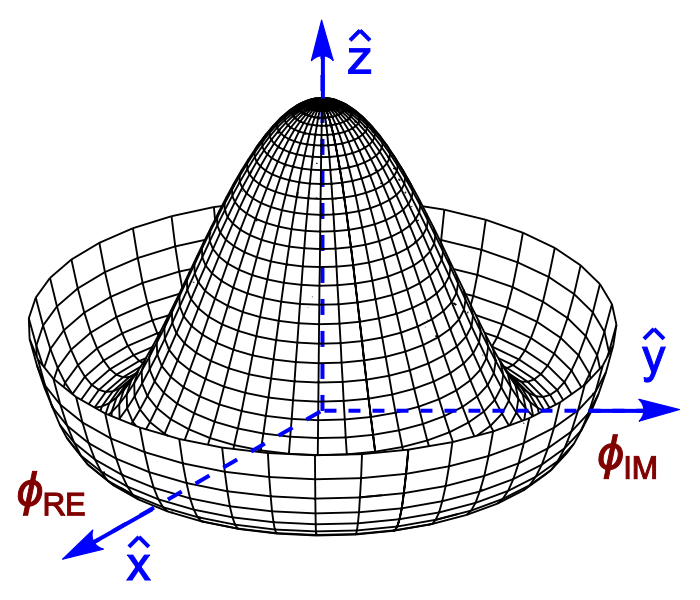
\includegraphics[width=0.6\textwidth]{figs/Mexican_hat.png}
    \caption{Complex scalar doublet potential.}
    \label{fig:MexicanHat}
  \end{center}
\end{figure}

\subsection{Brout-Englert-Higgs mechanism}
\label{sec:higgs}

After the spontaneous symmetry breaking, the scalar doublet transforms into the form given in equation~\ref{eq:TransHiggsDoublet}, where $G^{+}$ and $G^{0}$ are the Goldstone bosons from the breaking of the $SU(2)$ symmetry, and \Hb~is the Brout-Englert-Higgs boson. From Goldstone's theorem when a symmetry is spontaneously broken, a massless boson appears for each broken generator. In our specific case, the three generators of $SU(2)$ are broken giving rise to three Goldstone bosons: $G^{+}$, $G^{-}$ and $G^{0}$. This massless bosons are ``eaten'' by the $W^{+}$, $W^{-}$ and \Z~giving them an additional degree of freedom, the longitudinal polarization. 

\begin{equation}
  \label{eq:TransHiggsDoublet}
  \Phi=\left(
    \begin{array}{c}
      G^{+} \\
      \frac{1}{\sqrt(2)}(H+v-iG^{0})
    \end{array}
  \right)
\end{equation}

By this mechanism, the \W~and \Z~bosons acquire mass, being its value set by the coupling constant of $SU(2)$ group and the vacuum expectation value of Brout-Englert-Higgs boson. In addition, the fermions in the theory also acquire a mass from the interactions with the scalar doublet. Such masses are in general of the form $m_{f}=\lambda_{f}v/\sqrt(2)$, where $\lambda_{f}$ sets the interaction between the Brout-Englert-Higgs boson and the fermion. Finally, also the Brout-Englert-Higgs boson has a mass $m_{H}^{2}=-2\mu^{2}$.

In summary, with this mechanism the weak interaction bosons and fermions of the theory are given a mass at the price of introducing at least one additional scalar field to spontaneously break the $SU(2)$ symmetry.

\section{Hierarchy problem and other SM limitations}
\label{sec:hier}

The SM is certainly one of the most successful theories in the history of physics. With only 19 free parameters, it is able to make thousands of predictions that have been measured and tested over the last seventy to eighty years. However some aspects in the model are not completely understood. The most important one is the so-called hierarchy mass problem. At tree level, the Brout-Englert-Higgs boson has a mass $m_{H}^{2}=-2\mu^{2}$, but the physical mass also contains the one-loop contributions from particles that interact with it, as the top quark. The Feynman diagram for such contribution can be seen in figure~\ref{fig:oneloophiggs}.

\begin{figure}[!Hhtbp]
  \begin{center}
    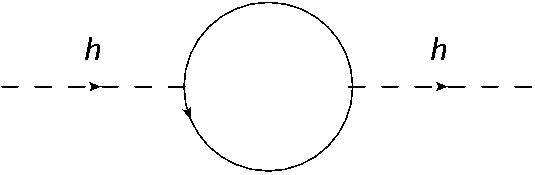
\includegraphics[width=0.6\textwidth]{figs/HierarchyLoop.png}
    \caption{One loop diagram for contributions to the mass of the Brout-Englert-Higgs boson from interactions with fermions}
    \label{fig:oneloophiggs}
  \end{center}
\end{figure}

Such contributions add up giving a mass greater than simple tree level mass. Each fermion contributes proportionally to its mass, which means that the top quark contributes the most. Moreover, if there are in nature heavier fermions that also interact with the Brout-Englert-Higgs boson they will also contribute to its mass. With such considerations the Brout-Englert-Higgs boson mass is expected to be much greater than 125 GeV, and in principle not even of the order of 100 GeV but greater than 1 TeV. However the real relevance or significance of this problem at theoretical level has been discussed extensively, for example at~\cite{Jegerlehner:2013nna}, the majority of the community agrees there is something to be understood on the subject. 

The most famous proposed solution to this problem is supersymmetry (SUSY)~\cite{Martin:1997ns}. It proposes the existence of an additional symmetry between fermions and bosons, at a given point of the history of universe nature did not distinguish between fermions and bosons. However, as it is known, this does not happen presently, that means this symmetry must be broken. Such symmetry implies the existence of a super-symmetric partner for each particle, a super-partner. A fermion for each boson and vice versa. This SUSY procedure doubles the particle content of the model where it is applied. Before breaking SUSY, a particle and its partner have the same mass. This characteristic solves the hierarchy problem in SUSY. Figure~\ref{fig:susy} shows the one loop diagrams for the mass of the Brout-Englert-Higgs boson from the top and its super-partner the stop. Whereas, the top contribution is positive, the stop contribution is negative but equal in value, then cancelling each other.

\begin{figure}[!Hhtbp]
  \begin{center}
    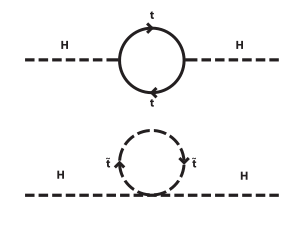
\includegraphics[width=0.6\textwidth]{figs/SUSY.png}
    \caption{One loop diagrams for contributions to the mass of the Brout-Englert-Higgs boson from the top and the stop}
    \label{fig:susy}
  \end{center}
\end{figure}

But this solution works exactly only if SUSY is not broken. As SUSY has to be broken, different ways have been proposed to break SUSY and still offer a solution to the hierarchy problem, leading essentially to solutions that need a fine adjustment of the parameters of the theory. This represents for some theoreticians a problem itself: fine-tuning or naturalness. Extensive searches for SUSY particles have been performed, accordingly to different models: MSSM~\cite{Khachatryan:2014wca,Aad:2014vgg}, CMSSM~\cite{Agashe:2014kda}, etc.

While hierarchy problem is an internal problem of the SM, there are however several questions that have not been solved. For example, how gravity is understood in the frame of QFT's? Why there is only 3 generations of leptons and quarks? Why there are 4 fundamental forces? In addition, there have been experimental questionings to the SM. The most important one is the masses of neutrinos. In the SM neutrinos are massless, careful measurements,~\cite{Ashie:2004mr, Weinheimer:2013hya}, have shown that neutrinos can oscillate between different flavors, phenomenon only possible if neutrinos have a mass. Measurements of solar and atmospheric neutrino oscillations have been the most important proofs of physics beyond the SM. 

From cosmological measurements, the Wilkinson Microwave Anisotropy Probe (WMAP) has shown that the universe is not only made by visible matter, but suggests that around 24\% it is made of dark matter, a type of matter not visible by means of light. It has also shown that 71\% of the universe is composed of dark energy, which makes the universe to be in an accelerated state of expansion. These results are shown in~\cite{2013ApJS..208...20B, 2013ApJS..208...19H}. Also the Planck probe has shown similar results, for example in~\cite{Planck:2015xua}. The SM does not have any answer to these open problems so far. 

Finally, it is known that the universe presents an asymmetry between matter and antimatter, the first being much more abundant than the second. Such asymmetry can be obtained by CP-violating processes (C for charge and P for parity). However the amount of CP violation in the SM is not compatible with the huge matter-antimatter asymmetry in nature. This problem, known as baryon asymmetry, represents an additional huge challenge for particle physics. 

In conclusion, the SM has been a formidable model that has helped the understanding of a huge amount of physics. It has done thousands of predictions that have been verified experimentally in the last half-century. However, this is not the end of the story, perhaps only the beginning. There are theoretical and experimental motivations that support the idea that the SM is not the ``final'' theory that could explain all subatomic phenomena in nature. Currently, there are a lot of efforts, both theoretical and experimental, to understand and explain all the remaining pieces. The present work is one of them.

In the next section, an extension of the SM that looks for a solution to the discussed hierarchy problem is presented. Chapter~\ref{chap:pheno} shows a strategy to look at LHC data for some of the predictions given by this SM extension.  %Then, principal productions predicted by the SM at the LHC involving particles, the top and the Higgs, used for new physics searches will be described. 

\section{Vector Like Quarks}

\label{chap:VLQ}

From last sections it has been shown how there are some parts in the SM that need further understanding. From such internal issues some further models/theories have been developed. All this theories are commonly grouped under the term Beyond Standard Model or simply BSM. One of the most famous BSM theory is supersymmetry (SUSY). This idea have given birth to a plethora of model realizations and physics predictions. So far, none of the new consequences of this theory have been confirmed but the experiments have an enormous investment on their search. But not only SUSY have seen the day light, there is on the market an astonishing amount of BSM theories addressing different issues of the SM. Extra dimensions, fourth families, composite Higgs are a few of them.

In this section a bunch of models that introduce additional heavy quarks, heavier than the top, in order to solve the hierarchy problem will be described. %, described in section~\ref{sec:hier}. 

\subsection{Theoretical motivation}
\label{sec:motiv}

Even tho the SM has 3 families, the number of families in nature is not restricted by any fundamental principle. However, searches for fourth families have not found any evidence of additional families in nature~\cite{Eberhardt:2012gv}. But a fourth family formulation relies on the existence of a sequential additional family, this is for the quark sector, two additional quarks, heavier than the top with the same quantum number structure as the other 3 families. In particular the 3 SM families are formed by doublets of the left components of quark fields. 

Fermionic fields can be divided in terms of two chiral components. The chirality is related to the relative orientation of the momentum and spin of a particle. A particle is said to have right chirality if its momentum and spin are aligned and left chirality if they are anti-aligned.  Accordingly to electroweak theory the only left fermions undergo weak interactions, reason why SM quark families are left. 

Nothing prevents to formulate a model where new quarks right and left components are subjected to weak interaction indistinctly. A fermion having identical left and right chiralities is called vector-like. These type of models introduce only new quarks without need of a full new family.

This new top-like states allow to have a suitable solution for the hierarchy problem. They arise typically in Kaluza-Klein extra dimension models~\cite{Contino:2006qr, Matsedonskyi:2012ym, Dissertori:2010ug}. In more generic modeling of vector-like quarks (VLQ) these new states are added to the SM content as an electroweak representation (singlet or doublet) coupled to SM quarks.

\subsection{Generic Formulation}
\label{sec:form}

The generic formulation that is going to be described is based on~\cite{Buchkremer:2013bha, Cacciapaglia:2011fx}.

In a very generic conception, vector-like quarks can be added to the SM content as being part of an electroweak representation. Introduced with the same color charge than SM quarks they can come in 4 different forms depending of their electric charge:
\begin{itemize}
\item $X$ with 5/3 electric charge
\item \Tp~with 2/3 electric charge, as the top quark.
\item $B$ with -1/3 electric charge, as the bottom quark.
\item $Y$ with -4/3 electric charge.
\end{itemize}

The \Tp~is also called in the literature a top partner. Given VLQ electric charges they can be arranged in different representations. Table~\ref{tab:VLQRepre} displays the plausible different electroweak representations of VLQ. The $\binom{X}{T}$ and $\binom{T}{B}$ doublet will referred as the non-standard and standard doublet respectively.  

\begin{table}[htbH]
\begin{center}
\begin{tabular}{|c|c|c|c|c|c|c|}
\hline 
 & SM & \multicolumn{2}{c|}{Singlets} & \multicolumn{3}{c|}{Doublets} \\
 & $\binom{u}{d}$ $\binom{c}{s}$ $\binom{b}{t}$ & \Tp & B & $\binom{X}{T'}$ & $\binom{T'}{B}$ & $\binom{B}{Y}$ \\ 
\hline
$SU(2)_{L}$ & 2 & \multicolumn{2}{c|}{1} & \multicolumn{3}{c|}{2} \\ \hline
$U(1)_{Y}$ & $q_{L}=1/6$; $u_{R}=2/3$; $d_{R}=-1/3$ & 2/3 & -1/3 & 1/6 & 7/6 & -5/6 \\
\hline
\end{tabular}
\caption{Possible VLQ representations and corresponding $SU(2)_{L}\times U(1)$ charges and SM quarks. \label{tab:VLQRepre}}
\end{center}
\end{table}

The effective Lagrangian for a general formulation of VLQ, restricting it for \Tp~and $X$ type of vector-like quarks in the non-standard doublet is the following:
\begin{eqnarray}
  \mathcal{L} & = & \kappa_{T}\left\{ \sqrt{\frac{\zeta_{i}\xi_{Z}^{T}}{\Gamma_{Z}^{0}}}\frac{g}{2c_{W}}\left[ \bar{T'}_{R}Z_{\mu}\gamma^{\mu}u^{i}_{R}\right]\right\} 
               -  \kappa_{T}\left\{ \sqrt{\frac{\zeta_{i}\xi_{H}^{T}}{\Gamma_{H}^{0}}}\frac{M}{v}\left[ \bar{T'}_{L}Hu^{i}_{R}\right] + \sqrt{\frac{\zeta_{3}\xi_{H}^{T}}{\Gamma_{H}^{0}}}\frac{m_{t}}{v}\left[ \bar{T'}_{R}Ht_{L}\right]\right\} \nonumber\\            
              & + & \kappa_{X}\left\{ \sqrt{\frac{\zeta_{i}}{\Gamma_{W}^{0}}}\frac{g}{\sqrt{2}}\left[ \bar{X}_{R}W^{+}_{\mu}\gamma^{\mu}u^{i}_{R}\right]\right\} +h.c.
\label{eq:VLQLag}
\end{eqnarray} 
neglecting terms proportional to the light quark masses. In addition, terms proportional to top mass can also be neglected as they only introduce differences of only 10\%-20\% for \Tp~masses below 600 GeV. The parameters $\kappa_T$, $\kappa_X$ are the coupling strengths and determine the strength of the VLQ production. In equation~\ref{eq:VLQLag}, $M$ represents the \Tp~mass, $m_{t}$ the top mass, $\zeta_{i}$ the coupling between VLQ and the $i$th SM quarks generation, $\xi_{Z}^{T}$ and $\xi_{H}^{T}$  the mixing of \Tp~with the $Z$ and Higgs boson respectively. Finally, $v$ and $g$ are the usual vacuum expectation value and electroweak coupling in the SM, and $\Gamma^{0}_{i}$ the width of the boson $i=W^{+/-},Z^{0},H^{0}$.
%\begin{TOINCLUDE}Table with different possible representations and assigned charges\end{TOINCLUDE}

\subsubsection{Production modes}
\label{sec:prod}

VLQ can be produced singly or pairwise, as the SM top quark. Pair production is dominated by QCD processes via gluons, as shown in figure~\ref{fig:ProdDiagPair}. Additional contributions are given via the a t-channel exchange of a vector boson. For example, figure~\ref{fig:ProdDiagPair} shows the production process via the \Z~boson that produce two same sign VLQ.   

Single production is mainly mediated by a vector boson via a t-channel in association with a SM quark. In figure~\ref{fig:ProdDiagSingle} the Feynman diagram for \Tp~single production with a SM quark is shown. In addition, the \Tp~can be also produced with a \Z~or \W~boson or a Higgs from an initial gluon-quark fusion. 

The VLQ production cross section in proton-proton collision strongly depends from their mixings to SM quarks. Historically, top partners have been modeled with exclusive mixings to third generation SM quarks. In the generic formulation being considered, the VLQ can mix to the three SM quark generations. In particular the case where couplings to light generations are important has been considered for the present work. Figure~\ref{fig:TProdXS}, from~\cite{Cacciapaglia:2011fx}, shows the \Tp~production cross sections in pairs and singly in proton-proton collisions. For $T$ masses higher than 400 GeV the single production is dominant with regard to pair production. 

\begin{figure}[!Hhtbp]
  \begin{center}
    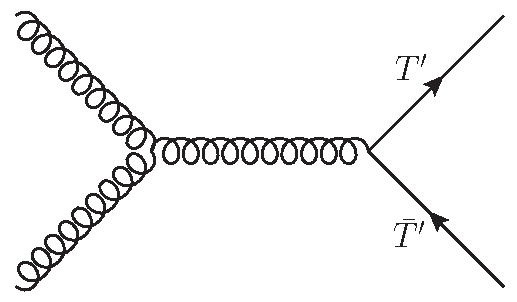
\includegraphics[width=0.3\textwidth]{figs/Gluon_fusion_T_pair.jpg}
    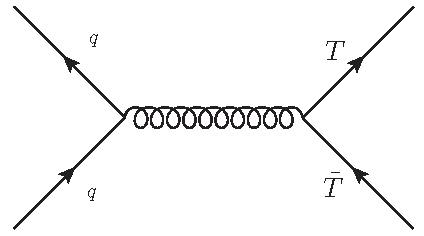
\includegraphics[width=0.3\textwidth]{figs/Quarks_schannel_T_pair.jpg}
    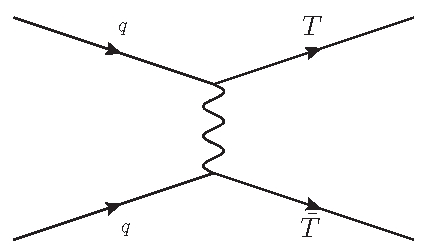
\includegraphics[width=0.3\textwidth]{figs/Gluon_tchannel_T_pair.jpg}
    \caption{Feynman diagrams of \Tp~production in pairs}
    \label{fig:ProdDiagPair}
  \end{center}
\end{figure}

\begin{figure}[!Hhtbp]
  \begin{center}
    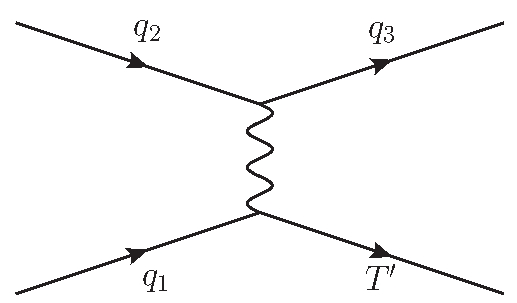
\includegraphics[width=0.45\textwidth]{figs/Tchannel_T_single.jpg}
    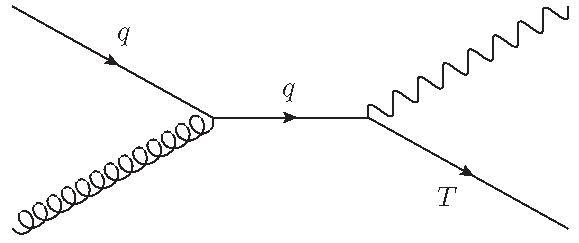
\includegraphics[width=0.45\textwidth]{figs/QuarkGluonFusion_SingleT.jpg}
    \caption{Single \Tp~production Feynman diagrams}
    \label{fig:ProdDiagSingle}
  \end{center}
\end{figure}

\begin{figure}[!Hhtbp]
  \begin{center}
    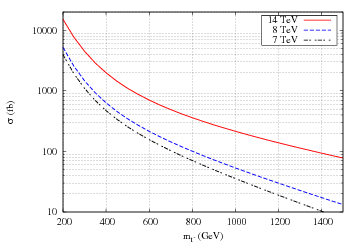
\includegraphics[width=0.45\textwidth]{figs/pheno_prod_single_tp.png}
    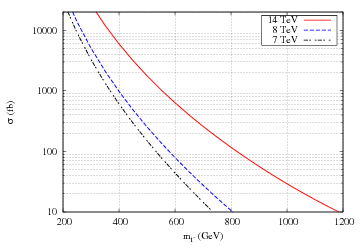
\includegraphics[width=0.45\textwidth]{figs/pheno_prod_pair_tp.png}
    \caption{$T$ production cross section for single [left] and pair [right] channels as function of \Tp~mass for different center of mass energy in proton-proton collisions.}
    \label{fig:TProdXS}
  \end{center}
\end{figure}
%\begin{TOINCLUDE}Plot of production cross section at LHC for different energies as function of the mass. Feynman diagrams of the production processes.\end{TOINCLUDE}

\subsubsection{Decay modes}
\label{sec:decay}

The parameters $\zeta_{i}$ and $\xi_i$, from the Lagrangian in equation~\ref{eq:VLQLag}, are directly linked to the branching ratios:
 \begin{eqnarray} 
BR (T' \to Z^{0} j) = \frac{\zeta_{jet} \xi^T_Z}{1+\zeta_3 \xi_H \delta_H}\,, & & BR (T' \to Z^{0} t) = \frac{(1-\zeta_{jet}) \xi^T_Z}{1+\zeta_3 
\xi_H \delta_H}\,,\\
BR(T' \to H^{0} j) = \frac{\zeta_{jet} (1-\xi^T_Z)}{1+\zeta_3 \xi_H \delta_H}\,, & &  BR(T' \to H^{0} t) = \frac{(1-\zeta_{jet})
(1-\xi^T_Z) (1+\delta_H)}{1+\zeta_3 \xi_H \delta_H}\,, \nonumber\\
 & & \nonumber \\
BR(X \to W^{+} j) = \zeta_{jet}\,, & & BR(X \to W^{+} t) = (1-\zeta_{jet})
 \end{eqnarray} where $\zeta_{jet}$ accounts for the contributions of the two light quark generations and $j$ for jet.

The branching fractions of the top partner \Tp~only depend on the two parameters $\zeta_{jet}$ and $\xi_Z^{T}$, as $\delta_H$ is a calculable function of the heavy mass scale for the vector-like quarks $M$:
\begin{eqnarray} 
\delta_H  \sim 5 \frac{m^2_t}{M^2}\,, \label{eq:deltaH}
\end{eqnarray} 
where only the leading order in $1/M^2$ has been kept. Note that in these formulae the decay rates into \Z~and \Hb~are kept arbitrary (parameterised by $\xi_Z^{T}$ which is equal to 1/2 for the non-standard doublet case). These approximate but quite robust results allow to describe easily the phenomenology of the non-standard doublet. 

For a \Tp~coming from other representations the situation is not much different in terms of decay modes, as only the extra decay to $W$ and quarks will be present. In figure~\ref{fig:TBRs} are presented the branching ratios of \Tp~as function of its mass, taken from~\cite{Cacciapaglia:2011fx}. It is important to notice that for masses higher than 300 GeV the decay channel into top-Higgs become dominant.

\begin{figure}[!Hhtbp]
  \begin{center}
    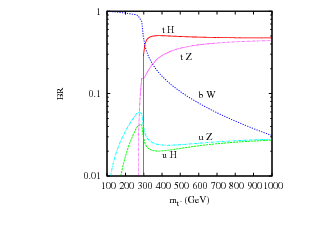
\includegraphics[width=0.8\textwidth]{figs/pheno_br_tp.png}
    \caption{\Tp~branching ratios as function of its mass.}
    \label{fig:TBRs}
  \end{center}
\end{figure}

In the present work, a search for a \Tp~will be described. This search looked for the \Tp~when it decays into a top quark and a Higgs boson. Therefore is important to understand the properties of this particles and how they are produced in the LHC, as predicted by the SM. In the next sections the production of these SM particles at the LHC and their specific properties are going to be presented. %In particular the top and the Higgs, constantly used for new physics searches will be described.

\section{Top at the LHC}
\subsection{Top production}

Discovered in 1995 by D\O~\cite{Abazov:2002su} and CDF~\cite{Blair:1996kx} collaborations at Tevatron~\cite{Group:1984bk,Holmes:2011nq}, it is the heaviest fundamental particle known. As heaviest particle, many models beyond the SM predict a coupling of the top quarks with a heavier new physics sector. It forms a $SU(2)_{L}$ weak isospin doublet with the b-quark, discovered in 1977. Their mass difference, two orders of magnitude, is a fundamental question in the SM. Precision measurements of the top quark characteristics are fundamental inputs to test the SM and new physics searches.

The LHC can be seen as a top-factory, being the accelerator where the most of top-quarks can be produced. The top quark is produced in pairs and singly. During run 1, taking into account 7 TeV and 8 TeV data, 5.6 millions of top pairs events and 2.7 millions of single top events were delivered by the LHC to ATLAS and CMS experiments. Taking into account the different cross sections of the production processes, that will be discussed in the following sections, and the instantaneous luminosity, cited in table~\ref{tab:LHCparams}, for 8 TeV center of mass energy, at LHC around 6 tops per second are produced, where 5 of them come from top-pair events and one from single-top events.  

\subsubsection{Pair production}
\label{subsec:toppair}

Top pair production constitutes the dominant production channel in proton-proton collisions at LHC. Its high cross section makes this process one of the most important background for searches of new physics at LHC. Latest theoretical calculations at Next-to-Next-to-Leading-Order (NNLO)~\cite{Czakon:2013goa}, see section~\ref{sec:parton}, of top pair production from proton-proton collisions at $\sqrt{s}=8$ TeV give a cross section $\sigma_{t\bar{t}}=247.47$ pb with around 5\% total uncertainty. The tree level diagrams that contribute to this production are summarized in figure~\ref{fig:PairProductionFD}, where gluon fusion dominates the pair production. At $\sqrt{s}=13$ TeV, as for LHC Run 2, this cross section will scale about 3.3 times. Comparison between theoretical predictions and experimental measurements of top pair production is shown in figure~\ref{fig:PairProduction}, taken from~\cite{TOPLHCWG}.

\begin{figure}[!Hhtbp]
  \begin{center}
    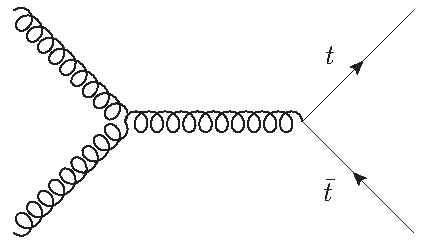
\includegraphics[width=0.32\textwidth]{figs/Gluon_fusion_top_pair.jpg}
    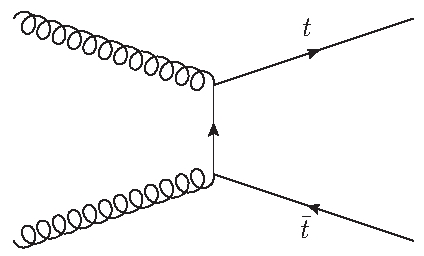
\includegraphics[width=0.32\textwidth]{figs/Gluon_tchannel_top_pair.jpg}
    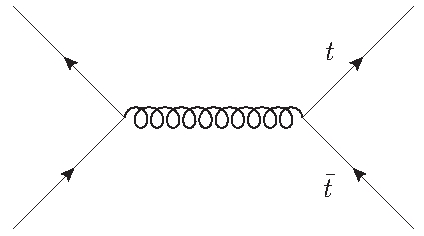
\includegraphics[width=0.32\textwidth]{figs/Quarks_schannel_top_pair.jpg}
    \caption{Top pair production processes Feynman diagrams for proton-proton collisions, via gluon fusion [left], gluon t-channel [middle] and quark-antiquark annihilation [right]}
    \label{fig:PairProductionFD}
  \end{center}
\end{figure}

\begin{figure}[!Hhtbp]
  \begin{center}
    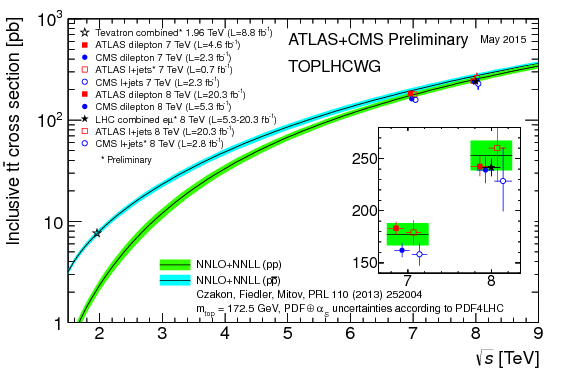
\includegraphics[width=0.9\textwidth]{figs/toplhcwg_ttxsec_sqrts_may2015.png}
    \caption{$t\bar{t}$ production cross section as function of the center of mass energy in $p\bar{p}$ and $pp$ collisions compared to theoretical predictions.}
    \label{fig:PairProduction}
  \end{center}
\end{figure}

%\begin{TOINCLUDE}Plots of cross section of ttbar production as function of center of mass energy; Feynman diagrams for pair production\end{TOINCLUDE}

\subsubsection{Single $t$ production}
\label{subsec:topsing}

A subdominant production process of top quark is the single production channel, where the top quark is produced in association with another quark, mediated by a $W$ boson, or with a $W$ boson. The Feynman diagrams for tree level single top production can be seen in figure~\ref{fig:SingleProductionFD}. NNLO predictions have been also done for these three single production modes, at $\sqrt{s}=8$ TeV. The cross sections are respectively: $\sigma_{t,\; \text{s-channel}}=5.56\pm4\%$ pb, $\sigma_{t,\; \text{t-channel}}=84.34\pm2\%$ pb and $\sigma_{tW}=22.2\pm3\%$ pb. Due to the high cross section of pair production compared to single production channels, the cross section measurement of each production mode has been difficult. The Tevatron was able to confirm the $s$ and $t$-channels~\cite{Aaltonen:2009jj}, while at LHC the $tW$ channel was confirmed~\cite{Chatrchyan:1642680}. The comparison of theoretical predicted cross section and experimental measurements, by ATLAS and CMS, at different center of mass energies is p[resented in figure~\ref{fig:SingleProduction}, taken from~\cite{TOPLHCWG}.

\begin{figure}[!Hhtbp]
  \begin{center}
    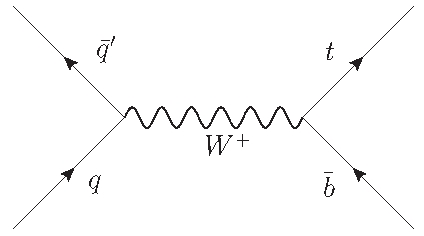
\includegraphics[width=0.32\textwidth]{figs/Schannel_top_single.jpg}
    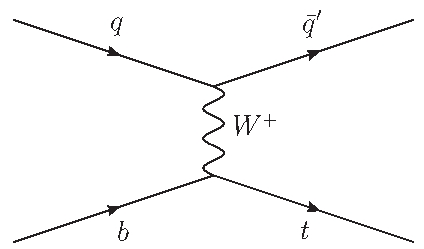
\includegraphics[width=0.32\textwidth]{figs/Tchannel_top_single.jpg}
    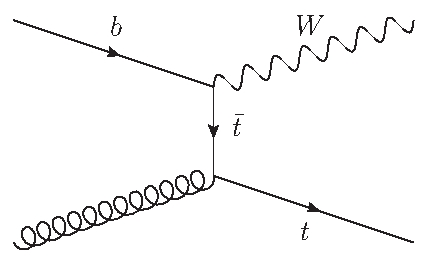
\includegraphics[width=0.32\textwidth]{figs/TWchannel_top_single.jpg}
    \caption{Single top production processes Feynman diagrams for proton-proton collisions, from left to right s-channel, t-channel and associated $W$ production.}
    \label{fig:SingleProductionFD}
  \end{center}
\end{figure}

\begin{figure}[!Hhtbp]
  \begin{center}
    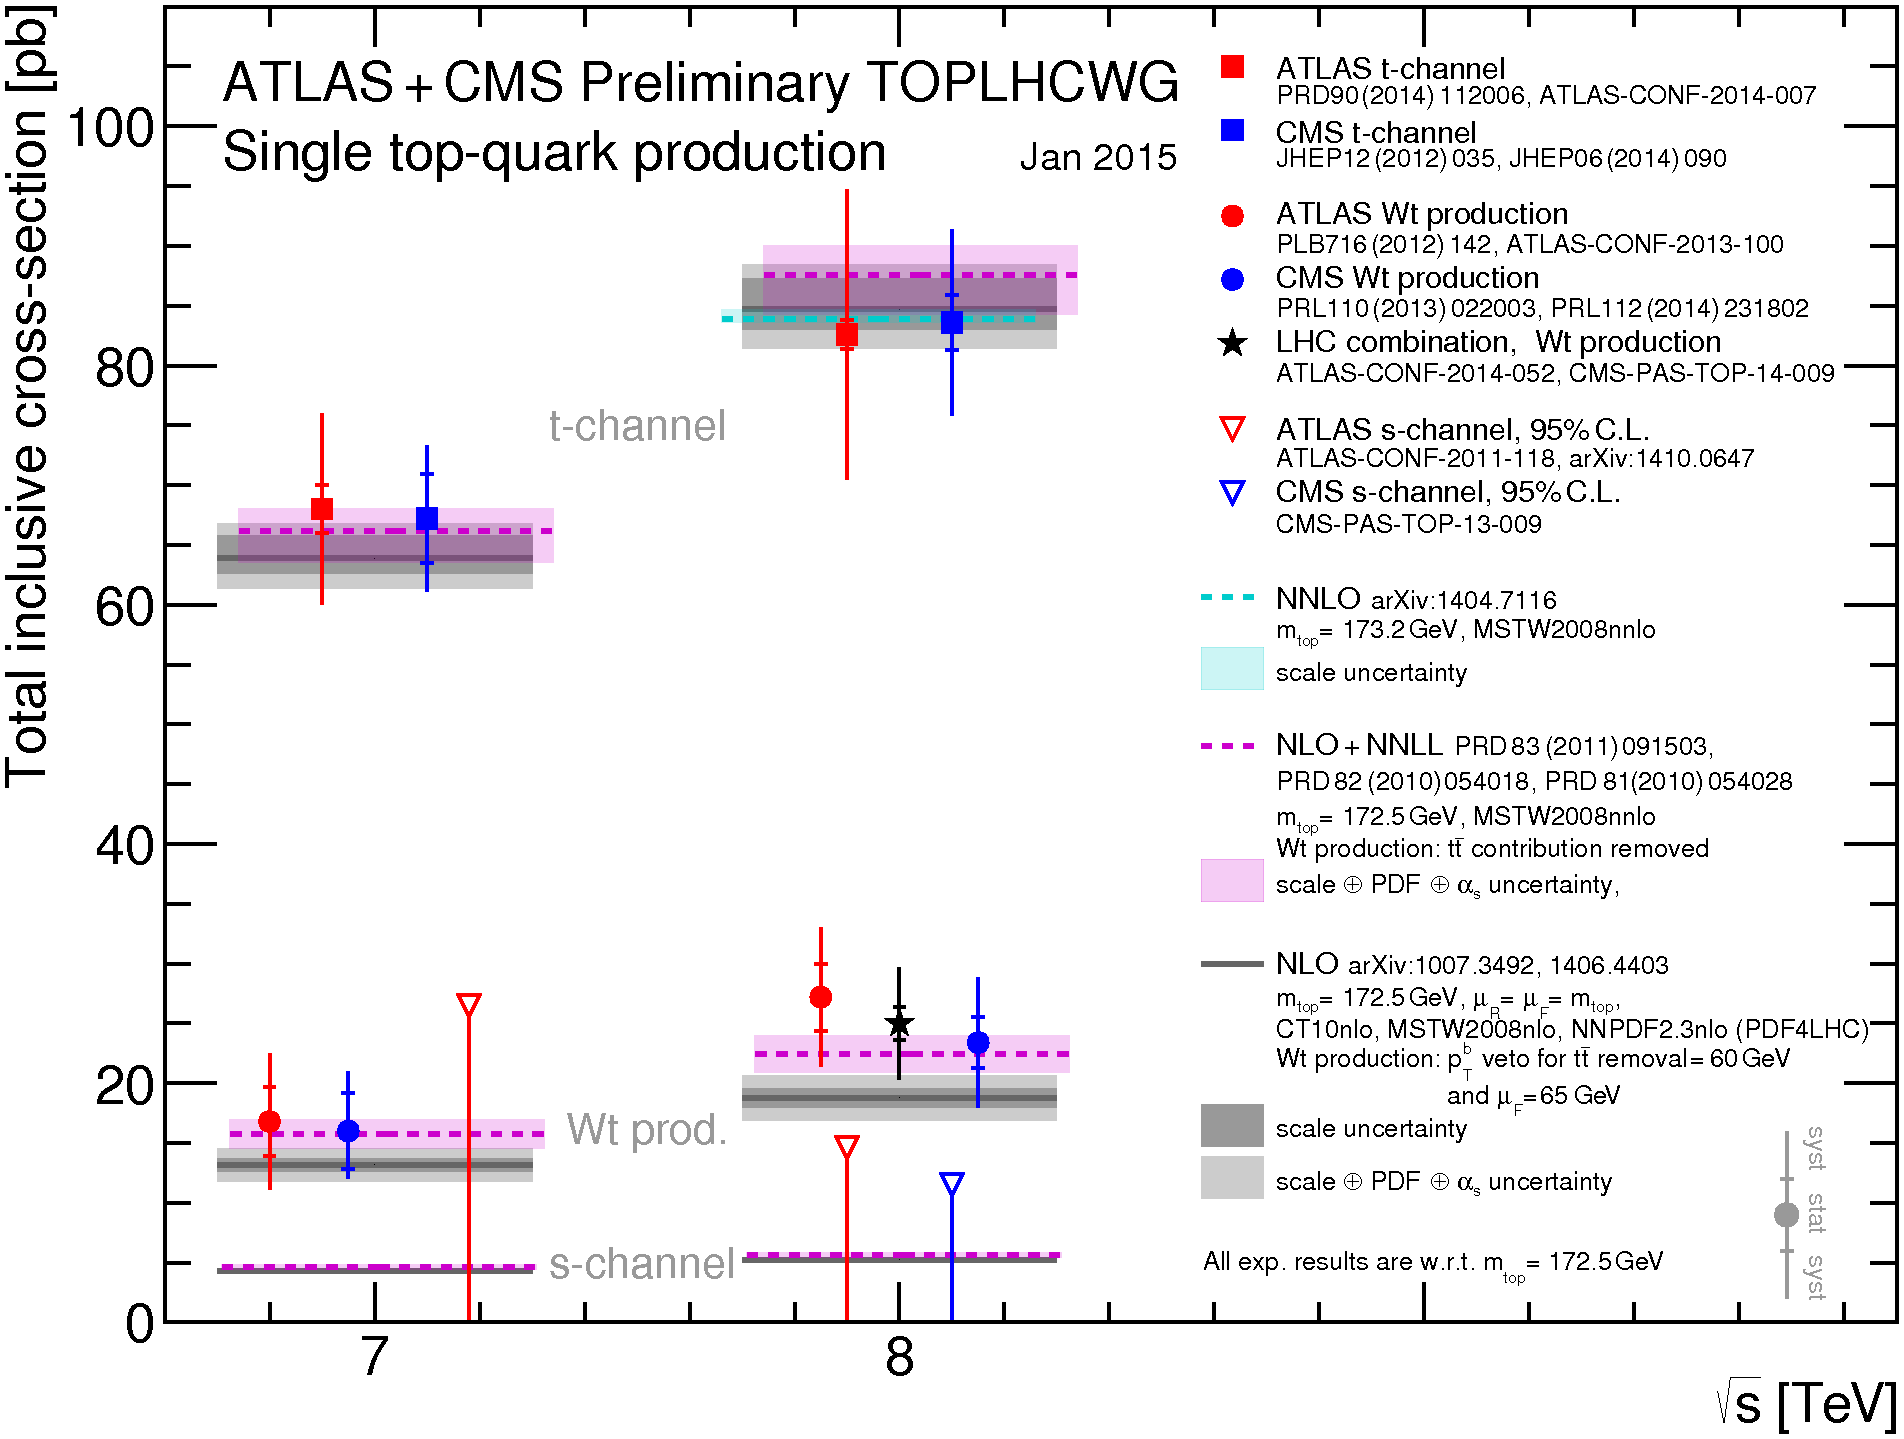
\includegraphics[width=0.9\textwidth]{figs/singletop_allchanvsroots.png}
    \caption{Single top production cross section as function of the center of mass energy in proton-proton collisions compared to theoretical predictions for each production channel by ATLAS and CMS collaborations.}
    \label{fig:SingleProduction}
  \end{center}
\end{figure}

%\begin{TOINCLUDE}Plots of cross section of single-top production as function of center of mass energy; Feynman diagrams for single production\end{TOINCLUDE}

\subsection{Top decay channels}

The top quark decays extremely fast, a process taking only $3\times 10^{-25}$ second. Hadronization processes occur around $3\times 10^{-24}$ which means that the top quark decays even before hadronization begins. Therefore it is the only quark that can be studied before hadronization, in its free state. According to CKM (Cabibbo–Kobayashi–Maskawa) matrix, that describes how different quarks interact between them, the top quark decays preferentially to a b-quark and a $W$ boson, 99\% of the times~\cite{Agashe:2014kda}. 

Then \W boson can decay into a lepton and a neutrino, or into a pair of quarks. The branching ratio of leptonic decays of \W boson is around 33\% while to quarks is 67\%~\cite{Agashe:2014kda}, being then the hadronic final state dominant. In figure~\ref{fig:BRratiosandDecayChannels} can be seen the two decay modes of top quark with their respective branching ratio. 

\begin{figure}[!Hhtbp]
  \begin{center}
    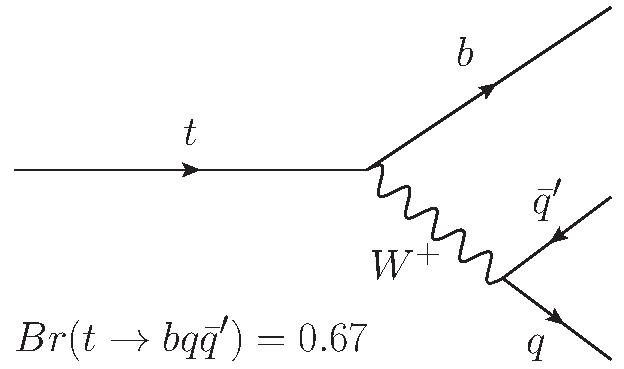
\includegraphics[width=0.4\textwidth]{figs/Top_H_Decay.png}
    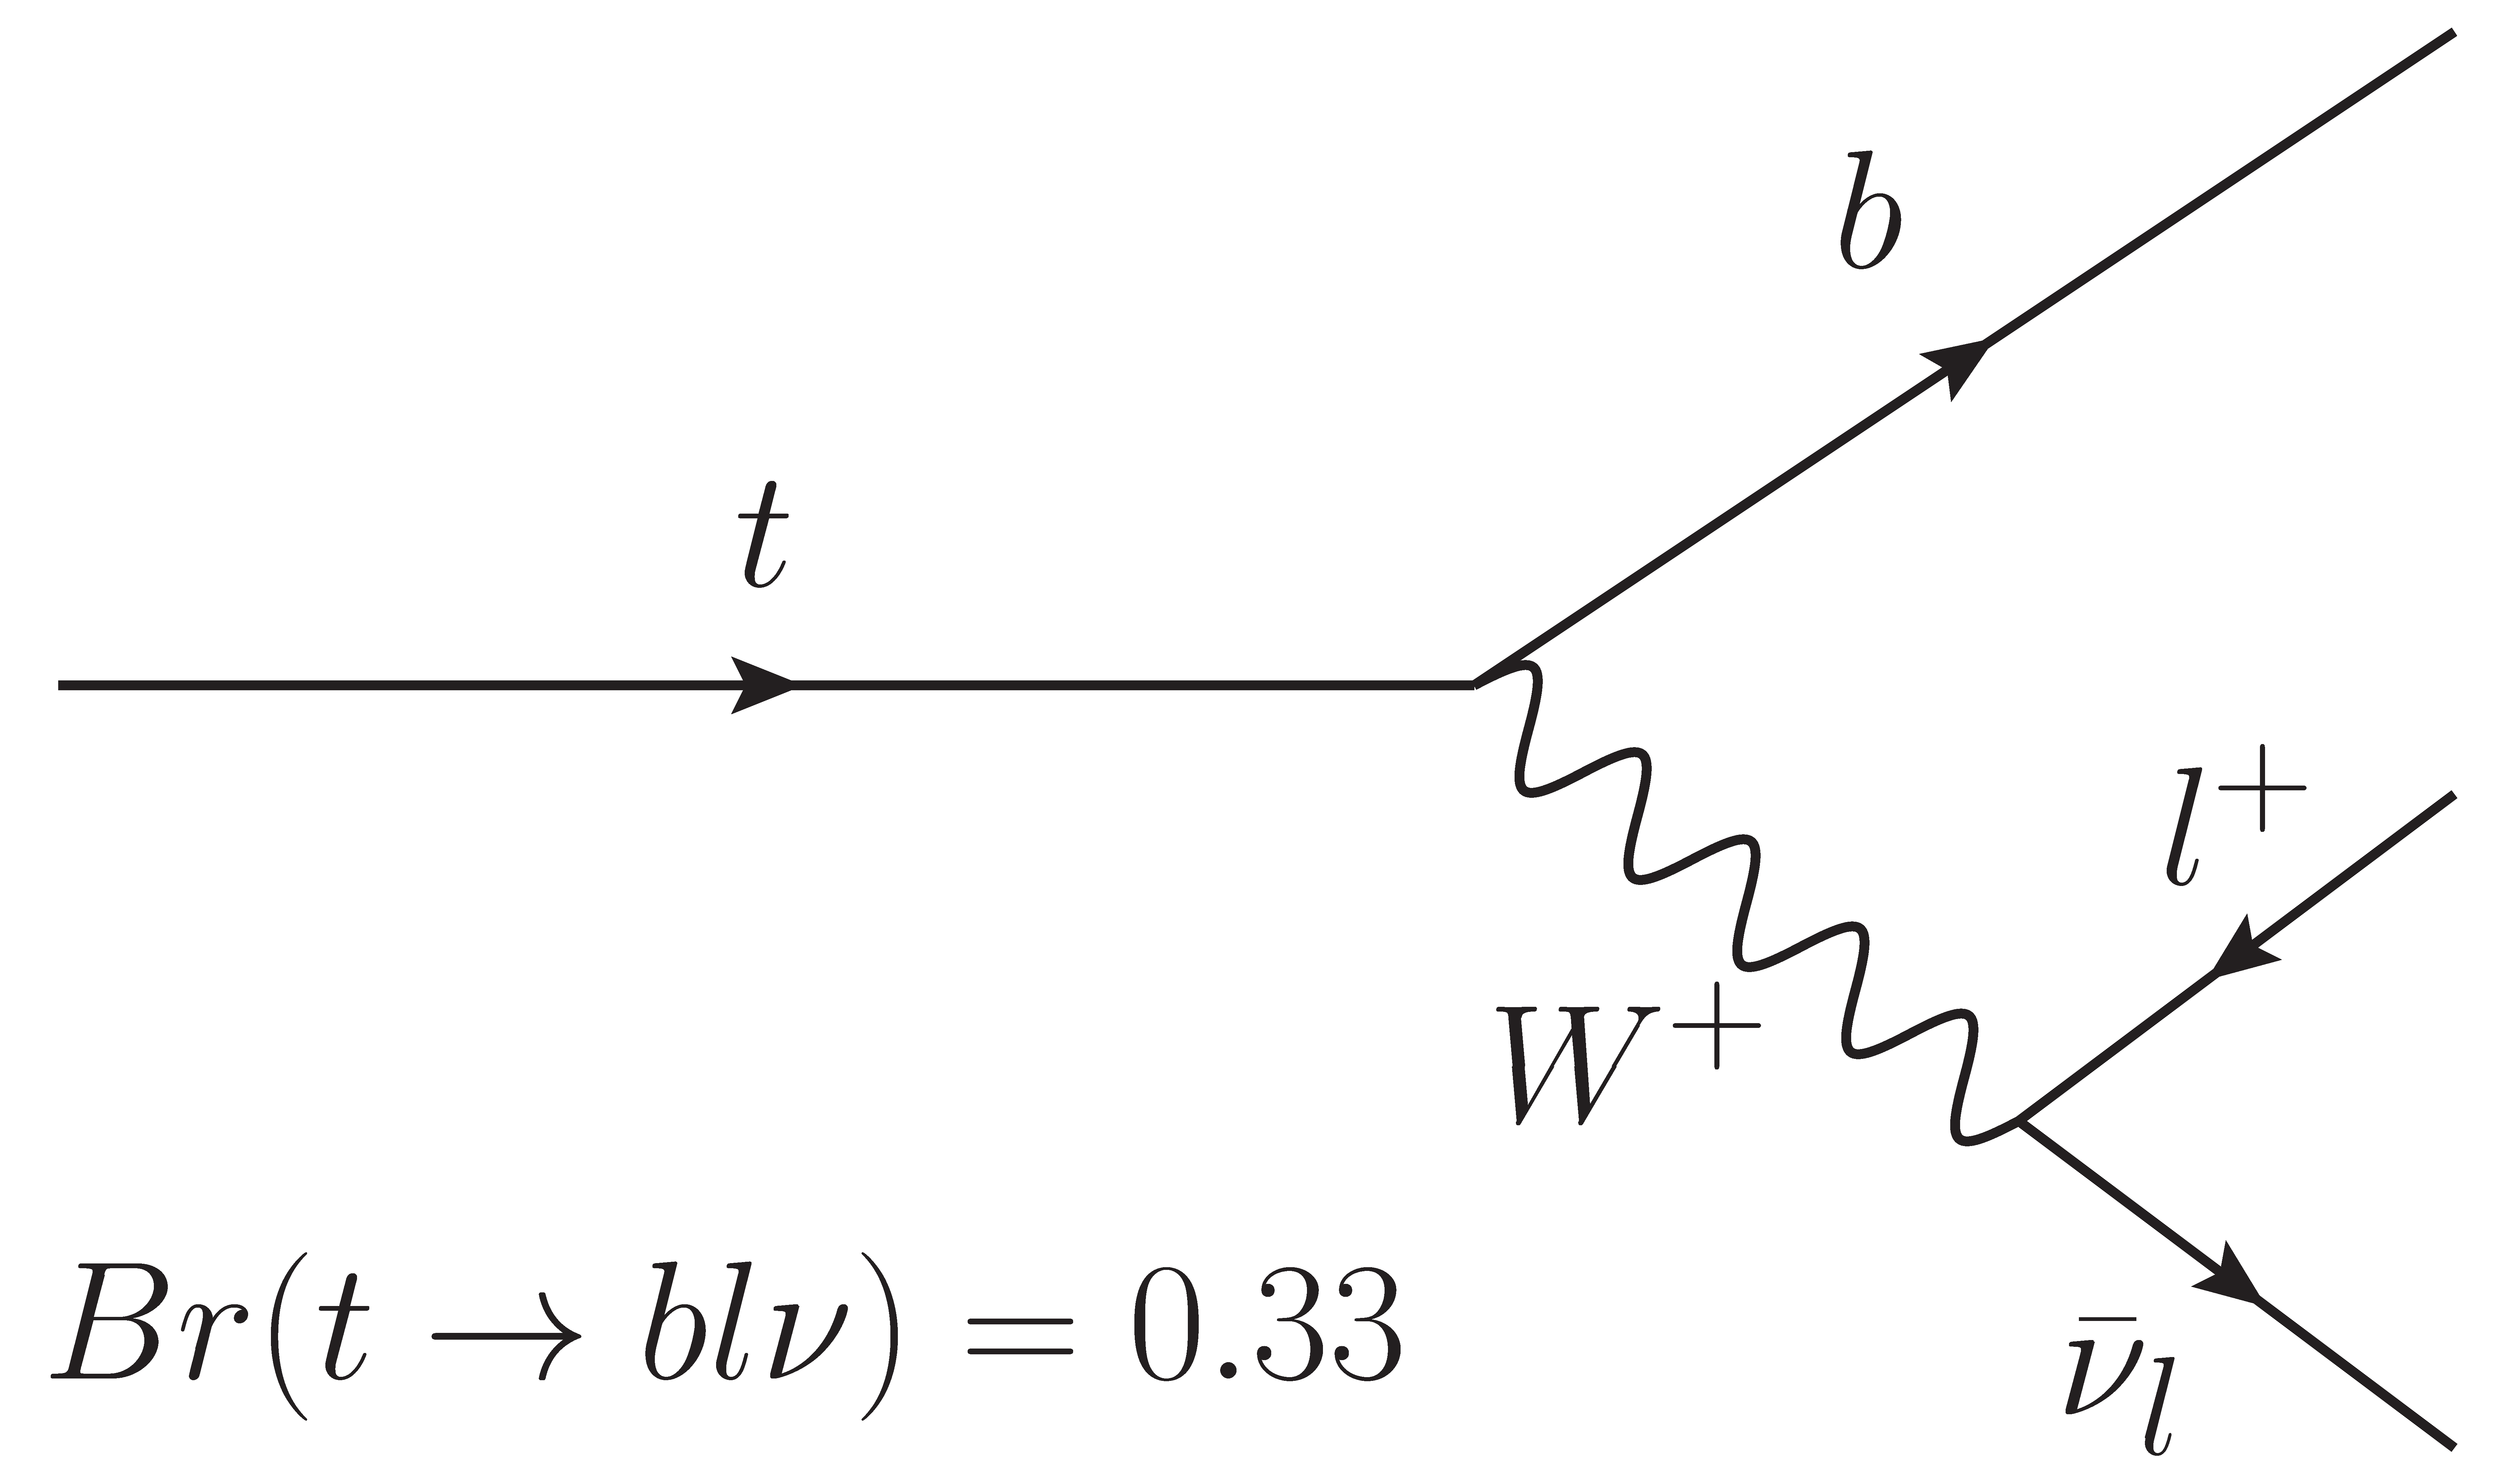
\includegraphics[width=0.4\textwidth]{figs/Top_L_Decay.png}
    \caption{Feynman diagrams for top decay channels with respective branching ratios.}
    \label{fig:BRratiosandDecayChannels}
  \end{center}
\end{figure}

%\begin{TOINCLUDE}Plot on possible decay channels and branching ratios to each channel; Feynman diagram for each decay channel\end{TOINCLUDE}
%
%\subsection{Top properties}
%
%Description of top properties and the measurement of them.
%
%\subsubsection{Electric charge}
%
%Top charge related to its decay.
%
%\subsubsection{Lifetime}
%
%Discussion on the importance of measurements of top as only quark decaying before hadronization time.

\subsection{Mass and width of top quark}

One of the most important quests in top physics is the measurement of top mass and width. They constitute two powerful tests of SM predictions. Whereas the top mass is a free parameter in the SM, actually it is constrained by other measurements, specially electroweak precision tests. Any deviation with respect to the expectation of the SM could point to the existence of new physics beyond the standard model. The width is also predicted by the SM.% and then it needs to be measured in experiment. 

At Next-to-Leading-Order (NLO)~\cite{Jezabek19891}, the SM expected value of top width is $\Gamma_{t}=1.27$ GeV. It depends of the top mass, the strong force coupling $\alpha_{S}$, the mass of the $W$ boson and the strength of the interaction between the top and b-quark. Present measurements have found $\Gamma_{t}=2.00^{+0.47}_{-0.43}$ GeV~\cite{Abazov:2012vd}, value in agreement with SM predictions. 

Top mass has been measured by ATLAS and CMS collaborations at LHC and by CDF and D\O~at Tevatron for each decay channel of top both in single and pair production. Current world combination is $m_{t}=173.34\pm 0.76$. Results from current searches and their combinations are presented in figure~\ref{fig:TopMass}, taken from~\cite{TOPLHCWG}. 

\begin{figure}[!Hhtbp]
  \begin{center}
    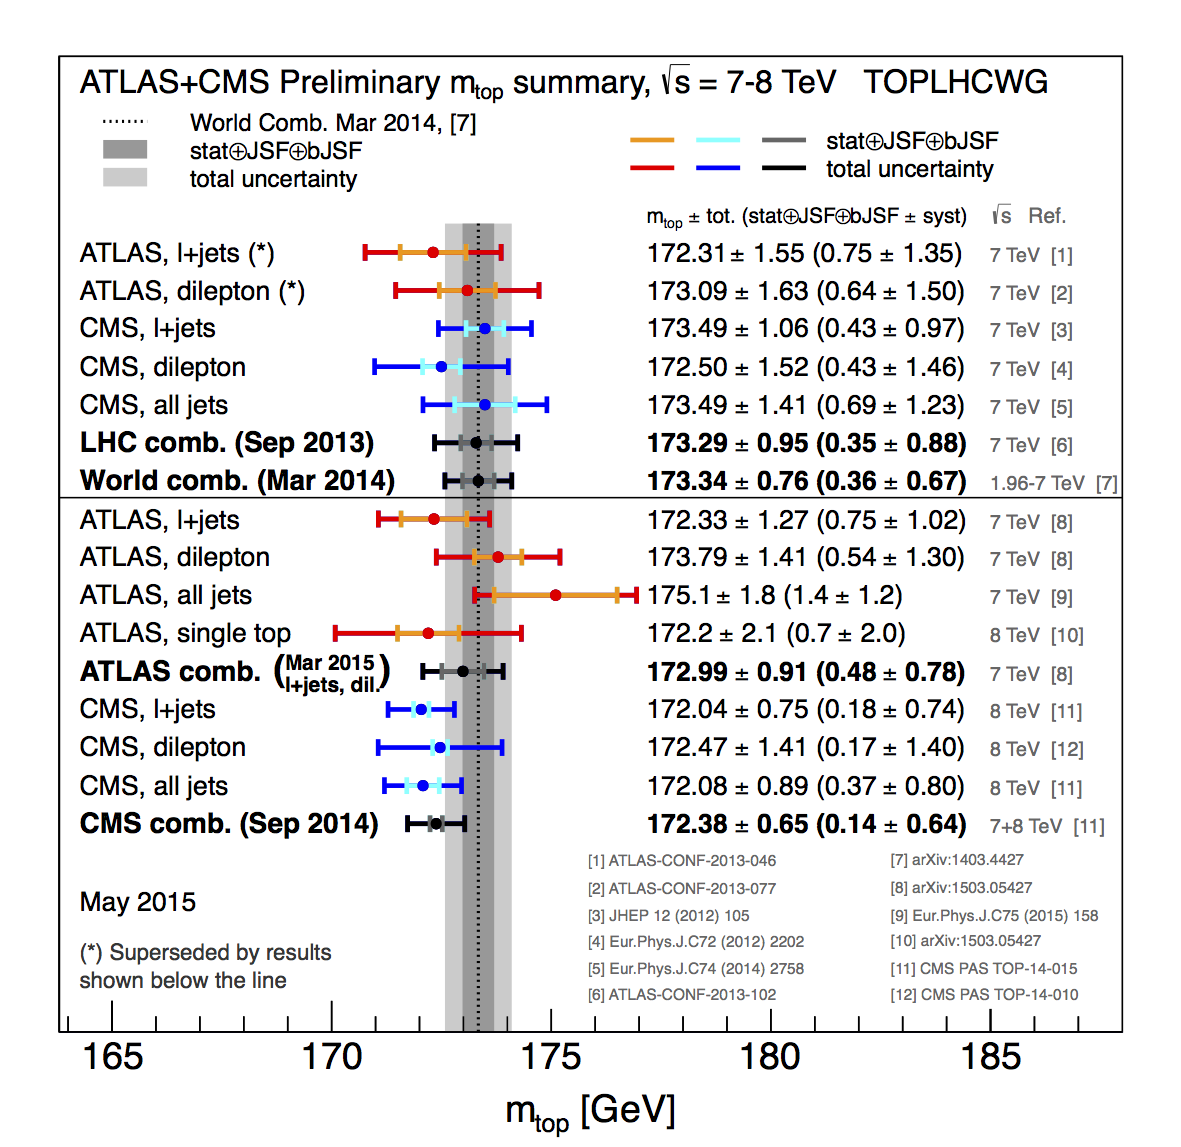
\includegraphics[width=0.9\textwidth]{figs/LHC_topmass_May2015.png}
    \caption{Top mass measurements from ATLAS and CMS collaborations and world combination including Tevatron results.}
    \label{fig:TopMass}
  \end{center}
\end{figure}

%\begin{TOINCLUDE}Plot of top mass measurement from Tevatron+LHC combination\end{TOINCLUDE}
%
%\subsubsection{Spin correlation}
%
%Discussion on how ttbar system have spin correlation that will be important for precision measurements.

\section{Higgs at the LHC}
\subsection{Higgs production}

The SM Higgs boson is expected to be produced in proton-proton collisions at LHC by four different processes: gluon fusion, via the fusion of two gluons via a top loop, Higgsstrahlung, where a Higgs boson is radiated from a $Z$ or $W$ boson, vector boson fusion, by the fusion of two vector bosons radiated from quarks, and quark fusion, from the fusion of quarks produced by a gluon splitting. Feynman diagrams for these processes can be seen in figure~\ref{fig:HiggsProd}. 

\begin{figure}[!Hhtbp]
  \begin{center}
    \includegraphics[width=0.42\textwidth, height=4cm]{figs/GluonFusion_H.png}
    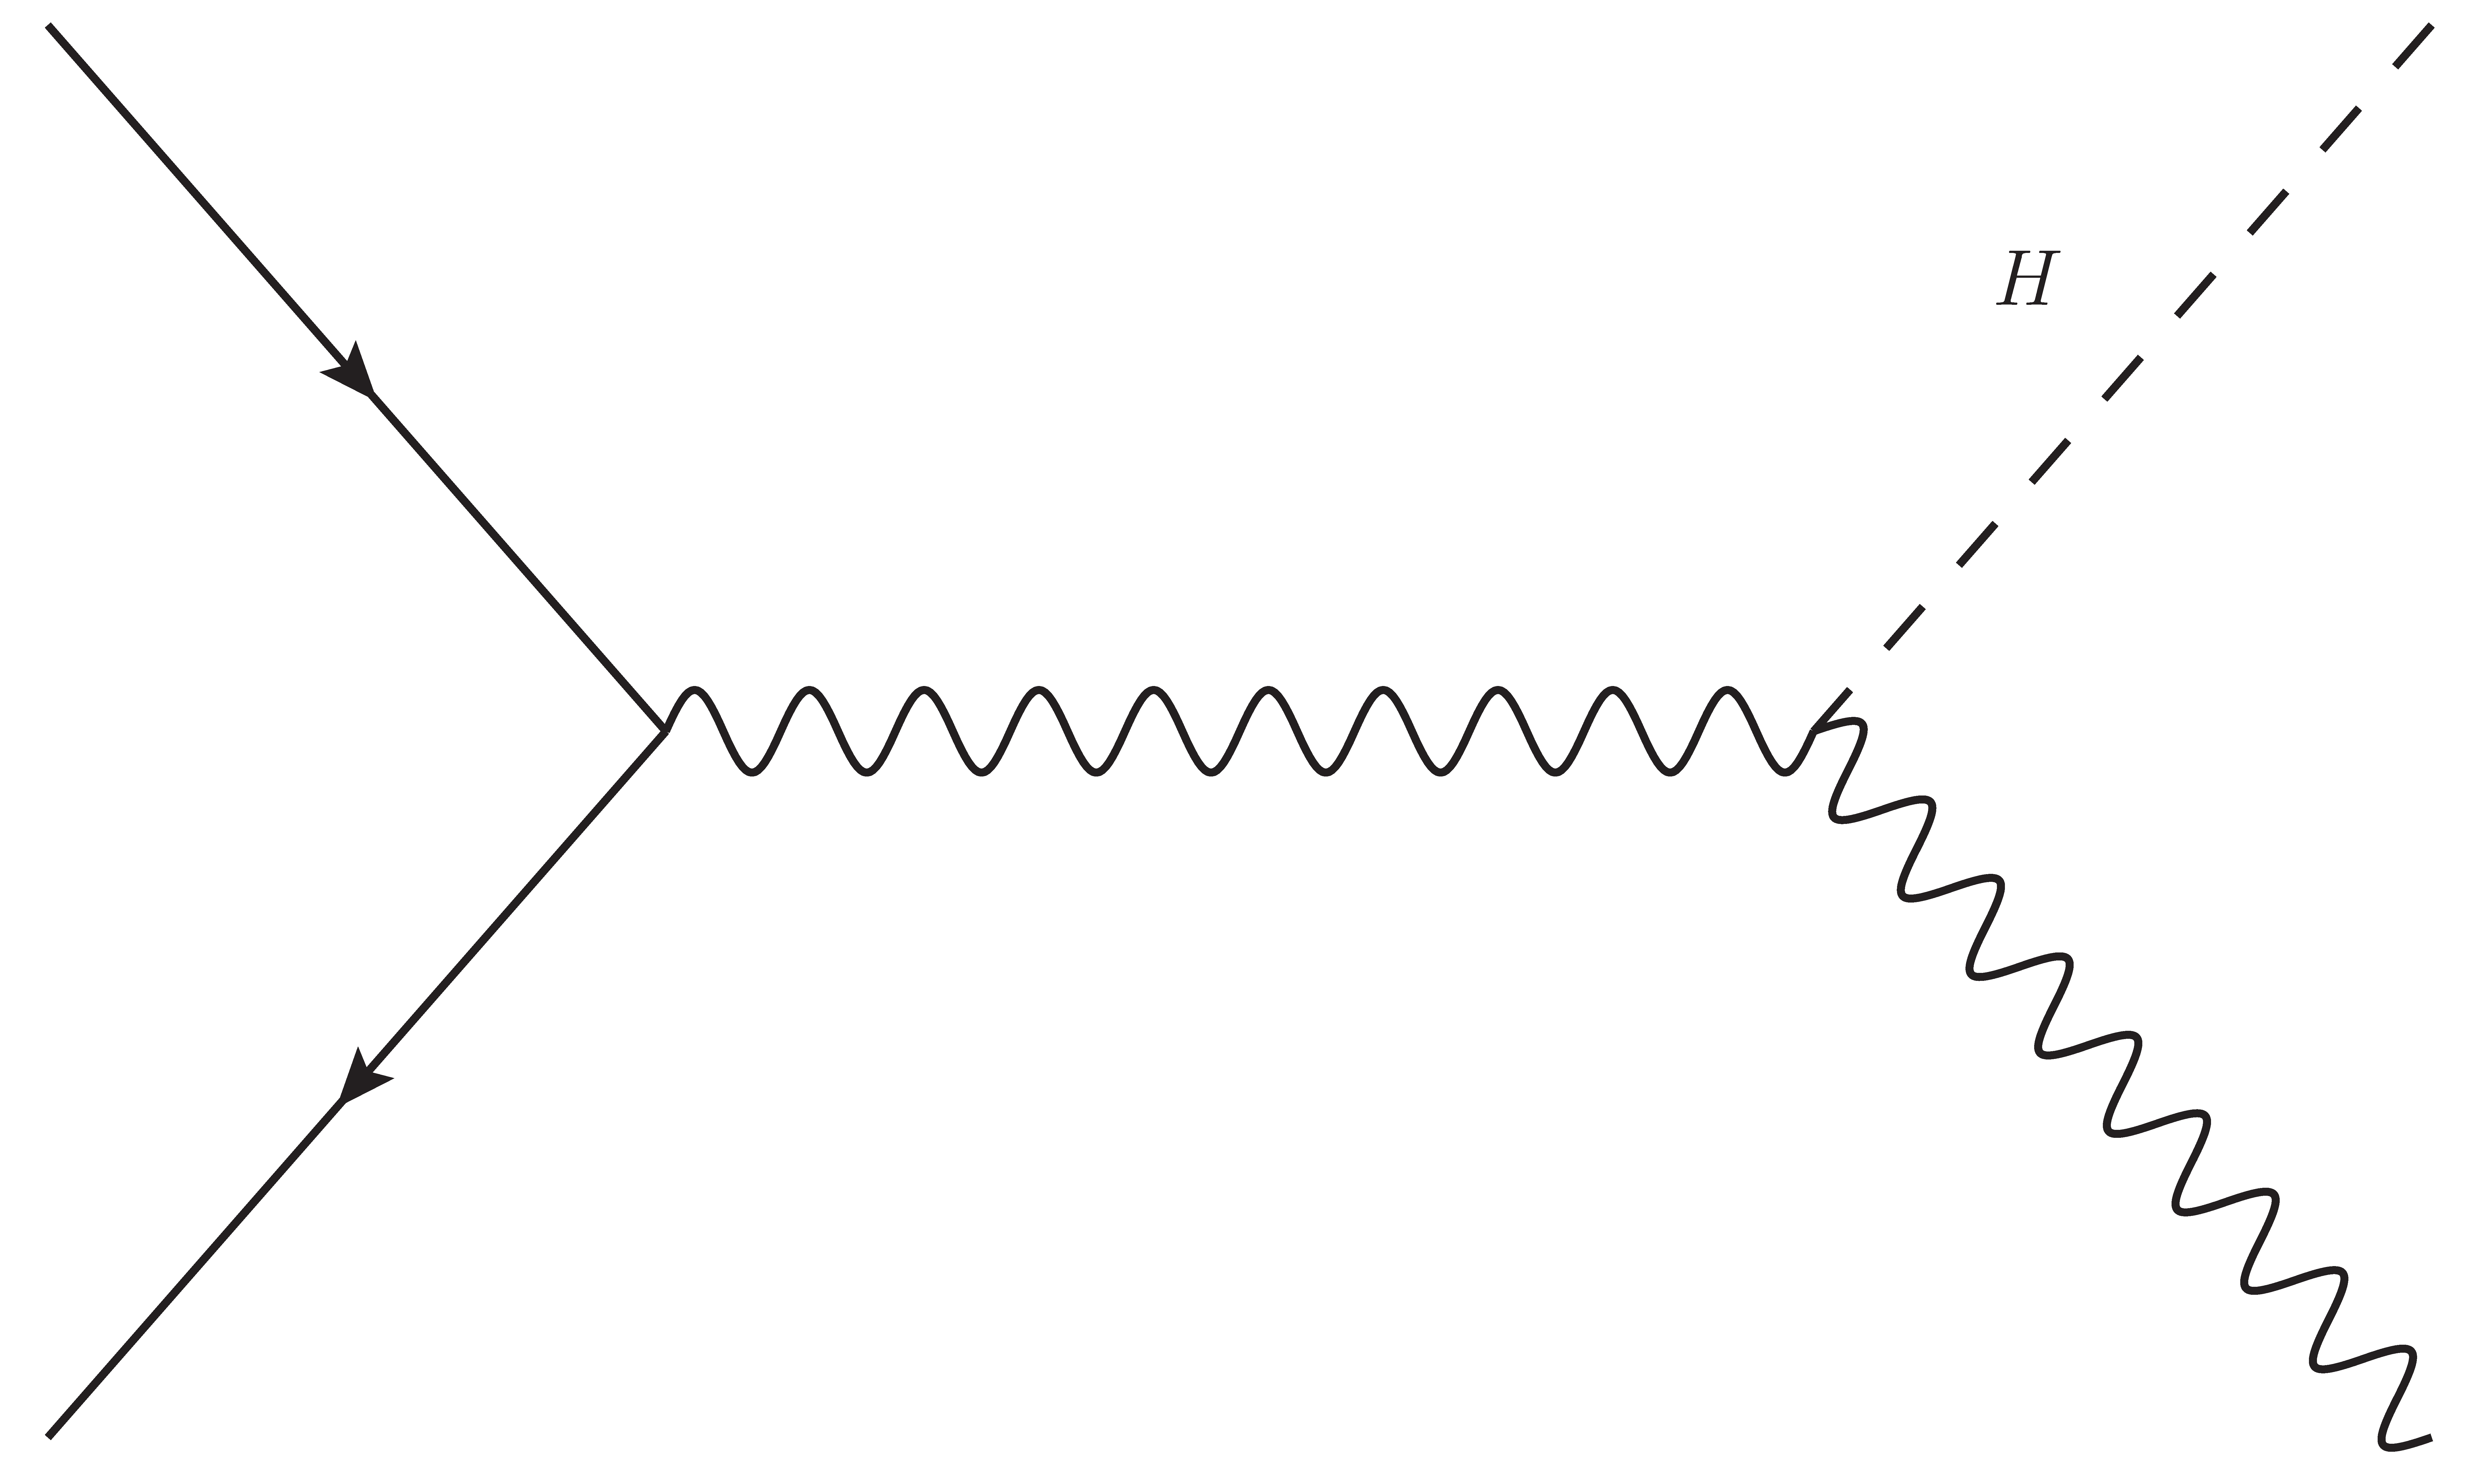
\includegraphics[width=0.42\textwidth, height=4cm]{figs/Higgstrahlung.png}
    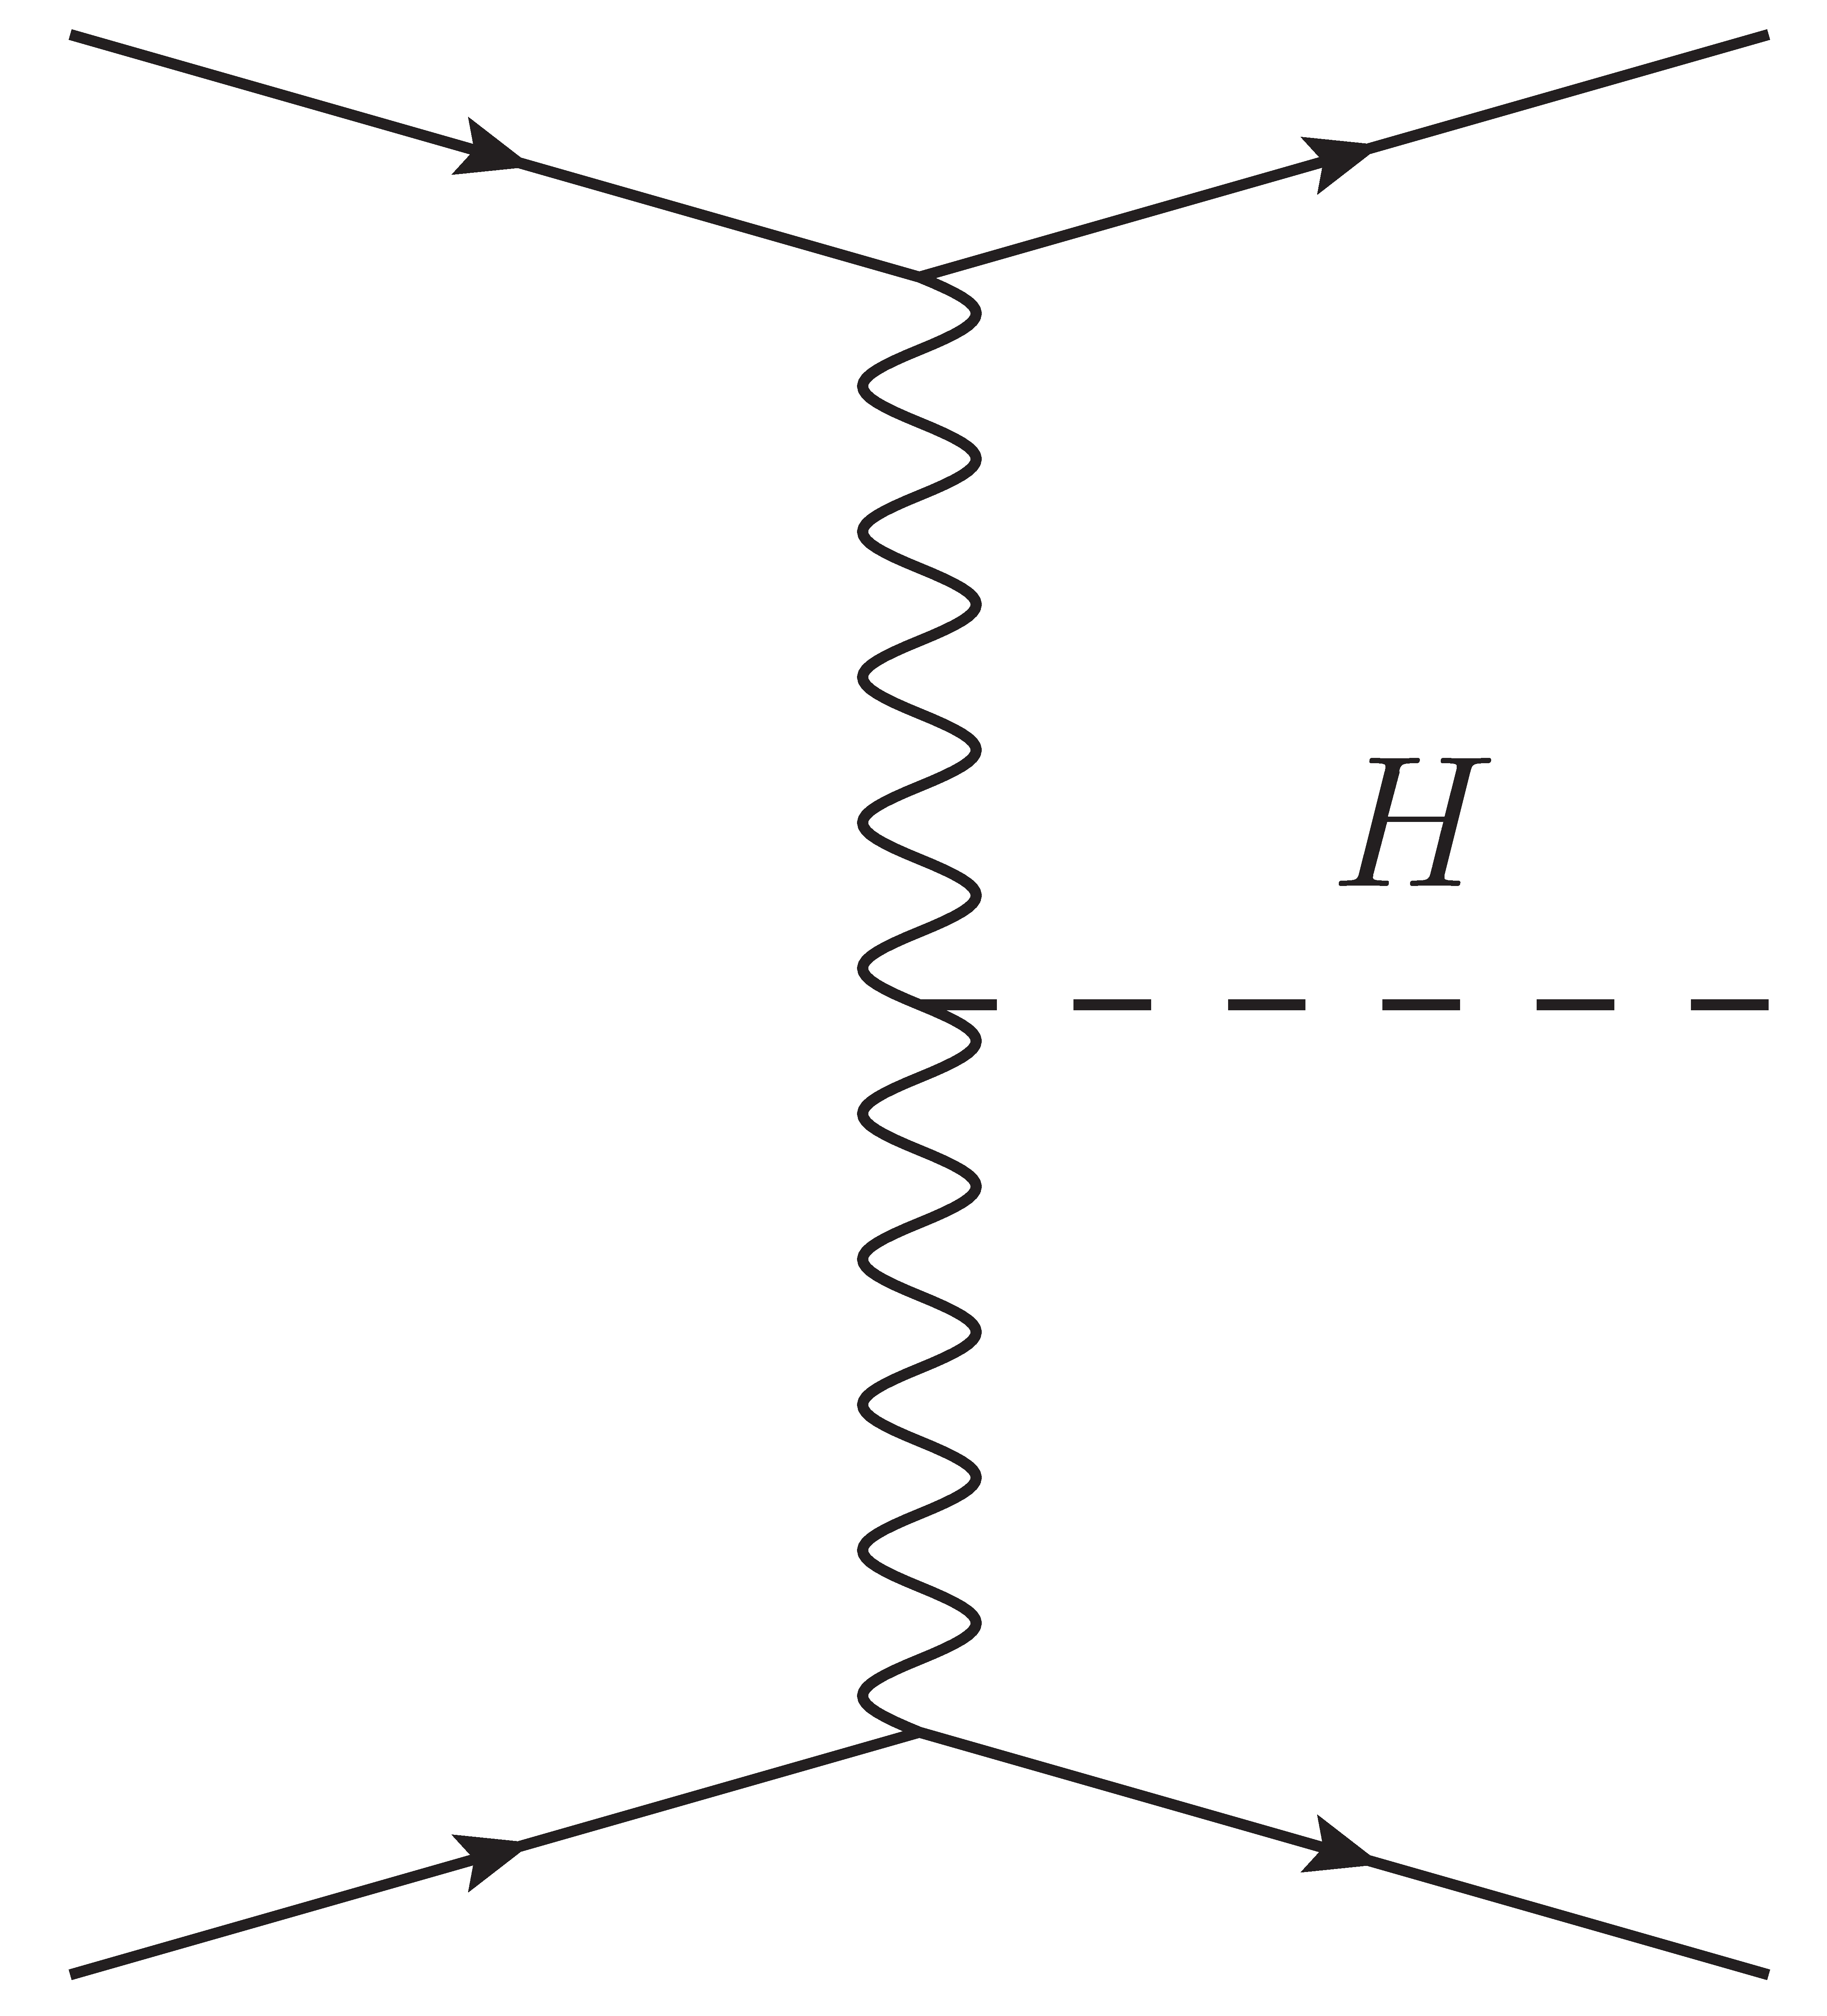
\includegraphics[scale=0.45]{figs/VBF_H.png}
    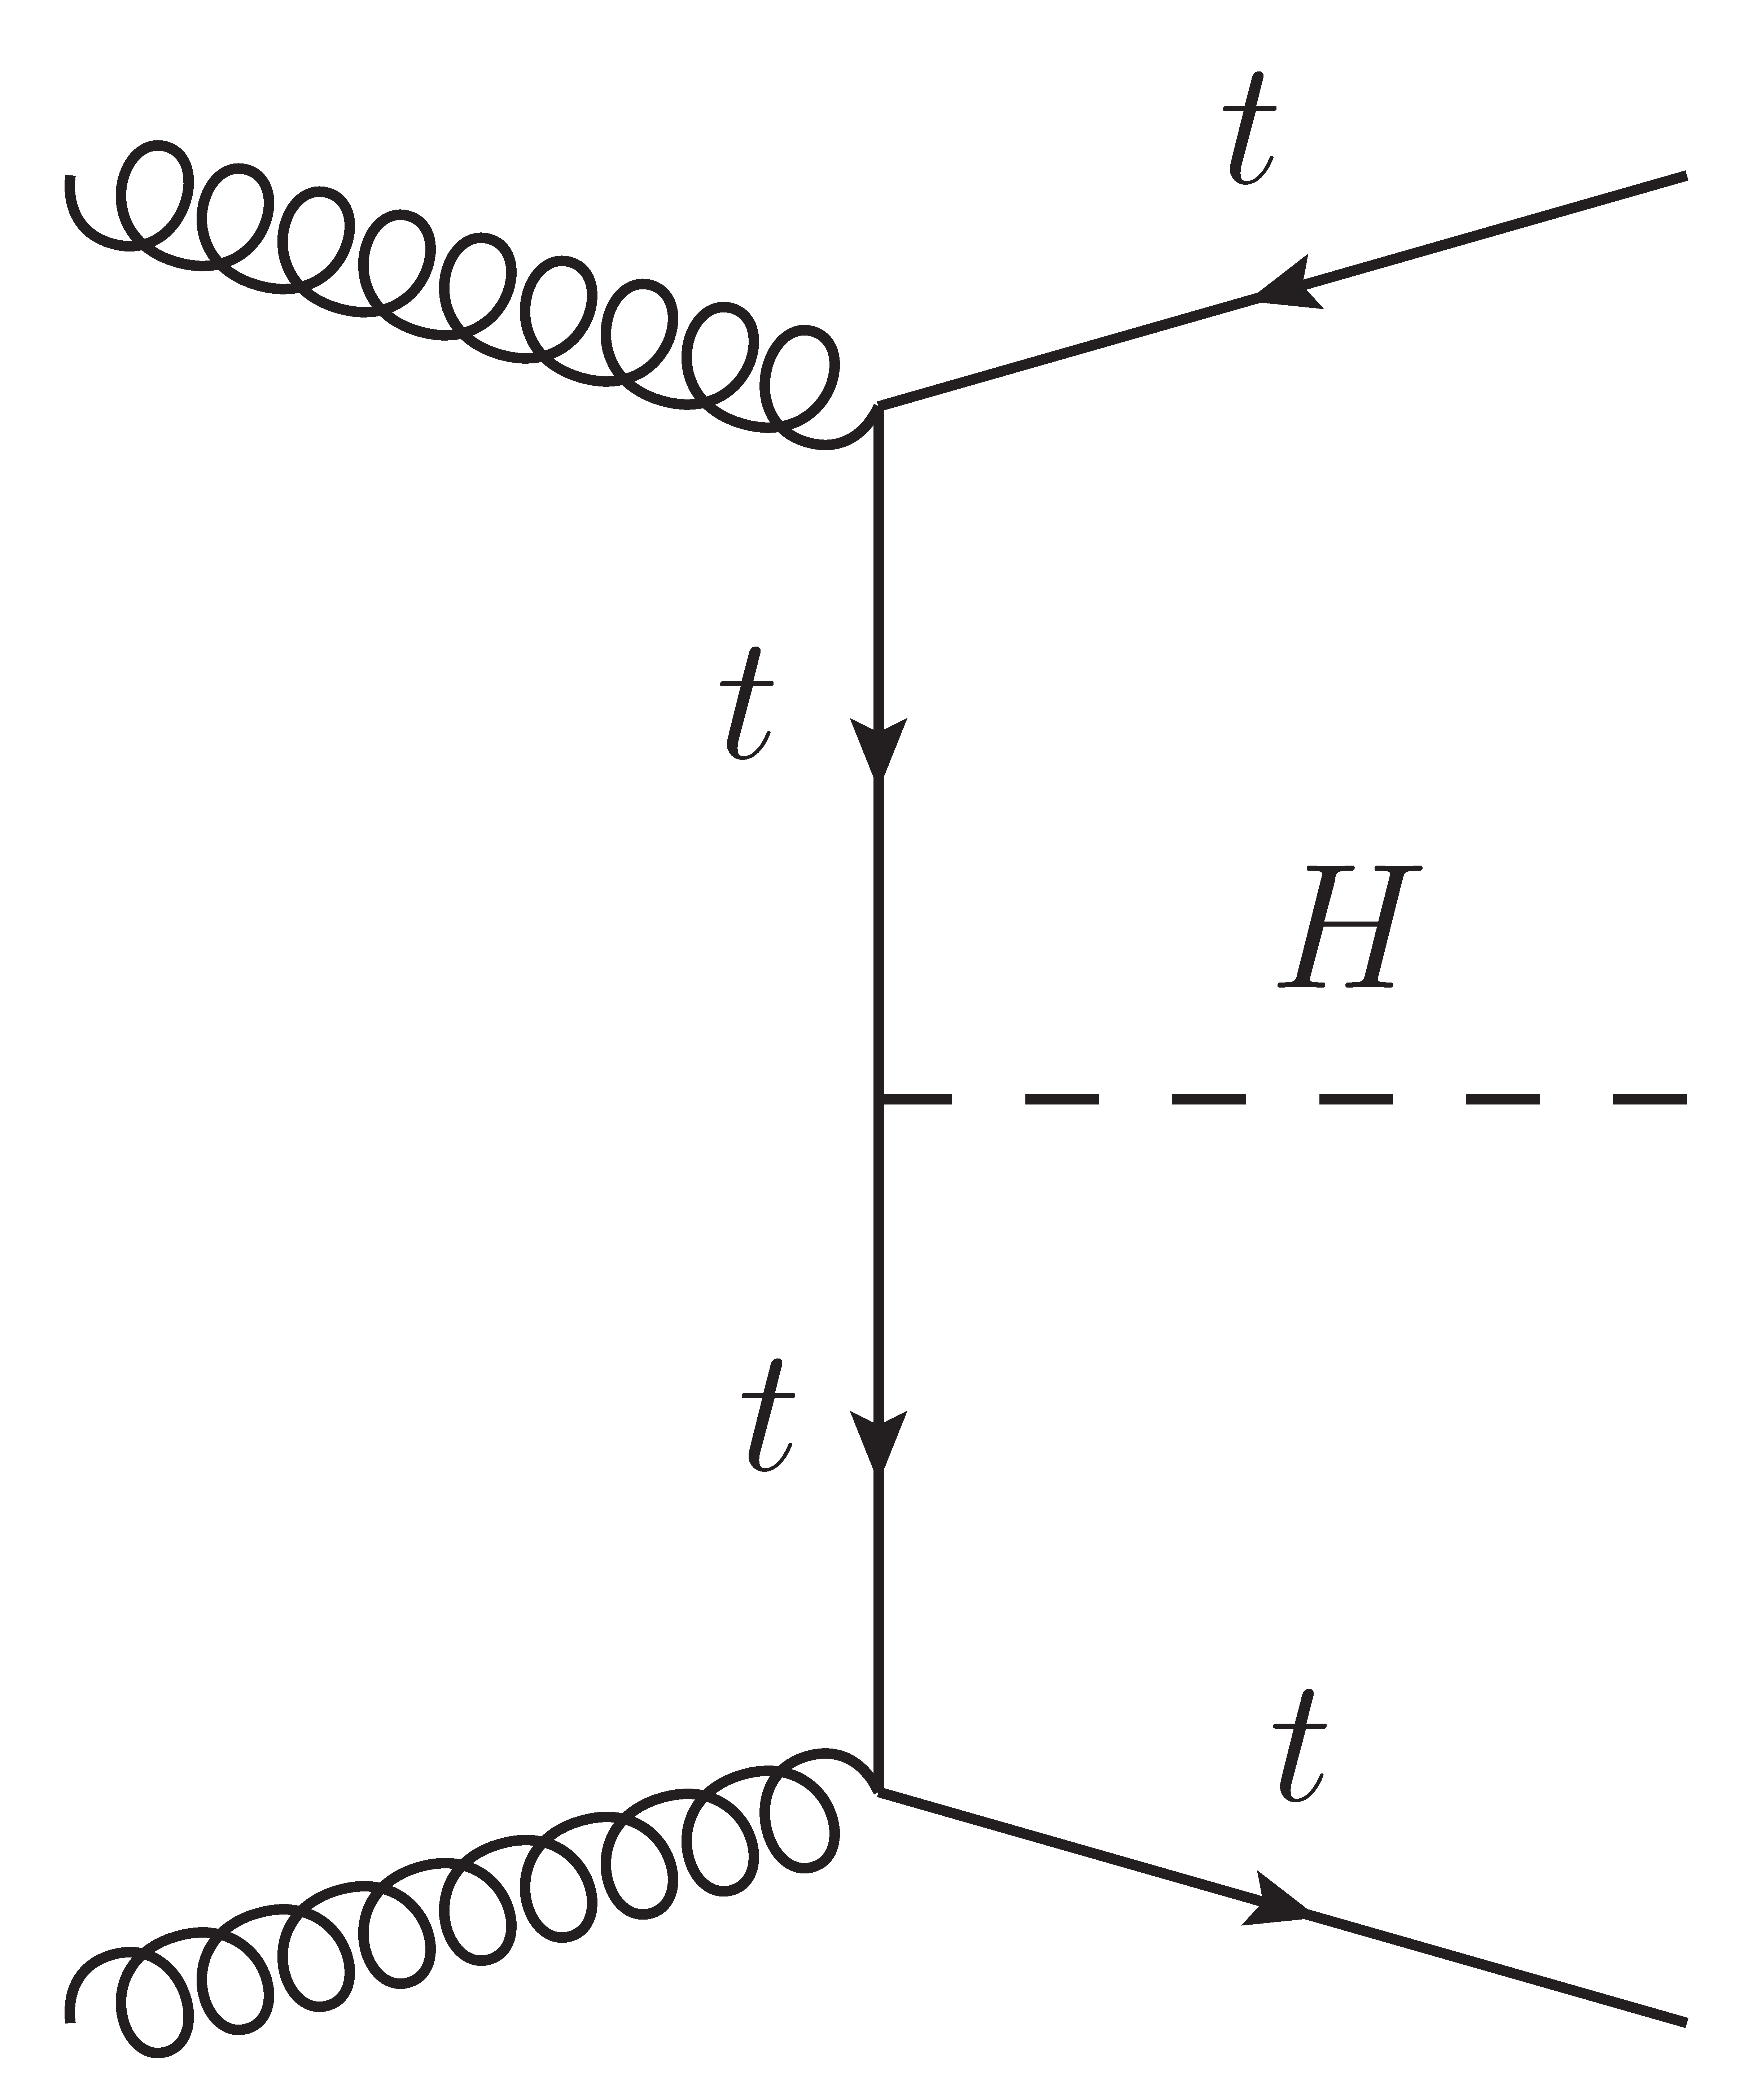
\includegraphics[scale=0.45]{figs/QuarkF_H.png}
    \caption{Higgs production Feynman diagrams for proton-proton collisions: gluon fusion [left-up], Higgsstrahlung [right-up], vector boson fusion [left-down] and quark fusion [right-down]}
    \label{fig:HiggsProd}
  \end{center}
\end{figure}

All these processes have different contributions to the Higgs boson production cross section. In figure~\ref{fig:HiggsProdXS}, the cross section of Higgs boson production for a Higgs mass of 125 GeV/$c^{2}$ for different center of mass energies at LHC is shown (\cite{Dittmaier:2011ti, Dittmaier:2012vm, Heinemeyer:2013tqa, HIGGSXSWG}). The dominant production is the gluon fusion, all the other processes cross sections are at least one order of magnitude smaller. The total Higgs boson production cross section at LHC can be seen in figure~\ref{fig:TotalHiggsXS}, taken from~\cite{Dittmaier:2011ti, Dittmaier:2012vm, Heinemeyer:2013tqa, HIGGSXSWG}, as function of Higgs mass and for different center of mass energies. At run 1 energies, 7-8 TeV, the total production cross section is about 20 pb, while at 13 TeV it will be 2.3 times higher, reaching $\sim$50 pb. 

\begin{figure}[!Hhtbp]
  \begin{center}
    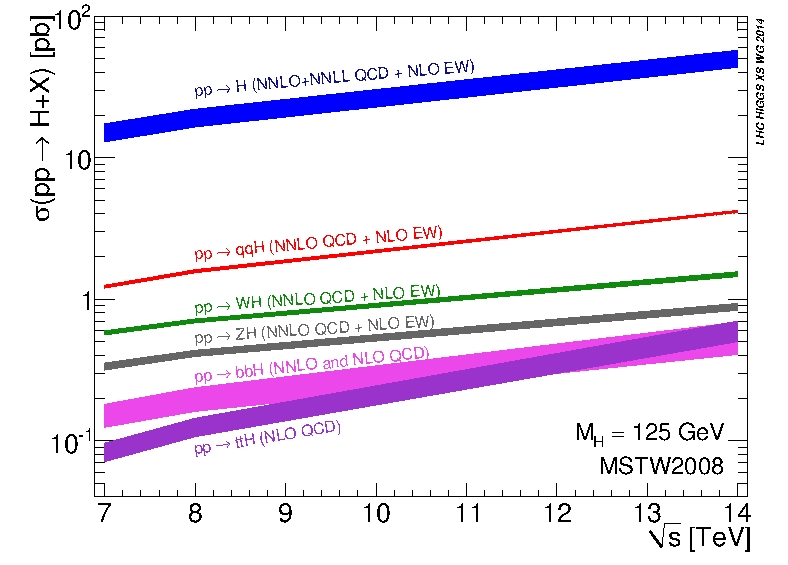
\includegraphics[width=0.6\textwidth]{figs/7-14_Higgs_xsec.jpg}
    \caption{Higgs theoretical production cross section as function of center of mass energy, for a Higgs boson with a mass of 125 GeV/$c^{2}$.}
    \label{fig:HiggsProdXS}
  \end{center}
\end{figure}

\begin{figure}[!Hhtbp]
  \begin{center}
    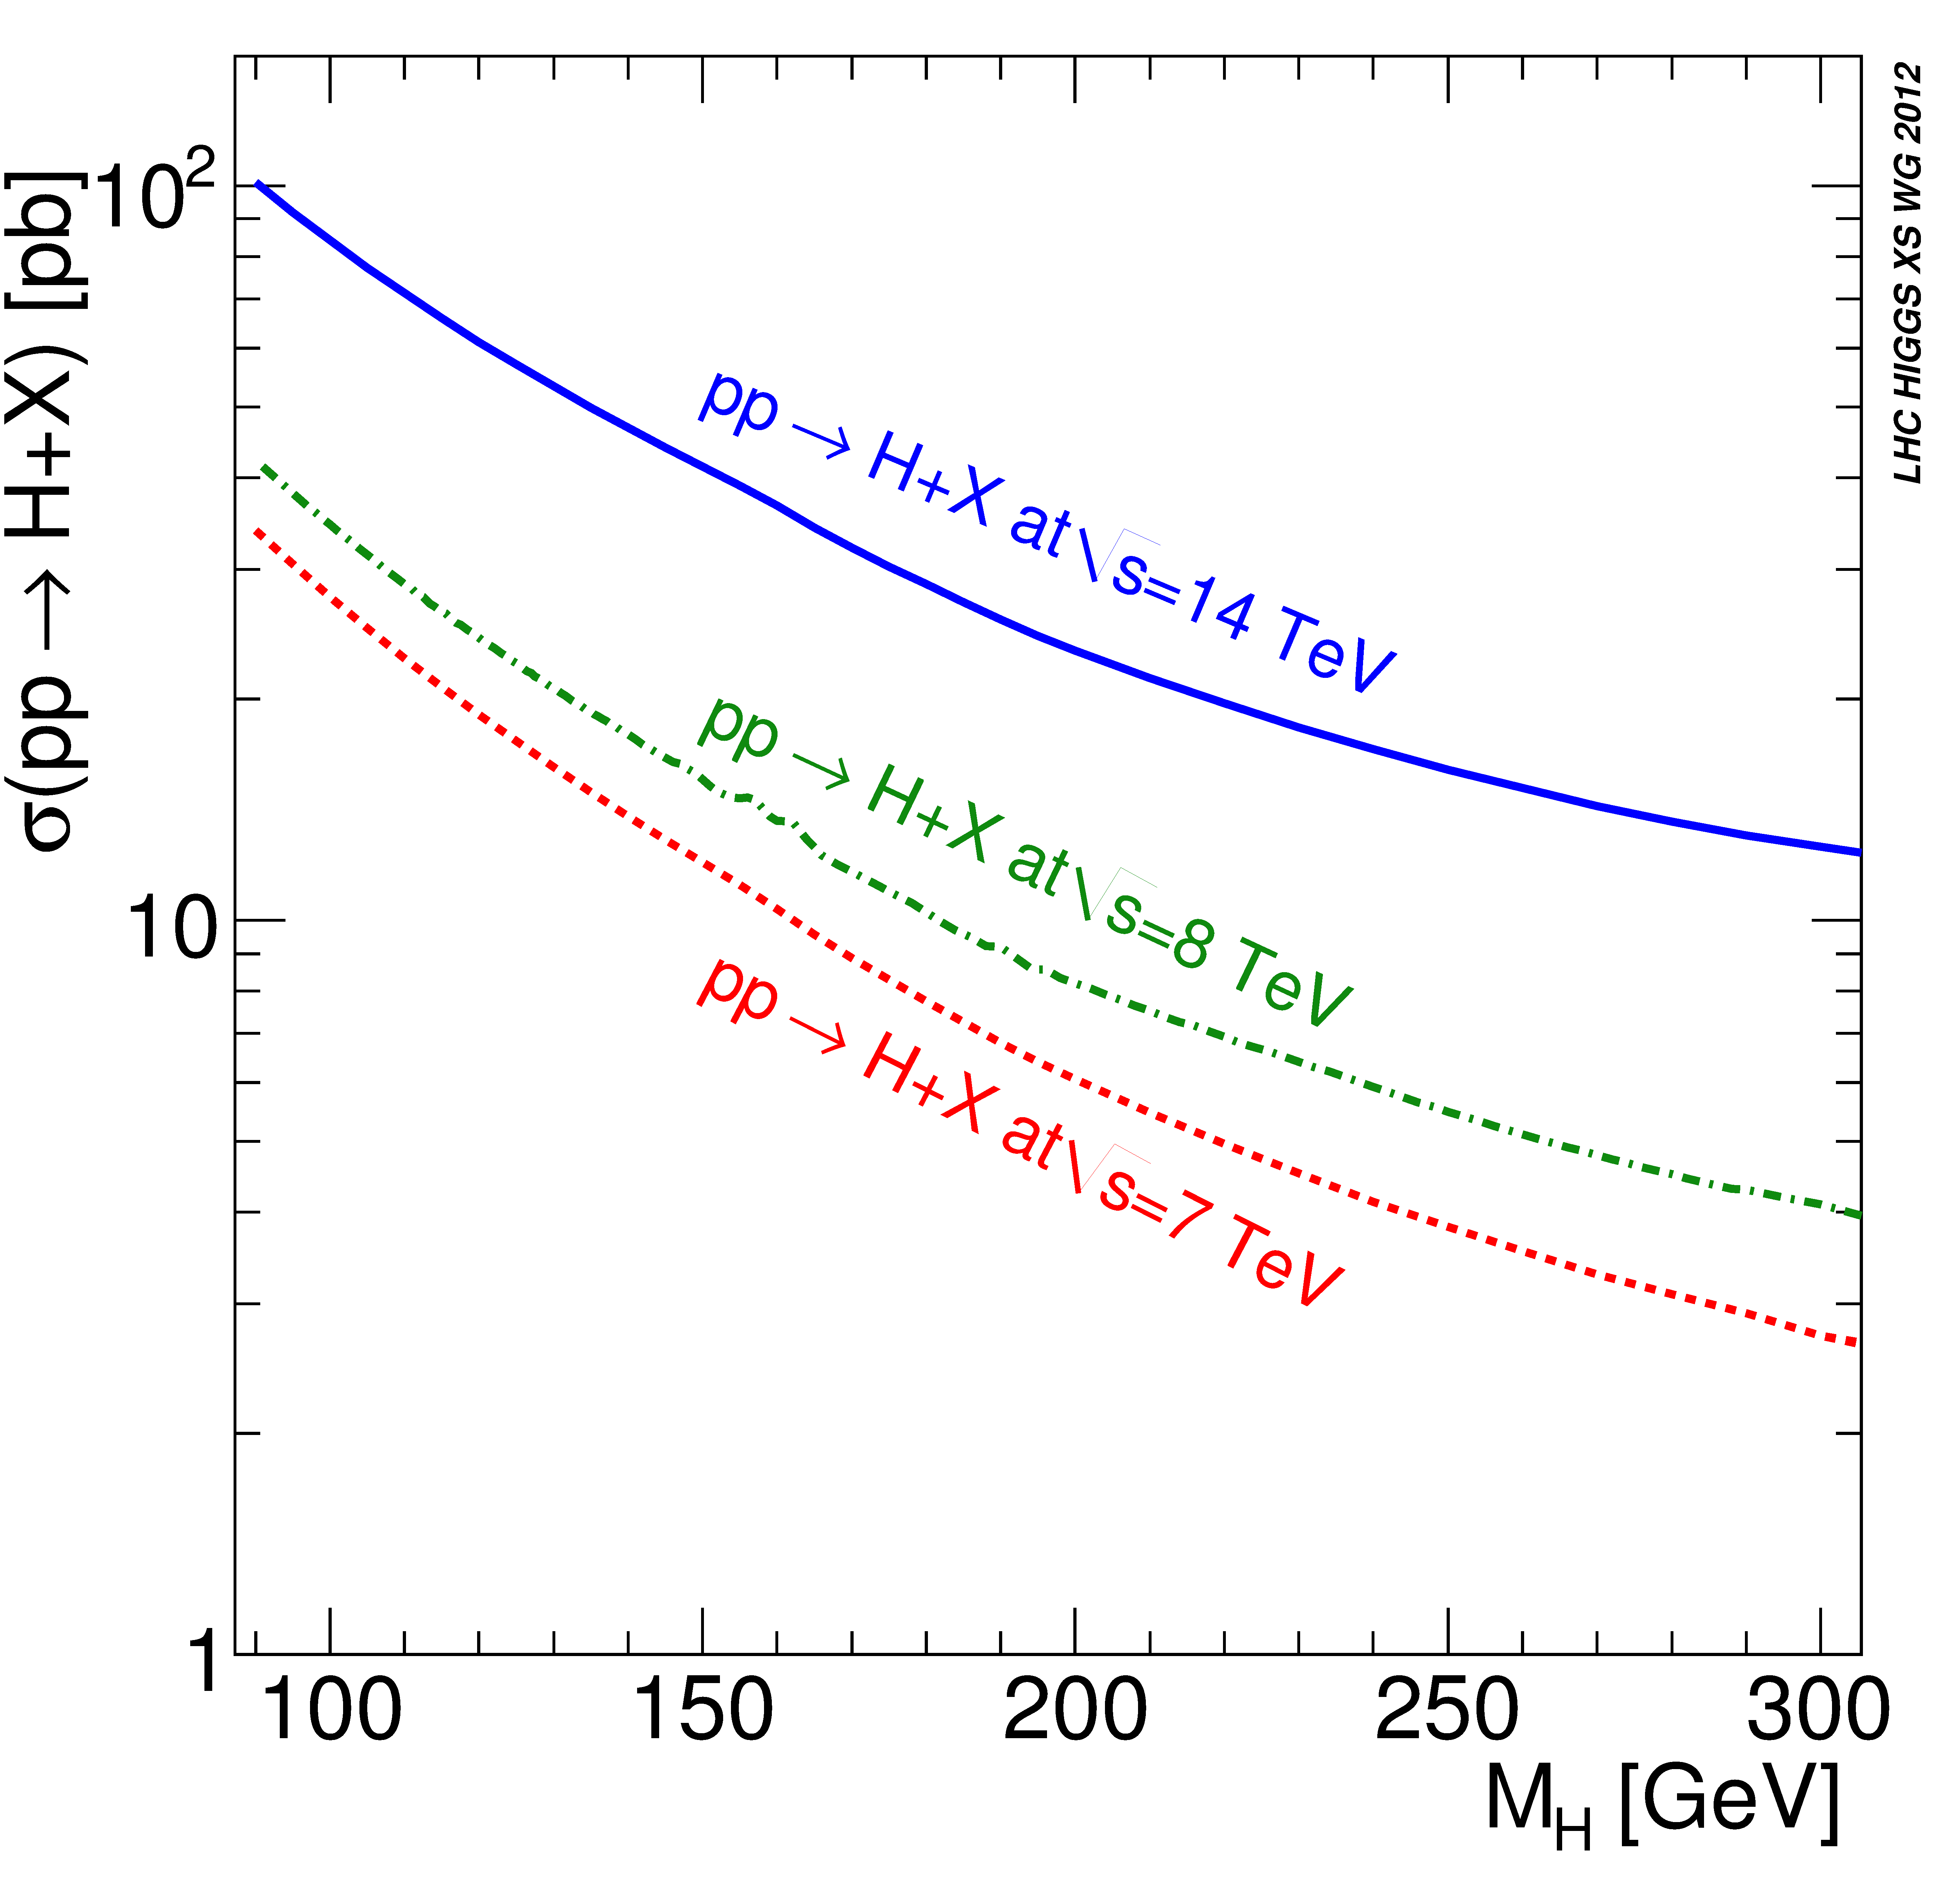
\includegraphics[width=0.6\textwidth]{figs/totalXS_LM.png}
    \caption{Total Higgs production cross section as function of Higgs mass for different center of mass of proton-proton collisions.}
    \label{fig:TotalHiggsXS}
  \end{center}
\end{figure}

%\begin{TOINCLUDE}Plots of cross section of Higgs production as function of center of mass energy; Feynman diagrams for Higgs production\end{TOINCLUDE}

\subsection{Higgs decay channels}

As the Higgs boson couples to all particles in the SM it can decay of several ways. Figure~\ref{fig:HiggsBrs}, taken from~\cite{Dittmaier:2011ti, Dittmaier:2012vm, Heinemeyer:2013tqa, HIGGSXSWG}, shows the branching ratios of the decay channels of the Higgs boson as function of the Higgs mass. The highest branching ratio corresponds to its decay to two b-quarks. This channels is difficult to observe due to the high QCD and \ttbar~backgrounds, however it gives the highest expected number of events as more than the half of Higgs bosons produced at LHC decay into \bbbar~final state. The Higgs decay to $ZZ$ is an important channel because it has a high branching ratio and one of its final states is 4 leptons, a very clean final state (low background rate), called the golden channel. Finally, even if the diphoton channel has specially low branching ratio it is very clean in terms of photon identification and resolution. In the search that is going to be presented in chapter~\ref{chap:search}, the Higgs boson is going to be looked for in the \bbbar~decay. In figure~\ref{fig:HiggsDecays} the Feynman diagrams of the discussed decay channels are presented.

\begin{figure}[!Hhtbp]
  \begin{center}
    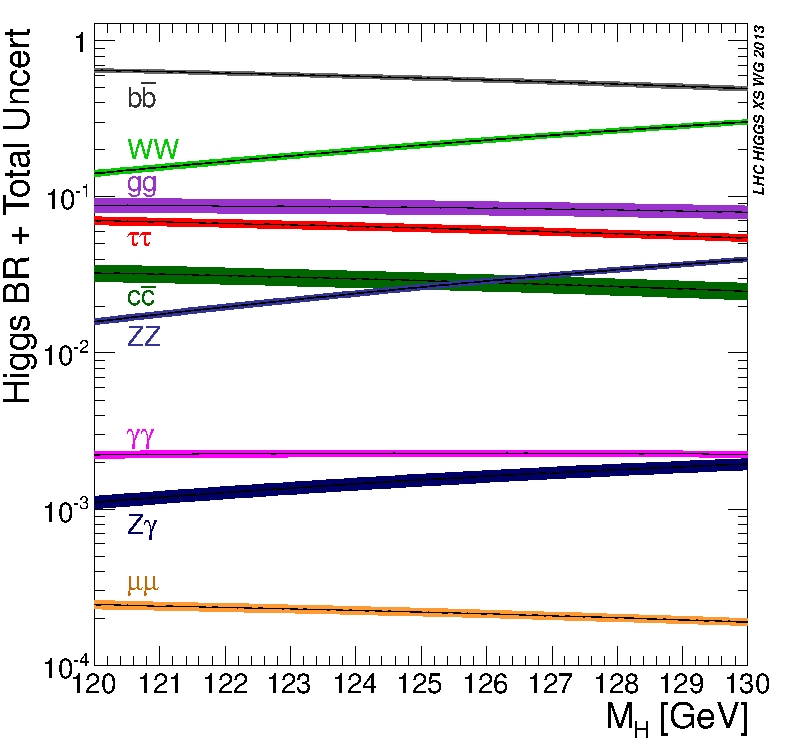
\includegraphics[width=0.8\textwidth]{figs/Higgs_BR_120-130.jpg}
    \caption{Higgs decay branching ratios as function of Higgs mass.}
    \label{fig:HiggsBrs}
  \end{center}
\end{figure}

\begin{figure}[!Hhtbp]
  \begin{center}
    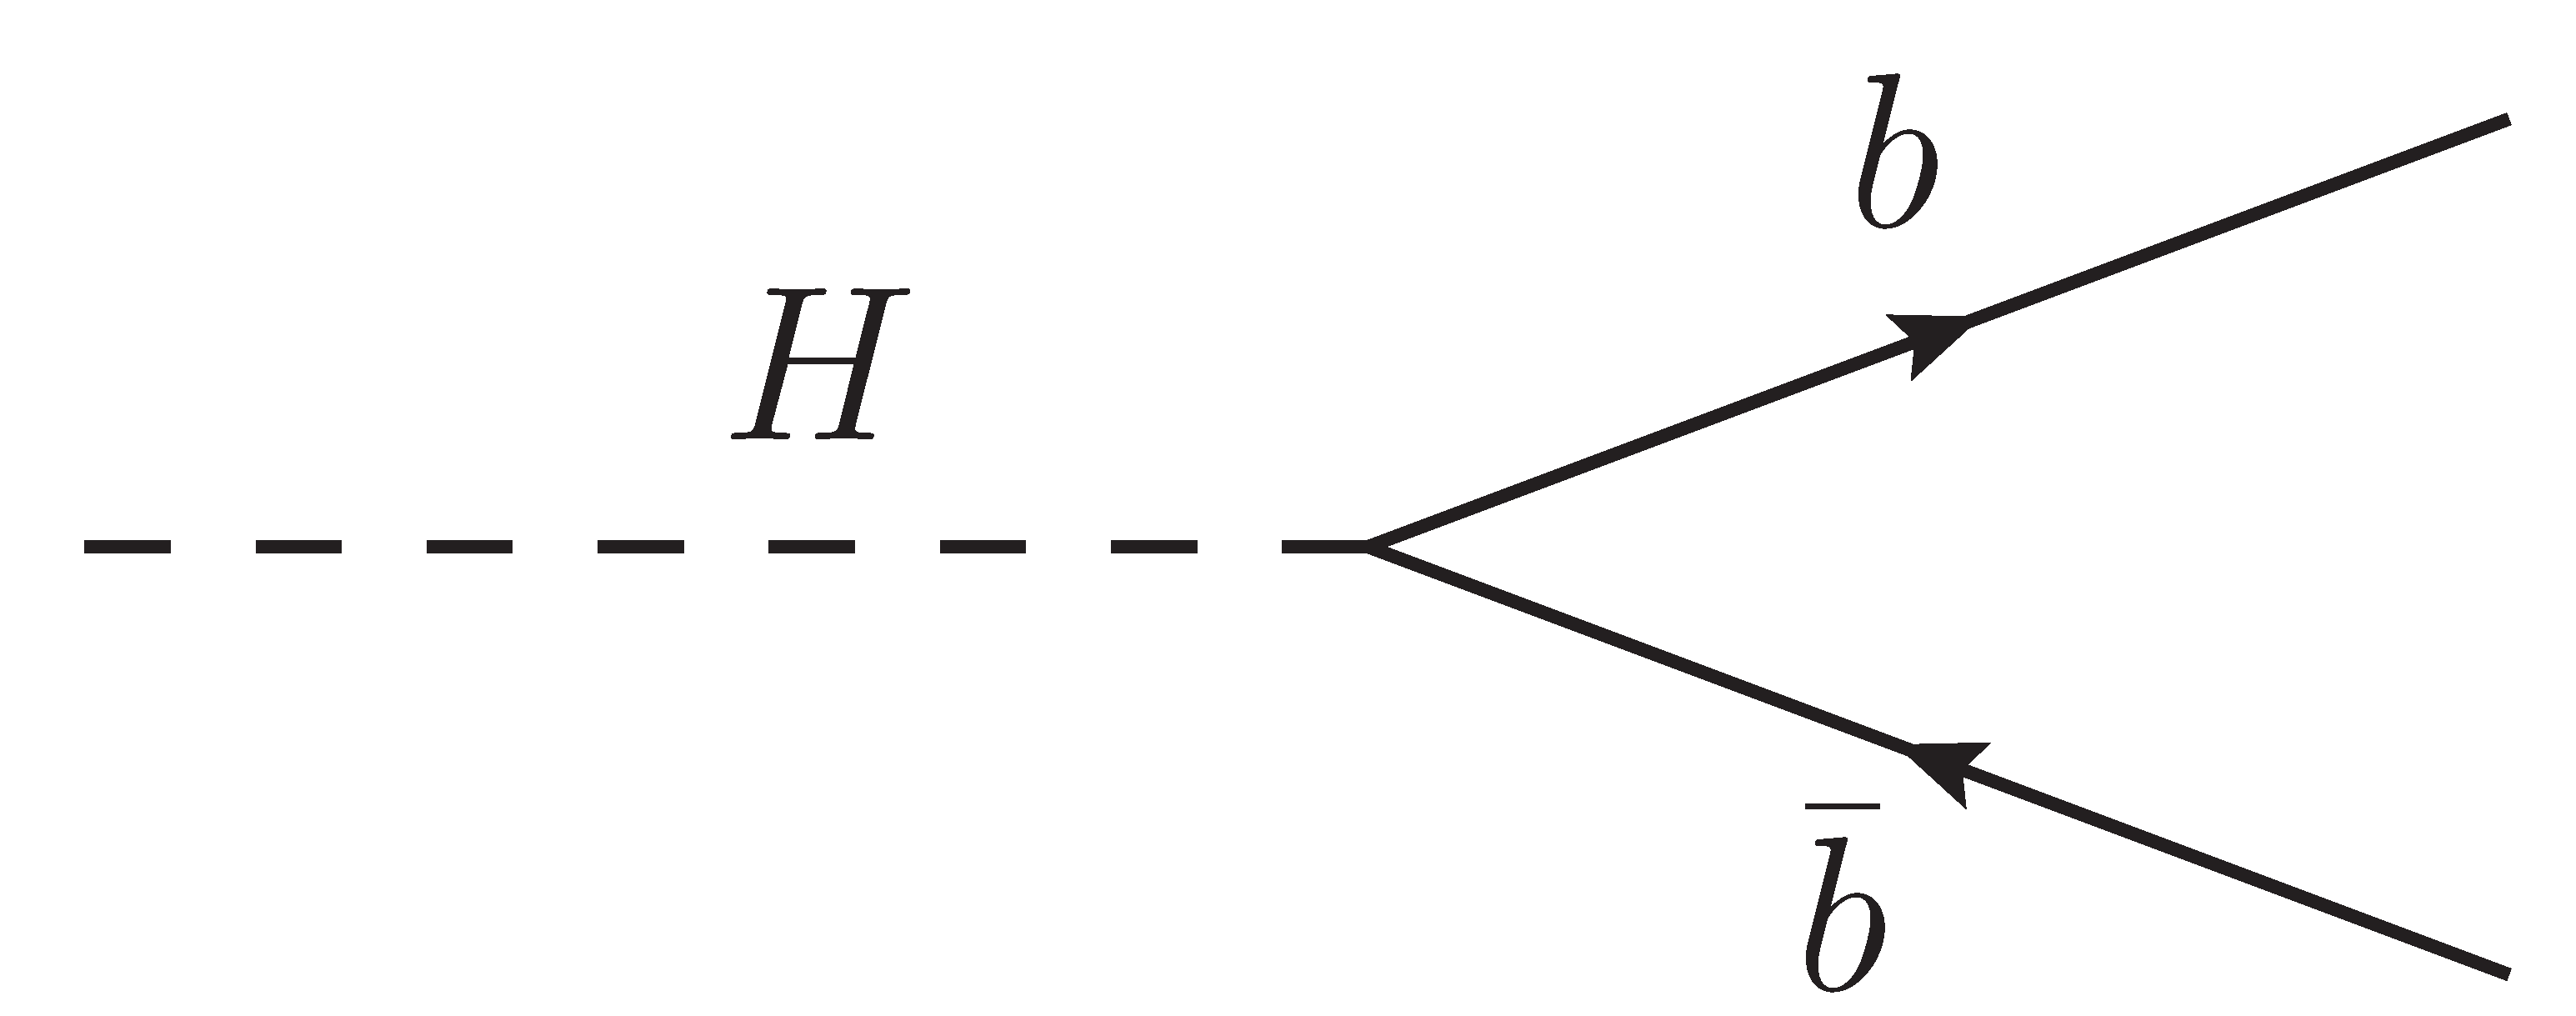
\includegraphics[width=0.3\textwidth]{figs/BB_H.png}
    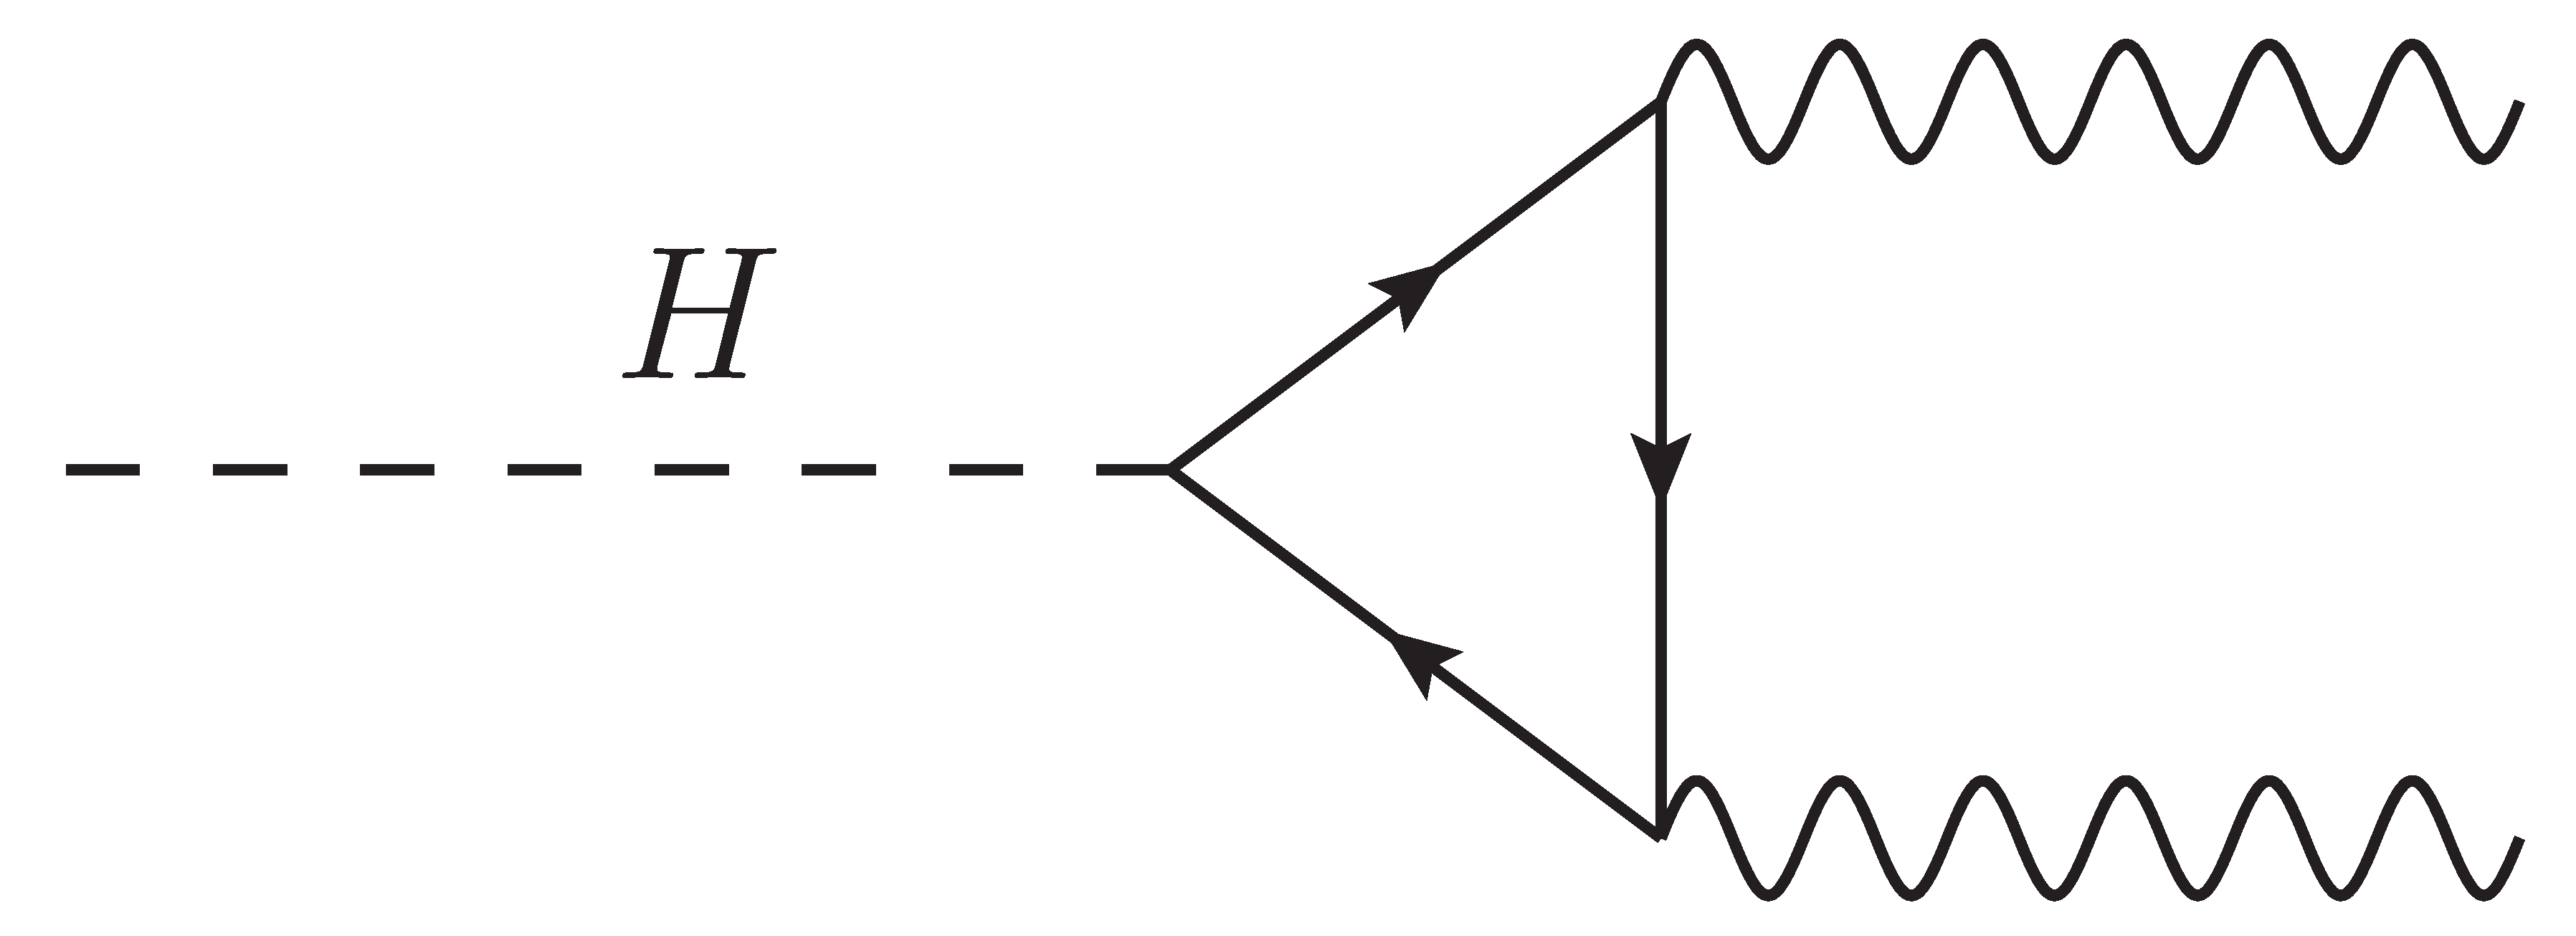
\includegraphics[width=0.3\textwidth]{figs/Diphoton_H.png}
    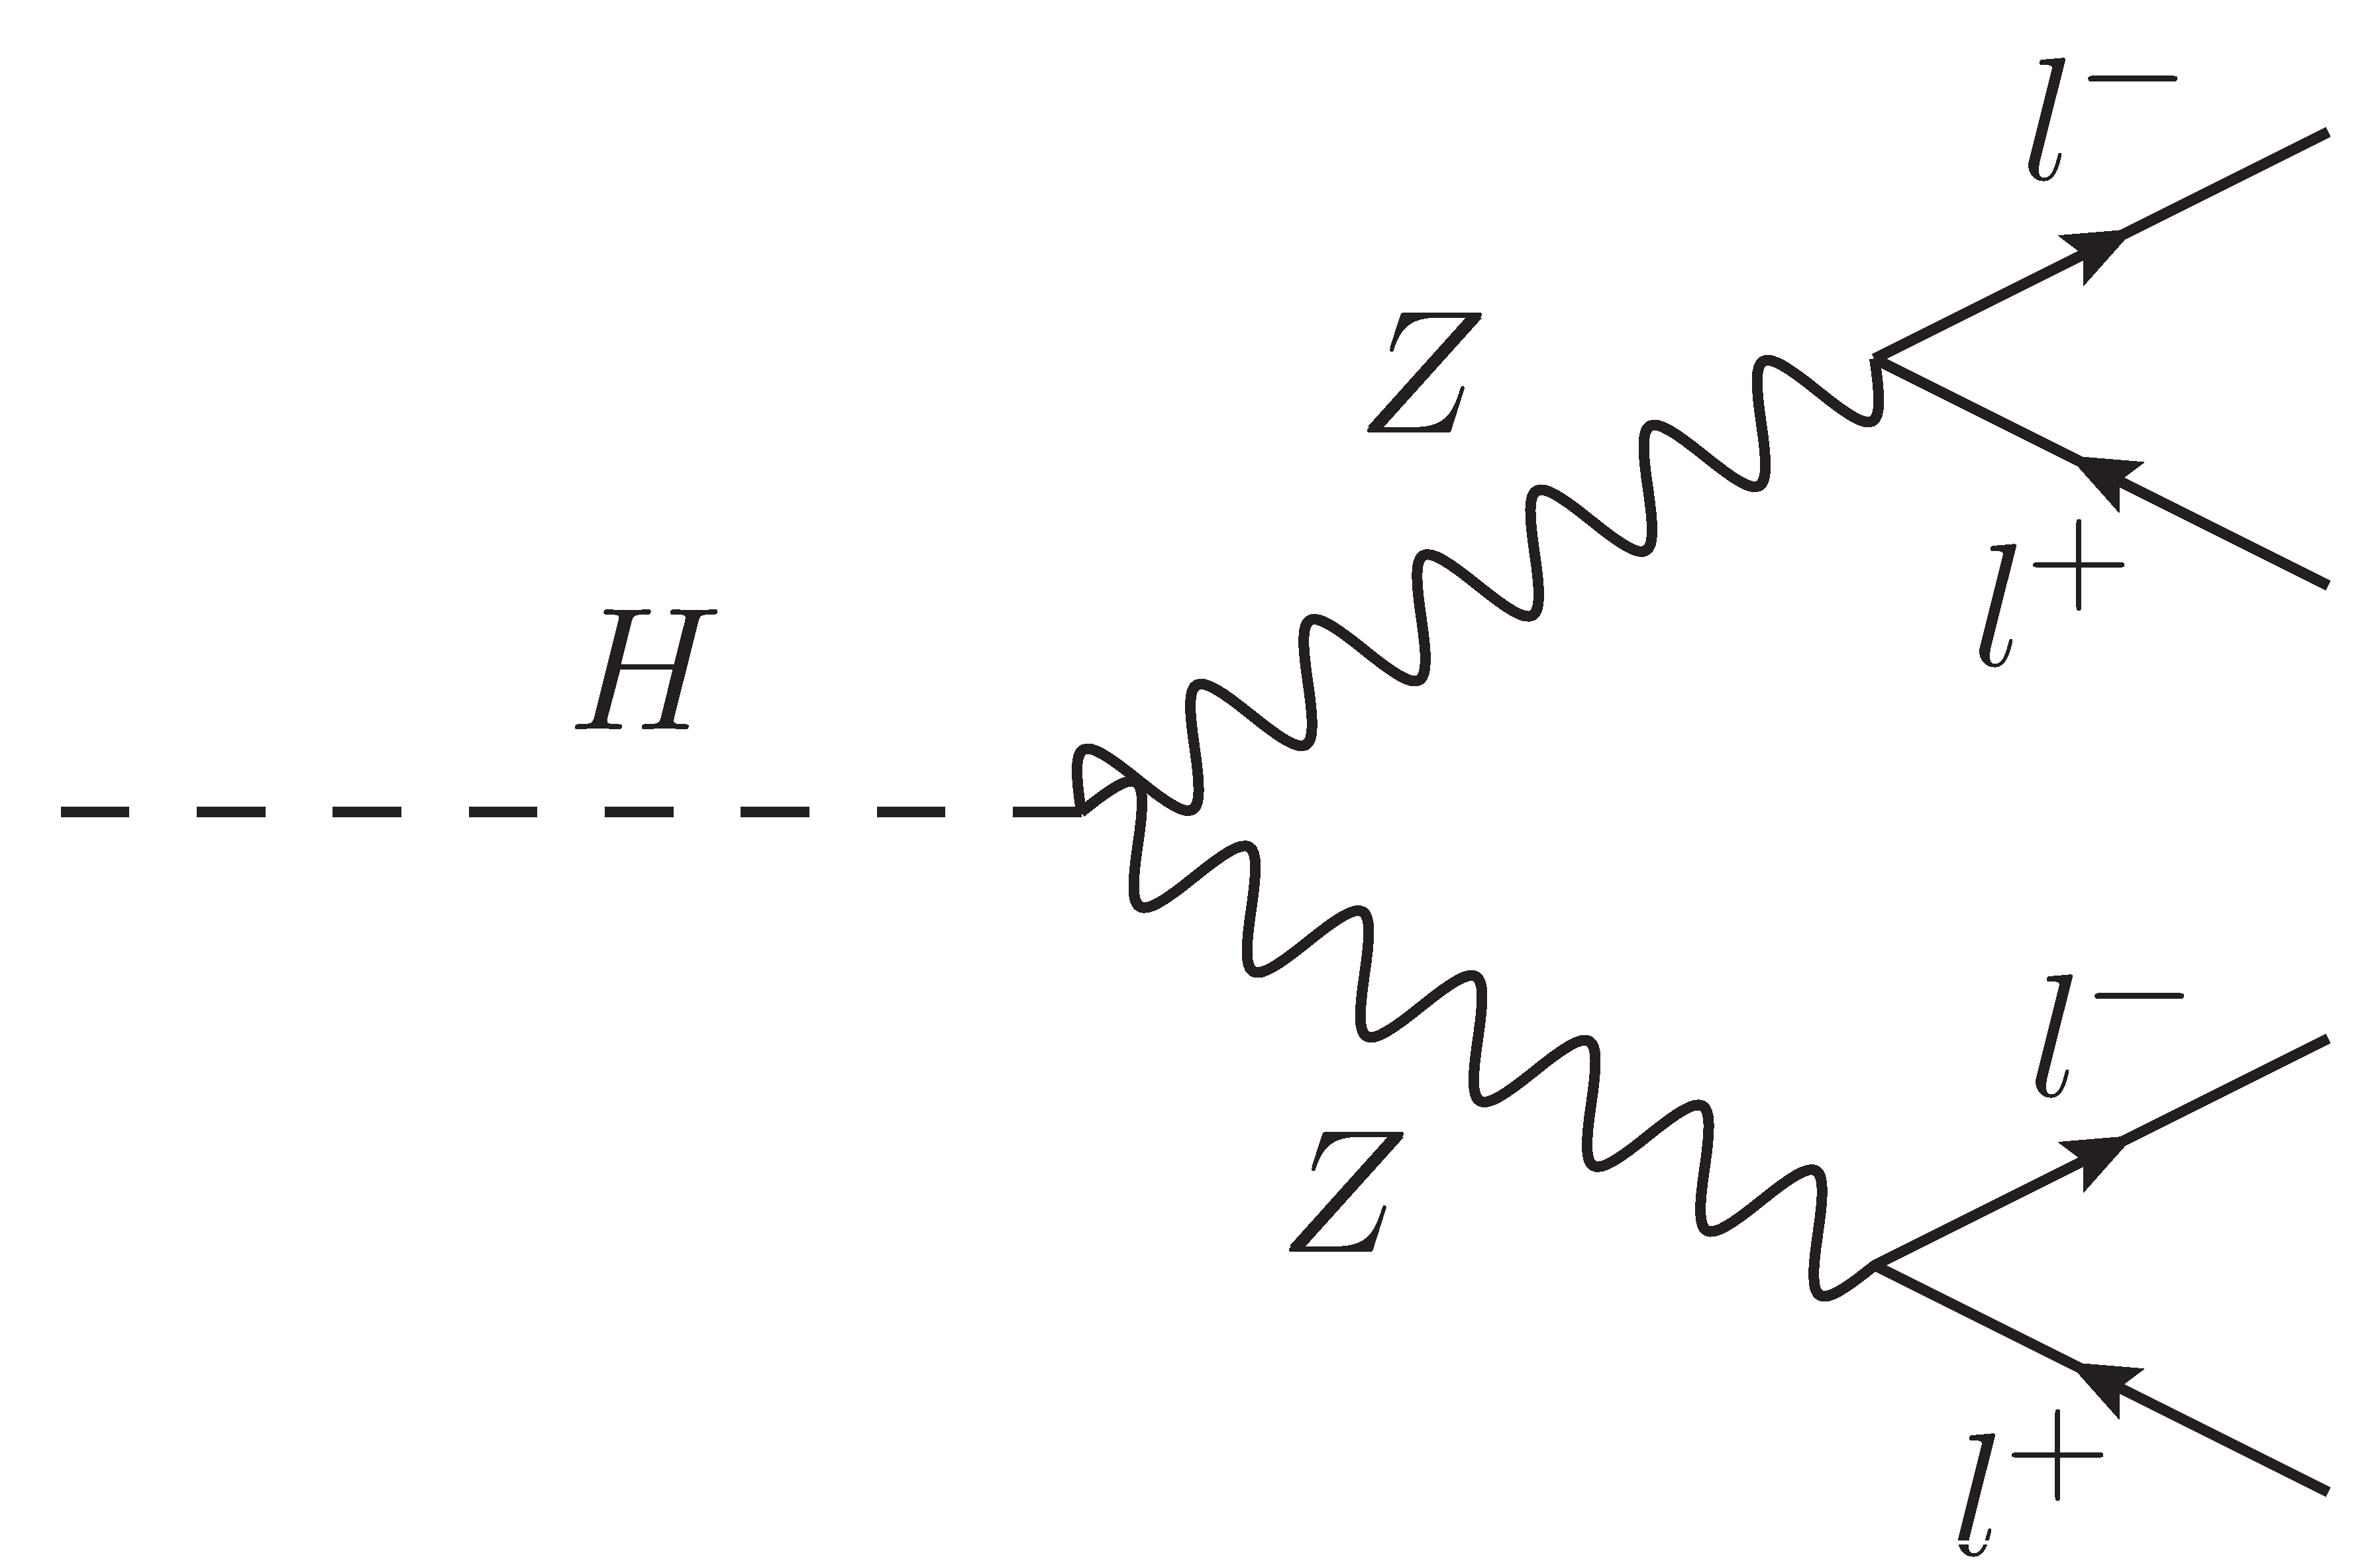
\includegraphics[width=0.3\textwidth]{figs/Golden_H.png}
    \caption{Feynman diagrams of Higgs decay: $b\bar{b}$ [left], diphoton [center] and golden channels [right]}
    \label{fig:HiggsDecays}
  \end{center}
\end{figure}
%\begin{TOINCLUDE}Plot on possible decay channels and branching ratios to each channel; Feynman diagram for each golden bb and diphoton channels\end{TOINCLUDE}

\subsection{Mass and width of Higgs boson}

The 4th of July of 2012 was announced the discovery of a Higgs boson like particle at LHC by ATLAS and CMS collaborations. It was discovered in several decay modes, but the most significant result was coming from the combination of results in all analyzed channels. Such searches have been refined during last years, consolidating the discovery. 

To measure the mass of the Higgs boson, diphoton and golden channel analyses have been combined between ATLAS and CMS~\cite{Aad:2015zhl}. The found value by the combination is $m_{H}=125.09\pm 0.24$. Combination and separated ATLAS and CMS results are shown in figure~\ref{fig:HiggsMass} (from~\cite{Aad:2015zhl,CMS:2014ega,ATLAS-CONF-2015-007}). In the same figure are shown the results, in terms of measured cross section, of all analyses done by CMS looking for a Higgs boson in different final states. The results are compatible with SM expectations.

\begin{figure}[!Hhtbp]
  \begin{center}
    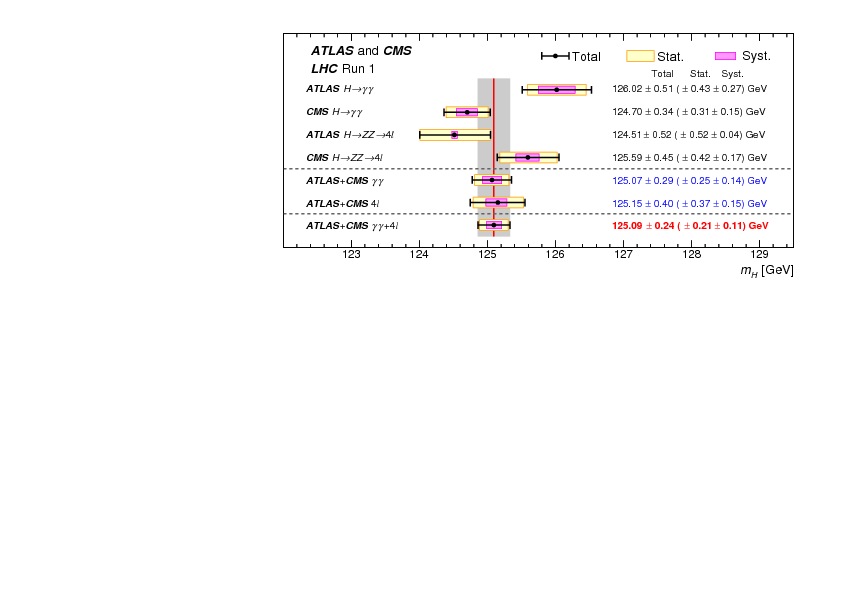
\includegraphics[trim=10cm 7cm 1cm 1cm, clip=true, width=0.8\textwidth]{figs/LHC_combined_obs_unblind_summary_a1_final.png}
    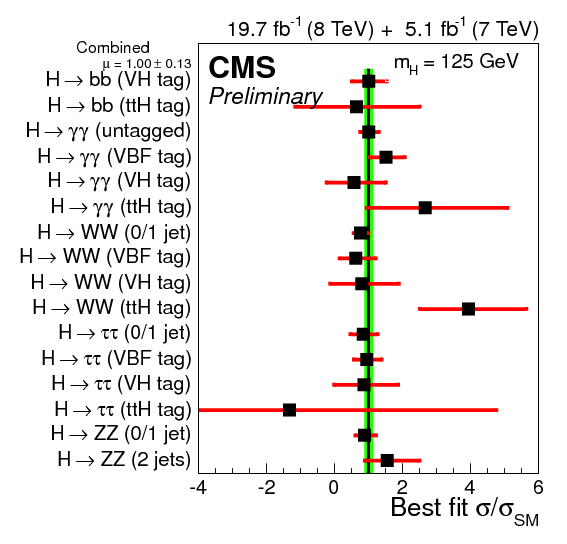
\includegraphics[width=0.55\textwidth]{figs/sqr_mlz_ccc_mH125.png}
    \includegraphics[width=0.4\textwidth]{figs/ATLAS_HIGGS_mu_Summary.png}
    \caption{ATLAS and CMS combination of Higgs mass measurement [top] and $\sigma/\sigma_{SM}$ (measured cross section over theoretical SM cross section) for searches performed by ATLAS and CMS in different Higgs channels [bottom].}
    \label{fig:HiggsMass}
  \end{center}
\end{figure}

Whereas nowadays there are plenty of experimental results for the measurement of Higgs mass, measuring the Higgs width constitutes an important challenge. The predicted width from the SM is $\sim$4 MeV for a 125 GeV mass Higgs. Figure~\ref{fig:WidthHiggs} shows the width dependence on the Higgs mass, taken from~\cite{Dittmaier:2011ti, Dittmaier:2012vm, Heinemeyer:2013tqa, HIGGSXSWG}. In the figure is shown a method proposed by CMS collaboration using the golden channel to constraint Higgs width~\cite{CMS-PAS-HIG-14-002, Khachatryan:2014iha}. Such method put a limit of about 4.2 times the SM Higgs width ($\sim$20 MeV).

\begin{figure}[!Hhtbp]
  \begin{center}
    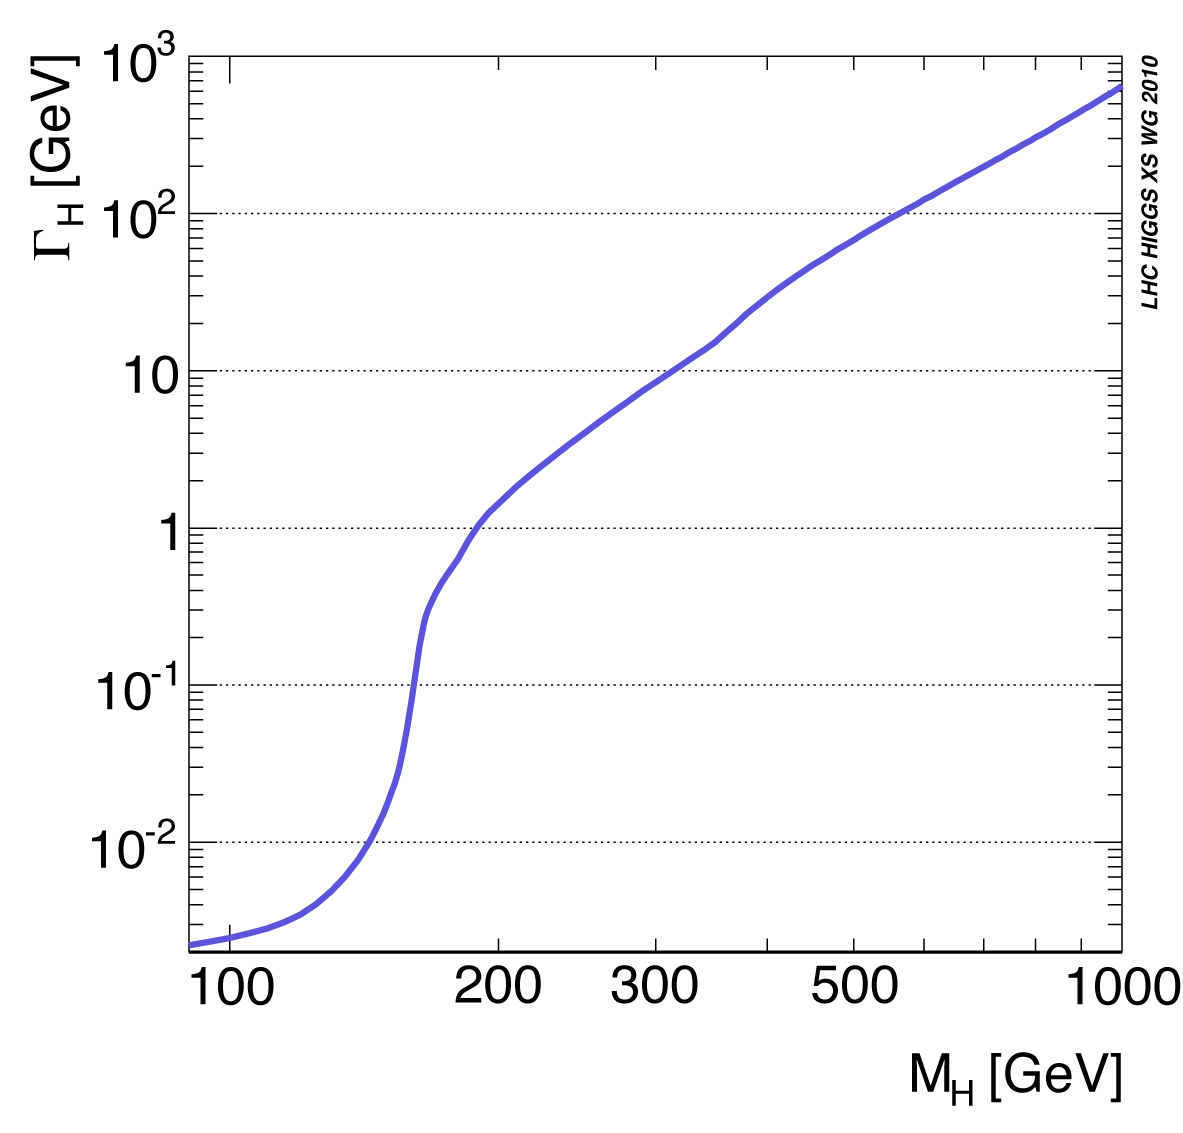
\includegraphics[width=0.42\textwidth]{figs/u0g5o.png}
    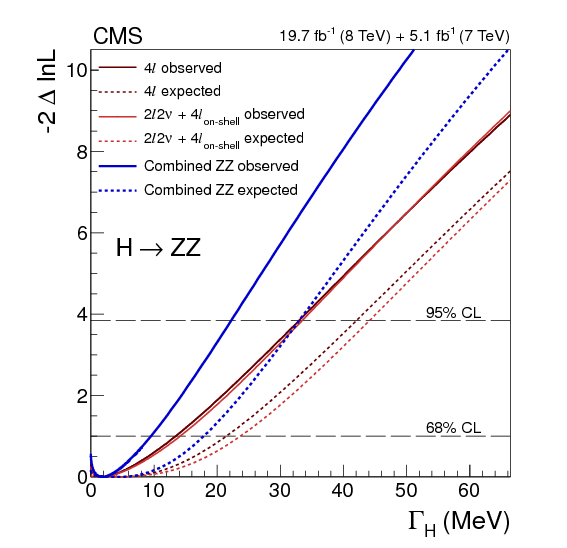
\includegraphics[width=0.42\textwidth]{figs/AllFitPaper_30_04_14_MeV.png}
    \caption{Higgs width as function of its mass [left] (from~\cite{Dittmaier:2011ti, Dittmaier:2012vm, Heinemeyer:2013tqa, HIGGSXSWG}) and current limits from CMS measurement [right] (from~\cite{Khachatryan:2014iha}).}
    \label{fig:WidthHiggs}
  \end{center}
\end{figure}

%\begin{figure}[!Hhtbp]
%  \begin{center}
%    
\includegraphics[width=0.3\textwidth]{figs/CMSlogo.png}
%    \caption{}
%    \label{fig:}
%  \end{center}
%\end{figure}
%\begin{TOINCLUDE}Plot on ATLAS+CMS combination of the Higgs mass; Plot on signal strength for each decay channel; Individual plots on diphoton channel and golden channel\end{TOINCLUDE}


%\begin{TOINCLUDE}Plot of branching ratio as function of the mass for different scenarios (representations)\end{TOINCLUDE}



%Detector chapter
\chapter[The CMS experiment at LHC]{The CMS experiment at LHC}

The CMS experiment is one of the biggest particle physics experiments on the world. It is located at the ring of the LHC that is the main accelerator managed by CERN, the European Organization for Nuclear Research or Centre Europ\'{e}enne pour la Recherche Nucl\'{e}aire by its french name. This center constitutes the biggest center for research on particle physics all over the world. All along its 60 years of existence, from 1954, 21 member states have been joining it, but an overall of 113 countries participate in different ways on this center. 

On the present chapter we discuss in detail different aspects of the LHC accelerator and the CMS experiment. In particular we make some emphasis in the CMS sub-detectors related to jets, objects that play the main role on the search that is the main subject of the present work. We also discuss the present state of both machines, their achievements and the challenges that were overcome. Finally, also the expectations and goals for the upcoming run II are mentioned.  

\section{The Large Hadron Collider}
\label{sec:LHC}

The Large Hadron Collider, or LHC~\cite{Bruning:782076}, is a machine that accelerates and collides protons and lead. This machine is the biggest particle collider nowadays with a circumference of 27 km. It also achieves the highest energy by a collider up to present, planned to be 14 TeV at the center of mass of the collision. On the first run of the machine only 8 TeV were achieved, and next run is planned to start with 13 TeV. It's located in French-Swiss border near to Geneva. The tunnel for the machine was carved around 100 m under the ground, 45 m under the Jura mountains and 170 m under the L\'{e}man lake with an inclination of around 1.4\%, sloping down towards the lake . This machine has used as much as possible old LEP buildings and sites, that was an electron-positron collider built between 1984 and 1989. 

The protons and heavy ions accelerated by the machine collide in different points where dedicated experiments are located to detect and study the product from the collisions. The four main experiments located on the LHC ring are CMS~\cite{Bayatian:922757,Bayatian:942733}, ATLAS~\cite{ATLAS:1999}, LHCb~\cite{Alves:2008zz} and ALICE~\cite{Cortese:879894}. The first two are experiments of generic purpose where searches for new physics and also precision measurements are performed. LHCb is dedicated to the physics of the b-quark, and ALICE focuses on the study of the quark-gluon plasma produced from heavy ions collisions. Even if one of the principal objectives of the construction of the LHC was the search for the Higgs boson, generic searches on new physics have been conducted from the very beginning of the first data taking in 2009. Moreover, after the Higgs discovery in 2012 there is a growing effort on the searches for new physics and precision measurement of the properties of the Higgs.

The LHC is a complex machine composed of several parts. The two principal parts are the injector chain and the main ring. A diagram of the whole CERN complex can be seen in figure~\ref{fig:Complex}. The injector chain has different stages that pre-accelerate protons and heavy ions to be injected into the main ring of LHC. %In the main ring the protons and heavy ions are fully accelerated and collided in four different points over the ring.

\begin{figure}[!Hhtbp]
  \begin{center}
    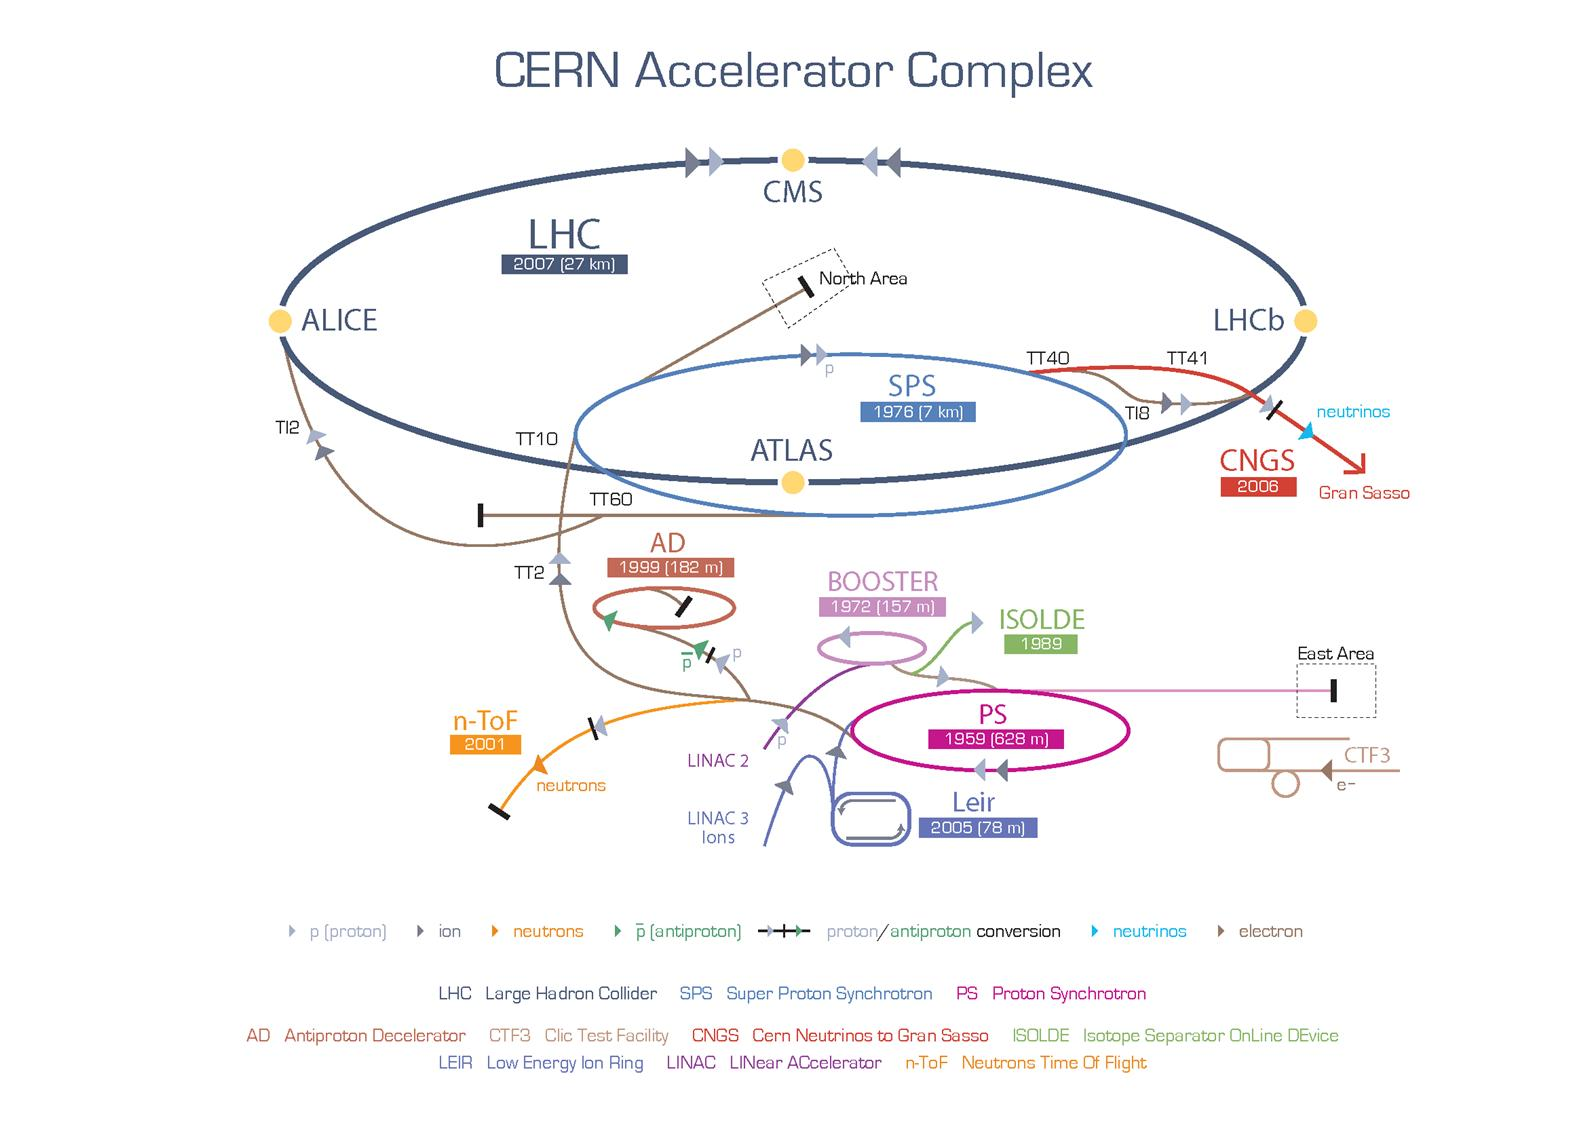
\includegraphics[trim=4.5cm 0cm 0cm 0cm, clip=true, width=1.15\textwidth]{figs/cern-lhc-4.jpg}
    \caption{Organization of CERN accelerator complex}
    \label{fig:Complex}
  \end{center}
\end{figure}

\subsection{Injector chain}
\label{sec:injector}

The injector chain begins with the proton source. Protons are extracted via ionization of Hydrogen gas in the Duoplasmatron Proton Ion Source. Such extraction is pulsed, what makes up the first bunch structure. The extracted protons are then accelerated up to 50 MeV in the linear accelerator, Linac2, that dates from 1978. After this first stage several steps are followed:
\begin{enumerate}
\item Linac2 injects proton bunches in the Proton Synchrotron Booster (PSB) where they are accelerated to 1.4 GeV. 
\item From PSB, the protons are delivered to the Proton Synchrotron (PS) where they reach an energy of 25 GeV. In the PS the bunches are also split from 6 initial bunches to 72 spaced by 25 ns.
\item Finally, the pre-acceleration chain is finished by the SPS, Super Proton Synchrotron. There the bunches are accelerated up to 450 GeV right before being inserted into the main LHC ring. 
\end{enumerate}

The whole pre-acceleration chain has been optimized to obtain the best possible performance on the final acceleration in the LHC main ring. All parameters are carefully controlled, for example the number of bunches, the separation between bunches, the separation between trains of bunches or the injection energy to each subsystem. It's also remarkable to notice the level of control achieved in the bunches manipulation, from old subsystems as the PS from 1959 or the newest, the SPS that dates from 1976. 

Some recent plans for future accelerator have been studied using the LHC main ring as injector for a bigger accelerator, for example the so called FCC (Future Circular Collider) at CERN. The FCC could be built perform proton-proton, electron-positron or electron-proton collisions, versions that are called respectively FCC-hh, FCC-ee and FCC-he. The FCC-hh is being designed to achieve 100 TeV of center of mass energy in a tunnel of 80-100 km of circumference. 

\subsection{Main ring}
\label{sec:ring}

The main ring is composed of two rings that accelerate the proton bunches in opposite directions, clock-wise and counter clock-wise. An schematic view of the design of the main ring can be seen in figure~\ref{fig:schematic}. The rings crosses in different points in order to collide the protons and they are divided in eight straight sections and eight arcs. In each octant bunches are controlled by dipole magnets. These complex magnets, in figure~\ref{fig:dipole}, need to produce a very strong magnetic field in order to be able to bend a 7 TeV beam of protons. This intense magnetic field, 8.33 T, in opposite directions, is produced by electrical currents that are only achievable by means of superconductivity. All the 1232 dipoles operate at a temperature of 1.9 K, under cooling by liquid helium. They also operate under ultra-high-vacuum. The beam lines with a pressure less than $10^{-9}$ mbar and the whole dipole system with $10^{-6}$ mbar, that serves also as insulating system from the surroundings. In addition, the LHC main ring has other magnets that focus and correct different characteristics of the beam: 520 quadrupoles, 2464 sextupoles, 1232 octupoles. 

\begin{figure}[!Hhtbp]
  \begin{center}
    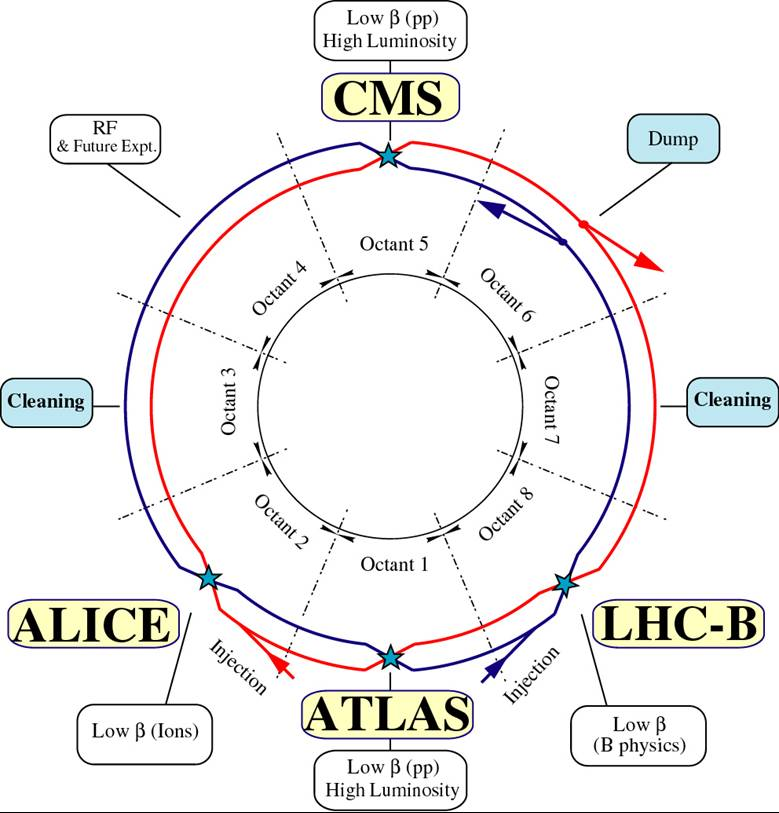
\includegraphics[width=0.8\textwidth]{figs/lhc-schematic.jpg}
    \caption{Schematic of the LHC main ring design.}
    \label{fig:schematic}
  \end{center}
\end{figure}

\begin{figure}[!Hhtbp]
  \begin{center}
    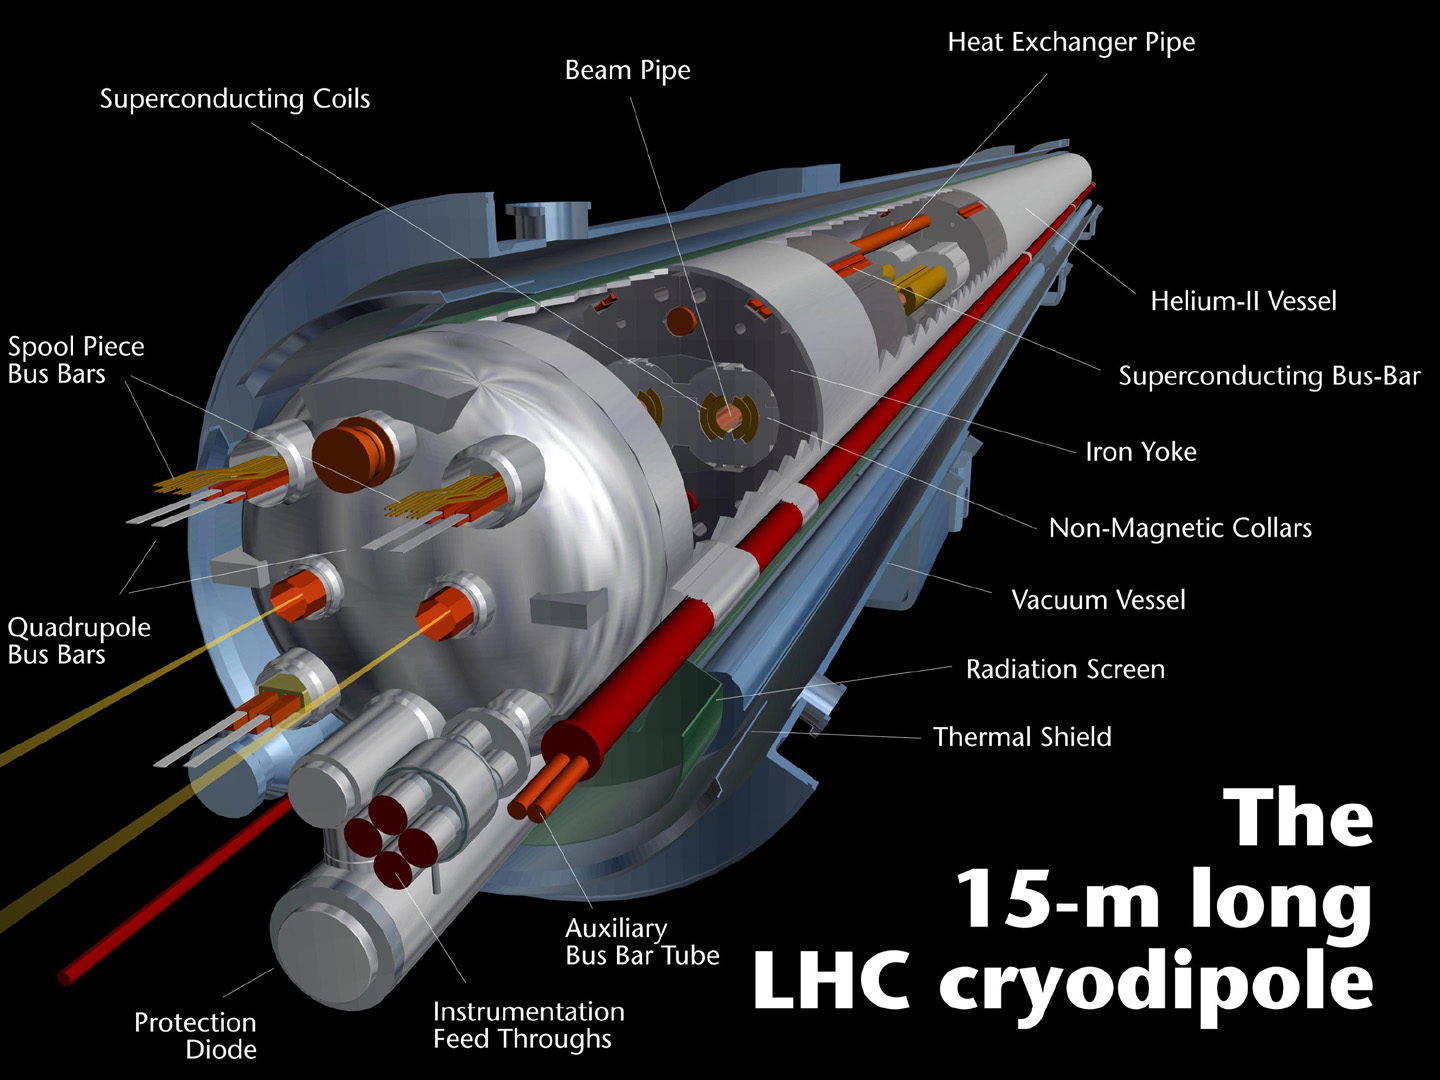
\includegraphics[width=0.45\textwidth]{figs/cryodipole.jpg}
    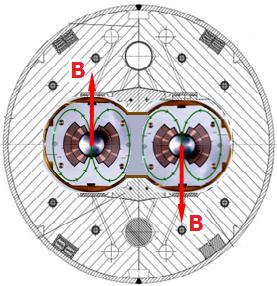
\includegraphics[width=0.45\textwidth]{figs/dipole_B.jpg}
    \caption{Design of LHC cryodipole and the magnetic field that bends the beam in the main ring.}
    \label{fig:dipole}
  \end{center}
\end{figure}

\subsubsection{Luminosity}
\label{sec:lumi}

In collider physics, such as the LHC, the figure of merit is the luminosity, given in equation~\ref{eq:lumiC}. The number of events per second is proportional to the luminosity, hence is the quantity to be maximized by the design and operation of the accelerator. The collider characteristics depend on the number of bunches in the ring $n_{b}$, the number of protons per bunch $N_{b}$, the revolution frequency $f_{rev}$, the relativistic gamma factor $\gamma$, the normalized rms transverse beam emittance $\epsilon_{n}$ and the beta function at the interaction point $\beta^{*}$. The denominator on~\ref{eq:lumiC} can also be rewritten in terms of the horizontal and vertical width of the bunches at the crossing, $\sigma^{*}_{x}$ and $\sigma^{*}_{y}$. In addition, there is the geometric reduction factor ($R$) that introduces a dependence on the crossing angle of the bunches at the interaction points. In table~\ref{tab:LHCparams} can be found the LHC beam parameters at injection and collision.  

\begin{equation}
  \label{eq:lumiC}
  L=\frac{n_{b}N_{b}^{2}f_{rev}\gamma}{4\pi\epsilon_{n}\beta^{*}}R=\frac{n_{b}N_{b}^{2}f_{rev}}{4\pi\sigma^{*}_{x}\sigma^{*}_{y}}R
\end{equation}

\begin{table}[htbH]
\label{tab:LHCparams}
\begin{center}
%\topcaption{LHC proton beam parameters.\label{tab:LHCparams}}
%\resizebox{\textwidth}{!}{
\begin{tabular}{|c|c c|}
\hline 
Parameter/units & Injection & Collision \\
\hline
Energy [GeV]& 450 & 7000 \\ 
Luminosity [$\text{cm}^{-2}\text{s}^{-1}$] & & $10^{34}$ \\
$k_{b}$ Number of bunches & \multicolumn{2}{c|}{2808} \\
Bunch spacing [ns] & \multicolumn{2}{c|}{24.95} \\
$N_{b}$ intensity per bunch [protons/bunch] & \multicolumn{2}{c|}{$1.15\times 10^{11}$} \\
Beam current [A] & \multicolumn{2}{c|}{0.58} \\
$\epsilon_{n}$ normalized rms transverse beam emittance [$\mu$m] & 3.5 & 3.75 \\ 
$f_{rev}$ revolution frequency [kHz] & \multicolumn{2}{c|}{11.25} \\
\hline
\end{tabular}
%}
\end{center}
\end{table}

At the crossing points, the number of events coming from collisions and produced via a specific process, is directly proportional to the luminosity provided by the collider, as in equation~\ref{eq:lumiC}.

\begin{equation}
  \label{eq:lumiN}
  N_{events}=L\sigma_{process}
\end{equation} where $\sigma_{process}$ is the cross section of the process. 

The total cross section of a proton-proton collision from the crossing of two bunches at 14 TeV is 100-110 mb~\cite{Augier:1993ta}, from three different scattering processes: elastic, diffractive and inelastic. In the elastic scattering the protons only exchange momenta but their structure remain unchanged, that is the case for the majority of collisions. In diffractive scattering momenta is exchanged and also new particles are produced in addition to the two final protons. Finally, in inelastic scattering, the constituents of the protons, the partons, interchange a big amount of momentum and produce a large quantity of particles. The inelastic processes contribute less than diffraction to the total cross section. While inelastic collisions produce particles in the central rapidity (defined in~\ref{sec:Csys}) region, diffractive and elastic final products have a large rapidity. Only in the hard interactions, inelastic scattering, color is exchanged, being the reason to fill up the central rapidity region. 

From the crossing of two bunches not only one proton-proton interaction is expected. In average, 25 interactions are expected for each crossing. From them, only one is coming from an inelastic collision, that is the type of process of more interest for detectors as CMS or ATLAS. This fact puts an additional difficulty to the detectors in order to extract the hard interaction from all the elastic and diffractive collisions happening at same time. Such phenomena is known as Pile-Up, an illustration of a collision with high pile-up can be found on figure~\ref{fig:pileup} as seen by the CMS detector.

\begin{figure}[!Hhtbp]
  \begin{center}
    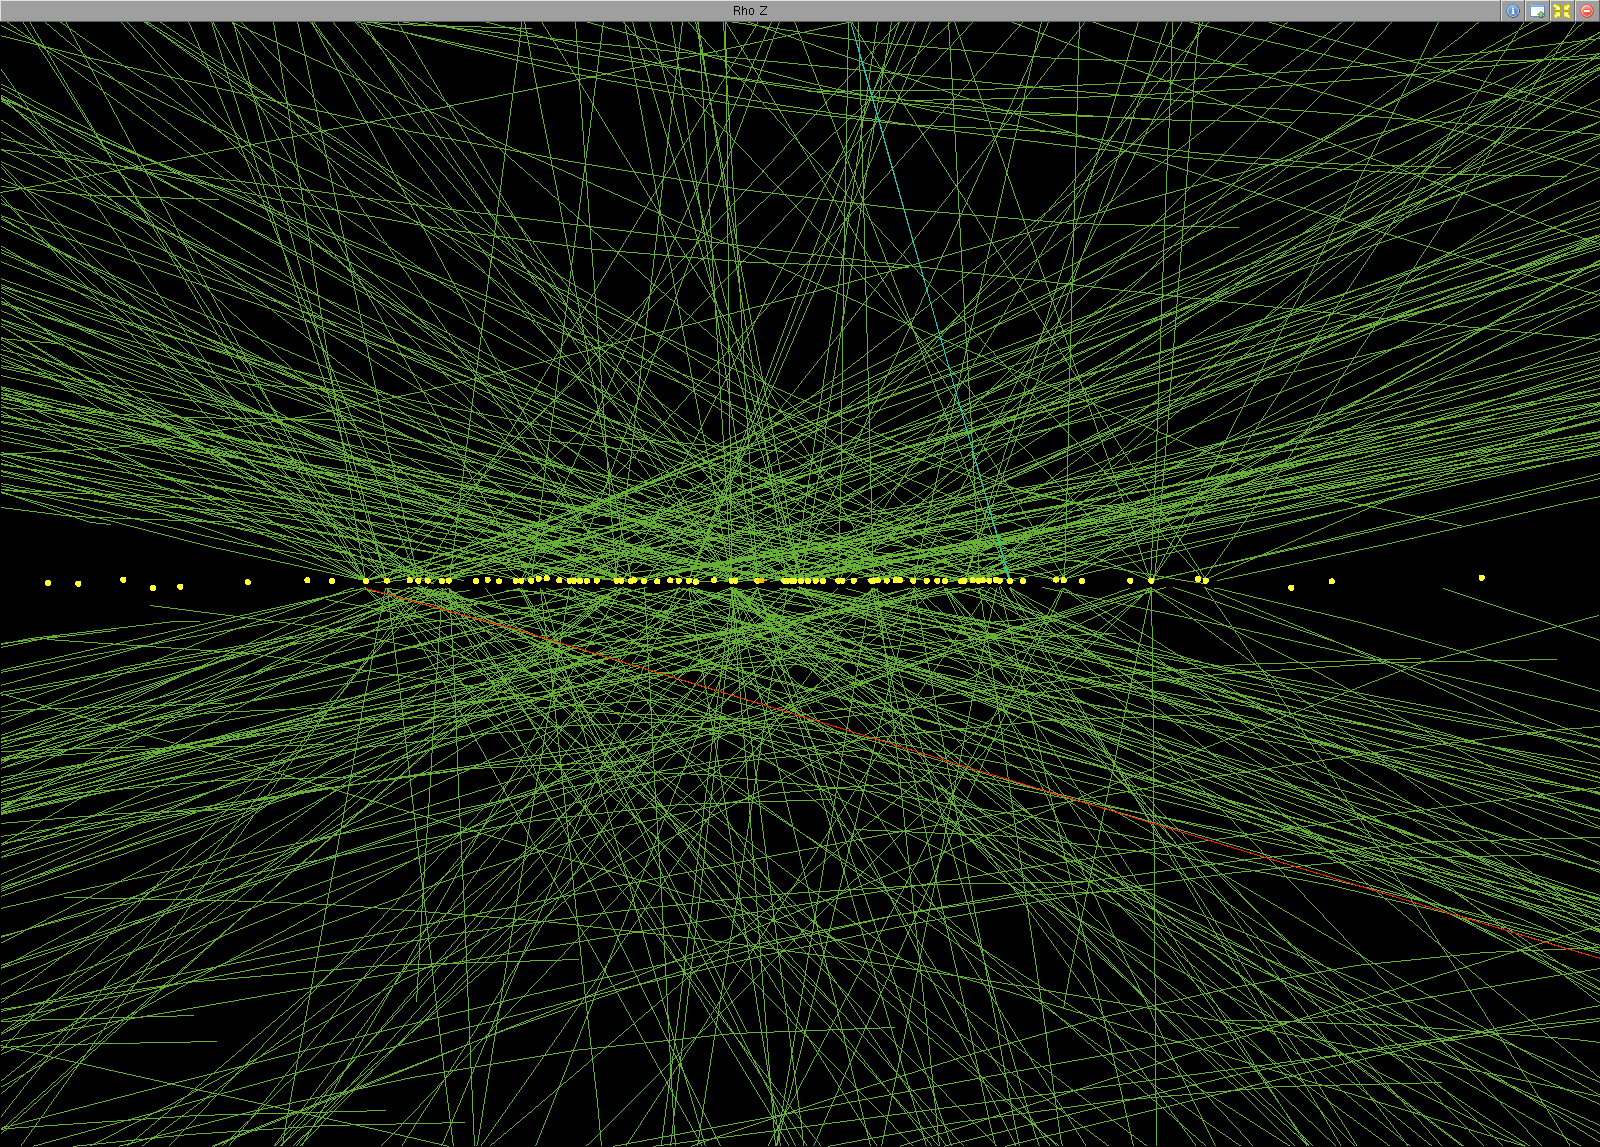
\includegraphics[width=0.7\textwidth]{figs/pileup.png}
    \caption{High pile-up event (78 interactions) seen by CMS detector. Event 35655522, from 198609 run, lumi 56, recorded on 2012. Image credit: Andre Holzner \copyright CERN}
    \label{fig:pileup}
  \end{center}
\end{figure}

\subsection{Run 1}
\label{sec:run1}

On February 10 of 2013 the first stable run of the LHC reached an end. This run, now called Run 1, started on November 20 of 2009. LHC was originally planned to start in 2008, but an incident on one of the electric connections of one of the magnets forced to stop on the 19th of September of the same year. From the restart in 2009, the energy was augmented from 450 GeV to 4 TeV per beam. The 23th of September 2009 the first collisions were detected by the experiments. One week after, the achieved center of mass energy was $\sqrt{s}=2.36$ TeV, already higher than Tevatron (0.98 TeV).

In 2010, from 30th March to 6th December 3.5 TeV per beam were reached delivering near 50 $\text{pb}^{-1}$. With the same energy, approximately 6 $\text{fb}^{-1}$ were delivered in 2011. 

In 2012, the center of mass energy reached one additional TeV, $\sqrt{s}=8$ TeV, and around 20 $\text{fb}^{-1}$ of integrated luminosity were delivered between April and December. On figure~\ref{fig:CMSlumi} can be seen the progress of the recorded luminosity by CMS for 2010-2012 period. The first six weeks of 2013 were devoted to proton-lead collisions.

After this very successful run, the LHC has been stopped for more than a year for repair and maintenance of different systems in the experiments and in the LHC itself to achieve higher energies. After this period, known as Long Shutdown  or LS1, the LHC is planned to restart a new run on the early spring of 2015.

\begin{figure}[!Hhtbp]
  \begin{center}
    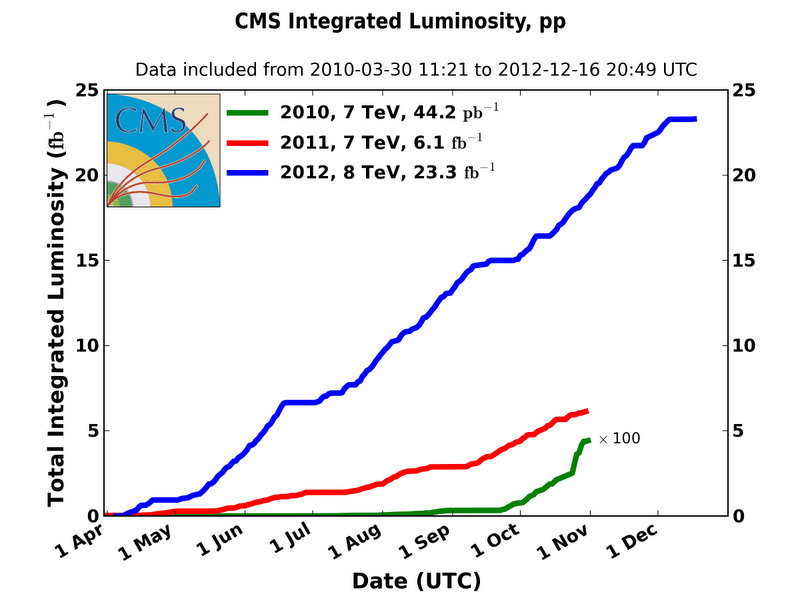
\includegraphics[width=0.7\textwidth]{figs/cms-int-10to12.jpg}
    \caption{CMS integrated luminosity for proton-proton collisions delivered by LHC. \copyright CERN}
    \label{fig:CMSlumi}
  \end{center}
\end{figure}

\subsection{Other experiments at LHC}
\label{sec:expers}

On the main ring there are several experiments depending on the collisions delivered by the LHC main ring. The biggest are CMS~\cite{Bayatian:922757} and ATLAS~\cite{ATLAS:1999}, both of them generalist experiments designed to do precision measurements as well as new physics searches. Mainly recording proton-proton collisions, they have also recorded lead-lead and proton-lead collisions during the run 1. Both of them were designed for high instantaneous luminosity, $L = 10^{34}\text{cm}^{2}\text{s}^{-1}$.

In addition, there is two other experiments designed for specific purposes. The LHCb~\cite{Alves:2008zz} that focus on the study of the physics of the b-hadrons, specially related to the CP violation, and ALICE~\cite{Cortese:879894} built for the study of strongly interacting matter. The first of them record proton-proton collisions at an instantaneous luminosity of $10^{32}\text{cm}^{2}\text{s}^{-1}$ and the second record ion-ion collision with $L = 10^{27}\text{cm}^{2}\text{s}^{-1}$.

The CMS experiment is going to be described in detail in section~\ref{sec:CMS}. In the following sections we are going to present very briefly the other three experiments mentioned above. 

\subsubsection{ATLAS}
\label{sec:atlas}

The ATLAS experiment (A Toroidal LHC ApparatuS) is the biggest LHC experiment. It's located at point one, as displayed on figure~\ref{fig:schematic}, on the LHC main ring. It's a cylindrical detector similar to CMS, about 45 meter long, 25 meter high, and weights around 7000 tons. ATLAS main components are, from inside to outside, a tracking system, an electromagnetic calorimeter, a hadron calorimeter and muon chambers. In between these subsystems there is an internal solenoidal magnet and a set of external toroidal magnets. The detector design is presented on figure~\ref{fig:atlasdet}.

\begin{figure}[!Hhtbp]
  \begin{center}
    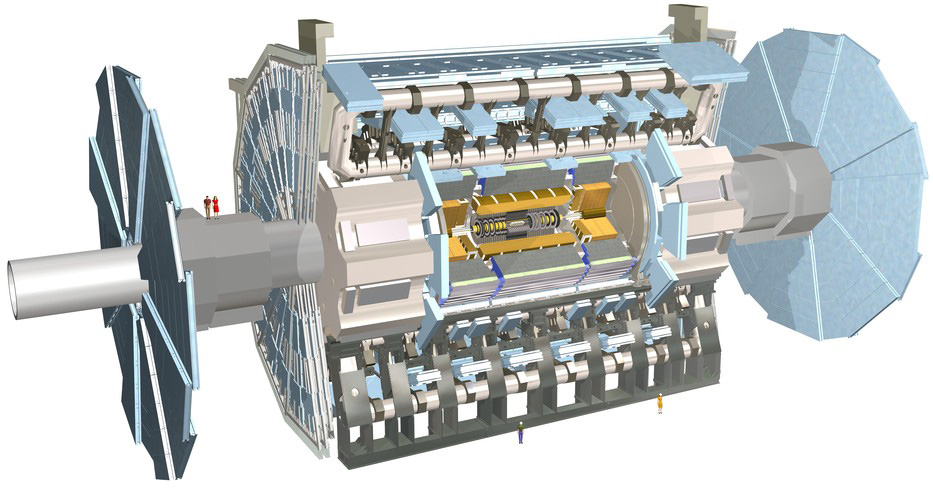
\includegraphics[width=0.7\textwidth]{figs/atlas_lg.jpg}
    \caption{ATLAS detector internal view. \copyright CERN}
    \label{fig:atlasdet}
  \end{center}
\end{figure}

On the human resources side, ATLAS experiment configures a collaboration of around 3000 persons, coming from 117 universities around the world, from 38 countries. Thirty percent of the collaboration are students.  

\subsubsection{LHCb}
\label{sec:lhcb}

LHCb detector, hosted at point 8 of the LHC main ring, has a different design than CMS and ATLAS. Smaller than these, its design mainly focus to be able to detect particles produced close to the beam direction. This is the reason why it is not cylindrically but conically shaped, in two detection arms~\ref{fig:lhcbdet}. It also has the same main parts, a tracking system with a very precise vertex locator, electromagnetic and hadron calorimeters, muon chambers and magnets. Its major specificity is a system that allows to identify different hadrons, the RICH detectors, a crucial feature for the study of strong interacting matter. It measures 21 m long, 10 m high and 13 m wide, and weights 4500 tons. A view of the detector can be found on figure~\ref{fig:lhcbdet}. The LHCb collaboration groups around 700 persons from 50 different universities over 15 countries. 

\begin{figure}[!Hhtbp]
  \begin{center}
    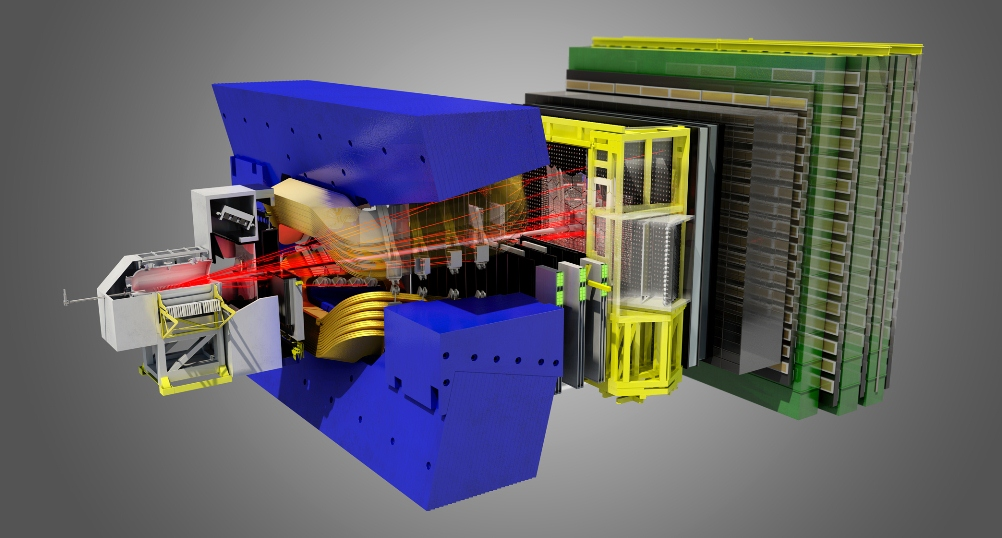
\includegraphics[width=0.8\textwidth]{figs/LHCbDetectorlight1.jpg}
    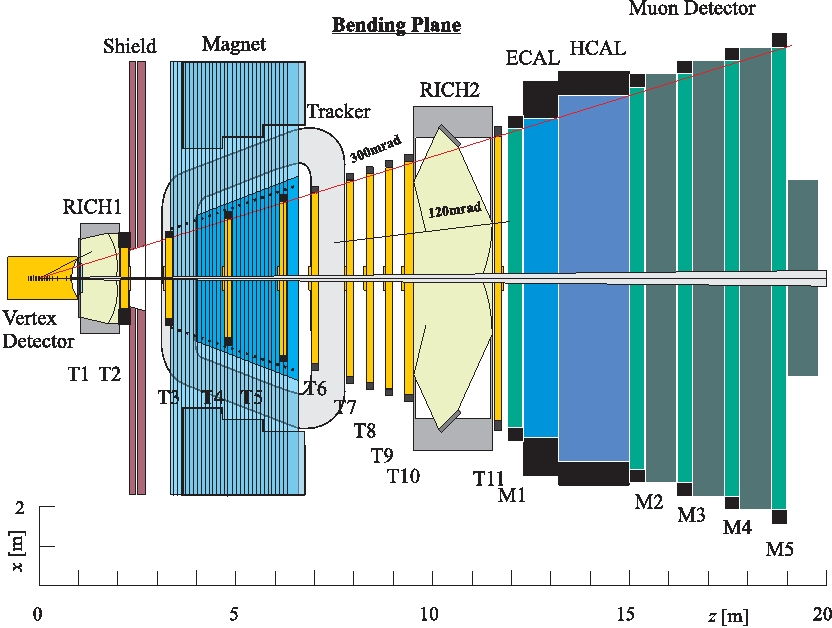
\includegraphics[width=0.8\textwidth]{figs/LHCb_UpView.jpg}
    \caption{LHCb detector internal view [top] and view from the top [bottom]. \copyright CERN}
    \label{fig:lhcbdet}
  \end{center}
\end{figure}

%\begin{figure}[!Hhtbp]
%  \begin{center}
%    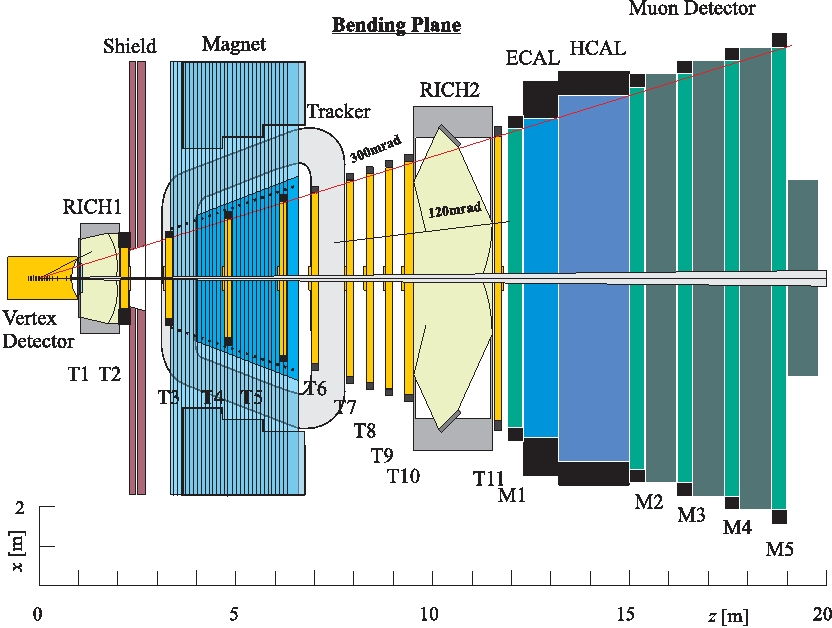
\includegraphics[width=0.7\textwidth]{figs/LHCb_UpView.jpg}
%    \caption{LHCb detector view from the top. \copyright CERN}
%    \label{fig:lhcbupview}
%  \end{center}
%\end{figure}

\subsubsection{ALICE}
\label{sec:alice}

The ALICE experiment (A Large Ion Collider Experiment) is located at point 2 of the LHC main ring, measures 16 m high, 16 m wide and 26 m long, and weights 10000 tons. Designed for heavy ion physics, it is able to detect an extremely high number of tracks per event. Its main subsystem is the Time Projection Chamber (TPC), a 90 $\text{m}^{3}$ gas chamber filled with a mixture of Ne, $\text{CO}_{2}$ and $\text{N}_{2}$ operated in a solenoid of 0.5 T. It allows to measure leptonic and hadronic charged particles in a momentum range from 0.5 to 10 GeV/c. The experiment structure can be seen on figure~\ref{fig:alicedet}. ALICE collaboration counts around 1500 people, from 154 physics institutes in 37 countries.

\begin{figure}[!Hhtbp]
  \begin{center}
    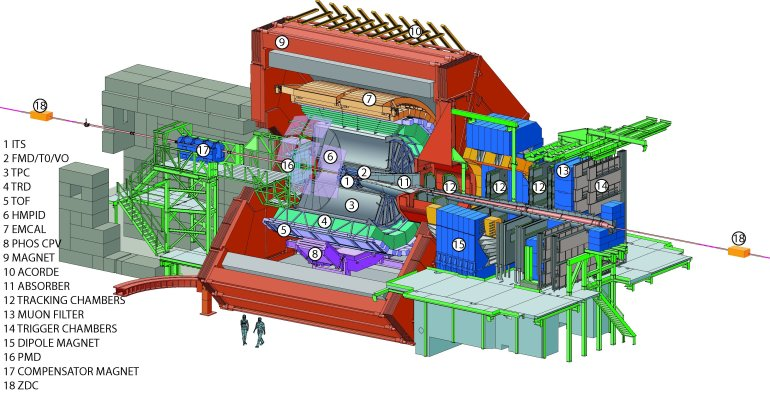
\includegraphics[width=0.8\textwidth]{figs/alice2.jpg}
    \caption{ALICE detector internal view. \copyright CERN}
    \label{fig:alicedet}
  \end{center}
\end{figure}

\section{The Compact Muon Solenoid (CMS) experiment}
\label{sec:CMS}

The CMS detector, hosted at point 5 of the LHC main ring (see figure~\ref{fig:schematic}), is the second biggest LHC experiment. Cylindrically shaped, measures 15 m of diameter and 28.7 m long, and weights 14000, making it the heaviest LHC experiment. Its subsystems are concentrically located from the collision point in the beam line. It's called compact because the whole calorimetry is inside the solenoid magnet, and muon solenoid because it has a very precise muon detection. Its main characteristic is the strong 3.8 T solenoid magnet. A representation of the detector can be found in figure~\ref{fig:cmsdet}. The CMS collaboration is formed by around 2600 scientists, of which 900 are students, from 181 institutes over 41 countries. 

\begin{figure}[!Hhtbp]
  \begin{center}
    \includegraphics[width=\textwidth]{figs/CMS_det.pdf}
    \caption{CMS detector internal view. \copyright CERN}
    \label{fig:cmsdet}
  \end{center}
\end{figure}

CMS has been designed to be able to do very precise identification of particles originated from the collisions and their properties. For the measurement of the momentum of the charged particles, CMS counts with a very strong magnet that allows to bend very energetic particles. In addition, the calorimeters allow to measure accurately the energy from hadrons, electrons and photons. At the most external layer, the muons chambers measuring muons properties, and in the innermost the tracking system that reconstructs the collision points and the charged particles tracks. In figure~\ref{fig:cmsslice} can be found a representation of the different subsystems of CMS and how particles are reconstructed from them.

\begin{figure}[!Hhtbp]
  \begin{center}
    \includegraphics[width=\textwidth]{figs/PictureforPoint5_oct04_allp.jpg}
    \caption{CMS sub-detectors and particle identification. \copyright CERN}
    \label{fig:cmsslice}
  \end{center}
\end{figure}

\subsection{Coordinate system}
\label{sec:Csys}

The origin of coordinates defined on the CMS detector is located on the nominal collision point, the ``interaction point''. From there, the z-axis is defined along the beam pipe line pointing towards the Jura mountains. The positive/negative z-axis directions define the positive/negative sides of the detector. The y-axis is defined towards the zenith and the x-axis towards the center of the LHC ring. Due to the inclination of the LHC plane, this coordinate system is slightly tilted with respect to the true vertical. A representation of the coordinate system definition can be found in figure~\ref{fig:cmscoor}. 

\begin{figure}[!Hhtbp]
  \begin{center}
    \includegraphics[width=\textwidth]{figs/CMS_coordinates.jpg}
    \caption{CMS coordinate system. \copyright CERN}
    \label{fig:cmscoor}
  \end{center}
\end{figure}

We can also define two angles: the $\phi$ angle in the x-y plane from the x-axis towards the positive y-axis, and the $\theta$ angle in the z-y plane from z-axis towards the positive y-axis. In experimental particle physics is preferred to work with relativistic invariant quantities, reason why instead of working with $\theta$ we define the pseudorapidity $\eta$, equation~\ref{eq:pseudorapidity}. 

\begin{equation}
  \label{eq:pseudorapidity}
  \eta = -\text{ln}\left( \text{tan}\left(\frac{\theta}{2}\right)\right)
\end{equation} 

One can define another relativistic invariant quantity, the rapidity $y$ as from equation~\ref{eq:rapidity}. With $\bm{p}$ being the momentum vector and $E$ the energy of a given particle, $p_{L}$ denotes its longitudinal component, that in our case is the same z-component. 

\begin{equation}
  \label{eq:rapidity}
  y=\frac{1}{2}\text{ln}\left(\frac{E+p_{L}}{E-p_{L}}\right)
\end{equation}On the limit that the mass of the particle is very small compared to its momentum, one can replace approximate the particle energy by the momentum magnitude, giving rise to the definition of the pseudorapidity in terms of the momentum of the particle $\eta = \frac{1}{2}\text{ln}\left(\frac{\bm{p}+p_{L}}{\bm{p}-p_{L}}\right)$

We define also the radial coordinate over the x-y plane, plane that is called the transverse plane being orthogonal to the longitudinal direction, the z-axis. In such plane are also defined the transverse quantities of particles, as the transverse momentum $p_{T}$. Finally, for any two objects an angular distance can be defined in the $\eta-\phi$ plane, as in equation~\ref{eq:deltaR}.

\begin{equation}
  \label{eq:deltaR}
  \Delta R=\sqrt{(\Delta\eta)^{2}+(\Delta\phi)^{2}}
\end{equation}

\subsection{Magnet}
\label{sec:magnet}

In order to measure the momentum of the charged particles going inside the detector is crucial to apply the correct magnet field, sufficiently strong to bend very energetic particles. The momentum of a charged particle inside an uniform magnetic field can be written as

\begin{equation}
  \label{eq:momB}
  p=\gamma m v=qBr
\end{equation} where $B$ is the magnitude of the magnetic field, $\gamma$ the usual relativistic factor, $m$ the mass of the particle, $v$ its rapidity, $q$ its charge and $r$ the bending radius. The sagitta of the arc is

\begin{equation}
  \label{eq:sagitta}
  s=\frac{L^{2}}{8r}=\frac{qBL^{2}}{8p}
\end{equation} with $L$ the trajectory length that the particle moved inside the magnetic field. Inside a solenoid $L$ is equal to the radius of it. 

From relation~\ref{eq:sagitta} it is possible to deduce that the resolution on the momentum of the particle has an inverse dependence with the magnetic field and the radius of the solenoid, as shown in equation~\ref{eq:presolution}. From there, for a better resolution it is needed to increase the magnetic field and the radius of the solenoid. 

\begin{equation}
  \label{eq:presolution}
  \frac{dp}{p}\propto \frac{p}{BL^{2}}
\end{equation}

The design of CMS magnet target both features, it utilizes a large solenoid of 6 m of diameter and 13 m long. It's made of 4 layers of windings of NbTi cable that is cooled to 4.45 K in order to achieve the superconducting state. This magnet is able to produce an uniform magnetic field inside of it of 3.8 T. Outside the magnet 5 wheels and 3 disks of iron are placed in order to return the flux of the magnetic field, inducing just a 2 T radial magnetic field outside the solenoid. This iron yoke is the main contribution to the detector weight, 10000 tons. The muon chambers are located in between the iron yoke.

\subsection{Tracker system}
\label{sec:tracker}

The tracker system has been designed to specifically address the reconstruction of high pt leptons, with particular interest in the isolation of electrons and, as a consequence, to isolate photons. Also the tracker fulfill granularity requirements to reconstruct secondary vertexes to tag and reconstruct B-hadrons. The tracker system is able to reconstruct tracks of particles with at least 2 GeV of $p_{T}$ with $|\eta|<2.5$. Charged hadrons are reconstructed with an efficiency of at least 85\% for $p_{T}=1$ GeV and up to 95\% for $p_{T}$ above 10 GeV. Another important point that was taken into account is the fact that the tracker is the part of CMS most exposed to radiation as it is the closest subsystem to the interaction point. The tracker system was built highly resistant to radiation damage and is expected to last for around 10 years. The pixel detector only lasts 2 years and was replaces during LS1. 

The tracker has been built with three different technologies: Pixels, Silicon Strips and Micro Strip Gas Chambers (MSGCs). They are arranged concentrically in cylindrical volumes being the pixel detector the innermost and the MSGCs the outermost. The CMS tracker extends to a radius of 155 cm and a around 270 cm on each $z$ direction. The pixel system is in the region with a radius below $\approx$ 20 cm, the silicon detector between $\approx 20$ cm and $\approx 60$ cm, and the MSGCs between $\approx 70$ cm and $\approx 120$ cm. The three subsystems are fast enough to work at 25 ns scale.

The pixel system is formed by three barrel layers and two end caps disks covering radii from 6 cm to 15 cm. It has an approximate active surface of one square meter with approximately $40\times10^{6}$ channels with a cell size of 150 $\mu$m by 150 $\mu$m. This pixel system allows to obtain three highly precise points that are mainly used for reconstructing vertexes.

The Silicon Strip system is formed by a 5-layer barrel (TIB for Tracker Inner Barrel) and 10 disks (TID for Tracker Inner Disks) in each end cap. The strips length is 12.5 cm with a pitch from 61 $\mu$m to 122 $\mu$m for single-sided strips and for 81 $\mu$m to 244 $\mu$m for double-sided. It's able to achieve a hit resolution of about 15 $\mu$m. 

The MSGCs systems is composed of 6 layers in the barrel (TOB for Tracker Outer Barrel) and 11 disks in each end cap (TEC for Tracker EndCap, with a $\pm$ sign depending on the $z$ direction). Here the strips are 10 cm length for the inner layers and 25 cm for outer layers with a pitch from 200 $\mu$m to 400 $\mu$m, which gives a hit resolution of 35 $\mu$m and 100 $\mu$m respectively. The MSGCs and Silicon systems have an overall active area of around 300 $\text{m}^{2}$ with 12 $\times10^{6}$ channels organized in more than ten thousand independent modules.

In figure~\ref{fig:cmstracker} can be seen the disposition of all the tracker subsystems. From the design of the tracker system the best resolution on the $p_{T}$ measurement is achieved in the $|\eta|<1.6$ region, this due to the presence of more layers of detector in the different subsystems, as shown in figure~\ref{fig:trackerres}. 

\begin{figure}[!Hhtbp]
  \begin{center}
    \includegraphics[width=0.9\textwidth]{figs/fig_cmstracker.png}
    \caption{CMS tracker system configuration. \copyright CERN}
    \label{fig:cmstracker}
  \end{center}
\end{figure}

\begin{figure}[!Hhtbp]
  \begin{center}
    \includegraphics[width=0.9\textwidth]{figs/tracker_resolution.png}
    \caption{Tracker resolution with $\eta$. \copyright CERN}
    \label{fig:trackerres}
  \end{center}
\end{figure}

\begin{TOINCLUDE}Two plots: on pixel resolution and efficiency on finding hits\end{TOINCLUDE}

\subsection{Electromagnetic calorimeter}
\label{sec:ecal}

The CMS ECAL (Electromagnetic CALorimeter) is the detector subsystem designed to stop photons and electrons to measure their energy. It's an hermetic cylindrical calorimeter made of 61200 crystals in the barrel ($|\eta|<1.479$) and 7324 in each end cap ($1.48<|\eta|<3$). The crystals material is lead-tungstate that is transparent, very dense (8.28 g/$\text{cm}^{3}$), has a small Moliere radius (2.2 cm) and a short radiation depth ($X_{0}=0.89$ cm). This material has been chosen for the characteristics already described, but also because is very fast emitting the scintillation light (in 25 ns), it has a very good energy resolution and resistance to radiation. The crystals are distributed in 36 super-modules, 1700 crystals each, in the barrel (EB for ECAL Barrel) and in four 'Dee's, of 3662 crystals each, in the end caps (EE for ECAL End cap). In the EB the scintillation light is collected by Avalanche Photo-Diodes, or APD, and by Vacuum Photo-Triodes, or VPT, in the EE. A preshower system is installed in face of each end cap to allow a better discrimination between photons and $\pi^{0}$'s. A representation of the CMS ECAL can be found on figure~\ref{fig:ecal}.

\begin{figure}[!Hhtbp]
  \begin{center}
    \includegraphics[width=0.9\textwidth]{figs/ECAL.png}
    \caption{CMS ECAL representation. \copyright CERN}
    \label{fig:ecal}
  \end{center}
\end{figure}

\begin{TOINCLUDE}Plot on cristal response, dielectron reconstruction on the ECAL, ratio of E/p for reconstructed electrons E from the ECAL and p from the tracker\end{TOINCLUDE}

\subsection{Hadronic Calorimeter}
\label{sec:hcal}

The CMS HCAL, for Hadronic CALorimeter, is the subdetector designed to measure the energy of hadrons produced in the collisions, mainly the neutral hadrons because the charged hadrons are already traced by the tracker. It's also designed to measure the missing energy coming from particles not being detected by any of the subsystems, as neutrinos. It's an hermetic set of subsystems covering up to $|\eta|<5.2$:
\begin{itemize}
\item Hadron Barrel Calorimeter (HB): Covering $|\eta|<1.4$ is located between the ECAL barrel and the magnet. 
\item Hadron Endcap Calorimeter (HE): Extends the coverage of the barrel on the region $1.4<|\eta|<3$.
\item Hadron Outer Calorimeter (HO): Located outside the magnet, uses it as an additional absorber.
\item Hadron Forward Calorimeter (HF): Completes the coverage of the system from $|\eta|=3$ up to $|\eta|=5.2$.
\end{itemize}

The CMS HCAL layout is shown in figure~\ref{fig:hcal}. The system is made of two parts, an absorber to develop the hadronic showers and a scintillator to measure the particles energy. The length scale of hadronic calorimetry is designated as the interaction length corresponding to the mean free path of an hadron in a material. The HB absorber is made of 40 mm thick steel plate, eight layers of brass plates of 50.5 mm thick, six brass plates of 56.5 mm thick and a steel plate of 75 mm thick. The HE uses the same absorber but with thicker plates, of 79 mm. Between the absorber plates a plastic scintillator, Kuraray SCSN81, of 3.7 mm thick is placed. In the region with $|\eta|<1.6$ the achieved granularity is $\Delta\eta\times\Delta\phi=0.087\times 0.087$ and $\Delta\eta\times\Delta\phi=0.17\times 0.17$ in the region with $|\eta|>1.6$. This design gives a total of 70000 tiles used. The produced light in the HB is collected by optical fibers and transferred to the Hybrid Photo Diodes (HPDs). This diodes were chosen thanks to their small sensitivity to the magnetic field, an important feature due to the proximity of the HCAL to the magnet.

\begin{figure}[!Hhtbp]
  \begin{center}
    \includegraphics[width=0.9\textwidth]{figs/HCAL.png}
    \caption{CMS HCAL representation. \copyright CERN}
    \label{fig:hcal}
  \end{center}
\end{figure}

The HF design is very different from the rest of the HCAL subsystems. The most important challenge for the HF is the high resistance to radiation, while in the central rapidity region 100 GeV are deposited in average in the forward region is 760 GeV. For this reason it was chosen a Cherenkov detector made of quartz fibers with a steel absorber. The light produced in the HF is collected by photo multipliers. 

\subsection{Muon chambers}
\label{sec:muons}

The muon system of CMS is located at the most exterior layer of the detector  due to the penetration power of this particle. Muons are not stopped by the calorimeters and, with neutrinos, they are able to escape the detector. The muon chambers are placed in a cylinder around the HO and in disks on the end caps. Three main characteristics have been fulfilled from the design: efficient muon identification, precision measurement of muon charge and momentum and fast measurement to provide trigger capabilities. The moun chambers are made of three different subsystems:
\begin{itemize}
\item Drift Tubes Chambers (DT): Located in the region with $|\eta|<1.2$ and disposed in four layers. They consist of individual drift tubes of 50 $\mu$m of diameter anode wire with two electrode plates creating a drift electric field. The wall of the cell act as cathode. The cells are filled with a gas mixture, 85\% Argon and 15\% $\text{CO}_{2}$. The tubes are organized in plaques that are also organized in SuperLayers (SL) each one made of 4 plaques. The barrel is made of 250 DT's disposed in four cylinders separated by iron yokes. 
\item Cathode Strip Chambers (CSC): Installed in the end caps, provide a coverage up to $|\eta|=2.4$ from $|\eta|=0.9$. These chambers are multi-wire proportional chambers made of six planes of anode wires with 7 cathode planes. Four CSC stations are placed in each end cap. The wires are oriented in azimuthal direction while the cathode planes are radially oriented, allowing a complete measurement of the position of the particle. This system is able to measure with a precision between the 75 $\mu$m and 150$\mu$m.
\item Resistive Plate Chambers (RPC): This subsystem is made of gaseous parallel plate detectors. This detector is specially useful for triggering as it is very fast and have a good position resolution. There are 480 RPC distributed in 6 layers in the barrel with the DT and in 3 layers in the end caps with the CSC, and covers the region with $|\eta|<1.6$. 
\end{itemize}

On figure~\ref{fig:cmsmuon} can be found a representation of the muon system with the different components. The DT and CSC system cover $|\eta|<2.4$ without any gap. 

\begin{figure}[!Hhtbp]
  \begin{center}
    \includegraphics[width=0.9\textwidth]{figs/MuonDetector.png}
    \caption{CMS muon chambers representation. \copyright CERN}
    \label{fig:cmsmuon}
  \end{center}
\end{figure}

\begin{TOINCLUDE}Plot of RPC efficiency during Run1 and L1 RPC efficiency as function of probe PT\end{TOINCLUDE}

\subsection{Trigger}
\label{sec:trigger}

LHC has been designed to provide experiments with proton-proton collisions every 25 ns, meaning a frequency of 40 MHz. Each recorded event by CMS has a nominal size between 0.5 and 1 MB, what means a data flux of around $10^{9}\; \text{MB/s}= 1\text{PB/s}$ that is extremely big for transfer and for storing. Therefore, an on-line selection of events has to be done. The trigger system of CMS does this task in two fold, a level 1 (L1) and a high level trigger (HLT). The L1 is hardware based and the HLT is software based. 

From the searches conducted at CMS, the interesting events produced on proton-proton collisions for new physics searches are very rare. The enormous majority of events coming from proton-proton collisions correspond to well understood phenomena, while new physics events are 'exotic' with regards to the most common type of events. Then is interesting to keep only a part of the events, what actually easies the analysis afterward done over the data. 

The CMS trigger system is designed to keep only 100 kHz tops by the L1 and 300 Hz by the HLT. L1 is reducing the data flux by 2 orders of magnitude and the HLT another 3 orders of magnitude.

\subsubsection{Level 1 trigger}
\label{sec:L1}

The L1 is designed to trigger over coarse data coming from the calorimeters and muon chambers, holding data in pipe-lined memories in the front-end electronics. Therefore, relies on very fast reconstruction of objects coming from this subsystems: muons, electrons, photons, jets and missing energy. This reconstruction differs from the final reconstruction of the objects, for example a jet for the L1 consists on successive energy deposits in the ECAL and HCAL, while the off-line reconstruction take into account also the tracker information. 

The L1 starts from regional data coming from the subsystems which is afterward combined in order to build ranked trigger objects in localized regions of the detector. Global Muon and Calorimeter triggers sort the objects and send the best ranked to the Global Trigger (GT). Before the GT no events are rejected, is only with the GT that the selection is applied. The GT combines the information and can apply topological requirements and take a decision on keeping or disregarding the event. On figure~\ref{fig:l1} can be found the work-flow of the L1. 

\begin{figure}[!Hhtbp]
  \begin{center}
    \includegraphics[width=0.9\textwidth]{figs/img_l1.png}
    \caption{L1 architecture. \copyright CERN}
    \label{fig:l1}
  \end{center}
\end{figure}

The L1 cards are distributed between the detector and an adjoin cavern at 90 m distance from the detector. The latency time L1 disposes between the collision and the taking of the decision is about 3.2 $\mu$s. Therefore, the front-end memory in the cards should be able to keep in memory up to 128 bunch crossings. 

\subsubsection{High Level Trigger}
\label{sec:HLT}

The HLT take as input the events accepted by the L1 and process them using farms of commercial processors. The HLT does additional operations on the selected events making it much slower than L1 processing. In particular, the HLT takes also into account the tracker information. Consequently, this system is able to take into consideration the whole information of the detector. However, the reconstruction of objects done by the HLT differs slightly from the final off-line reconstruction. The decision taking process takes around 40 ms, $10^{4}$ times more than for L1. 

The events selected by HLT are finally stocked on disks under several paths depending on the selection performed. There is a constant development of HLT paths focusing on different analysis requirements in order to obtain the best possible selection efficiency for specific signal types. 

\section{Object reconstruction}

\subsection{Track and vertex reconstruction}

\begin{TOINCLUDE}Plots: Tracker efficiency reconstruction for muons and single pions as function of pt and eta\end{TOINCLUDE}

\subsubsection{Vertex reconstruction}

\begin{TOINCLUDE}Two plots: Primary vertex resolutions and Primary vertex efficiency\end{TOINCLUDE}

\subsection{Particle Flow (PF) algorithm}

\subsubsection{Calorimeter clustering}

\subsubsection{Subdetectors link}

\begin{TOINCLUDE}Two plots: Link of tracks to ECAL and to HCAL\end{TOINCLUDE}

\subsubsection{Particle reconstruction}

\subsection{Electron reconstruction}

\begin{TOINCLUDE}Plot of electron efficiency. Table with electron ID requirements\end{TOINCLUDE}

\subsection{Muon reconstruction}

\begin{TOINCLUDE}Plots: PF muon efficiency selection, dimuon mass spectra\end{TOINCLUDE}

\subsection{Jet reconstruction}

\subsubsection{Clustering algorithms}

\paragraph{SISCone}

\paragraph{kT}

\paragraph{Cambridge-Aachen}

\paragraph{Anti-kT}

\paragraph{Infrared and collinear safety}

\paragraph{Jet area}

\begin{TOINCLUDE}Plots: Jet in y-phi-pT space for each algorithm\end{TOINCLUDE}

\subsubsection{Jet energy corrections}

\begin{TOINCLUDE}Plot of JEC uncertainity as pT function and eta\end{TOINCLUDE}

\subsubsection{b-jets identification}

\paragraph{Identification algorithms and working points}

\begin{TOINCLUDE}Plots: CSV discriminator, Nb of secondary vertices, Efficiency of b-tagging for CSVM as function of PT and eta\end{TOINCLUDE}

\subsection{Photon reconstruction}

\begin{TOINCLUDE}Plot of photon identification efficiency\end{TOINCLUDE}

\subsection{Missing energy reconstruction}


%Add RUNII perspectives? Add section on dataset structure used by CMS?

%  LocalWords:  emittance ApparatuS


%VLQ chapter
\chapter[VLQ models]{Vector Like Quarks: Generic model}
\label{chap:VLQ}

From chapter~\ref{chap:SM} we have seen how there are some parts in the SM that does not work very well. From such internal issues some further models/theories have been developed. All this theories are commonly grouped under the term Beyond Standard Model or simply BSM. One of the most famous BSM theory is supersymmetry (SUSY). This theory postulates a symmetry that does not distinguish between fermions and bosons. This idea have given birth to a plethora of model realizations and physics predictions. So far, nothing of the new consequences of this theory have been confirmed but the experiments have an enormous investment on their search. But not only SUSY have seen the day light, there is on the market an astonishing amount of BSM theories addressing different issues of the SM. Extra dimensions, fourth families, composite Higgs are a few of them.

In this chapter we will describe a bunch of models that introduce additional heavy quarks, heavier than the top, in order to solve the hierarchy problem, described on section~\ref{sec:hier}. 

\section{Motivation}
\label{sec:motiv}

Why to introduce extra quarks.

Plausible solution of hierarchy problem.

Reference to models with extra quarks. (?)

\section{Generic Formulation}
\label{sec:form}

Formalism: Generic Langranian. Description of mixings with SM quarks.

\begin{table}[htbH]
\label{tab:VLQRepre}
\begin{center}
\begin{tabular}{|c|c|c|}
%\hline 
xxxxxxx & xxxxxxx & xxxxxxx
%\hline
\end{tabular}
\caption{Possible VLQ representations and correponding $SU(2)_{L}\times U(1)$ charges.}
\end{center}
\end{table}
%\begin{TOINCLUDE}Table with different possible representations and assigned charges\end{TOINCLUDE}

\subsection{Production modes}
\label{sec:prod}

Description of pair and single production. Parallel to production modes of top. Comparison between cross sections for pair and single production.

\begin{figure}[!Hhtbp]
  \begin{center}
    \includegraphics[width=0.3\textwidth]{figs/CMSlogo.png}
    \caption{Feynman diagrams of $T$ production in pairs [left] and single [right]}
    \label{fig:ProdDiag}
  \end{center}
\end{figure}

\begin{figure}[!Hhtbp]
  \begin{center}
    \includegraphics[width=0.3\textwidth]{figs/CMSlogo.png}
    \caption{$T$ production cross section for pair and single case as function of $T$ mass for different center of mass energy in proton-proton collisions.}
    \label{fig:TProdXS}
  \end{center}
\end{figure}
%\begin{TOINCLUDE}Plot of production cross section at LHC for different energies as function of the mass. Feynman diagrams of the production processes.\end{TOINCLUDE}

\subsection{Decay modes}
\label{sec:decay}

Description of possible decay channels of $T$. Relative importance of decay channels depending on the mass. 

\begin{figure}[!Hhtbp]
  \begin{center}
    \includegraphics[width=0.3\textwidth]{figs/CMSlogo.png}
    \caption{$T$ branching ratios as function of its mass.}
    \label{fig:TBRs}
  \end{center}
\end{figure}
%\begin{TOINCLUDE}Plot of branching ratio as function of the mass for different scenarios (representations)\end{TOINCLUDE}

\section{Fesability study for a search of a $T$ at LHC at 8 TeV}
\label{sec:pheno}

Discussion on selection of full hadronic channel.

\subsection{Stragey for the full hadronic final state}
\label{sec:Pstra}

General discussion of strategy used for selection. 

\begin{table}[htbH]
\label{tab:BKGS}
\begin{center}
\begin{tabular}{|c|c|c|}
%\hline 
xxxxxxx & xxxxxxx & xxxxxxx
%\hline
\end{tabular}
\caption{Cross sections and expected number of events for background processes and signal.}
\end{center}
\end{table}

\begin{figure}[!Hhtbp]
  \begin{center}
    \includegraphics[width=0.3\textwidth]{figs/CMSlogo.png}
    \caption{Forward jet produced in association with T.}
    \label{fig:ForwJ}
  \end{center}
\end{figure}
%\begin{TOINCLUDE}Table with cross sections and expected events for each background process and signal. Plot of eta of jet produced with T\end{TOINCLUDE}

\subsection{Event selection}
\label{sec:Psel}

Description of selection. Paragraph per variable.

\begin{figure}[!Hhtbp]
  \begin{center}
    \includegraphics[width=0.3\textwidth]{figs/CMSlogo.png}
    \caption{$p_{T}$  of the six leading jets for backgrounds (stacked) and signal (over--imposed)}
    \label{fig:Var1}
  \end{center}
\end{figure}

\begin{figure}[!Hhtbp]
  \begin{center}
    \includegraphics[width=0.3\textwidth]{figs/CMSlogo.png}
    \caption{Total hadronic energy for backgrounds (stacked) and signal (over--imposed)}
    \label{fig:Var2}
  \end{center}
\end{figure}

\begin{figure}[!Hhtbp]
  \begin{center}
    \includegraphics[width=0.3\textwidth]{figs/CMSlogo.png}
    \caption{$\Delta R$ between the reconstructed Higgs and W for backgrounds (stacked) and signal (over--imposed)}
    \label{fig:Var3}
  \end{center}
\end{figure}

\begin{figure}[!Hhtbp]
  \begin{center}
    \includegraphics[width=0.3\textwidth]{figs/CMSlogo.png}
    \caption{Mass of the reconstructed Higgs for backgrounds (stacked) and signal (over--imposed)}
    \label{fig:Var4}
  \end{center}
\end{figure}

\begin{figure}[!Hhtbp]
  \begin{center}
    \includegraphics[width=0.3\textwidth]{figs/CMSlogo.png}
    \caption{Relative total hadronic energy for backgrounds (stacked) and signal (over--imposed)}
    \label{fig:Var5}
  \end{center}
\end{figure}

\begin{table}[htbH]
\label{tab:SelEff}
\begin{center}
\begin{tabular}{|c|c|c|}
%\hline 
xxxxxxx & xxxxxxx & xxxxxxx
%\hline
\end{tabular}
\caption{Number of events for signal and backgrounds after the first selection cut (Cut 0), and efficiencies of each stage of the cutting procedure. The errors indicated are statistical only, based on the number of events.}
\end{center}
\end{table}
%\begin{TOINCLUDE}$N-1$ plots for selection variables. Efficiency table.\end{TOINCLUDE}

\subsection{Results}
\label{sec:Pres}

\begin{table}[tb]
\begin{center}
\begin{tabular}{l|c|c|c|c}
 & \multicolumn{2}{c|}{unweighted events}  & \multirow{2}{*}{weight} & weighted  \\
 & after Cut 10 & in mass window & & events \\
 \hline
 Signal & $8601$ & $3780$ & $0.03$ &$113 \pm 2$ \\
 \hline
   $t \bar{t}$ & $409$ & $57$ & $7.7$ & $437 \pm 58$ \\
 $W$+jets & $24$ & $3$ & $132$ & $395 \pm 228$ \\
 $QCD$ & $235$ & $34$ & $6.48$ & $220 \pm 38$ \\
 $tW$ & $18$ & $3$ & $11.3$ & $34 \pm 20$ \\
 $t$+ jet & $75$ & $7$ & $3.55$ & $25 \pm 9$ \\
  \hline
  total background & & & & $1112 \pm 352$ \\
\end{tabular}
\caption{Number of signal and background events from our simulation: in the first column the simulated events that pass all kinematic cuts, in the second column the events that fall in the mass window $710 < M_{jjjjj} < 750$~GeV, finally in the fourth column the number of weighted events in the mass window normalized to the physical cross section (the applied weight is listed in the third column). All the errors are statistical only. For the total background, we conservatively consider linear sum of errors.} \label{tab:events} \end{center}
\end{table}

\begin{figure}[!Hhtbp]
  \begin{center}
    \includegraphics[width=0.3\textwidth]{figs/CMSlogo.png}
    \caption{Reconstructed T mass after all cuts for backgrounds and signal (stacked)}
    \label{fig:M5J}
  \end{center}
\end{figure}
%\begin{TOINCLUDE}Expected yields table. Final M5J plot.\end{TOINCLUDE}

%Generator chapter - Porting the Theory to the Experiment
\chapter[MC event generation]{Monte-Carlo event simulation}
\label{chap:MC}

Although we have nowadays a very elegant and complete theoretical description of particle physics, is not always evident how to translate this theory in actual predictions, to compare with measurements. Moreover, on the case of hadronic colliders, as the LHC, it's even more difficult due to the particularities of the strong interaction. On this subject, a set of tools and approaches have been developed in order to be able to make accurate predictions from theory that could be directly researched for on the experiments, as CMS or ATLAS for example. In the present chapter, we describe such tools and formalisms and a set of studies comparing these tools predictions to data. 

\section{Monte-Carlo simulations}
\label{sec:MC}

The Monte-Carlo simulations use random numbers and large samplings to calculate mathematical quantities in complex configurations, as integrals or probabilities. The typical example is on how to calculate the integral of a one-dimensional function. One can throw several random points in the Cartesian plane and count how many of them are under the function. Then the integral of the function will be proportional to the fraction of points under the curve to the total used points. Larger the number of points, closer the estimation to the real value. An illustration of the procedure can be seen in figure~\ref{fig:mc_int}.

\begin{figure}[!Hhtbp]
  \begin{center}
    \includegraphics[width=0.6\textwidth]{figs/mc_integral.png}
    \caption{Integration using Monte-Carlo methods}
    \label{fig:mc_int}
  \end{center}
\end{figure}

A similar method is used to simulate proton-proton collisions. This simulation is used to generate ``random'' events and to calculate quantities, as the cross section, for a given physical process. Each event represent the final state of a collision, i.e. the set of particles produced from the collision and seen by a detector. Such simulations comprehend different steps: first, the partonic processes making reference to the interaction between the partons inside the proton; second, the hadronization of the particles produced from parton interactions; and third, the simulation of the interaction between the hadrons (from second step) and the detector materials. Such events are used to evaluate predictions from theory in the frame of a specific experiment. Whereas the hadronization and detector simulation are well-known physical processes, new theories predictions rely basically on the partonic level, where the fundamental interaction processes take part.

\subsection{Parton simulation}
\label{sec:parton}

The parton model was initially proposed by Richard Feynman in 1969, as a method to understand collisions of non-fundamental particles. The model consider a composed particle, as a proton or a neutron, formed by a given number of point-like fundamental particles. When a collision occur the point-like particles inside have a major probability to scatter. For example, when an electron is fired against a proton the most of the interactions will be between the electron and the fundamental components of the proton, $u$ and $d$ quarks. This ``hard'' components are called \textit{valence} quarks. Surrounding them there are the \textit{sea} quarks and gluons.

However, as the energy of the collision increases the probability to scatter a sea component, quark or gluon, increases. In addition, even if the valence quarks of a proton are the $u$ and $d$ quarks, heavier quarks can appear in the sea, as the $b$, $c$ or $s$ quarks. The probability to interact with a component, valence or sea, is described by parton distribution function, commonly called PDF. A PDF $f\equiv f(x,Q^{2})$ represent the number density of a given quark or gluon as a function of the energy scale $Q^{2}$ and the fraction of momentum carried by the parton $x$. The determination of a PDF is done via a fit of large data samples from experiments specifically designed to test the inner structure of nucleons. The DIS (Deep Inelastic Scattering) experiment at SLAC (Stanford Linear Accelerator Center), in California, United States, first probed the existence of partonic structure inside nucleons using leptons as probes scattered against nucleons. Another important experiment was the HERA accelerator at DESY in Hamburg, Germany, which used electrons to study the inner structure of protons.

In figure~\ref{fig:MSTW} is shown the Martin-Stirling-Thorne-Watt~\cite{Martin:2009iq} (MSTW) PDF for two energy scales. The MSTW PDF is one of the experimental fits combining data from DIS and HERA. In this PDF can be seen that $u$ and $d$ quarks carry the most of the momentum of the proton. The rest of the momentum is spread mainly over a huge amount of gluons and some, less probable, sea quarks as $\bar{u}, \bar{d}$ or $c$ and $s$. One important feature is that the composition of the proton changes depending on the energy scale. At $Q^{2}= 10\, GeV^{2}$ there is no probability to find a $b$-quark in the proton while at $Q^{2}= 10^{4}\, GeV^{2}$ there is a non-negligible probability to find it in the proton.

\begin{figure}[!Hhtbp]
  \begin{center}
    \includegraphics[width=0.9\textwidth]{figs/mstw2008nlo68cl_allpdfs.jpg}
    \caption{Martin-Stirling-Thorne-Watt proton PDF for $Q^{2}= 10\, \text{GeV}^{2}$ [left] and $Q^{2}= 10^{4}\, \text{GeV}^{2}$ [right]. From~\cite{Martin:2009iq}}
    \label{fig:MSTW}
  \end{center}
\end{figure}

Two other important PDF fits are CTEQ~\cite{Nadolsky:2008zw} and NNPDF~\cite{Ball:2010de}. Together with MSTW, they are the most used PDF sets in the CMS experiment for MC production. 

For the hard process, the differential cross section can be written as,

\begin{eqnarray}
  \label{eq:DiffXS}
  d\sigma_{ij\rightarrow lm} & = & \left( \int_{0}^{1}\int_{0}^{1}f_{i}(x_{i},Q^{2})f_{j}(x_{j},Q^{2})dx_{i}dx_{j} \right) \nonumber \\  
 & \times & \frac{d^{3}p_{l}}{(2\pi)^{2}2E_{l}}\frac{d^{3}p_{m}}{(2\pi)^{2}2E_{m}}\delta^{4}\left( p_{i}+p_{j}-p_{l}-p_{m} \right) \nonumber \\  
 & \times & |\mathcal{M}_{ij\rightarrow lm}|^{2}
\end{eqnarray} where $f_{i,j}$ correspond to the PDF's of the initial partons. $\mathcal{M}_{ij\rightarrow lm}$ is the matrix element of the process which is the part of the S-matrix that contains the amplitude of the process, and modules the transition from the initial to the final state~\cite{opac-b1131978}. The matrix element could account effectively for all processes mediating the transition from the initial to a given final state, but in practice it is calculated only including a given number of processes. The calculation can achieve different levels, usually tree level or Leading Order (LO), but modern calculation could arrive, depending on the process, to one loop or Next-to-Leading-Order (NLO) or even two loops the  Next-to-Next-to-Leading-Order (NNLO). This limit depends exclusively on the feasibility of the theoretical calculations. In figure~\ref{fig:LOpNLO} is shown an example of a leading order plus its corresponding NLO diagrams for a fermion scattering.

\begin{figure}[!Hhtbp]
  \begin{center}
    \includegraphics[width=0.7\textwidth]{figs/Feynman_diagrams.jpg}
    \caption{LO (a) and NLO (b)-(j) processes contributing to fermions scattering}
    \label{fig:LOpNLO}
  \end{center}
\end{figure}

Parton simulations try to simulate the interactions between partons in hadronic collisions. They are the basic level for many particle physics simulation of events, where the basic pieces, as the \textit{Matrix} of the quarks interaction, are calculated.

\subsection{Hadron simulation}
\label{sec:hadron}

But quarks produced in a collision are not seen freely due to strong interaction. they will take quarks from vacua to form hadrons. What reach the detector as final state are the stable hadrons resulting from the hadronization process. From a single parton several hadrons can result, producing a \textit{shower} of particles, as seen in figure~\ref{fig:Hadr}. 

As QCD strong interaction imposes several theoretical restrictions to have a first principles understanding of these phenomena, the description of hadronization relies in the construction of effective models. There are basically two main models to simulate hadronization/showering of quarks and gluons, both giving comparable predictions. It is important to remark that this is a very important step in simulations as from an accurate hadron production simulation depend the correctness of MC description of jets.

\begin{figure}[!Hhtbp]
  \begin{center}
    \includegraphics[width=\textwidth]{figs/parton_shower.png}
    \caption{Graphical representation of hadronization process of partons resulting from a proton-proton collision.}
    \label{fig:Hadr}
  \end{center}
\end{figure}
%\begin{TOINCLUDE}Figure to illustrate to hadronization process\end{TOINCLUDE}

\subsection{Detector simulation}
\label{sec:detector}

After final particles from a collision are simulated, the next step is to simulate how these particles interact with the detector. The principle is that the detector response should be simulated as close as possible to the real detector. In that sense, the objective is to have a detector response using MC simulations as with real data. However, not everything is sensible of simulation. For example, during data taking can always happen different problems, subdetector misbehaving, dead cells, electrical noise saturation, etc. that can't be adjusted in MC simulation. What needs further correction and tuning. 

CMS has used GEANT 4~\cite{Agostinelli:2002hh} software to simulate the detector. Precise implementation was done in order to correctly simulate each subdetector, their details as size, number of channels, cells, electronic cards, were taken into account. This simulation allows to get, as for data, the electric output from the detector used for the reconstruction and identification of objects. 

MC simulations are always being corrected to match correctly the real experimental conditions. Moreover for complicated objects as jets, with many subdectectors information combined, or jet b-tagging that depend strongly of finding second vertices, easier to find in \textit{optimal} MC simulation conditions than experimental reality.

\section{Tools}
\label{sec:tools}

There are several tools in the market to perform the different steps of MC simulations of proton-proton collisions. I'll briefly describe some of them, the ones used the most in CMS.

\subsection{Matrix-element generators}
\label{sec:ME}

Regarding parton simulation, \textit{MadGraph}~\cite{Alwall:2014hca} package is the most widely used. It calculates matrix-elements, LO cross sections and particle widths. With such information it generates MC events for parton collisions. 

The latest series of releases also include an additional package to perform NLO QCD corrections to SM processes. The framework also includes the possibility to work with BSM models, making it a powerful tool for evaluating predictions from these models. 

In CMS all physics groups, groups making analyses of data collected by CMS, have to do simulations of signals and backgrounds needed for their analyses. For this purpose MC simulation tools, as \textit{MadGraph}, need to be interfaced with the central CMS software \textit{CMSSW} (CMS SoftWare). The generators group do this work preparing sets of validated code for later use by CMS users. This group is also in charge of central MC production, the technical process of MC production of samples doing all the needed steps to obtain validated samples to compare with CMS data: Parton generation, Hadronization and Detector simulation. 

Central production of samples using \textit{MadGraph} is done via the generation of stand-alone packs of code used to launch parallelized production. This utility is known as \textit{gridpack}. Gridpack generation must include all possible configurations needed for CMS central production: settings to run within CMSSW, in batch systems and additional physics requirements depending on the process to be generated. A special script has been put in place to allow users to do their own gridpack generation with small effort in terms of automatization of common tasks.

In addition, the generator group also provide constant support for users to test validity of users production, \textit{MadGraph} configuration, usage of interface software in CMSSW and testing implementations of BSM models.

\subsubsection{Preparation of \textit{MadGraph} production cards}

Any production of partonic MC samples with \textit{MadGraph} relies in 4 key elements:
\begin{itemize}
\item Model: The implementation of the theoretical model according to which the production will be done. The computational implementation of a particle physics model is not a trivial task. There are available tools to perform this. \textit{MadGraph} has incorporated as default the model implementation developed by \textit{FeynRules}~\cite{Alloul:2013bka}, the Universal FeynRules Output \textit{UFO}~\cite{Degrande:2011ua}. \textit{FeynRules} has developed a complete set of tools to facilitate the implementation of theoretical models for computational work with different packages. \textit{MadGraph} includes by default the implementation of the SM and the Minimal SuperSymmetric Model (MSSM) but in order to generate events for private models its implementation has to be provided. The facility to generate events for any model has been one of the most appealing features of \textit{MadGraph} for the particle physics community.
\item Production cards: In order to launch any event generation in \textit{MadGraph}, a set of three cards have to be prepared. These cards are text files where the user can specify several parameters used by \textit{MadGraph} to generate a sample.
  \begin{itemize}
  \item Process card: In this card the user defines the model to be used and the process to be generated. In general, the process definition could use the definition of multi-particle labels that  \textit{MadGraph} utilize to loop over all the particles contained in the label. For example, in figure~\ref{fig:ProcCard} can be seen the lines contained in the process card to generate $t\bar{t}$ with 0 and 1 additional jets. In the example, the proton is defined as a multi-particle label containing all quarks (except the top) and the gluon. 
    \begin{figure}[!Hhtbp]
      \begin{center}
        \begin{minipage}[c]{0.45\textwidth}
\begin{verbatim}
import model sm
# Define multiparticle labels
define p = u c s d b u~ c~ s~ d~ b~ g
define j = p
define l+ = e+ mu+ ta+
define l- = e- mu- ta-
define vl = ve vm vt
define vl~ = ve~ vm~ vt~
define all = j l+ l- vl vl~
# Specify process(es) to run
generate p p > t t~  @0
add process p p > t t~ j @1
# Output processes to MadEvent directory
output -f
\end{verbatim}
        \end{minipage}
          \caption{\textit{MadGraph} process card example.}
          \label{fig:ProcCard}
      \end{center}
    \end{figure}
    
    \item Parameters card: This card is utilized to set the parameters of the model being used for the production. Following the example of top pair production, one might be interested to produce different samples varying the top mass. In figure~\ref{fig:ParamCard} can be seen the extract of the card that controls the masses of the particles in the model. The first column refers to the PDG ID of the particles, 6 for the top quark, and the second column is the value of the mass. In this case the top mass has been set to 172.5 GeV/$c^{2}$.
    \begin{figure}[!Hhtbp]
      \begin{center}
        \begin{minipage}[c]{0.45\textwidth}
\begin{verbatim}
###################################
## INFORMATION FOR MASS
###################################
Block MASS 
    4 1.420000e+00 # MC 
    5 4.800000e+00 # MB 
    6 1.725000e+02 # MT 
   11 5.110000e-04 # Me 
   13 1.056600e-01 # MM 
   15 1.777000e+00 # MTA 
   23 9.118800e+01 # MZ 
   25 1.250000e+02 # MH 
\end{verbatim}
        \end{minipage}
          \caption{Extract of \textit{MadGraph} parameters card.}
          \label{fig:ParamCard}
      \end{center}
    \end{figure}

  \item Run card: In the run card several settings can be chosen related to the generation of the events. For example, the center of mass energy or the minimal and maximal $\Delta R$ between jets. For generation of events requiring more than one additional extra jet a parameter called \textbf{xqcut} can also be set in this card. This parameter is relevant for merging procedure, important to avoid double counting, a topic that will be discussed in section~\ref{sec:Merging}. In figure~\ref{fig:RunCard} an extract of a run card is shown, where the parameters corresponding to the $\sqrt{s}$ of the collision, the number of events to be generated, gridpack generation, the choice of PDF set and merging are displayed.
    \begin{figure}[!Hhtbp]
      \begin{center}
        \begin{minipage}[c]{0.7\textwidth}
\scriptsize
\begin{verbatim}
#*********************************************************************
# Run to generate the grid pack                                      *
#*********************************************************************
  .true.     = gridpack  !True = setting up the grid pack
#*********************************************************************
# Number of events and rnd seed                                      *
#*********************************************************************
  1000       = nevents ! Number of unweighted events requested 
      0       = iseed   ! rnd seed (0=assigned automatically=default))
#*********************************************************************
# Collider type and energy                                           *
#*********************************************************************
        1     = lpp1  ! beam 1 type (0=NO PDF)
        1     = lpp2  ! beam 2 type (0=NO PDF)
     6500     = ebeam1  ! beam 1 energy in GeV
     6500     = ebeam2  ! beam 2 energy in GeV
#*********************************************************************
# PDF CHOICE: this automatically fixes also alpha_s and its evol.    *
#*********************************************************************
 'cteq6l1'    = pdlabel     ! PDF set  
#*********************************************************************
# Matching - Warning! ickkw > 0 is still beta</div>
#*********************************************************************
 1        = ickkw            ! 0 no matching, 1 MLM, 2 CKKW matching
 1        = highestmult      ! for ickkw=2, highest mult group
 1        = ktscheme         ! for ickkw=1, 1 Durham kT, 2 Pythia pTE
 1        = alpsfact         ! scale factor for QCD emission vx
 F        = chcluster        ! cluster only according to channel diag
 F        = pdfwgt           ! for ickkw=1, perform pdf reweighting
#*********************************************************************
# Jet measure cuts                                                   *
#*********************************************************************
 20   = xqcut   ! minimum kt jet measure between partons
#*********************************************************************
\end{verbatim}
\normalsize
        \end{minipage}
          \caption{Extract of \textit{MadGraph} run card.}
          \label{fig:RunCard}
      \end{center}
    \end{figure}

  \end{itemize}
\end{itemize}


\subsubsection{\textit{MadGraph} release validation}

\textit{MadGraph} package is one of the MC tools most used in the market. It's a very dynamic tool, were the input from the users is being taken into account permanently. Are precisely the users that give reports of possible bugs or recommendations in the way the tool works. New releases of \textit{MadGraph} are constantly delivered to solve found issues or to improve weaknesses. For CMS production, not every new release is automatically incorporated. In order to begin using a new release a validation procedure is done. Basic processes of the SM are taken with the last release used by CMS and then compared to the new release. Such comparison is performed to control that the predictions from both releases are identical, off course processes where no changes have been performed between both releases. 

For example, one of the control processes for this validation is SM production of a $Z$ boson that decays into neutrinos produced with extra jets. In \textit{MadGraph} extra jets has the capability to produce extra jets up to a multiplicity of 4. In figure~\ref{fig:ZRelVal1} can be seen the comparison between samples produced with \textit{MadGraph} 1.4.8 and 1.5.11. The results of both releases are equivalent for the specific considered process.

\begin{figure}[!Hhtbp]
  \begin{center}
    \includegraphics[width=0.45\textwidth]{figs/ZjetsRelVal0.png}
    \includegraphics[width=0.45\textwidth]{figs/ZjetsRelVal1.png}
    \includegraphics[width=0.45\textwidth]{figs/ZjetsRelVal2.png}
    \includegraphics[width=0.45\textwidth]{figs/ZjetsRelVal3.png}
    \caption{Comparison between 1.4.8 (MGOldV) and 1.5.11 (MGLatestV) \textit{MadGraph} releases for SM $Z$+jets production with $Z$ decaying into neutrinos. Number of jets [left-up], $p_{T}$ of jets [right-up], $\eta$ of jets [left-down] and $\phi$ of jets [right-down].}
    \label{fig:ZRelVal1}
  \end{center}
\end{figure}

In addition, in figure~\ref{fig:ZRelVal2} can be seen two global variables, missing energy and total hadronic transverse energy (defined in equation~\ref{eq:METHT}), for the same process where the validation was performed.

\begin{equation}
  \label{eq:METHT}
  \slashed{E}_{T}=|\sum_{visible\; particles}\vec{p}_{T}|, \; \; H_{T}=\sum_{hadronic\; particles}|\vec{p}_{T}|
\end{equation}

\begin{figure}[!Hhtbp]
  \begin{center}
    \includegraphics[width=0.45\textwidth]{figs/ZjetsRelVal8.png}
    \includegraphics[width=0.45\textwidth]{figs/ZjetsRelVal9.png}
    \caption{Comparison between 1.4.8 and 1.5.11 \textit{MadGraph} releases for SM $Z$+jets production with $Z$ decaying into neutrinos. Missing energy [left] and total hadronic transverse energy [right].}
    \label{fig:ZRelVal2}
  \end{center}
\end{figure}

\subsection{Hadron generators}
\label{sec:Had}

Taking as input partonic events, hadron generators perform their corresponding showering. The most used hadronizers in CMS are Pythia~\cite{Sjostrand:2006za}, in releases 6 and 8, and Herwig ++~\cite{Bahr:2008pv}. They are used for a wide range of SM processes simulation. They can be used also to simulate directly QCD processes with full hadronic final states, without the parton step. Another hadron generator is POWHEG, in it's most recent version POWHEG BOX~\cite{Nason:2004rx, Frixione:2007vw, Alioli:2010xd}, that is specially accurate to simulate events with top quarks. It is well know that this generator gives a better agreement between data and MC in top physics.

Hadronization processes are QCD mediated. As strong force is a non-perturbative interaction, different hadrons simulation implement different effective models. Reason why when comparing simulations to data different hadron generators are used in order to corroborate the understanding of data independently from the hadronization model. 

\subsubsection{Interface between partonic and hadronic generation of events}
\label{sec:Merging}



\section{Validation on data}
\label{sec:val}

MC simulations are theory based, in the sense that the generated events reflect the predictions of a given model. For example, simulation of top quark decay depends on the theory predictions of the branching ratios of all its possible final states. Such branching ratios are used by generators as probabilities used to evaluate with random numbers if a top quark in a single event decay into a specific channel. 

A considerable number of SM processes have been measured by experiments very accurately. Such processes have also served to test theoretical predictions. Such well understood processes can be then used as reference to test the accuracy of MC simulations. All MC generators are tested against known experimental and theoretical results to prove their validity. For example, \textit{MadGraph} versions used in CMS have been carefully validated internally by the collaboration before being used for central production.

\subsection{RIVET}
\label{sec:rivet}

There are different tools in the market designed to validate MC generators. The Rivet project (Robust Independent Validation of Experiment and Theory)~\cite{Buckley:2010ar} is a toolkit for MC generators validation, providing a large set of experimental analyses. This tool has been extensively used by experiments and MC generators developers for MC development, tuning and validation. 

With the analyses, it provides the experimental data resulting from them. This data has been processed to remove detector effects from it, what is known as detector unfolding. This procedure tries to inverse detector simulation to obtain event information after hadronization. This constitutes a suitable method to compare data with MC simulations up to hadronization. CMS and ATLAS experiments contribute constantly providing unfolded results to Rivet toolkit database.

In figures~\ref{fig:WVal} and~\ref{fig:ZVal} can be seen examples of MC validation using Rivet tool. For the first figure a comparison between several MC simulations have been compared to ATLAS experiment data in the measurement of $W$ boson $p_{T}$. In figure~\ref{fig:ZVal} the same MC generators have been compared to $Z$ boson $p_{T}$ measurements performed by CMS and ATLAS. In the three validations \textit{MadGraph} interfaced with Pythia 6 describe better real data than the other generators used. 

\begin{figure}[!Hhtbp]
  \begin{center}
    \includegraphics[width=0.45\textwidth]{figs/Wpt_rivet.png}
    \caption{$W$ boson $p_{T}$ measured by ATLAS experiment in muon final states compared to different MC simulations. \textit{py6} stands for Pythia 6, \textit{py8} for Pythia 8, \textit{MGpy6} \textit{MadGraph} interfaced with Pythia 6 and \textit{PWG} for Powheg. \textit{MadGraph} with Pythia 6 give the best description of experimental data.}
    \label{fig:WVal}
  \end{center}
\end{figure}

\begin{figure}[!Hhtbp]
  \begin{center}
    \includegraphics[width=0.9\textwidth]{figs/Zpt_rivet.png}
    \caption{$Z$ boson $p_{T}$ measured by ATLAS [left] and CMS [right] experiments in di-muon channel. Same legend as in~\ref{fig:WVal}. \textit{MadGraph} with Pythia 6 give the best description of experimental data in both cases.}
    \label{fig:ZVal}
  \end{center}
\end{figure}

In general, present MC generators describe correctly SM physics. However there are known observables that are not correctly described by MC simulations. The most important issue has been seen when measuring the $p_{T}$ of top quark in top-pair production. In figure~\ref{fig:TopPTReweighting} can be seen the ratio between data and MC, produced with \textit{MadGraph} and Pythia 6, for the differential cross section of top pair production. Data is coming from four different analysis performed by CMS. A clear trend can be seen, showing that top $p_{T}$ in MC tend to be higher than in data. Due to this issue, \textit{MadGraph} with Pythia 6 simulations of top pair production should be corrected. These corrections are considerable for high $p_{T}$ tops. Moreover, the correction to apply is only known for tops with a $p_{T}$ smaller than 400 GeV/c.

\begin{figure}[!Hhtbp]
  \begin{center}
    \includegraphics[width=0.6\textwidth]{figs/topPtDataOverMadgraphPythia.png}
    \caption{Data MC ratio of normalized differential top pair production cross section as function of top $p_{T}$.}
    \label{fig:TopPTReweighting}
  \end{center}
\end{figure}
%\begin{TOINCLUDE}Plot of W+jets and Z+jets comparison between data and MC for a set of different generators. Plot on top pt to briefly introduce tpo pt reweighting\end{TOINCLUDE}

In conclusion, however MC simulations are useful to understand particle physics processes and to test theoretical predictions, they are not always fully valid. Furthermore, when they are used to understand physics processes that have not been precisely measured in the past. For example, high $p_{T}$ spectra of particles or high jet multiplicity. For this reason it is very important for analyses looking for new physics, that work normally with non-explored or poorly explored physics, to develop strategies to estimate backgrounds from data.

%Analysis chapter
\chapter[Single VLQ search]{Search for a single produced \Tp~decaying into top and Higgs in the full hadronic final state}
\label{chap:search}

In the present chapter the search performed using 2012 data collected by CMS for a \Tp~in the full hadronic final state is described. The theoretical formalism for such object has been described on section~\ref{chap:VLQ}. In addition, a feasibility study for this search has been presented in chapter~\ref{chap:pheno}. As discussed in it, a resonance in the five jets invariant mass is looked for.

\section{Analysis Strategy}
\label{sec:stra}

The strategy of the analysis is based on a high signal efficiency while keeping under control the background. The main background for the hadronic final states is multijet production. This background should not present any resonance in the 5-jets invariant mass variable but purely a continuum. %In order to keep high signal efficiency while constraining background, strategy to optimize the selection is based on high signal efficiency criteria (around 80-90\%) and on multiplication of them.

Several variables to distinguish between SM backgrounds and the signal have been identified, the most important one being the number of b-tagged jets. In the signal, at least three jets coming from b-quarks are expected, and consequently, at least three b-tagged jets are expected. After requiring such condition, \ttbar~become an important background for the analysis. %The last part of the selection will be designed to diminish this background.

\section{Datasets}
\label{sec:data}

The analysis use the MultiJet primary dataset processed with the reconstruction of January 22th 2013. This reconstruction procedure is the most expensive processing of data, where all the final objects used in analyses are reconstructed. All detector information is used in the vertexing and tracking algorithms to reconstruct global objects as muons or to reconstruct jets by different algorithms with anti-kt or Cambridge-Aachen algorithms (see section~\ref{sec:jets}). A primary dataset is a set of events passing trigger selections without any further selection. They are named accordingly to their high level trigger path, in our case trigger paths requiring at least 2 jets. The processed datasets are listed in table~\ref{tab:datasets}.

\begin{table*}[htbH]
\begin{center}
\resizebox{\textwidth}{!}{
\begin{tabular}{|c|c|}
\hline 
Dataset name & Int. Luminosity ($\text{pb}^{-1}$) \\
\hline
/MultiJet/Run2012A-22Jan2013-v1/AOD & 889.4 \\
/MultiJet1Parked/Run2012B-05Nov2012-v2/AOD & 4429.0 \\
/MultiJet1Parked/Run2012C-part1-05Nov2012-v2/AOD & 494.6 \\
/MultiJet1Parked/Run2012C-part2-05Nov2012-v2/AOD & 6654.0 \\
/MultiJet1Parked/Run2012D-part1-10Dec2012-v1/AOD & 5955.1 \\
/MultiJet1Parked/Run2012D-part2-17Jan2013-v1/AOD & 734.0 \\
/MultiJet1Parked/Run2012D-part2-PixelRecover-17Jan2013-v1 & 538.4 \\
\hline
\multicolumn{1}{|r|}{\textit{Total}} & 19694.5 \\
\hline
\end{tabular}
}
\caption{List of Multijet Primary Dataset used in the analysis and the corresponding integrated luminosity calculated using the golden JSON (Java Script Object Notation) file. The golden JSON file contains the information about the luminosity sections considered as good for all runs. A good luminosity section is defined as a luminosity section where the detector was fully functioning, this is all subsystems were taking data and without problems.  \label{tab:datasets}}
\end{center}
\end{table*}

In addition, the MC samples processed to study the different backgrounds entering the analysis are presented in table~\ref{tab:MCbkg}. QCD, in \pt~hat (for initial partons \pt~ranges), and diboson samples have been generated using Pythia 6~\cite{Sjostrand:2006za}, while the ones in \HT~bins were generated with MadGraph 5~\cite{Alwall:2014hca, Alwall:2011uj} interfaced with Pythia 6. The same generators were used to generate \ttbar~MC samples with the additional usage of MadSpin~\cite{Artoisenet:2012st, Frixione:2007zp}. The single top samples were generated using Powheg~\cite{Nason:2004rx, Frixione:2007vw, Alioli:2010xd} generator. 

\begin{table*}[htbH]
\begin{center}
\resizebox{\textwidth}{!}{
\begin{tabular}{|c|c|c|}
\hline 
Samples & Cross-Section (pb) & Number of events\\
\hline
QCD\_Pt-120to170\_TuneZ2star\_8TeV\_pythia6 & 16\(\times 10^4\) & 5.9M\\
QCD\_Pt-170to300\_TuneZ2star\_8TeV\_pythia6 & 34\(\times 10^3\) & 5.8M\\
QCD\_Pt-300to470\_TuneZ2star\_8TeV\_pythia6 & 18\(\times 10^2\) & 5.9M\\ 
QCD\_Pt-470to600\_TuneZ2star\_8TeV\_pythia6 & 114 & 3.9M\\
QCD\_Pt-600to800\_TuneZ2star\_8TeV\_pythia6 & 27 & 3.9M\\
QCD\_Pt-800to1000\_TuneZ2star\_8TeV\_pythia6 & 3.5 & 3.9M\\
QCD\_HT-500To1000\_TuneZ2star\_8TeV-madgraph-pythia6 & 84\(\times 10^2\) & 30M\\ 
QCD\_HT-1000ToInf\_TuneZ2star\_8TeV-madgraph-pythia6 & 2\(\times 10^2\) & 14M\\ 
DYToCC\_M\_50\_TuneZ2star\_8TeV\_pythia6 & 31\(\times 10^2\) & 2M\\
DYToBB\_M\_50\_TuneZ2star\_8TeV\_pythia6 & 38\(\times 10^2\) & 2M\\
TTJets\_MSDecays\_central\_TuneZ2star\_8TeV-madgraph-tauola & 247.7 [NNLO] & 62M\\
%TT\_CT10\_TuneZ2star\_8TeV-powheg-tauola & 247.7 [NNLO] & 22M\\
T\_tW-channel-DR\_TuneZ2star\_8TeV-powheg-tauola & 11.1 [NNLO] &497k\\
T\_s-channel\_TuneZ2star\_8TeV-powheg-tauola & 3.79 [NNLO] & 260k\\
T\_t-channel\_TuneZ2star\_8TeV-powheg-tauola & 54.9 [NNLO] & 3.7M\\
Tbar\_tW-channel-DR\_TuneZ2star\_8TeV-powheg-tauola & 11.1 [NNLO] & 493k\\
Tbar\_s-channel\_TuneZ2star\_8TeV-powheg-tauola & 1.76 [NNLO] & 140k\\
Tbar\_t-channel\_TuneZ2star\_8TeV-powheg-tauola & 29.7 [NNLO] & 1.9M\\
WZ\_TuneZ2star\_8TeV\_pythia6\_tauola & 33.6 [NLO] & 10M\\
ZZ\_TuneZ2star\_8TeV\_pythia6\_tauola & 7.6 [NLO] & 9.8M\\
WW\_TuneZ2star\_8TeV\_pythia6\_tauola & 56 [NLO] & 10M\\
TTH\_Inclusive\_M-125\_8TeV\_pythia6 & 0.13 [NLO] & 100K\\
\hline
\end{tabular}
}
\caption{List of Monte-Carlo background samples used in the analysis, their corresponding cross-section and their number of events.\label{tab:MCbkg}}
\end{center}
\end{table*}

Finally, for the simulation of signal several samples for different \Tp~masses have been processed. Nine different mass points between 600 \GeVcc~and 1 TeV/$\text{c}^{2}$ in steps of 50 \GeVcc~have been utilized. The processed signal samples are shown in table~\ref{tab:MCsig}. These samples were generated with MadGraph 5 and Pythia 6.

\begin{table*}[htbH]
\begin{center}
\resizebox{\textwidth}{!}{
\begin{tabular}{|c|c|c|c|}
\hline 
Sample & \Tp~Mass & Cross-Section & Number of events\\
            & (GeV$/c^{2}$) &  (fb) & \\
\hline
TprimeJetToTH\_M-600\_TuneZ2star\_8TeV-madgraph\_tauola & 600 & 215.4 & 95K \\
TprimeJetToTH\_M-650\_TuneZ2star\_8TeV-madgraph\_tauola & 650 & 177.8 & 99K \\
TprimeJetToTH\_M-700\_TuneZ2star\_8TeV-madgraph\_tauola & 700 & 143.7 & 99K \\
TprimeJetToTH\_M-750\_TuneZ2star\_8TeV-madgraph\_tauola & 750 & 118.6 & 99K \\
TprimeJetToTH\_M-800\_TuneZ2star\_8TeV-madgraph\_tauola & 800 & 100 & 96K \\
TprimeJetToTH\_M-850\_TuneZ2star\_8TeV-madgraph\_tauola & 850 & 84.3 & 99K \\
TprimeJetToTH\_M-900\_TuneZ2star\_8TeV-madgraph\_tauola & 900 & 72.6 & 99K \\
TprimeJetToTH\_M-950\_TuneZ2star\_8TeV-madgraph\_tauola & 950 & 62.6 & 96K \\
TprimeJetToTH\_M-1000\_TuneZ2star\_8TeV-madgraph\_tauola & 1000 & 53.9 & 99K \\
\hline
\end{tabular}
}
\caption{List of Monte-Carlo signal samples used in the analysis, their corresponding cross-section and \Tp~mass.\label{tab:MCsig}}
\end{center}
\end{table*}

The signal samples have been produced with only two decay channels for the Higgs boson: \bbbar~and $\tau^{-}\tau^{+}$. Thus, in order to obtain the correct branching ratio of the Higgs to \bbbar, a rescaling factor must be applied. The branching ratio of this channel for SM Higgs of 125 GeV/$\text{c}^{2}$ is 0.57~\cite{Heinemeyer:2013tqa}. However, in signal samples the effective branching ratio is 0.94. The mass point signal samples have 94\% of times the Higgs boson decaying into \bbbar~and 6\% to $\tau^{-}\tau^{+}$. In consequence, a weight of 0.61 has been applied to these samples to obtain the correct branching ratio. %In figure~\ref{fig:BR_Higgs_SignalSamples}, it can be seen the relative content of 700 GeV/$\text{c}^{2}$ mass point into the two produced channels. Similar contents were found for all mass points. In consequence, a weight of 0.61 was considered for all signal samples.

%\begin{figure}[!Hhtbp]
%  \begin{center}
%    \includegraphics[width=0.9\textwidth]{figs/Ana/BrachingRatios_S700.png}
%    \caption{Higgs decay channels in the 700 GeV/$\text{c}^{2}$ mass point. In the figure, the x-axis represents PDG number of the particles coming from the Higgs, 5 corresponds to the b-quark and 15 to $\tau$ lepton. The histogram is normalized to unity.}
%    \label{fig:BR_Higgs_SignalSamples}
%  \end{center}
%\end{figure}

%\begin{TOINCLUDE}Table with Multijet primary datasets and integrated luminosity. Tables for MC samples, backgrounds and signal mass points.\end{TOINCLUDE}

\section{Event selection}
\label{sec:sel}

In the following sections the event processing and selection for the analysis are presented. A pre-processing of events is performed, which includes several stages to filter the events. For example, only the events in luminosity sections where the detector was working correctly, all subdetectors were on and running without problematic behavior, were selected and processed. From these pre-processed events the analysis selection is performed.

\subsection{Event processing}

As first step, data and MC events were processed with PAT (Physics Analysis Toolkit)~\cite{Adam:2010zza}, to produce PAT-tuples. PAT simplifies access to reconstructed objects and tools developed for analyses. It constitutes a common work-ground where analysts can find a simplified access to event content and to the full set of CMS tools. This step makes a first selection of objects with very basic cuts as a minimal jet $p_{T}$. Only jets within $|\eta|<5$, to cover the majority of the HCAL acceptance and include forward jets from signal, and with at least a $p_{T}$ of 20 GeV/c are considered. In addition, several noise filters are applied. For example, only events with at least one good primary vertex ($\text{n.d.o.f.} \ge 4,\; |z|<24 \;\text{cm},\; |\rho|< 2 \;\text{cm}$) are kept. In the reconstruction of primary vertices the number degrees of freedom (n.d.o.f) is related to the number of tracks associated to the vertex, $z$ is its position in the beam direction, and $\rho$ is its ``mass'', a weight assigned by the reconstruction algorithm associated to its compatibility to form a track cluster. In addition, jets by using particles reconstructed via PF algorithm~\cite{CMS:2009nxa,CMS:2010eua,CMS:2010byl,CMS:2010aua} and Charge Hadron Subtracted (CHS) technique~\cite{Kirschenmann:1627818} are corrected with the jet energy corrections (JEC, described in section~\ref{sec:JEC}). %Afterward, the PAT-tuples were dumped into a reduced ntuple format. 

An important setup for the processing of samples in CMS is the selection of the global tag. For data, it contains calibration and alignment information of the detector; and for MC, is used to mimic real detector conditions, thus to get closer MC simulations to data.

In MC samples, the pileup has to be corrected to observed pileup in data. For these samples a model to simulate expected pileup in data, called scenario, is used. The pileup scenario used for MC simulation does not describe correctly the data, therefore the MC samples have been weighted in correspondence. Figure~\ref{fig:PU_distros} shows the pileup variable for data and MC (for the scenario 10 - S10), and the weight from the ratio for each bin between data and MC. The obtained weights were applied to MC events as a function of their true number of interactions. For data, the true number of interactions represents the expected number of interactions per crossing for a given lumi section from the average bunch instantaneous luminosity with respect to the total inelastic cross section.

\begin{figure}[!Hhtbp]
  \begin{center}
    \includegraphics[width=0.49\textwidth]{figs/Ana/DataPU40.png}
    \includegraphics[width=0.49\textwidth]{figs/Ana/MCPU40.png}
    \includegraphics[width=0.5\textwidth]{figs/Ana/WeightPU40.png}
    \caption{Pileup for data [up-left], MC S10 [up-right] and ratio between them [bottom].}
    \label{fig:PU_distros}
  \end{center}
\end{figure}

To check the correctness of the procedure, the number of vertices in data and MC were compared. This comparison can be found in figure~\ref{fig:NV_dataMC}, and it is performed before cutting on number of b-tagged jets. After this reweighting procedure, the sum of MC samples correctly describe data number of vertices.

\begin{figure}[!Hhtbp]
  \begin{center}
    \includegraphics[width=0.8\textwidth]{figs/Ana/Nvtcs.png}
    \caption{Number of vertices distribution for data and MC samples. The comparison has been performed after basic selection except number of b-tagged jets (the basic selection is described in the next section,~\ref{sec:basicsel}). The gray band correspond to the statistical error of MC samples sum. Normalization of MC samples was done to the 19.7~fb$^{-1}$.}
    \label{fig:NV_dataMC}
  \end{center}
\end{figure}

\subsection{Basic selection}
\label{sec:basicsel}

The selection starts with the trigger requirement. The level 1 trigger selects multijet events with at least 4 central jets (\etal{3}) with a \ptg{32}~or \ptg{36}~or \ptg{40}, or events with at least two central jets with \ptg{52}~or \ptg{56}~or \ptg{64}, or events with \HTg{125}~or \HTg{150}~or \HTg{175} with at least 4 central jets. To obtain a fully unprescaled trigger selection, on top of the loosest trigger requirement that is prescaled, tighter unprescaled trigger requirements were added. The HLT path chosen require at least 6 jets with a \ptg{20}, 4 with a \ptg{60} and two with a \ptg{80}. These jets are required to have \etal{3}. This HLT path is named \textit{DiJet\_80\_DiJet\_60\_DiJet\_20}. The HLT works with CaloJets, jets reconstructed with calorimeter information, slightly different from PF jets from final event reconstruction. Right after the requirement from the trigger, a first cut is applied, to close up selection to the parameter space of the trigger selection. Only events with two jets with \ptg{90}, two jets with \ptg{70} and two jets with \ptg{30} were kept. This selection is applied over PF jets. %In these first cuts no requirement on the $\eta$ of jets was applied.

As a second selection step, at least 5 jets with \ptg{30} and \etal{2.5} and at least one additional jet with \ptg{30} and \etal{5} were required for all events. This cut is driven by signal properties. The \Tp~is produced in association with a light jet, that is produced in the forward $\eta$ region. In addition, the \Tp~decay products (5 jets in the full hadronic final state) are essentially produced in the tracker acceptance (\etal{2.5}). Figure~\ref{fig:SixthJetTp} shows the $\eta$ distribution of the accompanying jet from signal MC sample with M=700 \GeVcc~using MC truth information. At this stage of the selection all events have at least 6 jets with \ptg{30}. %, and the other jets are required to have a \ptg{20}. %We will refer to this first part as the acceptance selection.

\begin{figure}[!Hhtbp]
  \begin{center}
    \includegraphics[width=0.8\textwidth]{figs/Ana/SixthJetMCTruth.png}
    \caption{Distribution of pseudorapidity of the accompanying jet produced with the \Tp. The distribution is taken from the signal MC sample with M=700 \GeVcc~and it is normalized to unity.}
    \label{fig:SixthJetTp}
  \end{center}
\end{figure}

Moreover the leading jet was required to have a \ptg{150}. With this cut \ttbar~is reduced by 32\% and QCD by 24\% (estimation performed from MC samples shown in table~\ref{tab:MCbkg}), while signal (M=700~\GeVcc) is only reduced by 9\%. As the leading jet in signal events is coming from a heavy \Tp, it is expected to have higher \pt~than in SM background events. In figure~\ref{fig:6jpt} and~\ref{fig:6jeta} the \pt~and $\eta$ of the 6 leading jets for data and MC are shown. The comparison is performed before selecting on the number of b-tagged jets. Some disagreements between MC samples and the data are expected at very high jet \pt, because QCD MC samples were processed for a \pt~up to 1000~GeV/c (see table~\ref{tab:MCbkg}). The MC samples are used in this analysis only for illustration purposes, as final background estimation has been derived directly from data. Additionally, in the $\eta$ distributions of jets a disagreement between data and MC is visible for \etag{3}. This disagreement is caused by the simulation of the trigger on MC, that do not correspond exactly with the behavior of real trigger in data. This mismatch of the trigger in MC is a motivations to estimate backgrounds from data instead of using MC. 

\begin{figure}[!Hhtbp]
  \begin{center}
    \includegraphics[width=0.4\textwidth]{figs/Ana/jet1pt.png}
    \includegraphics[width=0.4\textwidth]{figs/Ana/jet2pt.png}
    \includegraphics[width=0.4\textwidth]{figs/Ana/jet3pt.png}
    \includegraphics[width=0.4\textwidth]{figs/Ana/jet4pt.png}
    \includegraphics[width=0.4\textwidth]{figs/Ana/jet5pt.png}
    \includegraphics[width=0.4\textwidth]{figs/Ana/jet6pt.png}
    \caption{Distribution of transverse momentum of the 6 leading jets. The gray band represents the statistical uncertainties from the sum of the MC background. Reasonable agreement is observed, with the multijet process as the dominant process at this stage. Normalization of samples was done to the 19.7~fb$^{-1}$.}
    \label{fig:6jpt}
  \end{center}
\end{figure}

\begin{figure}[!Hhtbp]
  \begin{center}
    \includegraphics[width=0.4\textwidth]{figs/Ana/jet1eta.png}
    \includegraphics[width=0.4\textwidth]{figs/Ana/jet2eta.png}
    \includegraphics[width=0.4\textwidth]{figs/Ana/jet3eta.png}
    \includegraphics[width=0.4\textwidth]{figs/Ana/jet4eta.png}
    \includegraphics[width=0.4\textwidth]{figs/Ana/jet5eta.png}
    \includegraphics[width=0.4\textwidth]{figs/Ana/jet6eta.png}
    \caption{Distribution of $\eta$ of the 6 leading jets. The gray band represents the statistical uncertainties from the sum of the MC background. Reasonable agreement is observed, with the multijet process as the dominant process at this stage. Normalization of samples was done to luminosity.}
    \label{fig:6jeta}
  \end{center}
\end{figure}

After the cut on the leading jet \pt, \HTg{550} was required. Multijet background events have smaller \HT~than signal events. \HT~distribution for data and MC samples is shown in figure~\ref{fig:HT}, comparison performed before b-tagged jets multiplicity criterion. The QCD MC samples were combined to increase the statistics on this process. The QCD \HT~binned and \pt~hat samples were normalized to half the luminosity observed in the data. The combination of these samples should then correctly represent the expected multijet background for an \HTg{550}. However, as \pt~hat samples were processed only up to 1000~GeV/c some disagreement is expected at high \HT.

\begin{figure}[!Hhtbp]
  \begin{center}
    \includegraphics[width=0.8\textwidth]{figs/Ana/HT.png}
    \caption{Distribution of the $H_{T}$ variable for data and the sum of the MC samples normalized to luminosity. The signal sample (M=700 \GeVcc) is over-imposed on top of the stack of the MC samples. The gray band represents the statistical uncertainties from the sum of the MC background. Reasonable agreement is observed, with the multijet process as the dominant process at this stage. Normalization of samples was done to luminosity.}
    \label{fig:HT}
  \end{center}
\end{figure}

The final cut of the basic selection concerns the request of a minimum number of b-tagged jets. The CSV algorithm (described in section~\ref{sec:bid}) was used to identify jets coming from a b quark. In the following, b-tagged jets are defined as jets that were b-tagged by the CSV algorithm and b-jets as jets matched at generator level as coming from a b-quark (from matrix element). The medium working point was chosen as it allows to have a high efficiency on b-jet identification (70\%) with a low rate from c-quark (20\%) and light quarks (1\%)~\cite{Chatrchyan:2012jua, CMS-PAS-BTV-13-001}. In the full hadronic final state, the \Tp~decays in three b-quarks, a \bbbar~system coming from the Higgs boson and an additional b-quark from the t-quark, and two light jets from the \W~boson produced by the top. Accordingly, signal events are expected to have at least 3 b-tagged jets, while \ttbar~and QCD events should have mainly 2. QCD events can have also 4 b-tagged jets but in smaller proportion.

In principle several working points can be used to establish the b-tagged jets content of events. For the CSV algorithm three working points have been defined as function of the cut made on the discriminator value, 0.244 for the loose working point (CSVL), 0.679 for the medium (CSVM) and 0.898 for the tight working point (CSVT). For example, events can be required to have at least 3 b-tagged jets one with tight working point and two with medium working point. All possible combinations have been studied from the three available working points (loose (CSVL), medium (CSVM) and tight (CSVT)) to require at least 3 CSV b-tagged jets in order to establish which combination gave the best $S/B$ while keeping the most of signal events. For the study, the $M=700$ \GeVcc~signal sample has been used as signal and as backgrounds the \ttbar, QCD\_HT-500To1000 and QCD\_HT-1000ToInf MC samples have been utilized. The study was performed applying the basic selection, after \HT~cut. The results of the study are contained in table~\ref{tab:BCutStudy}. This table shows that the most efficient cuts to discriminate signal from backgrounds and to keep signal are to require at least 3 CSVM b-tagged jets or to require at least 2 CSVM and 1 CSVT b-tagged jets. Selecting at least 3 CSVM b-tagged jets has the same $S/B$ and $S/\sqrt{S+B}$ than requiring at least 2 CSVM and 1 CSVT b-tagged jets. However, the 3 CSVM criterion has a higher efficiency on signal. Thus, the 3 CSVM requirement is preferred over the other combinations. %For simplicity of the reconstruction procedure and the background estimation, at least 3 CSVM b-tagged jets are required. At this stage it is extremely important to keep enough signal, because the next step of the analysis involves the reconstruction of the \Tp.

\begin{table}[htbH]
\begin{center}
\resizebox{\textwidth}{!}{
\begin{tabular}{| c || c | c | c | c | c | c |}
\hline 
\textit{At least} & $\epsilon(S)$ [\%] & $\epsilon(t\bar{t})$ [\%] & $\epsilon(\text{QCD\_HT-500To1000})$ [\%] & $\epsilon(\text{QCD\_HT-1000ToInf})$ [\%] & $\frac{S}{B}\times 10^{3}$ & $\frac{S}{\sqrt{S+B}}\times 10^{2}$ \\
\hline
3 CSVL                       & $65 \pm 0.4$  & $38 \pm 0.04$  & $6 \pm 0.02$    & $7 \pm 0.02$     & $0.4 \pm 0.005$  & $24.8 \pm 0.3$ \\
3 CSVM                       & $31 \pm 0.4$  & $8 \pm 0.02$   & $1 \pm 0.01$    & $0.6 \pm 0.01$   & $1.8 \pm 0.05$   & $38.2 \pm 0.8$ \\
1 CSVL and 2 CSVM            & $55 \pm 0.4$  & $27 \pm 0.03$  & $2 \pm 0.01$    & $2 \pm 0.01$     & $0.8 \pm 0.01$   & $33.7 \pm 0.5$ \\
2 CSVL and 1 CSVM            & $64 \pm 0.4$  & $37 \pm 0.04$  & $5 \pm 0.02$    & $5 \pm 0.02$     & $0.5 \pm 0.007$  & $28.3 \pm 0.3$  \\
2 CSVM and 1 CSVT            & $29 \pm 0.4$  & $8 \pm 0.02$   & $0.5 \pm 0.006$ & $0.5 \pm 0.006$  & $1.9 \pm 0.05$   & $38.4 \pm 0.8$  \\
1 CSVM and 2 CSVT            & $22 \pm 0.4$  & $5 \pm 0.02$   & $0.3 \pm 0.005$ & $0.3 \pm 0.003$  & $2.2 \pm 0.07$   & $35.8 \pm 0.9$  \\
3 CSVT                       & $9 \pm 0.2$   & $1 \pm 0.01$   & $0.1 \pm 0.003$ & $0.09 \pm 0.002$ & $3.1 \pm 0.2$    & $27.3 \pm 1.1$  \\
1 CSVL and 2 CSVT            & $33 \pm 0.4$  & $13 \pm 0.03$  & $0.9 \pm 0.01$  & $0.8 \pm 0.007$  & $1.1 \pm 0.03$   & $31.5 \pm 0.6$  \\
2 CSVL and 1 CSVT            & $57 \pm 0.4$  & $30 \pm 0.03$  & $3 \pm 0.02$    & $3 \pm 0.01$     & $0.7 \pm 0.01$   & $31.5 \pm 0.4$  \\
1 CSVL and 1 CSVM and 1 CSVT &  $51 \pm 0.4$ &  $24 \pm 0.03$ & $2 \pm 0.01$    & $2 \pm 0.01$     & $0.9 \pm 0.02$   & $30.8 \pm 0.4$  \\
\hline

\hline
\end{tabular}
}
\caption{Comparative study of different possible combinations to require at least 3 b-tagged jets with CSVL, CSVM and CSVT working points. Efficiencies of cuts over signal and principal MC background samples are presented, as well as $\frac{S}{B}$ and $\frac{S}{S+B}$. High values of $\frac{S}{S+B}$ point to a good discrimination while keeping the signal efficiency high.\label{tab:BCutStudy}}
\end{center}
\end{table}

Additionally, the 2D plots linking the number of b-tagged jets in the three working points for signal after requiring $j_{1}>150$ GeV/c and $H_{T}>550$ GeV/c can be found in figure~\ref{fig:WPcorr}.

\begin{figure}[!Hhtbp]
  \begin{center}
    \includegraphics[width=0.65\textwidth, height=0.3\textheight]{figs/Ana/CSVMCSVT.png}
    \includegraphics[width=0.65\textwidth, height=0.3\textheight]{figs/Ana/CSVTCSVL.png}
    \includegraphics[width=0.65\textwidth, height=0.3\textheight]{figs/Ana/CSVMCSVL.png}
    \caption{2D plots between different b-tagging working points for signal MC sample (M=700 \GeVcc) with selection up to $H_{T}>550$ GeV/c. CSVM with CSVT [top], CSVT with CSVL [medium] and CSVM with CSVL [bottom]. Numbers in each bin correspond to the number of entries in the bin. These plots show the number of b-tagged jets in the three working points for the signal. They also show the link between the number of b-tagged jets in the different working points.}
    \label{fig:WPcorr}
  \end{center}
\end{figure}

As described in section~\ref{sec:bid}, the b-tagging is performed using a procedure where several jet variables are taken into account. It strongly depends on the ability to find displaced vertices, reason why it has been restricted to jets in $|\eta|<=2.4$. Even if the MC simulations have been tuned to be as close as possible to the real detector, differences with data remain. Therefore the b-tagging performance is different in data and in MC. Thus, a correction must be applied to MC to mimic b-tagging response on data. In general, the CSV algorithm is slightly more efficient for b-tagging b-jets in MC than in data, and b-tag more light jets as b-jets in data than in MC. To match MC to data a scale factor has been derived by the collaboration. It is defined for each jet depending on its flavor (b and c or light), \pt~and $\eta$. In equation~\ref{eq:Sfs}~\cite{CMS-PAS-BTV-13-001}, the parametrization of the scale factors for CSVM working point can be found. The functions are defined as $SF^{flavor}_{\eta}(p_{T})$.

\begin{eqnarray}
  \label{eq:Sfs}
  SF^{b\; or\; c}_{|\eta|\le 2.4}(x) & = & 0.938887 + 0.00017124x - 2.76366 \times 10^{-7}x^{2} \nonumber \\
  SF^{light}_{|\eta|\le 0.8}(x) & = & 1.07541 + 0.00231827x - 4.74249 \times 10^{-6}x^{2}  \nonumber \\
  &  & +2.70862 \times 10^{-9}x^{3} \nonumber \\
  SF^{light}_{0.8 < |\eta|\le 1.6}(x) & = & 1.05613 + 0.00114031x - 2.56066 \times 10^{-6}x^{2} \nonumber \\
  &  & + 1.67792 \times 10^{-9}x^{3} \nonumber \\
  SF^{light}_{1.6 < |\eta|\le 2.4}(x) & = & 1.05625 + 0.000487231x - 2.22792 \times 10^{-6}x^{2} \nonumber \\
  &  & + 1.70262 \times 10^{-9}x^{3}
\end{eqnarray}

In order to apply the b-tagging scale factors to MC samples, a method approved by the collaboration was used. The chosen method allows to calculate a weight per event in terms of its jet flavor content. The weight definition can be found in equation~\ref{eq:SFW}, 

\begin{equation}
  \label{eq:SFW}
  w=\frac{P(\text{DATA})}{P(\text{MC})}
\end{equation}where

\begin{eqnarray}
  \label{eq:DataMCSFP}
  P(\text{MC}) & = & \prod_{i=\text{tagged}} \varepsilon_i \prod_{j=\text{not tagged}} (1-\varepsilon_j) \\
  P(\text{DATA}) & = & \prod_{i=\text{tagged}} \text{SF}_i \varepsilon_i \prod_{j=\text{not tagged}} (1-\text{SF}_j \varepsilon_j)
\end{eqnarray}the products are defined over all jets in the event. $\varepsilon$ represents the b-tagging efficiency. Efficiencies were calculated for each MC sample as function of flavor, \pt~and $\eta$. In figure~\ref{fig:ttbarBEff} the CSVM b-tagging efficiencies for b, c and light jet flavors for \ttbar~MC sample are displayed. Also, the calculated weights for each MC sample are shown in figure~\ref{fig:SFweight}. 

%\begin{figure}[!Hhtbp]
%  \begin{center}
%    \includegraphics[width=0.8\textwidth, height=0.33\textheight]{figs/Ana/Signal_beff.png}
%    \includegraphics[width=0.8\textwidth, height=0.33\textheight]{figs/Ana/Signal_ceff.png}
%    \includegraphics[width=0.8\textwidth, height=0.33\textheight]{figs/Ana/Signal_leff.png}
%    \caption{CSVM b-tagging efficiency for b-jets [left], c-jets [center] and light jets [right] as function of \pt~and $\eta$ for signal M=700 \GeVcc.}
%    \label{fig:SignalBEff}
%  \end{center}
%\end{figure}

\begin{figure}[!Hhtbp]
  \begin{center}
    \includegraphics[width=0.8\textwidth, height=0.3\textheight]{figs/Ana/ttbar_beff.png}
    \includegraphics[width=0.8\textwidth, height=0.3\textheight]{figs/Ana/ttbar_ceff.png}
    \includegraphics[width=0.8\textwidth, height=0.3\textheight]{figs/Ana/ttbar_leff.png}
    \caption{CSVM b-tagging efficiency for b-jets [left], c-jets [center] and light jets [right] as function of \pt~and $\eta$ for \ttbar.}
    \label{fig:ttbarBEff}
  \end{center}
\end{figure}

%\begin{figure}[!Hhtbp]
%  \begin{center}
%    \includegraphics[width=0.8\textwidth, height=0.33\textheight]{figs/Ana/QCDHT500_beff.png}
%    \includegraphics[width=0.8\textwidth, height=0.33\textheight]{figs/Ana/QCDHT500_ceff.png}
%    \includegraphics[width=0.8\textwidth, height=0.33\textheight]{figs/Ana/QCDHT500_leff.png}
%    \caption{CSVM b-tagging efficiency for b-jets [left], c-jets [center] and light jets [right] as function of \pt~and $\eta$ for QCD\_HT-500To1000.}
%    \label{fig:QCDBEff}
%  \end{center}
%\end{figure}

\begin{figure}[!Hhtbp]
  \begin{center}
    \includegraphics[width=0.8\textwidth]{figs/Ana/SF_weight.png}
    \caption{Distribution of the weights from b-tagging scale factors for all MC samples.}
    \label{fig:SFweight}
  \end{center}
\end{figure}

Efficiencies were calculated using the following formula:

\begin{equation}
  \label{eq:btaggingeff}
  \varepsilon_f(i,j) = \frac{N_f^\text{b-tagged}(i,j)}{N_f^\text{Total}(i,j)}
\end{equation} where $ N_f^\text{Total}(i,j) $ and $ N_f^\text{b-tagged}(i,j) $ are the total number and the number of b-tagged jets, respectively, of flavor $ f $ in the $ (p_\text{T},\eta) $ bin $ (i,j) $. The determination of the jet flavor is done via the matching of jets to quarks from parton level simulation. The matching is not always successful and some jets can have no parton matched, i.e. no associated flavor. These jets, as well as jets coming from gluons, were included in the light flavor category. The b-tagging efficiencies are not calculated in an event per event basis but from the whole MC sample being considered. 

Finally, the number of CSVM b-tagged jets in data was compared to the MC predictions in figure~\ref{fig:Nb}. The different data/MC comparisons presented are shown for illustration and to check that pileup and b-tagging corrections in MC are correctly applied. For the final analysis results only signal MC samples are used, as backgrounds were estimated directly from the data.

\begin{figure}[!Hhtbp]
  \begin{center}
    \includegraphics[width=0.8\textwidth]{figs/Ana/NCSVM.png}
    \caption{B-tagged CSVM jet multiplicity for data and MC samples before requiring at least 3 CSVM b-tagged jets. The sum of MC samples is normalized to the integrated luminosity.}
    \label{fig:Nb}
  \end{center}
\end{figure}
%\begin{TOINCLUDE}Plots of pt and eta of six leading jets, number of vertices, HT and number of CSVM b-tagged jets\end{TOINCLUDE}

\subsection{\Tp~reconstruction with a $\chi^{2}$ sorting algorithm}
\label{sec:chi2}

A crucial step to reconstruct the \Tp~mass is to correctly identify the five jets coming from its decay. Events passing the basic selection have at least 6 jets, but jet multiplicity might be higher. The jet multiplicity distribution is shown in figure~\ref{fig:Nj} after requiring at least 3 CSVM b-tagged jets for all MC samples. Additionally, there are several possible combinations between jets to reconstruct the Higgs boson and top quark from the \Tp~decay. In consequence, the process of identification of jets coming from the \Tp~is not a trivial task. 

\begin{figure}[!Hhtbp]
  \begin{center}
    \includegraphics[width=0.8\textwidth]{figs/Ana/Nj_Nm1.png}
    \caption{Jet multiplicity for MC samples after requiring at least 3 CSVM b-tagged jets. The sum of MC samples is normalized to the integrated luminosity. Signal is overlaid.}
    \label{fig:Nj}
  \end{center}
\end{figure}

A $\chi^{2}$ sorting algorithm has been used to identify the \Tp~decay products and to reconstruct the Higgs and top candidates. This technique relies on the definition of a $\chi^{2}$ variable for each jets combination in an event. The combination that minimizes this variable gives the best fit of the objects under reconstruction. An example of this method can be found in~\cite{Chatrchyan:2014gma} or~\cite{Brochet:1956723}. 

The $\chi^{2}$ variable is defined in equation~\ref{eq:chi2def}. The values used as inputs were: $M_{H}=125$~\GeVcc, $M_{W}=84.06$~\GeVcc, $M_{t}=175.16$~\GeVcc, $\sigma_{H}=12.4$~\GeVcc, and $\sigma_{W}=10.12$~\GeVcc~and $\sigma_{t}=17.35$~\GeVcc. These values were taken from \cite{Brochet:1956723,Chatrchyan:2013zna}, where similar studies of a $\chi^{2}$ reconstruction of these particles in full hadronic final state were performed. The Higgs boson width and mass were extracted from an analysis looking for the associated production of a \Z~and Higgs boson, with the \Z~decaying into leptons and the Higgs boson in \bbbar. The top quark and \W~boson width and mass were taken from an analysis looking for \ttbar~resonances with one top quark decaying in the leptonic channel and the second top quark going into the hadronic channel. For the Higgs reconstruction only CSVM b-tagged jets are considered. For the \W~reconstruction all jets with a \ptg{30} were considered, while for the top reconstruction one b-tagged jet and the pair of jets used for the \W~were utilized. %B-tagging status of jets used for the W was not used.

\begin{equation}
\chi^{2}=\frac{(M_{H}-M_{bb})^{2}}{\sigma_{H}^{2}}+\frac{(M_{W}-M_{jj})^{2}}{\sigma_{W}^{2}}+\frac{(M_{t}-M_{bjj})^{2}}{\sigma_{t}^{2}}
\label{eq:chi2def}
\end{equation}

The efficiency of the reconstruction of each particle (Higgs boson, \W~boson, top quark and \Tp) can be evaluated using signal MC samples. Two efficiencies are defined, the exclusive efficiency as the ratio between the number of events where the particle was correctly reconstructed by the $\chi^{2}$ algorithm and the number of events where all jets were correctly matched to a parton, and the inclusive efficiency where the ratio is done with respect to the total number of events. Both efficiencies were evaluated after basic selection. The Higgs candidate is considered to be correctly reconstructed if the two jets chosen by the $\chi^{2}$ algorithm correspond to the two b-jets coming from the Higgs boson. The same definition applies for the \W~boson, while for the top candidate is only if the third b-tagged jet was correctly chosen to the MC truth matched jet from the top decay. The \Tp~is considered to be correctly reconstructed if the five jets chosen to reconstruct the Higgs, \W, and top candidates correspond to their jets from MC truth, independently if they were or not correctly reconstructed. The efficiency values are shown in figure~\ref{fig:RecEff}. The exclusive efficiency for the \Tp~is of around 70\% independently of its mass.

\begin{figure}[!Hhtbp]
  \begin{center}
    \includegraphics[width=0.46\textwidth]{figs/Ana/Exclusive_Efficiency_V8.png}
    \includegraphics[width=0.46\textwidth]{figs/Ana/Inclusive_Efficiency_V8.png}
    \caption{Reconstruction efficiency by the $\chi^{2}$ algorithm of the Higgs boson, \W~boson, top quark and \Tp, as the ratio of the number of events where the particle was correctly reconstructed to the number of events where jets could be matched to partons [left] and to the total number of events [right]}
    \label{fig:RecEff}
  \end{center}
\end{figure}

In figure~\ref{fig:WHt} the \W, Higgs and top candidate masses reconstructed by the $\chi^{2}$ sorting algorithm are shown. From the gaussian fit on each mass, the reconstructed masses and widths are close to the values used for the $\chi^{2}$ variable definition. This correspondence shows a reliable reconstruction procedure of all three resonances. Additionally, in figure~\ref{fig:RecT} the reconstructed \Tp~mass for all used signal MC samples is shown.

\begin{figure}[!Hhtbp]
  \begin{center}
    \includegraphics[width=0.33\textwidth]{figs/Ana/TopMass_S700.png}
    \includegraphics[width=0.33\textwidth]{figs/Ana/WMass_S700.png}
    \includegraphics[width=0.33\textwidth]{figs/Ana/HiggsMass_S700.png}
    \caption{Reconstructed top, \W~and \Hb~masses for the \Tp~mass point of 700 \GeVcc. The reconstructed masses and widths of the three resonances, $M^{reco}_{H}=124.92\pm0.26$~\GeVcc, $M^{reco}_{W}=85.06\pm0.26$~\GeVcc, $M^{reco}_{t}=179.02\pm0.42$~\GeVcc, $\sigma^{reco}_{H}=13.50\pm0.27$~\GeVcc, and $\sigma^{reco}_{W}=11.03\pm0.28$~\GeVcc~and $\sigma^{reco}_{t}=18.10\pm0.42$~\GeVcc. The corresponding values used for the reconstruction procedure are: $M_{H}=125$~\GeVcc, $M_{W}=84.06$~\GeVcc, $M_{t}=175.16$~\GeVcc, $\sigma_{H}=12.4$~\GeVcc, and $\sigma_{W}=10.12$~\GeVcc~and $\sigma_{t}=17.35$~\GeVcc.}
    \label{fig:WHt}
  \end{center}
\end{figure}

\begin{figure}[!Hhtbp]
  \begin{center}
    \includegraphics[width=0.45\textwidth]{figs/Ana/HundresdsMassChi2Tp.png}
    \includegraphics[width=0.45\textwidth]{figs/Ana/FiftiesMassChi2Tp.png}
    \caption{Reconstructed \Tp~mass for all mass points from the $\chi^{2}$ sorting algorithm after basic selection. Each mass point is normalized to luminosity and its corresponding cross section. A gaussian fit of these distributions will be presented afterward in section~\ref{sec:finalsel}, accompanied with a discussion about the resolution on the reconstruction of the \Tp.}
    \label{fig:RecT}
  \end{center}
\end{figure}

The $\chi^{2}$ distribution is plotted in figure~\ref{fig:chi2}. Signal events have preferentially a $\chi^{2}<50$, while multijet and \ttbar~backgrounds have much longer tails at higher $\chi^{2}$ values.

\begin{figure}[!Hhtbp]
  \begin{center}
    \includegraphics[width=0.8\textwidth]{figs/Ana/chi2Nm1.png}
    \caption{Distribution of the $\chi^{2}$ variable for data and MC samples. The signal sample used has a \Tp~mass of 700 \GeVcc. Backgrounds present higher values than the signal. The sum of MC is normalized to the integrated luminosity. }
    \label{fig:chi2}
  \end{center}
\end{figure}
%\begin{TOINCLUDE}Table with inclusive and exclusive reconstruction efficiency. Plots of mass of reconstructed T, W, H and top right after reconstruction for all mass points. Table with gaussian fit results.\end{TOINCLUDE}

\subsection{Selection based on reconstructed objects}
\label{sec:finalsel}

After the reconstruction procedure, a final step in the selection is performed based on the properties of the reconstructed resonances. This last set of cuts has been optimized via a multidimensional scan to obtain the highest discrimination between signal and backgrounds. The discrimination of the selection has been evaluated from the estimator $S/B$, where the signal MC sample with $M(T)=700$ \GeVcc, and the \ttbar~and QCD\_HT-500To1000 samples for the backgrounds have been used. These two background samples have the highest contribution to the invariant mass of five jets between 600 and 1000 \GeVcc. For optimization purposes, to do not have a high statistical error, the selection has been adjusted to keep at least 10 signal events, for the 700~\GeVcc~mass point, after the full selection. In the following discussion, efficiency curves will be presented to show how different cut values, on each variable, select backgrounds and signal. 

The main limitation for the optimization of the selection is the lack of statistics in the multijet MC sample. It is to be kept in mind that the plots with data MC comparison are shown for illustration only, since the limit setting and final results were produced with an estimation of backgrounds derived from the data.

The first variable considered for the selection is the $\chi^{2}$ distribution. As seen in figure~\ref{fig:chi2}, the signal tends to have smaller values of $\chi^{2}$ than the backgrounds. In figure~\ref{fig:chi2cut}, a scan of the efficiency of cutting on the $\chi^{2}$ for the values displayed in the x-axis is shown. These efficiencies were evaluated for the signal (${M(T')=700}$~\GeVcc), \ttbar~and QCD\_HT-500To1000 MC samples. In addition, the ratio of the efficiency of signal over the efficiency of the cut on \ttbar~and QCD samples are shown. These ratios are directly proportional to $S/B$. In agreement with the increase of $S/B$ as measure of the cut value, a cut on $\chi^{2}<8$ has been chosen. One additional feature of this cut, that will be seen in section~\ref{sec:bkg}, is that it ensures the agreement of the control sample with the signal sample for the background estimation. 

The cut value on the $\chi^{2}$ variable has been chosen for various reasons. First, it was optimized to obtain a high $S/B$ while not cutting too much signal, with the constraint of 10 signal events after full selection for the 700~\GeVcc~mass point. Second, the scan performed for the optimization of the selection showed that it was preferable to not take an extremely tight cut on the $\chi^{2}$ variable. A relatively loose cut on the $\chi^{2}$ combined with additional criteria gave a higher $S/B$ than a tight $\chi^{2}$ selection and kept the desired 10 signal (${M=700}$\GeVcc) events after full selection.  Thus, the cut value was not chosen to be extremely tight in terms of signal efficiency (around 50\%, as it will be shown in table~\ref{tab:cutflow}).

\begin{figure}[!Hhtbp]
  \begin{center}
    \includegraphics[width=0.8\textwidth]{figs/Ana/chi2_SoB.png}
    \caption{Efficiency of selection criterion $\chi^{2}<x$, with $x$ the cut value, as function of the cut value for \Tp~with $M=700$ \GeVcc, \ttbar~and QCD\_HT-500To1000 MC samples. Ratios between efficiency for signal and each background are also displayed.}
    \label{fig:chi2cut}
  \end{center}
\end{figure}

After cutting in $\chi^{2}$, events were required to have the two b-quarks used to reconstruct the Higgs boson at a distance $\Delta R(bb)<1.2$. This cut value has the characteristic of keeping the vast majority of the signal (90\%), while reducing backgrounds by a half. As in signal events the Higgs boson is produced by the massive \Tp, it is expected to be produced with a high \pt. Therefore, the decay products from the Higgs, the \bbbar~system, are expected to be close in the $\eta-\phi$ plane. In figure~\ref{fig:DRbb}, the $\Delta R(bb)$ distribution in data is compared to MC before cutting on this variable. In the same figure the efficiency of cutting on different values for each MC sample used in the optimization is shown, altogether with the efficiency ratios. %It is also shown an equivalent cut efficiency study as for $\chi^{2}$ variable. 

\begin{figure}[!Hhtbp]
  \begin{center}
    \includegraphics[width=0.45\textwidth]{figs/Ana/DRbbNm1.png}
    \includegraphics[width=0.45\textwidth]{figs/Ana/DRbb_SoB.png}
    \caption{$\Delta R$ of the 2 b-tagged jets used to reconstruct the Higgs candidate after $\chi^{2}$ cut. The signal which is simply overlaid prefers low $\Delta R$ while backgrounds have larger distribution at higher value. The gray band represents the statistical uncertainties from the sum of the MC background. Normalization was done to luminosity~[right]. Efficiency of selection criterion $\Delta R(bb)<x$, with $x$ the cut value, as function of cut value for $M=700$ \GeVcc~signal sample, \ttbar~and QCD\_HT-500To1000 MC samples and ratios between efficiency for signal and each background~[left].}
    \label{fig:DRbb}
  \end{center}
\end{figure}

%Events were then required to have a reconstructed \W~and \Hb~with $1.6<\Delta R (W_{cand} H_{cand})<4.0$. This variable presents a peak for signal at 2.8, as shown in figure~\ref{fig:DRWH}. Backgrounds also have a peak around 3, but have larger tails than the signal. The cut has been chosen to keep events inside a window of 1.2 around the peak. In the same figure, the cut efficiency plot for this variable for different window values is also shown.
%
%\begin{figure}[!Hhtbp]
%  \begin{center}
%    \includegraphics[width=0.45\textwidth]{figs/Ana/DRWHNm1.png}
%    \includegraphics[width=0.45\textwidth]{figs/Ana/DRWH_SoB.png}
%    \caption{Distribution for $\Delta R (W_{cand} H_{cand})$ for data and the sum of Monte Carlo samples [left]. Efficiency of selection criterion $|\Delta R(W_{cand} H_{cand})-2.8|<x$, with $x$ the cut value, as function of cut value for the $M=700$ \GeVcc~signal sample, \ttbar~and QCD\_HT-500To1000 MC samples and ratios between efficiency for signal and each background [right]. All others selection criteria are applied up to this one.}
%    \label{fig:DRWH}
%  \end{center}
%\end{figure}
%
One important difference between signal and backgrounds is that in signal events there is a \bbbar~system coming from the decay of a Higgs boson. Thus, a resonance peak is expected to appear for the \bbbar~system for signal events, while it is not the case for backgrounds. In consequence, events were required to have a Higgs candidate mass between 105 and 145 \GeVcc. This variable is controlled by the $\chi^{2}$ cut, in consequence the tails of the Higgs candidate mass are greatly reduced by the criterion $\chi^{2}<8$. The efficiency plot of cutting on events outside a window around 125 \GeVcc~in the Higgs candidate mass is shown in figure~\ref{fig:HiggsMassDMC}. In the same figure the Higgs candidate mass is shown, before cutting on it, for the data and MC samples. The cut value chosen on the Higgs candidate mass allows to select 90\% of the signal while reducing by 50\% the multijet background. 

\begin{figure}[!Hhtbp]
  \begin{center}
    \includegraphics[width=0.45\textwidth]{figs/Ana/HMNm1.png}
    \includegraphics[width=0.45\textwidth]{figs/Ana/HM_SoB.png}
    \caption{Distribution for $M(H_{cand})$ for data and the sum of Monte Carlo samples~[left]. Efficiency of selection criterion $|M(H_{cand})-125|<x$, with $x$ the cut value, as function of cut value for the $M=700$ \GeVcc~signal sample, \ttbar~and QCD\_HT-500To1000 MC samples and ratios between efficiency for signal and each background~[right]. All others selection criteria are applied up to this one.}
    \label{fig:HiggsMassDMC}
  \end{center}
\end{figure}

Due to the presence of a real top in \ttbar~events, this background is able to mimic the signal properties more likely than QCD. To understand how the \ttbar~system is mimicking a Higgs boson, the MC truth information of the jets chosen by the $\chi^{2}$ sorting algorithm as coming from the Higgs have been studied. In figure~\ref{fig:RecohiggsMCTruth} the Higgs reconstruction cases are shown. %, coded as follows:

%\begin{itemize}
%\item Bin 0: Higgs candidate reconstructed from two b-quarks coming each one from a top quark.
%\item Bin 1: Higgs candidate reconstructed from Higgs \bbbar~system.
%\item Bin 2: Higgs candidate reconstructed from one quark from the Higgs and one b-quark from a top.
%\item Bin 3: Higgs candidate reconstructed from one quark from the Higgs and one quark from a W.
%\item Bin 4: Higgs candidate reconstructed from one b-quark from the top and one quark from a W.
%\item Bin 5: Higgs candidate reconstructed from two quarks coming from W bosons.
%\item Bin 6: Higgs candidate reconstructed from one jet from the Higgs and one additional quark (not from Higgs, W nor top).
%\item Bin 7: Higgs candidate reconstructed from one b-quark from a top and one additional quark (not from Higgs, W nor top).
%\item Bin 8: Higgs candidate reconstructed from one jet from a W and one additional quark (not from Higgs, W nor top).
%\item Bin 9: Higgs candidate reconstructed from two additional quarks (not from Higgs, W nor top).
%\end{itemize}

\begin{figure}[!Hhtbp]
  \begin{center}
    \includegraphics[width=0.45\textwidth]{figs/Ana/HiggsRecoMCTruth_S700.png}
    \includegraphics[width=0.45\textwidth]{figs/Ana/HiggsRecoMCTruth_TTJets.png}
    \captionsetup{singlelinecheck=off}
    \caption[list=off]{Higgs candidate reconstruction MC truth for signal (M=700~\GeVcc)~[left] and \ttbar~[right] MC samples. In signal the Higgs is reconstructed preferentially from two jets coming from the Higgs (bin 1) while for \ttbar~the Higgs candidate is reconstructed preferentially from a b-quark from a top and a quark from a \W~boson (bin 4). The study is performed after $\chi^{2}$ reconstruction, before cut over the $\chi^{2}$ variable. The bins are defined as follows:\\
\scalebox{0.8}{%
\vbox{%
\begin{description}
\item[Bin 0:] Higgs candidate reconstructed from two b-quarks coming each one from a top quark.
\item[Bin 1:] Higgs candidate reconstructed from Higgs boson \bbbar~system.
\item[Bin 2:] Higgs candidate reconstructed from one quark from the Higgs boson and one b-quark from a top quark.
\item[Bin 3:] Higgs candidate reconstructed from one quark from the Higgs boson and one quark from a \W~boson.
\item[Bin 4:] Higgs candidate reconstructed from one b-quark from the top quark and one quark from a \W~boson.
\item[Bin 5:] Higgs candidate reconstructed from two quarks coming from \W~bosons.
\item[Bin 6:] Higgs candidate reconstructed from one jet from the Higgs boson and one additional quark (not from Higgs boson, \W~boson nor top quark).
\item[Bin 7:] Higgs candidate reconstructed from one b-quark from a top quark and one additional quark (not from Higgs boson, \W~boson nor top quark).
\item[Bin 8:] Higgs candidate reconstructed from one jet from a \W~boson and one additional quark (not from Higgs boson, \W~boson nor top quark).
\item[Bin 9:] Higgs candidate reconstructed from two additional quarks (not from Higgs boson, \W~boson nor top quark).
\end{description}}}}
    \label{fig:RecohiggsMCTruth}
  \end{center}
\end{figure}

This figure shows that the Higgs candidate is preferentially reconstructed in \ttbar~events from a b-quark coming from a top quark and one quark coming from a \W~boson. As one top quark is also reconstructed, this means that the Higgs is being reconstructed from the second top. Thus, to identify \ttbar~events the b-tagged jets used for the Higgs and one additional jet not utilized by the $\chi^{2}$ algorithm can be taken to reconstruct the second top quark. As this extra jet is coming from a top quark, it is expected to have a significant amount of \pt, in principle with higher \pt~than extra jets coming from radiation processes, then the second top quark is reconstructed from the two Higgs jets and the leading jet not used by the $\chi^{2}$ algorithm. A second \W~boson is also defined from the sub-leading Higgs jet and leading jet not used by the $\chi^{2}$ algorithm. From the top quark decay, the b-quark coming from it, is expected to have higher \pt~than the two jets from the \W~boson. Then the second \W~boson definition follows the expectation that the two jets coming from the \W~boson decay have lower \pt~than the b-quark coming directly from top quark decay. The distribution for the second top quark mass is shown in figure~\ref{fig:2ndTM} for data and MC samples. The top quark mass peak is clearly reproduced by \ttbar~events.

\begin{figure}[!Hhtbp]
  \begin{center}
    \includegraphics[width=0.45\textwidth]{figs/Ana/M2ndTopNm1.png}
    \caption{Second top mass distribution for data and the sum of the Monte Carlo samples. Selection criteria are applied up to Higgs mass cut. The second top is reconstructed from the two Higgs jets and the leading jet not used by the $\chi^{2}$ algorithm. The normalization was done to luminosity.}
    \label{fig:2ndTM}
  \end{center}
\end{figure}

A variable with the second top quark and second \W~boson to discriminate signal from background (mainly \ttbar) has been built. To increase the separation between backgrounds and signal not only the second top mass is taken, but added to the second \W~boson mass and this sum divided by the Higgs candidate mass. The distribution for this variables is shown in figure~\ref{fig:m2thp} for data and the sum of MC samples. Events with $(M(top^{2nd})+M(W^{2nd}))/M(H)>6.8$ were selected. The cut value was chosen in function of the optimization of the $S/B$ and with the constraint to keep at least 10 signal (${M=700}$~\GeVcc) events after full selection, with a signal efficiency of 60\%, rejecting 70\% of \ttbar~and 40\% of QCD\_HT-500To1000 background events.

\begin{figure}[!Hhtbp]
  \begin{center}
    \includegraphics[width=0.45\textwidth]{figs/Ana/M2HPNm1.png}
    \includegraphics[width=0.45\textwidth]{figs/Ana/M2HP_SoB.png}
    \caption{Distribution of $(M(top^{2nd})+M(W^{2nd}))/M(H)$ for data and the sum of the Monte Carlo samples. Selection criteria are applied up to Higgs mass cut. The low statistics in the multijet (QCD) MC sample is visible at this stage. The gray band represents the statistical uncertainties from the sum of the MC background and it is dominated by QCD samples~[left]. Efficiency of selection criterion $(M(top^{2nd})+M(W^{2nd}))/M(H)>x$, with $x$ the cut value, as function of cut value for $M=700$ \GeVcc~signal sample, \ttbar~and QCD\_HT-500To1000 MC samples and ratios between efficiency for signal and each background~[right].}
    \label{fig:m2thp}
  \end{center}
\end{figure}

The selection continues taking advantage of the angular relation between the \Tp~and the quark produced in association with it for signal events. They are produced preferentially with high $\Delta R$ while for backgrounds the two objects have lower $\Delta R$. The leading jet not used by the reconstruction procedure is defined as the jet produced in association to the \Tp. This jet will be referred as the 6th jet, $j^{6}$. The distribution of $\Delta R (T' j^{6})$ can be found in figure~\ref{fig:jet6} for data and MC samples along with the efficiency plot of cutting on $\Delta R (T' j^{6})$ for ${M=700}$~\GeVcc~signal sample, \ttbar~and QCD\_HT-500To1000 MC samples. At this stage the statistics in QCD MC samples begin to be very low. Events that have $\Delta R (T' j^{6})>4.8$ were selected, giving 60\% efficiency on signal and rejecting 90\% of \ttbar~and QCD\_HT-500To1000 backgrounds.

\begin{figure}[!Hhtbp]
  \begin{center}
    \includegraphics[width=0.45\textwidth]{figs/Ana/DRTp6JNm1.png}
    \includegraphics[width=0.45\textwidth]{figs/Ana/DRTp6thJ_SoB.png}
    \caption{Distributions for $\Delta R (T' j^{6})$  for data and the sum of Monte Carlo samples. All others criteria are applied up to this one. The low statistics in the multijet (QCD) MC sample is visible at this stage. The gray band represents the statistical uncertainties from the sum of the MC background and it is dominated by QCD samples~[left]. Efficiency of selection criterion $\Delta R (T' j^{6})>x$, with $x$ the cut value, as function of cut value for $M=700$ \GeVcc~signal sample, \ttbar~and QCD\_HT-500To1000 MC samples and ratios between efficiency for signal and each background~[right].}
    \label{fig:jet6}
  \end{center}
\end{figure}

For the last criterion the Relative $H_{T}$ variable is defined as the sum of the \pt~of the Higgs candidate plus the \pt~of the top candidate divided by $H_{T}$ of the event. As for signal events the top quark and Higgs boson candidates are coming from a heavy object, that is decaying into a top quark and a Higgs boson, signal events have a relative $H_{T}$ closer to 1 than backgrounds events. The relative $H_{T}$ distribution is shown in figure~\ref{fig:RelHtMass} for data and the sum of MC samples before cutting on it, with the rest of the selection applied. At this stage the QCD MC samples have very low statistics. In the same figure it can be found the efficiency plot of the cut. Events that have a Relative $H_{T}>0.67$ have been kept. For this last cut, the scan performed for the optimization of the selection took specially into account the $S/B$ with respect to \ttbar~background, because the QCD sample used for the optimization had very low statistics. Thus, the cut value over the relative \HT~was optimized to obtain the highest $S/B$ with \ttbar~as background, keeping at least 10 signal events for the 700~\GeVcc~mass point. This cut kept 90\% of signal and rejected 50\% of \ttbar~events.

\begin{figure}[!Hhtbp]
  \begin{center}
    \includegraphics[width=0.45\textwidth]{figs/Ana/RelHTNm1.png}
    \includegraphics[width=0.45\textwidth]{figs/Ana/RelHT_SoB.png}
    \caption{Distribution of Relative $H_{T}$ for data and the sum of the Monte Carlo samples. All others criteria are applied up to this one. At this stage multijet (QCD) MC sample have very low statistics. The gray band represents the statistical uncertainties from the sum of the MC background and it is dominated by QCD samples [left]. Efficiency of selection criterion Relative $H_{T}>x$, with $x$ the cut value, as function of cut value for $M=700$ \GeVcc~signal sample, \ttbar~and QCD\_HT-500To1000 MC samples and ratios between efficiency for signal and each background [right]. }
    \label{fig:RelHtMass}
  \end{center}
\end{figure}

To check the evolution of the selection, in table~\ref{tab:Estimators} is shown the $S/B$ after each cut after the reconstruction of resonances with the $\chi^{2}$ algorithm. In the table an increase of the estimator is visible at each step. As a reminder, ${M=700}$~\GeVcc~signal, \ttbar~and QCD\_HT-500To1000 MC samples were used for this calculation. %As QCD statistics decrease rapidly, and at some point they are very low, we calculate the estimator with respect to \ttbar~and QCD samples separately.

\begin{table}[htbH]
\begin{center}
%\resizebox{\textwidth}{!}{
\begin{tabular}{|c|c|c|}
\hline 
Cut & $S/B$ & $S/\sqrt{S+B}$ \\
\hline
$\chi^{2}<8$ & $3.4\ex{-2} \pm 2.85\ex{-3}$  & $ 0.96 \pm 0.05$  \\
$\Delta R(bb)<1.2$ & $4.76\ex{-2} \pm 4.52\ex{-3}$ & $1.10 \pm 0.07$  \\
%$1.6<\Delta R (W_{cand} H_{cand})<4.0$ & $4.82\ex{-2} \pm 4.59\ex{-3}$  & $1.10 \pm 0.07$  \\
$105$ \GeVcc~$< M(H_{cand}) < 145$ \GeVcc~& $6.37\ex{-2} \pm 6.74\ex{-3}$  & $1.22 \pm 0.08$  \\
$(M(top^{2nd})+M(W^{2nd}))/M(H_{cand})>6.8$ & $0.15 \pm 0.03$  & $1.45 \pm 0.16$  \\
$\Delta R (T j^{6})>4.8$ & $0.42 \pm 0.19$  & $1.67 \pm 0.32$  \\
Relative $H_{T}>0.67$ & $1.16 \pm 0.17$  & $2.13 \pm 0.17$  \\
\hline
\end{tabular}
\caption{$S/B$ and $S/\sqrt{S+B}$ from MC samples for each step of the selection after reconstruction of resonances with the $\chi^{2}$ sorting algorithm. Only $M=700$ \GeVcc~signal, \ttbar~and QCD\_HT-500To1000 MC samples were used. \label{tab:Estimators}}
%}
\end{center}
\end{table}

Finally, in table~\ref{tab:SignalWidths} are presented the results from fitting with a gaussian all mass points after full selection. The found widths for the \Tp~mass vary between 30 to 50 \GeVcc, about 6\% of \Tp~mass. This fit is used to calculate the expected yields for the signal for the calculation of limits (see sections~\ref{sec:sys} and~\ref{sec:res}).

\begin{table*}[htbH]
\begin{center}
\begin{tabular}{|c|c|c|c|c|}
\hline 
\multicolumn{2}{|c}{Generated} & \multicolumn{3}{|c|}{Reconstructed} \\
Mass (GeV/$c^{2}$) & Width (GeV/$c^{2}$) & Mass (GeV/$c^{2}$) & Width (GeV/$c^{2}$) & $\chi^{2} /$ndf\\
\hline
600 & 0.62 &$604.60\pm14.18$ & $32.44\pm10.37$ & 4.99/4\\
650 & 0.80 &$644.56\pm12.64$ & $35.53\pm9.54$ & 8.03/4\\
700 & 1.02 &$691.79\pm13.65$ & $41.16\pm9.75$ & 10.80/7\\
750 & 1.27 &$736.26\pm15.53$ & $45.38\pm11.46$ & 10.24/7\\
800 & 1.56 &$782.77\pm18.17$ & $49.52\pm13.54$ & 24.10/7\\
850 & 1.89 &$832.86\pm18.09$ & $47.89\pm13.44$ & 16.06/7\\
900 & 2.26 &$881.53\pm19.12$ & $45.69\pm14.23$ & 11.50/7\\
950 & 2.67 &$929.02\pm24.97$ & $51.48\pm18.91$ & 14.11/7\\
1000 & 3.13 &$970.48\pm32.15$ & $53.45\pm25.13$ & 10.42/7\\
\hline
\end{tabular}
\caption{Reconstructed mass and width for \Tp~candidate after full analysis selection from a gaussian fit for each signal mass generated. \label{tab:SignalWidths}}
\end{center}
\end{table*}
%\begin{TOINCLUDE}$N-1$ plots for object selection variables. Table with $S/B$ and $S/\sqrt{S+B}$ from MC for each step of the selection. \end{TOINCLUDE}

\subsection{Efficiencies}
\label{sec:eff}

\subsubsection{Trigger}
\label{sec:trigger_ana}

The trigger efficiency has been computed using as reference the prescaled trigger requiring \HTg{400} (HLT\_HT400), where the \HT~is defined as the scalar sum of the \pt~of calojets. From other analyses using $H_{T}$ triggers, as in~\cite{Khachatryan:2015axa}, the trigger plateau is reached around 100 GeV after the threshold. Assuming it is the case also for HLT\_HT400, as the selection is requiring \HTg{550}, it selects events in the efficiency plateau. As the procedure is intended to measure the turn on curve of HLT\_Dijet80\_Dijet60\_Dijet20, it is important that the used events are in the plateau of HLT\_HT400 to not introduce effects from the turn on curve from this later trigger. The trigger efficiency is normally evaluated after full selection. The trigger efficiency has been monitored at an earlier stage and after full selection. At the earlier stage of the selection used, the major contribution is coming from backgrounds, thus not only signal MC samples have been used but also \ttbar~MC sample. The differences between this last sample and data were used to compute a systematic effect on signal that entered the calculation of limits.

The \pt~of the 6th leading jet has been used to parametrize the trigger efficiency. This efficiency is defined as the ratio between the number of events passing both triggers (HLT\_HT400 and HLT\_Dijet80\_Dijet60\_Dijet20) and the number of events passing only HLT\_HT400. HLT\_HT400 is used as unbiased sample with respect to HLT\_Dijet80\_Dijet60\_Dijet20, this is as a looser selection. In figure~\ref{fig:TrigEff} the trigger efficiency is presented as a function of the 6th leading jet \pt, and after the $\chi^{2}$ cut for all signal MC samples. 

\begin{figure}[!Hhtbp]
  \begin{center}
    \includegraphics[width=0.45\textwidth]{figs/Ana/Trigger_Eff_hundreds_chi2.png}
    \includegraphics[width=0.45\textwidth]{figs/Ana/Trigger_Eff_fifties_chi2.png}
    \caption{Efficiency in data and the MC signal samples for events passing trigger HLT\_Dijet80\_Dijet60\_Dijet20 with respect to trigger bit HLT\_HT400 after standard selection up to $\chi^{2}$ cut (included). At this early stage of the selection, discrepancies between 10\% and 6\% at higher $p_{T}$ are observed between data and signal MC samples. Differences between \ttbar~and data are maximum 7\%. This efficiency is parametrized as function of the 6$^{th}$ jet $p_{T}$. Efficiencies for signal MC samples with \Tp~masses equal to 600, 700, 800, 900 and 1000~\GeVcc~are shown with \ttbar~and data [left]. Efficiencies for signal MC samples with \Tp~masses equal to 650, 750, 850 and 950~\GeVcc~are shown with \ttbar~and data [right].}
    \label{fig:TrigEff}
  \end{center}
\end{figure}

The same efficiencies were also computed after full selection. They can be found in figure~\ref{fig:TrigEffPostMH}. From them, an underestimation of the MC signal samples by the trigger is observed for a \pt~of the 6th jet between 30-50 GeV/c and 70-90 GeV/c. However, \ttbar~has a slightly higher efficiency than data. The ratio between \ttbar~and data is taken to estimate a systematic uncertainty on the trigger selection for signal MC samples as function of 6th leading jet \pt. The entire procedure of the estimation of the systematic uncertainty from trigger on signal yields is described in section~\ref{sec:sys}. %This means that MC simulation of HLT applied to MC signal samples is cutting harder than in data. The observed differences vary between 10\% for low \pt~and 5-6\% for high \pt.

\begin{figure}[!Hhtbp]
  \begin{center}
    \includegraphics[width=0.45\textwidth]{figs/Ana/Trigger_Eff_hundreds_FullSel.png}
    \includegraphics[width=0.45\textwidth]{figs/Ana/Trigger_Eff_fifties_FullSel.png}
    \caption{Efficiency in data and the MC signal samples for events passing trigger bit HLT\_Dijet80\_Dijet60\_Dijet20 with respect to trigger bit HLT\_HT400 after full selection. This efficiency is parametrized as function of the 6$^{th}$ jet $p_{T}$. The dispersion observed is about 10\% between data and signal MC samples, while only about 4\%  for \ttbar. Efficiencies for signal MC samples with \Tp~masses equal to 600, 700, 800, 900 and 1000~\GeVcc~are shown with \ttbar~and data [left]. Efficiencies for signal MC samples with \Tp~masses equal to 650, 750, 850 and 950~\GeVcc~are shown with \ttbar~and data [right].}
    \label{fig:TrigEffPostMH}
  \end{center}
\end{figure}
%\begin{TOINCLUDE}Trigger efficiency plots\end{TOINCLUDE}

\subsubsection{Selection}
\label{sec:seleff}

In figure~\ref{fig:MPEff} the total efficiency of the selection for each mass point MC sample is shown. The lowest efficiency is for 600 \GeVcc~mass point, around 1\%, while the highest is for 850 \GeVcc~mass point, around 2\%. This efficiency has been calculated with respect to events passing the trigger selection.  

\begin{figure}[!Hhtbp]
  \begin{center}
    \includegraphics[width=0.6\textwidth]{figs/Ana/Selection_Efficiency_V8.png}
    \caption{Selection efficiency for each mass point MC sample. Highest efficiency is achieved for 850 \GeVcc~mass point. Error bars represent the binomial error of the efficiency for each mass point. These efficiencies have been calculated with respect to the number of events that passed the trigger selection.}
    \label{fig:MPEff}
  \end{center}
\end{figure}

Additionally, in table~\ref{tab:cutflow} the efficiencies of each step of the selection for signal sample (${M=700}$~\GeVcc), multijet background, top background (\ttbar~+ single top), and diboson background MC samples are quoted. These efficiencies have been calculated with respect to the number of events passing the trigger. Table~\ref{tab:cutflow2} presents the cut flow of the entire selection showing the number of events expected in MC samples and observed in data. Finally, for completeness, tables~\ref{tab:cutflowQCD},~\ref{tab:cutflowTop} and~\ref{tab:cutflowDibosonSignal} show the number of unweighted events, with respect to lumi, for all the MC samples used in the analysis at each step of the selection. It also presents the weights used for each MC sample. The table for QCD MC samples, table~\ref{tab:cutflowQCD}, shows how quickly the statistics for multijet background diminish and eventually go to zero, which leads to an underestimation of the error associated to this samples. 

\begin{table*}[htbH]
\begin{center}
\resizebox{\textwidth}{!}{
\begin{tabular}{|c|c|c|c|c|c|}
\hline 
Selection & Cut & Signal (M=700 GeV/$c^{2}$) & Multijet & $t\bar{t}$ + single top & Diboson \\
\hline
\multirow{4}{*}{\rotatebox{90}{Basic}} & Trigger cut and $p_{T}$,$\eta$ selection & $52.68\pm2.11$ & $18.53\pm5\ex{-3}$ & $36.55\pm0.06$ & $16.14\pm0.34$ \\
&$j_{1}>150$~GeV/c & $47.94\pm2.11$ & $14.04\pm4\ex{-3}$ & $24.73\pm0.06$ & $11.58\pm0.30$ \\
&$H_{T}>550$~GeV/c & $47.65\pm2.11$ & $13.53\pm4\ex{-3}$ & $24.22\pm0.06$ & $11.16\pm0.29$ \\
&$n_{b}^{CSVM}>=3$ & $14.57\pm1.49$ & $0.06\pm3\ex{-4}$ & $1.98\pm0.02$ & $0.15\pm0.04$ \\
\hline
\multirow{6}{*}{\rotatebox{90}{Analysis}} & $\chi^{2}<8$ & $7.09\pm1.09$ & $5\ex{-3}\pm8\ex{-5}$ & $0.64\pm0.01$ & $0.01\pm0.01$  \\
&$\Delta R(bb) <1.2$ & $6.47\pm1.04$ & $2\ex{-3}\pm5\ex{-5}$ & $0.26\pm7\ex{-3}$ & $7\ex{-3}\pm7\ex{-3}$ \\
%&$1.6 < \Delta R (W_{cand} H_{cand}) < 4.0$ & 6.36 & $2\ex{-3}$ & 0.23 & $5\ex{-3}$ \\
&$105~\text{GeV}/c^{2} <M(H_{cand})<145~\text{GeV}/c^{2}$ & $5.76\pm0.99$ & $1\ex{-3}\pm4\ex{-5}$ & $0.19\pm6\ex{-3}$ & $3\ex{-3}\pm5\ex{-3}$  \\
&$\frac{M(top^{2nd}_{cand})+M(W^{2nd}_{cand})}{M(H_{cand})}>6.8$ & $3.63\pm0.79$ & $5\ex{-4}\pm3\ex{-5}$ & $0.06\pm3\ex{-3}$ & $2\ex{-3}\pm4\ex{-3}$ \\
&$ \Delta R (T' j^{6})>4.8$ & $2.02\pm0.60$ & $2\ex{-5}\pm6\ex{-6}$ & $6\ex{-3}\pm1\ex{-3}$ & ---  \\
&$\frac{p_{T}(H_{cand})+p_{T}(top_{cand})}{H_{T}} > 0.67 $ & $1.80\pm0.56$ & $4\ex{-6}\pm2\ex{-6}$ & $3\ex{-3}\pm8\ex{-4}$ & --- \\
\hline
\end{tabular}
}
\caption{Cumulative efficiencies, in \%, for signal and main background as a function of cuts applied. After $ \Delta R (T' j^{6})>4.8$ cut there are no longer events in the diboson MC samples. These efficiencies have been calculated with respect to the number of events that passed the trigger selection.\label{tab:cutflow}}
\end{center}
\end{table*}

\begin{table*}[htbH]
\begin{center}
\resizebox{\textwidth}{!}{
\begin{tabular}{|c|c|c|c|c|c|}
\hline 
Cut & Signal (M=700 GeV/$c^{2}$) & Multijet & $t\bar{t}$ + single top & Diboson  & Data \\
\hline
Trigger selection & 560.31$\pm$3.13 & 74803879.03$\pm$190145.80 & 601988.30$\pm$512.93 & 11718.97$\pm$47.35 & 451250111$\pm$21242.65 \\
$p_{T}$ and $\eta$ selection on jets & 295.15$\pm$2.27 & 13863750.21$\pm$73389.97 & 219998.68$\pm$275.69 & 1891.41$\pm$19.02 & 12865712$\pm$3586.88 \\
$j_{1}>150$~GeV/c & 268.60$\pm$2.17 & 10501566.69$\pm$58350.08 & 148893.06$\pm$232.38 & 1357.09$\pm$16.11 & 9303286$\pm$3050.13 \\
$H_{T}>550$~GeV/c & 267.01$\pm$2.16 & 10123680.68$\pm$56326.87 & 145792.65$\pm$229.61 & 1307.81$\pm$15.82 & 9001871$\pm$3000.31 \\
$n_{b}^{CSVM}>=3$ & 81.65$\pm$1.19 & 48381.01$\pm$3554.13 & 11920.15$\pm$61.87 & 17.09$\pm$1.74 & 73879$\pm$271.81 \\
$\chi^{2}<8$ & 39.49$\pm$0.83 & 4284.06$\pm$947.99 & 3858.73$\pm$29.84 & 1.65$\pm$0.51 & 10581$\pm$102.86 \\
$\Delta R(bb) <1.2$ & 36.00$\pm$0.79 & 1343.66$\pm$249.14 & 1552.02$\pm$18.01 & 0.78$\pm$0.29 & 3874$\pm$62.24 \\
$105~\text{GeV}/c^{2} <M(H_{cand})<145~\text{GeV}/c^{2}$ & 32.05$\pm$0.75 & 1023.03$\pm$220.82 & 1138.84$\pm$15.37 & 0.40$\pm$0.21 & 2820$\pm$53.10 \\
$\frac{M(top^{2nd}_{cand})+M(W^{2nd}_{cand})}{M(H_{cand})}>6.8$ & 20.19$\pm$0.59 & 400.00$\pm$102.61 & 359.50$\pm$8.78 & 0.19$\pm$0.14 & 1242$\pm$35.24 \\
$ \Delta R (T' j^{6})>4.8$ & 11.27$\pm$0.44 & 17.90$\pm$7.34 & 36.00$\pm$2.16 & 0$\pm$0 & --- \\
$\frac{p_{T}(H_{cand})+p_{T}(top_{cand})}{H_{T}} > 0.67 $ & 10.01$\pm$0.42 & 3.16$\pm$3.07 & 20.95$\pm$1.28 & 0$\pm$0 & --- \\
\hline
\end{tabular}
}
\caption{Cut flow of expected events from MC samples and observed events in data as a function of cuts applied. After $ \Delta R (T' j^{6})>4.8$ cut there are no longer events in the diboson MC samples.\label{tab:cutflow2}}
\end{center}
\end{table*}

\begin{table*}[htbH]
\begin{center}
\resizebox{\textwidth}{!}{
\begin{tabular}{|c|c|c|c|c|c|c|c|c|}
\hline 
Cut & QCD\_HT-500To1000 & QCD\_HT-1000ToInf & QCD\_Pt-120to170 & QCD\_Pt-170to300 & QCD\_Pt-300to470 & QCD\_Pt-470to600 & QCD\_Pt-600to800 & QCD\_Pt-800to1000 \\
\hline
Trigger selection & $4341732\pm2083.68$ & $3626698\pm1904.39$ & $84995\pm291.54$ & $273227\pm522.71$ & $604608\pm777.57$ & $515380\pm717.90$ & $547153\pm739.70$ & $544121\pm737.65$ \\
$p_{T}$ and $\eta$ selection on jets & 1239652$\pm$1113.40 & 1590777$\pm$1261.26 & 10695$\pm$103.42 & 66092$\pm$257.08 & 214821$\pm$463.49 & 206651$\pm$454.59 & 226714$\pm$476.14 & 227544$\pm$477.02 \\
$j_{1}>150$~GeV/c & 1111168$\pm$1054.12 & 1590771$\pm$1261.26 & 5873$\pm$76.64 & 57578$\pm$239.95 & 213922$\pm$462.52 & 206606$\pm$454.54 & 226707$\pm$476.14 & 227542$\pm$477.01 \\
$H_{T}>550$~GeV/c & 1097972$\pm$1047.84 & 1590771$\pm$1261.26 & 5329$\pm$73.00 & 56575$\pm$237.85 & 213880$\pm$462.47 & 206605$\pm$454.54 & 226707$\pm$476.14 & 227542$\pm$477.01 \\
$n_{b}^{CSVM}>=3$ & 5522$\pm$74.31 & 9114$\pm$95.47 & 18$\pm$4.24 & 303$\pm$17.41 & 1325$\pm$36.40 & 1196$\pm$34.58 & 1314$\pm$36.25 & 1283$\pm$35.82 \\
$\chi^{2}<8$ & 526$\pm$22.93 & 548$\pm$23.41 & 1$\pm$1 & 32$\pm$5.66 & 102$\pm$10.10 & 70$\pm$8.37 & 57$\pm$7.55 & 40$\pm$6.32 \\
$\Delta R(bb) <1.2$ & 195$\pm$13.96 & 286$\pm$16.91 & 0$\pm$0 & 10$\pm$3.16 & 51$\pm$7.14 & 42$\pm$6.48 & 23$\pm$4.80 & 20$\pm$4.47 \\
$105~\text{GeV}/c^{2} <M(H_{cand})<145~\text{GeV}/c^{2}$ & 137$\pm$11.70 & 222$\pm$14.90 & 0$\pm$0 & 8$\pm$2.83 & 42$\pm$6.48 & 34$\pm$5.83 & 16$\pm$4 & 14$\pm$3.74 \\
$\frac{M(top^{2nd}_{cand})+M(W^{2nd}_{cand})}{M(H_{cand})}>6.8$ & 77$\pm$8.77 & 201$\pm$14.18 & 0$\pm$0 & 1$\pm$1 & 28$\pm$5.29 & 31$\pm$5.57 & 14$\pm$3.74 & 13$\pm$3.61 \\
$ \Delta R (T' j^{6})>4.8$ & 6$\pm$2.45 & 5$\pm$2.24 & 0$\pm$0 & 0$\pm$0 & 0$\pm$0 & 0$\pm$0 & 0$\pm$0 & 0$\pm$0 \\
$\frac{p_{T}(H_{cand})+p_{T}(top_{cand})}{H_{T}} > 0.67 $ & 1$\pm$1 & 2$\pm$1.41 & 0$\pm$0 & 0$\pm$0 & 0$\pm$0 & 0$\pm$0 & 0$\pm$0 & 0$\pm$0 \\
\hline
Weight & $28.59\ex{-1}$ & $14.95\ex{-2}$ & 518.02 & 58.06 & $29.24\ex{-1}$ & $28.45\ex{-2}$ & $6.76\ex{-2}$ & $0.89\ex{-2}$ \\
\hline
\end{tabular}
}
\caption{Cut flow of unweighted events from QCD MC samples as a function of cuts applied. Errors are calculated as $\sqrt{N}$ of the central value. In the last line are presented the weights corresponding to each sample from normalization to luminosity.\label{tab:cutflowQCD}}
\end{center}
\end{table*}

\begin{table*}[htbH]
\begin{center}
\resizebox{\textwidth}{!}{
\begin{tabular}{|c|c|c|c|c|c|c|c|}
\hline 
Cut & TTJets & T\_tW-channel & T\_t-channel & T\_s-channel & Tbar\_tW-channel & Tbar\_t-channel & Tbar\_s-channel \\
\hline
Trigger selection & 6970016$\pm$2640.08 & 33485$\pm$182.99 & 49803$\pm$223.17 & 5304$\pm$72.83 & 33001$\pm$181.66 & 23459$\pm$153.16 & 2416$\pm$49.15 \\
$p_{T}$ $\eta$ selection on jets & 2633335$\pm$1622.76 & 9080$\pm$95.29 & 9863$\pm$99.31 & 1172$\pm$34.23 & 8827$\pm$93.95 & 4477$\pm$66.91 & 494$\pm$22.23 \\
$j_{1}>150$~GeV/c & 1772135$\pm$1331.22 & 6696$\pm$81.83 & 7384$\pm$85.93 & 954$\pm$30.89 & 6467$\pm$80.42 & 3257$\pm$57.07 & 390$\pm$19.75 \\
$H_{T}>550$~GeV/c & 1735831$\pm$1317.51 & 6549$\pm$80.93 & 7155$\pm$84.59 & 931$\pm$30.51 & 6321$\pm$79.50 & 3140$\pm$56.04 & 377$\pm$19.42 \\
$n_{b}^{CSVM}>=3$ & 143984$\pm$379.45 & 403$\pm$20.07 & 439$\pm$20.95 & 67$\pm$8.19 & 413$\pm$20.32 & 216$\pm$14.70 & 27$\pm$5.20 \\
$\chi^{2}<8$ & 47840$\pm$218.72 & 66$\pm$8.12 & 47$\pm$6.86 & 10$\pm$3.16 & 81$\pm$9 & 23$\pm$4.80 & 8$\pm$2.83 \\
$\Delta R(bb) <1.2$ & 19350$\pm$139.10 & 21$\pm$4.58 & 18$\pm$4.24 & 4$\pm$2 & 21$\pm$4.58 & 8$\pm$2.83 & 2$\pm$1.41 \\
$105~\text{GeV}/c^{2} <M(H_{cand})<145~\text{GeV}/c^{2}$ & 14201$\pm$119.17 & 14$\pm$3.74 & 14$\pm$3.74 & 3$\pm$1.73 & 16$\pm$4 & 6$\pm$2.45 & 1$\pm$1 \\
$\frac{M(top^{2nd}_{cand})+M(W^{2nd}_{cand})}{M(H_{cand})}>6.8$ & 4467$\pm$66.84 & 3$\pm$1.73 & 9$\pm$3 & 1$\pm$1 & 5$\pm$2.24 & 4$\pm$2 & 0$\pm$0 \\
$ \Delta R (T' j^{6})>4.8$ & 446$\pm$21.12 & 0$\pm$0 & 3$\pm$1.73 & 0$\pm$0 & 0$\pm$0 & 0$\pm$0 & 0$\pm$0 \\
$\frac{p_{T}(H_{cand})+p_{T}(top_{cand})}{H_{T}} > 0.67 $ & 266$\pm$16.31 & 0$\pm$0 & 0$\pm$0 & 0$\pm$0 & 0$\pm$0 & 0$\pm$0 & 0$\pm$0 \\
\hline
Weight & $78.77\ex{-3}$ & $44.01\ex{-2}$ & $28.80\ex{-2}$ & $28.76\ex{-2}$ & $44.38\ex{-2}$ & $30.30\ex{-2}$ & $24.79\ex{-2}$ \\
\hline
\end{tabular}
}
\caption{Cut flow of unweighted events from \ttbar~and single top MC samples as a function of cuts applied. Errors are calculated as $\sqrt{N}$ of the central value. In the last line are presented the weights corresponding to each sample from normalization to luminosity.\label{tab:cutflowTop}}
\end{center}
\end{table*}

\begin{table*}[htbH]
\begin{center}
\resizebox{\textwidth}{!}{
\begin{tabular}{|c|c|c|c|c|}
\hline 
Cut & WZ & ZZ & WW & Signal (M=700 \GeVcc) \\
\hline
Trigger selection & 66144$\pm$257.18 & 65230$\pm$255.40 & 51613$\pm$227.18 & 32081$\pm$179.11 \\
$p_{T}$ and $\eta$ selection on jets & 10744$\pm$103.65 & 9934$\pm$99.67 & 8353$\pm$91.39 & 16899$\pm$130.00 \\
$j_{1}>150$~GeV/c & 7679$\pm$87.63 & 7197$\pm$84.84 & 6027$\pm$77.63 & 15379$\pm$124.01 \\
$H_{T}>550$~GeV/c & 7404$\pm$86.05 & 6965$\pm$83.46 & 5795$\pm$76.12 & 15288$\pm$123.46 \\
$n_{b}^{CSVM}>=3$ &  97$\pm$9.85 & 253$\pm$15.91 & 38$\pm$6.16 & 4675$\pm$68.37 \\
$\chi^{2}<8$ &  9$\pm$3 & 34$\pm$5.83 & 2$\pm$1.41 & 2261$\pm$47.55 \\
$\Delta R(bb) <1.2$ &  4$\pm$2 & 22$\pm$4.69 & 0$\pm$0 & 2061$\pm$45.40 \\
$105~\text{GeV}/c^{2} <M(H_{cand})<145~\text{GeV}/c^{2}$ &  2$\pm$1.41 & 12$\pm$3.46 & 0$\pm$0 & 1835$\pm$42.84 \\
$\frac{M(top^{2nd}_{cand})+M(W^{2nd}_{cand})}{M(H_{cand})}>6.8$ &  1$\pm$1 & 5$\pm$2.24 & 0$\pm$0 & 1156$\pm$34.00 \\
$ \Delta R (T' j^{6})>4.8$ &  0$\pm$0 & 0$\pm$0 & 0$\pm$0 & 645$\pm$25.40 \\
$\frac{p_{T}(H_{cand})+p_{T}(top_{cand})}{H_{T}} > 0.67 $ &  0$\pm$0 & 0$\pm$0 & 0$\pm$0 & 573$\pm$23.94 \\
\hline
Weight & $11.04\ex{-2}$ & $15.29\ex{-3}$ & $66.24\ex{-3}$ & $17.47\ex{-3}$ \\
\hline
\end{tabular}
}
\caption{Cut flow of unweighted events from diboson and signal (M=700 \GeVcc) MC samples as a function of cuts applied. Errors are calculated as $\sqrt{N}$ of the central value. In the last line are presented the weights corresponding to each sample from normalization to luminosity.\label{tab:cutflowDibosonSignal}}
\end{center}
\end{table*}
%\begin{TOINCLUDE}Table with efficiencies of full selection. Plot with selection efficiency for all mass points.\end{TOINCLUDE}

\section{Background estimation from data}
\label{sec:bkg}

As seen in last sections, there are not enough statistics in the background MC samples in order to properly estimate the expected SM contamination after full selection. Moreover, MC predictions for the QCD component are affected by large systematic uncertainties that would diminish their reliability. This is why it is preferable to estimate the backgrounds making use of data.

The main difficulty to estimate the backgrounds comes from the correlation between the variables used in the selection. This made difficult to use established data driven background estimation methods as the ABCD method (See for example~\cite{Khachatryan:2015axa}). Another difficulty comes from the need of deriving both dominant backgrounds after full selection: multijets and \ttbar. Despite of these difficulties, a method to derive from the data the shape of backgrounds contribution to $M(5j)$, the invariant mass of the 5-jets chosen to reconstruct the \Tp, after full selection and one additional method to estimate its normalization have been derived.

%\subsection{Known difficulties and tried methods}
%\label{sec:tried}
%
%Brief description of tried methods. One paragraph for matrix method one paragraph for tight-loose method.
%
%\begin{figure}[!Hhtbp]
%  \begin{center}
%    \includegraphics[width=0.3\textwidth]{figs/CMSlogo.png}
%    \caption{$p_{T}(H)$ and $p_{T}(top)$ correlation for backgrounds [left] and signal [right].}
%    \label{fig:HptTpt}
%  \end{center}
%\end{figure}\clearpage
%
%\begin{TOINCLUDE}2D plot of pT(H) and pT(top) to show correlation and table with ttbar+QCD and signal content in each region from ABCD method based on pT(H) and pT(top) \end{TOINCLUDE}

\subsection{Method for background shape estimation}
\label{sec:bkgmet}

For the shape estimation of the backgrounds a control sample enriched by backgrounds while depleted in signal events has been built. From the selection, the most stringent criterion against the background is $n_{b}^{CSVM}>=3$ (see table~\ref{tab:cutflow}). This criterion is selecting only 0.4\% of multijet events and 8\% of \ttbar~events. Reason  why the number of b-tagged jets was taken as variable suited to define the control sample. %The second most stringent cut is the $\chi^{2}$ selection criterion, it selects 8\% of multijet events and 32\% of \ttbar~events that passed the b-tagged jets multiplicity selection. This is why the number of b-tagged jets was taken as variable suited to define the control sample. 

The control sample is defined as the region in which  the selection is the same but $n_{b}^{CSVL}>=3$ and vetoing events with $n_{b}^{CSVM}>=3$. With the veto on events with at least 3 CSVM b-tagged jets a high contamination from signal events in the control region is prevented. However, some contamination remains. By opposition, the set of events passing the standard selection will be referred as signal sample.  This contamination will be studied later on this section. The control region then is formed by background events, mainly QCD and \ttbar. In figure~\ref{fig:CSSSSche} a schematic diagram for the construction of control and signal sample is presented.

\begin{figure}[!Hhtbp]
  \begin{center}
    \includegraphics[width=0.5\textwidth]{figs/Ana/SchematicControlSample.png}
    \caption{Schematic representation of signal and control sample. The big blue circle represents the ensemble of events with at least 3 CSVL b-tagged jets. The green circle represents the signal MC events while the circle filled with horizontal lines represents the signal sample (events with at least 3 CSVM b-tagged jets). The control sample then is the blue circle minus the horizontal line filled circle.}
    \label{fig:CSSSSche}
  \end{center}
\end{figure}

From this control sample the background shape in the signal sample in the five jets invariant mass is estimated. Then the hypothesis is that the $M(5j)$ is equivalent in both control and signal sample, apart from a possible signal contribution in the signal sample. In the next section the procedure to test the validity of this hypothesis will be described. 

\subsubsection{Validation}
\label{sec:validation}

In order to validate that the $M(5j)$ shape in the control sample can be used to estimate the background shape in the signal sample, a shape comparison between signal and control samples at different stages of the selection was performed. An agreement of shapes is then shown at several stages between both samples. From this validation a source of systematic uncertainty has been estimated. The comparison is only performed in the $M(5j)$ range between 550 and 1100 \GeVcc, the range of explored signal masses.

The validation is performed at 4 different stages of the selection. The signal sample $M(5j)$ shape, selection with at least 3 CSVM b-tagged jets, is compared to the control sample, selection with at least 3 CSVL b-tagged jets and veto on events with at least 3CSVM b-tagged jets, at each stage. The 4 selected stages for the comparison are:
\begin{itemize}
\item Stage A: Selection up to $\chi^{2}<8$, included.
\item Stage B: Selection up to $\Delta R(bb) <1.2$, included.
\item Stage C: Selection up to $\frac{M(top^{2nd}_{cand})+M(W^{2nd}_{cand})}{M(H_{cand})}>6.8$, included.
\item Stage D: Full selection.
\end{itemize}

In addition, in order to check that the $M(5j)$ shape in the control sample is independent of the b-tagging working point, the validation procedure is redone for intermediate working points between CSVL and CSVM. As seen in section~\ref{sec:bid}, the CSVM working point corresponds to a cut in the b-tagging discriminator greater than 0.679, while CSVL corresponds to a cut at 0.244. Two additional working points were chosen to perform the validation, corresponding to cuts at 0.389 and 0.534. These two points are equally separated between CSVL and CSVM. %The validation for \ttbar~alone can be seen in figure~\ref{fig:StageWPttbar}, for QCD alone in figure~\ref{fig:StageWPQCD}, for MC backgrounds samples sum in figure~\ref{fig:StageWPSum} and for data in figure~\ref{fig:StageWPData}. A general agreement is shown at all stages for all working points.

As it is unknown if there is a signal in data, the data-data comparison is performed only for stages A, B and C where background dominates and it is shown in figure~\ref{fig:StageWPData}. In addition QCD-QCD (QCD in the signal sample against QCD in the control sample) MC comparison is only performed for A, B and C stages due to low statistics at the end of the selection (shown in figure~\ref{fig:StageWPQCD}). The comparison for \ttbar~and the sum of MC samples is shown in figures~\ref{fig:StageWPttbar} and~\ref{fig:StageWPSum}, respectively. After full selection it is shown that both shapes are in agreement for \ttbar~and the sum of MC samples, thus it can be deduced that the estimation is also valid in data. Another reason to drive this conclusion, is that data-data validation shows an agreement for stages A, B and C. Additionally, a general agreement is shown at all stages for all working points.

\begin{figure}[!Hhtbp]
  \begin{center}
    \includegraphics[width=0.4\textwidth]{figs/Ana/InclusiveVal_chi2_data.png}
    \includegraphics[width=0.4\textwidth]{figs/Ana/InclusiveVal_DRWH_data.png}
    \includegraphics[width=0.4\textwidth]{figs/Ana/InclusiveVal_M2HP_data.png}
    \caption{Comparison of 5-jets invariant mass in signal sample and control sample. In the control sample, different b-tagging working points are studied. This comparison is done for data within 3 stages of selection: A [top left], B [top right] and C [bottom]. The 3 working points are given in different colors. Within statistical error, the 3 shapes for the control sample are in agreement at all stages with the signal sample, in gray. All histograms have been normalized to unity.}
    \label{fig:StageWPData}
  \end{center}
\end{figure}

\begin{figure}[!Hhtbp]
  \begin{center}
    \includegraphics[width=0.4\textwidth]{figs/Ana/InclusiveVal_chi2_QCD.png}
    \includegraphics[width=0.4\textwidth]{figs/Ana/InclusiveVal_DRWH_QCD.png}
    \includegraphics[width=0.4\textwidth]{figs/Ana/InclusiveVal_M2HP_QCD.png}
    \caption{Comparison of 5-jets invariant mass in signal sample and control sample. In the control sample, different b-tagging working points are studied. This comparison is done for QCD Monte Carlo samples within 3 stages of selection: A [top left], B [top right] and C [bottom]. The 3 working points are given in different colors. The signal sample is displayed in gray. QCD MC as all the other Monte-Carlo samples are purely used for illustration. All histograms have been normalized to unity. The errors of the QCD samples are underestimated due to their low statistics. To correctly estimate the associated errors, for each MC sample an error of 1.8 events (times the corresponding weight) should be added to each bin with zero entries.}
    \label{fig:StageWPQCD}
  \end{center}
\end{figure}

\begin{figure}[!Hhtbp]
  \begin{center}
    \includegraphics[width=0.4\textwidth]{figs/Ana/InclusiveVal_chi2_ttbar.png}
    \includegraphics[width=0.4\textwidth]{figs/Ana/InclusiveVal_DRWH_ttbar.png}
    \includegraphics[width=0.4\textwidth]{figs/Ana/InclusiveVal_M2HP_ttbar.png}
    \includegraphics[width=0.4\textwidth]{figs/Ana/InclusiveVal_RelHT_ttbar.png}
    \caption{Comparison of 5-jets invariant mass in signal sample and control sample. In the control sample, different b-tagging working points are studied. This comparison is done for $t\bar{t}$ Monte Carlo samples within 4 stages of selection: A [top left], B [top right], C [bottom left] and D [bottom right]. The 3 working points are given in different colors. Within statistical error, the 3 shapes for the control sample are in agreement at all stages with the signal sample, in gray. \ttbar~MC as all the other Monte-Carlo samples are purely used for illustration. All histograms have been normalized to unity.}
    \label{fig:StageWPttbar}
  \end{center}
\end{figure}

\begin{figure}[!Hhtbp]
  \begin{center}
    \includegraphics[width=0.4\textwidth]{figs/Ana/InclusiveVal_chi2_MCsum.png}
    \includegraphics[width=0.4\textwidth]{figs/Ana/InclusiveVal_DRWH_MCsum.png}
    \includegraphics[width=0.4\textwidth]{figs/Ana/InclusiveVal_M2HP_MCsum.png}
    \includegraphics[width=0.4\textwidth]{figs/Ana/InclusiveVal_RelHT_MCsum.png}
    \caption{Comparison of 5-jets invariant mass in signal sample and control sample. In the control sample, different b-tagging working points are studied. This comparison is done for the weighted sum of background Monte Carlo samples within 4 stages of selection: A [top left], B [top right], C [bottom left] and D [bottom right]. The 3 working points are given in different colors. Within statistical error, the 3 shapes for the control sample are in agreement at all stages with the signal sample, in gray. Monte-Carlo samples are purely used for illustration. All histograms have been normalized to unity. The errors of the sum of MC samples are underestimated due to the low statistics of the QCD samples.}
    \label{fig:StageWPSum}
  \end{center}
\end{figure}

The cut on the $\chi^{2}$ is not only useful for signal discrimination but also drives the agreement in the $M(5j)$ between control and signal samples. This cut ensures that the events in the control sample have very similar characteristics to signal sample events at an early stage of the selection. More precisely, this cut grants similar reconstructed objects in both samples. In order to assess this statement, a $\chi^{2}$-test (see~\cite{2006physics...5123G}) has been used to evaluate the agreement of $M(5j)$ between control and signal sample scanning different values of the $\chi^{2}$ cut, after applying some of the later selection criteria. At early stage of the selection, the $M(5j)$ shape from the control sample is not expected to agree to the signal sample as the background composition is different. With the $\chi^{2}$-test is shown how the $\chi^{2}$ cut close up the phase space of both samples. This test evaluates the similarity of two histograms in terms of shape, delivering the $\chi^{2}/ndf$ of the comparison. If ${\chi^{2}/ndf\sim 1}$ the two histograms shape are compatible. Figure~\ref{fig:optchi2} shows that at early stages of the selection, the agreement is achieved for cut values much smaller than 100. The rest of the selection criteria also contribute to have a closer phase space between the signal and control sample, but their contribution is less important than the one performed by the cut over the $\chi^{2}$.

\begin{figure}[!Hhtbp]
  \begin{center}
    \includegraphics[width=0.45\textwidth]{figs/Ana/Chi2_opt_at_DRbb_OneCombination_Scan2To800Step10_LOGSpacing_Revision.png} %Chi2_opt_at_DRbb_OneCombination_Scan2To800Step10.png}
    \includegraphics[width=0.45\textwidth]{figs/Ana/Chi2_opt_at_M2HP_OneCombination_Scan2To800Step10_LOGSpacing_Revision.png}
    \caption{Distribution of the agreement between control sample and signal sample in data at early stage of the selection as a function of the $\chi^2$ cut value. The y-axis represents the $\chi^{2}$/ndf from a shape comparison made in data between control sample and analysis sample. The study is performed after requiring $\Delta R(bb) <1.2$ [left] and up to $\frac{M(top^{2nd}_{cand})+M(W^{2nd}_{cand})}{M(H_{cand})}>6.8$ criterion [right] on top of basic selection and reconstruction. The control sample $M(5j)$ shape tend to agree with signal sample for lower values of $\chi^2$ cut.}
    \label{fig:optchi2}
  \end{center}
\end{figure}

It is very important to have a control sample strongly dominated by backgrounds. A high contamination of signal in the control sample would mean considering signal events in the signal sample as background. As the control sample definition takes out the events with signal characteristics, the signal contamination is expected to be not high with respect to the background content of the control sample. To estimate this contamination the number of events for each signal mass point MC sample in the control sample were taken around the \Tp~mass value in a 1-sigma window, and compared to the number of events from data in the control sample in the same windows after full selection. The procedure to determine these windows, used afterward to calculate the signal and background yields for the limit calculation, is explained in section~\ref{sec:sys}. Table~\ref{tab:sigcontam} presents the total number of events for each MC mass point in the control sample after full selection and for data. In figure~\ref{fig:SigContamination} the M=700 \GeVcc~signal MC sample and data after full selection in the control sample is shown. The highest expected contamination is from the M=750 \GeVcc~and M=800 \GeVcc~mass points, around 7\%. %Consequently, any possible effect of signal contamination in the control sample was neglected. 

\begin{table*}[htbH]
\begin{center}
\resizebox{\textwidth}{!}{
\begin{tabular}{|c|c|c|c|}
\hline 
 Events in control sample at mass point & Signal & Data & Contamination [\%] \\
\hline
%Data & $484\pm22$ & --- \\
Signal M=600 \GeVcc~& $3.37\pm0.30$ & $112\pm10.58$ & $3\pm0.6$ \\
Signal M=650 \GeVcc~& $4.50\pm0.31$ & $116\pm10.77$ & $4\pm0.6$ \\
Signal M=700 \GeVcc~& $5.85\pm0.32$ & $106\pm10.30$ & $6\pm0.8$ \\
Signal M=750 \GeVcc~& $5.40\pm0.28$ & $82\pm9.06$ & $7\pm1.1$ \\
Signal M=800 \GeVcc~& $5.30\pm0.26$ & $81\pm9.00$ & $7\pm1.0$ \\
Signal M=850 \GeVcc~& $4.22\pm0.21$ & $81\pm9.00$ & $5\pm0.8$ \\
Signal M=900 \GeVcc~& $3.89\pm0.19$ & $64\pm8.00$ & $6\pm1.1$ \\
Signal M=950 \GeVcc~& $3.56\pm0.17$ & $73\pm8.54$ & $5\pm0.8$ \\
Signal M=1000 \GeVcc~& $2.19\pm0.12$ & $46\pm6.78$  & $5\pm1.0$ \\
\hline
\end{tabular}
}
\caption{Number of events in the control sample for signal MC samples and data after full selection in a window corresponding to one $\sigma$ for each mass point, as it will be explained in section~\ref{sec:sys}. The contamination is evaluated as the ratio of the number of events in the control sample for each mass point and data. \label{tab:sigcontam}}
\end{center}
\end{table*}

\begin{figure}[!Hhtbp]
  \begin{center}
    \includegraphics[width=0.5\textwidth]{figs/Ana/SignalContam_700_ConSample.png}
    \caption{Signal contamination in the control region comparing 5-jets invariant mass between data and signal (M=700 \GeVcc).}
    \label{fig:SigContamination}
  \end{center}
\end{figure}

Finally, an additional check on working point dependence of the control sample was performed. The first validation procedure compared 3 different working points vetoing CSVM. This is, jets were considered to be b-tagged in the control sample for a discriminator between $[0.244,0.679)$, $[0.389,0.679)$ and $[0.534,0.679)$, respectively. The second and third ranges are contained in the first one. The first validation procedure is then inclusive in terms of working points definition. However, this could lead to bias in the validation procedure as the success of the validation in the $[0.534,0.679)$ range could drive the conclusion in the other cases. Then it is preferable to repeat the same validation for the exclusive cases: $[0.244,0.389)$, $[0.389,0.534)$ and $[0.534,0.679)$. The exclusive validation can be found in figures~\ref{fig:StageExWPttbar} for \ttbar, in~\ref{fig:StageExWPQCD} for QCD, in~\ref{fig:StageExWPSum} for MC background samples sum and in~\ref{fig:StageExWPData} for data. %An overall agreement is found as for the inclusive validation as well.

\begin{figure}[!Hhtbp]
  \begin{center}
    \includegraphics[width=0.4\textwidth]{figs/Ana/ExclusiveVal_chi2_ttbar.png}
    \includegraphics[width=0.4\textwidth]{figs/Ana/ExclusiveVal_DRWH_ttbar.png}
    \includegraphics[width=0.4\textwidth]{figs/Ana/ExclusiveVal_M2HP_ttbar.png}
    \includegraphics[width=0.4\textwidth]{figs/Ana/ExclusiveVal_RelHT_ttbar.png}
    \caption{Comparison of 5-jets invariant mass in signal sample and control sample. In the control sample, different b-tagging working points are studied. This comparison is done, in exclusive regions, for $t\bar{t}$ Monte Carlo samples within 4 stages of selection: A [top left], B [top right], C [bottom left] and D [bottom right]. The 3 working points are given in different colors. Within statistical error, the 3 shapes for the control sample are in agreement at all stages with the signal sample, in gray. \ttbar~MC as all the other Monte-Carlo samples are purely used for illustration. All histograms have been normalized to unity.}
    \label{fig:StageExWPttbar}
  \end{center}
\end{figure}

\begin{figure}[!Hhtbp]
  \begin{center}
    \includegraphics[width=0.4\textwidth]{figs/Ana/ExclusiveVal_chi2_QCD.png}
    \includegraphics[width=0.4\textwidth]{figs/Ana/ExclusiveVal_DRWH_QCD.png}
    \includegraphics[width=0.4\textwidth]{figs/Ana/ExclusiveVal_M2HP_QCD.png}
    \caption{Comparison of 5-jets invariant mass in signal sample and control sample. In the control sample, different b-tagging working points are studied. This comparison is done, in exclusive regions, for QCD Monte Carlo samples within 3 stages of selection: A [top left], B [top right] and C [bottom]. The 3 working points are given in different colors. The signal sample is displayed in gray. A lack of statistics is visible. All histograms have been normalized to unity. The errors of the QCD samples are underestimated due to their low statistics. }
    \label{fig:StageExWPQCD}
  \end{center}
\end{figure}

\begin{figure}[!Hhtbp]
  \begin{center}
    \includegraphics[width=0.4\textwidth]{figs/Ana/ExclusiveVal_chi2_MCsum.png}
    \includegraphics[width=0.4\textwidth]{figs/Ana/ExclusiveVal_DRWH_MCsum.png}
    \includegraphics[width=0.4\textwidth]{figs/Ana/ExclusiveVal_M2HP_MCsum.png}
    \includegraphics[width=0.4\textwidth]{figs/Ana/ExclusiveVal_RelHT_MCsum.png}
    \caption{Comparison of 5-jets invariant mass in signal sample and control sample. In the control sample, different b-tagging working points are studied. This comparison is done, in exclusive regions, for the weighted sum of background Monte Carlo samples within 4 stages of selection: A [top left], B [top right], C [bottom left] and D [bottom right]. The 3 working points are given in different colors. The signal sample is displayed in gray. A lack of statistics is visible. All histograms have been normalized to unity. The errors of the sum of MC samples are underestimated due to the low statistics of the QCD samples.}
    \label{fig:StageExWPSum}
  \end{center}
\end{figure}

\begin{figure}[!Hhtbp]
  \begin{center}
    \includegraphics[width=0.4\textwidth]{figs/Ana/ExclusiveVal_chi2_data.png}
    \includegraphics[width=0.4\textwidth]{figs/Ana/ExclusiveVal_DRWH_data.png}
    \includegraphics[width=0.4\textwidth]{figs/Ana/ExclusiveVal_M2HP_data.png}
    \caption{Comparison of 5-jets invariant mass in signal sample and control sample. In the control sample, different b-tagging working points are studied. This comparison is done, in exclusive regions, for data within 3 stages of selection: A [top left], B [top right] and C [bottom]. The 3 working points are given in different colors. Within statistical error, the 3 shapes for the control sample are in agreement at all stages with the signal sample, in gray. All histograms have been normalized to unity.}
    \label{fig:StageExWPData}
  \end{center}
\end{figure}

This validation procedure, shows that the background shape of $M(5j)$ from the control sample can be used to estimate the background shape in the signal sample. In this estimation all backgrounds are estimated together, even though they are composed mainly by two sources, \ttbar~and QCD. However, the normalization that need to be applied to this shape is unknown, and will be derived by other means. 
%\begin{TOINCLUDE}Validation plots: MC, Data. Chi2 plots for minimization. Number of combinations in the control sample plot. Plot of M5J for different values of chi2. Table with signal contamination percentage in the control sample cut per cut and for all mass points.\end{TOINCLUDE}

\subsection{Method for the estimation of the background normalization}
\label{sec:bkgnormmet}

To estimate the normalization of backgrounds in the signal sample, i.e. the number of background events in the signal sample, a sideband method has been used. The Higgs boson candidate mass was used for this purpose. The method consists in taking the ratio between the number of events inside $N^{CS}_{in}$ and outside $N^{CS}_{out}$ the cut window in the control sample. The cut window is the same used in the selection, $105~\text{GeV}/c^{2} <M(H_{cand})<145~\text{GeV}/c^{2}$ (see figure~\ref{fig:HiggsMassDMC}). The ratio between them is defined as $R^{CS}=N^{CS}_{in}/N^{CS}_{out}$. This ratio describes the proportion of events inside the window with respect to the number of events outside in the control sample. The same ratio can be also defined in the signal sample, $R^{SS}=N^{SS}_{in}/N^{SS}_{out}$. However, in the signal sample it might be signal events inside the window. If the ratio in both samples is the same for background events, $R^{CS}$ can be used to predict the number of background events in the signal sample. Thus, the estimated number of background events in the signal sample is:

\begin{equation}
  \label{eq:NormMethod}
  N^{SS_{BKG}}_{in}=R^{CS}N^{SS}_{out}
\end{equation}

\subsubsection{Validation}
\label{sec:normval}

To test the validity of the method, equation~\ref{eq:NormMethod} has been used at each stage of the selection to compare the prediction with the real content inside the cut window in the signal sample. This test can not be done after full selection, when a significant signal component in the cut window could be present. However, as the method is used to predict the background content, it can be validated at earlier stages of the selection, where backgrounds are dominant and signal is negligible. In addition, other way to validate the method is to check that $R^{CS}=R^{SS}$ at earlier stages of the selection.

For this validation procedure the Higgs candidate mass cut has been omitted from the selection and the other cuts have been applied in the same order to check that $N^{SS_{BKG}}_{in}=N^{SS}_{in}$ and $R^{CS}=R^{SS}$. In table~\ref{tab:NormVal} the results of the procedure are shown. At each step of the selection $N^{SS_{BKG}}_{in}=N^{SS}_{in}$ and $R^{CS}=R^{SS}$, within errors. The last line of the table corresponds to full selection, stage at which the validation is not performed. However, from this line the normalization of backgrounds is obtained from the method: $N^{SS_{BKG}}_{in}=52.96\pm17.95$. The validation is not performed also after $ \Delta R (T' j^{6})>4.8$ because the signal contamination is around 10\% inside the Higgs candidate mass window in the signal sample.

\begin{table*}[htbH]
\begin{center}
\resizebox{\textwidth}{!}{
\begin{tabular}{|c|c|c|c|c|c|}
\hline 
 Cut & $N^{CS}_{in}$ & $N^{CS}_{out}$ & $N^{SS}_{in}$ & $N^{SS}_{out}$ & $\chi^{2}$/ndf \\ 
\hline
$\chi^{2}<8$ & $163589\pm404.46$ & $49112\pm221.61$ & $8071\pm89.84$ & $2510\pm50.10$ &  0.99 \\
$\Delta R(bb) <1.2$ & $35266\pm187.79$ & $13247\pm115.10$ & $2820\pm53.10$ & $1054\pm32.47$ & 2.20 \\
%$1.6 < \Delta R (W_{cand} H_{cand}) < 4.0$ & $28166\pm167.83$ & $10563\pm102.78$ & $2456\pm49.56$ & $931\pm30.51$ & $2.67\pm0.04$ & $2.64\pm0.14$ &  $2482.49\pm120.31$\\
$\frac{M(top^{2nd}_{cand})+M(W^{2nd}_{cand})}{M(H_{cand})}>6.8$ & $19269\pm138.81$ & $8001\pm89.45$ & $1242\pm35.24$ & $528\pm22.98$ & 1.36 \\
$ \Delta R (T' j^{6})>4.8$ & $1566\pm39.75$ & $636\pm25.22$ & --- & $40\pm6.32$ & --- \\
$\frac{p_{T}(H_{cand})+p_{T}(top_{cand})}{H_{T}} > 0.67 $ & $519\pm22.78$ & $196\pm14.00$ & --- & $20\pm4.47$ & --- \\
\hline
 Cut & \multicolumn{2}{c|}{$R^{CS}$} & \multicolumn{2}{c|}{$R^{SS}$} & $N^{SS_{BKG}}_{in}$ \\
\hline
$\chi^{2}<8$ & \multicolumn{2}{c|}{$3.33\pm0.02$} & \multicolumn{2}{c|}{$3.22\pm0.10$} & $8360.65\pm225.28$ \\
$\Delta R(bb) <1.2$ & \multicolumn{2}{c|}{$2.66\pm0.04$} & \multicolumn{2}{c|}{$2.68\pm0.13$} & $2805.95\pm125.75$ \\
$\frac{M(top^{2nd}_{cand})+M(W^{2nd}_{cand})}{M(H_{cand})}>6.8$ & \multicolumn{2}{c|}{$2.41\pm0.04$} & \multicolumn{2}{c|}{$2.35\pm0.17$} & $1271.60\pm78.72$ \\
$ \Delta R (T' j^{6})>4.8$ & \multicolumn{2}{c|}{$2.46\pm0.16$} & \multicolumn{2}{c|}{---} & $98.49\pm21.97$ \\
$\frac{p_{T}(H_{cand})+p_{T}(top_{cand})}{H_{T}} > 0.67 $ & \multicolumn{2}{c|}{$2.65\pm0.31$} & \multicolumn{2}{c|}{---} & $52.96\pm17.95$ \\
\hline
\end{tabular}
}
\caption{Results of validation procedure of estimation of normalization. The validation is started after $\chi^{2}$ cut. All other cuts are applied progressively. The last line correspond to full selection, reason why $R^{SS}$ and $N^{SS}_{in}$ are blinded for the validation procedure. In addition, the Higgs candidate mass distribution in the control sample is compared to its distribution in the signal sample via a $\chi^{2}$ test, the results of this test are shown in the table, showing the shape agreement between both samples.\label{tab:NormVal}}
\end{center}
\end{table*}

As an additional check on the validity of the method, table~\ref{tab:NormValSignal} shows the number of MC signal events in the control and signal samples at each stage of the selection. It is important to control that the signal contamination is not high. In this case, the contamination, for the normalization estimation, is negligible. After full selection, the maximal signal contamination in the control sample is around 1\%. Finally, figure~\ref{fig:HiggsMassCSSS} shows the comparison of the Higgs candidate mass from the data in the control and signal sample after the ${\chi^{2}<8}$ and ${\frac{M(top^{2nd}_{cand})+M(W^{2nd}_{cand})}{M(H_{cand})}>6.8}$ criteria, separately. In both figures, the shape of the distribution is in close agreement in both samples as it was checked by the $\chi^{2}$-test (in table~\ref{tab:NormVal}). 

\begin{table*}[htbH]
\begin{center}
\resizebox{\textwidth}{!}{
\begin{tabular}{|c|c|c|c|c|}
\hline 
 Cut & Signal (M=700\GeVcc) $N^{CS}_{in}$ & Signal (M=700\GeVcc) $N^{CS}_{out}$ & Signal (M=700\GeVcc) $N^{SS}_{in}$ & Signal (M=700\GeVcc) $N^{SS}_{out}$ \\ 
\hline
$\chi^{2}<8$ & 34.91$\pm$0.78 & 5.83$\pm$0.32 & 34.90$\pm$0.78 & 4.59$\pm$0.28 \\
$\Delta R(bb) <1.2$ & 28.35$\pm$0.70 & 4.12$\pm$0.27 & 32.05$\pm$0.75 & 3.95$\pm$0.26 \\
$\frac{M(top^{2nd}_{cand})+M(W^{2nd}_{cand})}{M(H_{cand})}>6.8$ & 17.85$\pm$0.56 & 2.79$\pm$0.22 & 20.19$\pm$0.59 & 2.53$\pm$0.21 \\
$ \Delta R (T' j^{6})>4.8$ & 9.27$\pm$0.40 & 1.15$\pm$0.14 & 11.27$\pm$0.44 & 1.36$\pm$0.15\\
$\frac{p_{T}(H_{cand})+p_{T}(top_{cand})}{H_{T}} > 0.67 $ & 7.77$\pm$0.37 & 1.01$\pm$0.13 & 10.01$\pm$0.42 & 1.24$\pm$0.15 \\
\hline
\end{tabular}
}
\caption{Signal MC events for 700 \GeVcc~mass point in the control and signal sample at each stage of the selection used for the estimation of background normalization method. The maximal contamination in the control sample, after $\frac{p_{T}(H_{cand})+p_{T}(top_{cand})}{H_{T}} > 0.67 $ criterion, is around 1\%. The maximal contamination in the signal sample, after $\frac{M(top^{2nd}_{cand})+M(W^{2nd}_{cand})}{M(H_{cand})}>6.8$ cut, is around 1\%. The signal contamination in the control sample has been evaluated as $N^{CS}_{in}(Signal)/N^{CS}_{in}(Data)$, and in the signal sample as $N^{SS}_{in}(Signal)/N^{SS}_{in}(Data)$.\label{tab:NormValSignal}}
\end{center}
\end{table*}

\begin{figure}[!Hhtbp]
  \begin{center}
    \includegraphics[width=0.49\textwidth]{figs/Ana/HM_ControlSample_SignalSample_chi2Cut.png}
    \includegraphics[width=0.49\textwidth]{figs/Ana/HM_ControlSample_SignalSample_M2HPCut.png}
    \caption{Higgs candidate mass distribution for the data in the signal and control sample after $\chi^{2}<8$ cut [left] and after $\frac{M(top^{2nd}_{cand})+M(W^{2nd}_{cand})}{M(H_{cand})}>6.8$ criterion [right].}
    \label{fig:HiggsMassCSSS}
  \end{center}
\end{figure}

\section{Systematics}
\label{sec:sys}

In order to compute exclusion limits, the systematic uncertainties in the analysis should be evaluated. Two sets of sources have been identified, related either to signal or backgrounds. As our signal is modeled with the help of MC samples, the following sources of uncertainties for MC simulation have been considered: Jet Energy Scale, b-tagging, PDF+$\alpha_{S}$, pileup reweighting, trigger and luminosity. As backgrounds were derived from data, only systematic uncertainties related to the estimation methods (shape and normalization) were considered. Finally, the luminosity uncertainty of 2.6\% was taken for signal and background. 

For the calculation of the effect of the systematic errors on the signal yields, the integral over 1-sigma around the mean value of each mass point has been used. In figure~\ref{fig:LinearFitMeanSigma} the results from the gaussian fit applied to each mass point for the mean value and standard deviation are shown. To be less sensitive to statistical fluctuations, linear fits of these distributions have been performed, and the parametric dependence of mean and width as a function of the mass as reference has been used. The values are presented in table~\ref{tab:LinearSignalWidths} and they were used for the computation of systematics and yields. In the same table are shown the statistical uncertainties of signal yields in percentage. In the calculation of systematics for signal a conservative approach will be followed. If a source of systematic uncertainty is found to be smaller than the statistical uncertainties of the yield, the latter will be taken as the value of the systematic uncertainty.

\begin{figure}[!Hhtbp]
  \begin{center}
    \includegraphics[width=0.45\textwidth]{figs/Ana/Fitted_TpMass_V8.png}
    \includegraphics[width=0.45\textwidth]{figs/Ana/Fitted_TpSigma_V8.png}
    \caption{Gaussian fit results for each MC mass point, in terms of mean value and standard deviation. The errors shown for the mean values are the corresponding standard deviations from the gaussian fit. The error of the standard deviation itself is coming from the gaussian fit, related to statistics of the samples. A linear fit of these results has been applied, represented by the blue line in each plot.}
    \label{fig:LinearFitMeanSigma}
  \end{center}
\end{figure}

\begin{table*}[htbH]
\begin{center}
\resizebox{\textwidth}{!}{
\begin{tabular}{|c|c|c|c|c|}
\hline 
\multicolumn{5}{|c|}{Results from linear fit} \\
Sample Name & Mass (GeV/$c^{2}$) & Width (GeV/$c^{2}$) & Yield & Error on yield (\%)\\
\hline
$Tj\rightarrow tHj$ 600 GeV/$c^{2}$ & 600.70 & 34.21 & $4.39\pm0.35$ & 7.89\% \\
$Tj\rightarrow tHj$ 650 GeV/$c^{2}$ & 647.07 & 36.77 & $6.64\pm0.38$ & 5.72\% \\
$Tj\rightarrow tHj$ 700 GeV/$c^{2}$ & 693.44 & 39.33 & $7.84\pm0.37$ & 4.72\% \\
$Tj\rightarrow tHj$ 750 GeV/$c^{2}$ & 739.81 & 41.89 & $7.24\pm0.32$ & 4.46\% \\
$Tj\rightarrow tHj$ 800 GeV/$c^{2}$ & 786.18 & 44.46 & $6.06\pm0.28$ & 4.56\% \\
$Tj\rightarrow tHj$ 850 GeV/$c^{2}$ & 832.55 & 47.02 & $5.65\pm0.24$ & 4.26\% \\
$Tj\rightarrow tHj$ 900 GeV/$c^{2}$ & 878.92 & 49.58 & $4.78\pm0.21$ & 4.30\% \\
$Tj\rightarrow tHj$ 950 GeV/$c^{2}$ & 925.29 & 52.14 & $3.80\pm0.17$ & 4.56\% \\
$Tj\rightarrow tHj$ 1000 GeV/$c^{2}$ & 971.67 & 54.70 & $2.28\pm0.12$ & 5.37\% \\
\hline
\end{tabular}
}
\caption{Mean value and standard deviation from linear fit, from gaussian fit of MC mass points after full selection. In the last column the yields for each mass point are presented from the integration around one sigma of the mean value from the linear fit. The error of the yields are presented as a percentage of the nominal value.\label{tab:LinearSignalWidths}}
\end{center}
\end{table*}

The first source of systematic uncertainty considered is related to the scale factors determination for b-tagging. For each scale factor there is an associated error, depending on the jet flavor. The scale factors for b and c jets were treated fully correlated while these are considered uncorrelated to light jets. In addition, the error for c-jets scale factors is considered to be the double of the one associated to b-jets. The scale factors for b and c-jets were varied simultaneously within their errors and signal yields were re-computed. The procedure was repeated for light jets independently. In table~\ref{tab:SFSys} the variation is displayed, in \%, of the yields from the up ($+1\sigma$) and down ($-1\sigma$) with respect to the nominal value. Variations for b and c-jets give an uncertainty of around 6\% while for light jets only 1\%. The results for b and c-jets and an overall systematic of 1\% for light flavor were considered to derive a total b-tagging systematic uncertainty. In addition figure~\ref{fig:TotalSFSys} shows the full uncertainties from b-tagging. The yields from b-tagging variations are compatible within errors with nominal yields. Therefore, the highest error between the systematic uncertainty and the statistical error (quoted in table~\ref{tab:LinearSignalWidths}) is taken as the b-tagging uncertainty for limits calculation.

\begin{table*}[htbH]
\begin{center}
\resizebox{\textwidth}{!}{
\begin{tabular}{|c|c|c|c|c|}
\hline 
Sample Name & \multicolumn{2}{c|}{b or c quark} & \multicolumn{2}{c|}{Light flavours} \\
\hline
 & up [\%] & down [\%] & up [\%] & down [\%] \\
\hline
$Tj\rightarrow tHj$ 600 GeV/$c^{2}$ & 6.05 & 5.82 & 0.89 & 0.89 \\
$Tj\rightarrow tHj$ 650 GeV/$c^{2}$ & 6.08 & 5.85 & 0.51 & 0.51 \\
$Tj\rightarrow tHj$ 700 GeV/$c^{2}$ & 6.08 & 5.86 & 0.48 & 0.49 \\
$Tj\rightarrow tHj$ 750 GeV/$c^{2}$ & 6.18 & 5.95 & 0.66 & 0.66 \\
$Tj\rightarrow tHj$ 800 GeV/$c^{2}$ & 6.23 & 5.99 & 0.35 & 0.38 \\
$Tj\rightarrow tHj$ 850 GeV/$c^{2}$ & 6.57 & 6.30 & 0.88 & 0.88 \\
$Tj\rightarrow tHj$ 900 GeV/$c^{2}$ & 6.63 & 6.36 & 0.52 & 0.51 \\
$Tj\rightarrow tHj$ 950 GeV/$c^{2}$ & 6.87 & 6.58 & 0.88 & 0.89 \\
$Tj\rightarrow tHj$ 1000 GeV/$c^{2}$ & 6.80 & 6.51 & 0.55 & 0.54 \\
\hline
\end{tabular}
}
\caption{B-tagging uncertainties for signal samples\label{tab:SFSys}}
\end{center}
\end{table*}

\begin{figure}[!Hhtbp]
  \begin{center}
    \includegraphics[width=0.45\textwidth]{figs/Ana/SFSys_V8_1sigma_S.png}
    \caption{Total b-tagging uncertainties for signal samples}
    \label{fig:TotalSFSys}
  \end{center}
\end{figure}

The second source of systematic uncertainty considered is the jet energy scale determination. In MC, this scale is corrected via the Jet Energy Corrections (JEC) to match the data. These corrections were varied $\pm 1\sigma$, with sigma the error of the corrections, and the signal yields were recomputed. JEC are composed of Jet Energy Scale and Jet Energy Resolution corrections. Each of them were treated as uncorrelated, thus varied independently. The systematic values are presented in table~\ref{tab:JECSys}. In addition, figure~\ref{fig:TotalJECSys} shows the full uncertainties from JEC. The mean value of JES systematic is 6\%, while for JER is 1.6\%. For some mass points the JEC systematic uncertainty is fully contained in the statistical error of yields (from table~\ref{tab:LinearSignalWidths}), thus the highest uncertainty between the systematic uncertainty and the statistical error is taken as the JEC uncertainty for limits calculation.

\begin{table*}[htbH]
\begin{center}
\resizebox{\textwidth}{!}{
\begin{tabular}{|c|c|c|c|c|}
\hline 
Sample Name & \multicolumn{2}{c|}{JER} & \multicolumn{2}{c|}{JES} \\
\hline
 & up [\%] & down [\%] & up [\%] & down [\%] \\
\hline
$Tj\rightarrow tHj$ 600 GeV/$c^{2}$ & 2.87 & 1.92 & 7.02 & 5.90 \\
$Tj\rightarrow tHj$ 650 GeV/$c^{2}$ & 0.43 & 1.29 & 4.66 & 14.09 \\
$Tj\rightarrow tHj$ 700 GeV/$c^{2}$ & 2.61 & 1.26 & 1.05 & 5.98 \\
$Tj\rightarrow tHj$ 750 GeV/$c^{2}$ & 1.94 & 1.58 & 1.67 & 5.12 \\
$Tj\rightarrow tHj$ 800 GeV/$c^{2}$ & 1.15 & 1.73 & 0.94 & 7.18 \\
$Tj\rightarrow tHj$ 850 GeV/$c^{2}$ & 0.40 & 2.27 & 4.06 & 0.74 \\
$Tj\rightarrow tHj$ 900 GeV/$c^{2}$ & 1.53 & 1.72 & 3.33 & 2.89 \\
$Tj\rightarrow tHj$ 950 GeV/$c^{2}$ & 0.74 & 0.32 & 0.77 & 5.69 \\
$Tj\rightarrow tHj$ 1000 GeV/$c^{2}$ & 2.31 & 1.99 & 0.67 & 6.04 \\
\hline
\end{tabular}
}
\caption{JEC uncertainties for signal samples\label{tab:JECSys}}
\end{center}
\end{table*}

\begin{figure}[!Hhtbp]
  \begin{center}
    \includegraphics[width=0.45\textwidth]{figs/Ana/JESSys_V8_1sigma_S.png}
    \caption{Total JEC uncertainties for signal samples}
    \label{fig:TotalJECSys}
  \end{center}
\end{figure}

%Another source of uncertainties for MC signal samples is related to the PDF and $\alpha_{S}$ used in the simulation. MC signal samples were produced with the PDF set CTEQ6.6 with the best fit values among PDF members. The possible variations from all 44 members of CTEQ6.6 to obtain an overall systematic effect on signal yields have been considered. In addition two additional PDF sets have been considered: MSTW2008 and NNPDF2.0. For MSTW2008 40 eigenvectors and for NNPDF2.0 50 replicas were added in quadrature. For the $\alpha_{s}$, 1-$\sigma$ variations were considered around the central value for each PDF set: $\alpha_{s}(M_{Z})=0.118$ for CTEQ6.6, $\alpha_{s}(M_{Z})=0.12018$ for MSTW2008 and $\alpha_{s}(M_{Z})=0.119$ for NNPDF2.0. To calculate the observable with the varied parameters of the PDF a reweighting method was used. A weight was calculated for each member/eigenvector/replica $j$, in equation~\ref{eq:pdfweights} where $x_{1,2}$ is the fraction of the momentum carried by the two initial partons entering the hard interaction, $f_{1,2}$ is their corresponding pdg code, and $Q$ is the scale. The weights were used to calculate the yields and then the systematics for the cases of CTEQ6.6 and MSTW2008 were given by equation~\ref{eq:quadsum} while for NNPDF2.0 were given by equation~\ref{eq:quadsumNNPDF}. In these equations $\mathcal{O}^{j}$ is the observable evaluated for the eigenvector $j$, being $j=0$ for the nominal value, and $C=1.64485$ for CTEQ6.6 to correctly obtain just 1-$\sigma$ variation, and $C=1$ for MSTW2008.

Another source of uncertainties for MC signal samples is related to the PDF and $\alpha_{S}$ used in the simulation. MC signal samples were produced with the PDF set CTEQ6.6 with the best fit values among PDF members. The possible variations from all 44 members of CTEQ6.6 to obtain an overall systematic effect on signal yields have been considered. In addition two additional PDF sets have been considered: MSTW2008 and NNPDF2.0. For MSTW2008 40 members and for NNPDF2.0 50 members were added in quadrature. For the $\alpha_{s}$, 1-$\sigma$ variations were considered around the central value for each PDF set: $\alpha_{s}(M_{Z})=0.118$ for CTEQ6.6, $\alpha_{s}(M_{Z})=0.12018$ for MSTW2008 and $\alpha_{s}(M_{Z})=0.119$ for NNPDF2.0. 

In principle, to calculate the systematic variations when changing the PDF set used in the MC simulation, it should be required to regenerate the MC simulation with each PDF member. Such a procedure is inefficient and requires a high availability of computing resources and time. Therefore, to calculate the observable with the varied members of the PDF a reweighting method was used. A weight was calculated for each member $j$, in equation~\ref{eq:pdfweights} where $x_{1,2}$ is the fraction of the momentum carried by the two initial partons entering the hard interaction, $f_{1,2}$ is their corresponding pdg code, and $Q$ is the scale. The weights were used to calculate the yields and then the systematics for the cases of CTEQ6.6 and MSTW2008 were given by equation~\ref{eq:quadsum} while for NNPDF2.0 were given by equation~\ref{eq:quadsumNNPDF}. In these equations $\mathcal{O}^{j}$ is the observable evaluated for the member $j$, being $j=0$ for the nominal value, and $C=1.64485$ for CTEQ6.6 to correctly obtain 1-$\sigma$ variation, and $C=1$ for MSTW2008.

\begin{equation} \label{eq:pdfweights}
w^{j}=\frac{PDF^{j}(x_{1},f_{1},Q)PDF^{j}(x_{2},f_{2},Q)}{PDF^{0}(x_{1},f_{1},Q)PDF^{0}(x_{2},f_{2},Q)}
\end{equation}

\begin{align} \label{eq:quadsum}
\sigma_{up} & = \frac{1}{C}\sqrt{\sum_{i=1}^{N_{vectors}/2}(max\{\mathcal{O}^{2i-1}-\mathcal{O}^{0},\mathcal{O}^{2i}-\mathcal{O}^{0},0\})^{2}} \nonumber\\
\sigma_{down} & = \frac{1}{C}\sqrt{\sum_{i=1}^{N_{vectors}/2}(max\{\mathcal{O}^{0}-\mathcal{O}^{2i-1},\mathcal{O}^{0}-\mathcal{O}^{2i},0\})^{2}}
\end{align}

\begin{equation} \label{eq:quadsumNNPDF}
\sigma = \sqrt{\frac{1}{N_{replicas}-1}\sum_{i=1}^{N_{replicas}}(\mathcal{O}^{i}-\mathcal{O}^{0})^{2}} 
\end{equation}

The results of the calculation of systematic uncertainties for PDF's can be found in table~\ref{tab:PDFsys}. The full systematic for PDF+$\alpha_{s}$ were considered as the highest variation between the three considered. This overall systematic can be found in figure~\ref{fig:TotalPDFSys}. The overall systematic effect of PDF variations is around 3\%. The PDF systematics are fully contained in the statistical error of yields. Consequently, the PDF uncertainty is taken to be the same value as the statistical error for each mass point.

\begin{table*}[htbH]
\begin{center}
\resizebox{\textwidth}{!}{
\begin{tabular}{|c|c|c|c|c|c|}
\hline 
Sample Name & \multicolumn{2}{c|}{CTEQ6.6} & \multicolumn{2}{c|}{MSTW2008} & NNPDF2.0\\
\hline
 & up [\%] & down [\%] & up [\%] & down [\%] & up,down [\%] \\
\hline
$Tj\rightarrow tHj$ 600 GeV/$c^{2}$ & 2.54 & 1.76 & 3.09 & 2.15 & 2.37 \\
$Tj\rightarrow tHj$ 650 GeV/$c^{2}$ & 2.51 & 1.75 & 3.23 & 2.21 & 2.25 \\
$Tj\rightarrow tHj$ 700 GeV/$c^{2}$ & 2.69 & 1.84 & 3.25 & 2.23 & 2.82 \\
$Tj\rightarrow tHj$ 750 GeV/$c^{2}$ & 2.77 & 1.88 & 3.10 & 2.15 & 2.77 \\
$Tj\rightarrow tHj$ 800 GeV/$c^{2}$ & 2.83 & 1.97 & 3.16 & 2.20 & 2.58 \\
$Tj\rightarrow tHj$ 850 GeV/$c^{2}$ & 2.91 & 1.94 & 3.16 & 2.19 & 2.64 \\
$Tj\rightarrow tHj$ 900 GeV/$c^{2}$ & 3.02 & 2.00 & 3.27 & 2.24 & 2.25 \\
$Tj\rightarrow tHj$ 950 GeV/$c^{2}$ & 3.38 & 2.18 & 3.38 & 2.38 & 2.74 \\
$Tj\rightarrow tHj$ 1000 GeV/$c^{2}$ & 3.19 & 2.08 & 3.30 & 2.29 & 3.07 \\
\hline
\end{tabular}
}
\caption{PDF+$\alpha_{s}$ uncertainties for signal samples\label{tab:PDFsys}}
\end{center}
\end{table*}

\begin{figure}[!Hhtbp]
  \begin{center}
    \includegraphics[width=0.45\textwidth]{figs/Ana/PDFSys_V8_1sigma_S.png}
    \caption{Overall PDF+$\alpha_{s}$ uncertainties for signal samples}
    \label{fig:TotalPDFSys}
  \end{center}
\end{figure}

In addition, the pileup reweighting MC correction procedure was considered as a possible source of systematic uncertainty. To estimate the size of the uncertainty the minimum bias inelastic cross section, 69.4 mb for 2012 , was varied by 5\% (up and down). For up and down variation the weights to correct pileup in MC simulation were recalculated, and with the varied weights the yields were re-computed. The effect of these variations is shown in table~\ref{tab:PUsys} and in figure~\ref{fig:TotalPUSys}. As the systematic uncertainties found are fully contained in the statistical errors of the yields (from table~\ref{tab:LinearSignalWidths}), this statistical error is considered as the maximal uncertainty for pileup and is used for limits calculation. %For limits calculation an overall value of 2\% was considered for all MC mass points.

\begin{table*}[htbH]
\begin{center}
\begin{tabular}{|c|c|c|}
\hline 
Sample Name & \multicolumn{2}{c|}{Pileup} \\
\hline
 & up [\%] & down [\%] \\
\hline
$Tj\rightarrow tHj$ 600 GeV/$c^{2}$ & 1.36 & 1.01 \\
$Tj\rightarrow tHj$ 650 GeV/$c^{2}$ & 1.54 & 1.78 \\
$Tj\rightarrow tHj$ 700 GeV/$c^{2}$ & 3.05 & 3.37 \\
$Tj\rightarrow tHj$ 750 GeV/$c^{2}$ & 2.67 & 2.76 \\
$Tj\rightarrow tHj$ 800 GeV/$c^{2}$ & 1.18 & 1.26 \\
$Tj\rightarrow tHj$ 850 GeV/$c^{2}$ & 2.25 & 2.18 \\
$Tj\rightarrow tHj$ 900 GeV/$c^{2}$ & 1.60 & 1.66 \\
$Tj\rightarrow tHj$ 950 GeV/$c^{2}$ & 2.23 & 2.33 \\
$Tj\rightarrow tHj$ 1000 GeV/$c^{2}$ & 3.08 & 3.76 \\
\hline
\end{tabular}
\caption{Pileup uncertainties for signal samples\label{tab:PUsys}}
\end{center}
\end{table*}

\begin{figure}[!Hhtbp]
  \begin{center}
    \includegraphics[width=0.45\textwidth]{figs/Ana/PUSys_V8_1sigma_S.png}
    \caption{Total pileup uncertainties for signal samples}
    \label{fig:TotalPUSys}
  \end{center}
\end{figure}

Finally, the observed differences between \ttbar~MC samples and the data in the trigger efficiency in section~\ref{sec:trigger_ana} are considered as a possible source of systematic uncertainty. The ratio between \ttbar~and data has been used to estimate such uncertainty on the signal yields as function of the 6th jet \pt. After applying this ratio to the signal MC samples, the yields have been recomputed and compared to the nominal yields. The difference between both is quoted in table~\ref{tab:Trisys} as the systematic uncertainty associated to the trigger. As for pileup uncertainties, the trigger systematics are fully contained in the statistical error and then the statistical error will be used as the trigger systematic for limits calculation.

\begin{table*}[htbH]
\begin{center}
\begin{tabular}{|c|c|}
\hline 
Sample Name & Trigger \\
\hline
 & up/down [\%] \\
\hline
$Tj\rightarrow tHj$ 600 GeV/$c^{2}$ & 2.51 \\
$Tj\rightarrow tHj$ 650 GeV/$c^{2}$ & 3.31 \\
$Tj\rightarrow tHj$ 700 GeV/$c^{2}$ & 4.02 \\
$Tj\rightarrow tHj$ 750 GeV/$c^{2}$ & 3.72 \\
$Tj\rightarrow tHj$ 800 GeV/$c^{2}$ & 3.79 \\
$Tj\rightarrow tHj$ 850 GeV/$c^{2}$ & 3.46 \\
$Tj\rightarrow tHj$ 900 GeV/$c^{2}$ & 3.13 \\
$Tj\rightarrow tHj$ 950 GeV/$c^{2}$ & 3.40 \\
$Tj\rightarrow tHj$ 1000 GeV/$c^{2}$ & 3.60 \\
\hline
\end{tabular}
\caption{Trigger uncertainties for signal samples\label{tab:Trisys}}
\end{center}
\end{table*}

As a summary, table~\ref{tab:sys} shows the systematic uncertainties for each MC mass point. The dominant systematics are coming from JEC and b-tagging sources. The different sources of systematic errors are considered to be uncorrelated, and consequently summed in quadrature. %B-tagging scale factors uncertainties are summed in quadrature as well as JEC systematics.

\begin{table*}[htbH]
\begin{center}
\resizebox{\textwidth}{!}{
\begin{tabular}{|c|c|c|c|c|c|c|c|}
\hline 
Sample Name & \multicolumn{2}{c|}{b-tagging} & \multicolumn{2}{c|}{JEC} & PDF+$\alpha_{S}$ & Pileup & Trigger \\
\hline
 & up [\%] & down [\%] & up [\%] & down [\%] & up/down [\%] & up/down [\%] & up/down [\%] \\
\hline
$Tj\rightarrow tHj$ 600 GeV/$c^{2}$ & 7.89 & 7.89 & 7.89 & 7.89 & 7.89 & 7.89 & 7.89 \\
$Tj\rightarrow tHj$ 650 GeV/$c^{2}$ & 6.16 & 5.93 & 5.72 & 14.17 & 5.72 & 5.72 & 5.72 \\
$Tj\rightarrow tHj$ 700 GeV/$c^{2}$ & 6.16 & 5.94 & 4.72 & 6.18 & 4.72 & 4.72 & 4.72 \\
$Tj\rightarrow tHj$ 750 GeV/$c^{2}$ & 6.26 & 6.03 & 4.46 & 5.35 & 4.46 & 4.46 & 4.46 \\
$Tj\rightarrow tHj$ 800 GeV/$c^{2}$ & 6.31 & 6.08 & 4.56 & 7.34 & 4.56 & 4.56 & 4.56 \\
$Tj\rightarrow tHj$ 850 GeV/$c^{2}$ & 6.64 & 6.38 & 4.35 & 4.26 & 4.26 & 4.26 & 4.26 \\
$Tj\rightarrow tHj$ 900 GeV/$c^{2}$ & 6.71 & 6.44 & 4.30 & 4.30 & 4.30 & 4.30 & 4.30 \\
$Tj\rightarrow tHj$ 950 GeV/$c^{2}$ & 6.95 & 6.65 & 4.56 & 5.90 & 4.56 & 4.56 & 4.56 \\
$Tj\rightarrow tHj$ 1000 GeV/$c^{2}$ & 6.87 & 6.59 & 5.37 & 6.24 & 5.37 & 5.37 & 5.37 \\
\hline
\end{tabular}
}
\end{center}
\caption{Summary of uncertainties for signal samples. In addition, all mass points have 2.6\% uncertainty from luminosity measurement.\label{tab:sys}}
\end{table*}

For background, the systematics are associated to estimation methods for shape and normalization. For the shape, the dispersion of the ratio between signal and control sample are used for determination of uncertainty. After full selection, there is no sufficient statistics to determine a systematic so an early stage in the selection is chosen. The dispersion measurement is done after requiring $\Delta R(bb) <1.2$ in the control sample (see top right plot of figure~\ref{fig:StageWPData}). In figure~\ref{fig:ShapeSys} the dispersion of the ratio plot is shown. This dispersion is fitted with a gaussian function. The total systematic uncertainty is then taken from the standard deviation of the fit. The dispersion correspond to 20\% around the nominal value. In addition, a linear fit of the ratio between the control and signal regions was performed at the same selection stage to check if there was a possible trend. The fit found a positive slope of $(1.27\pm1.18)\ex{-3}$, which is very close to zero. Therefore, no further corrections due to a trend were considered. 

\begin{figure}[!Hhtbp]
  \begin{center}
    \includegraphics[width=0.9\textwidth]{figs/Ana/BKG_Estim_Shape_Sys.png}
    \caption{Dispersion of ratio between control sample and signal sample for shape data-driven estimation of background shape. A dispersion of 20\% is observed after $\Delta R (bb)$ cut. This figure corresponds to the projection on the y-axis of the ratio between signal and control samples shown in top right plot of figure~\ref{fig:StageWPData}.}
    \label{fig:ShapeSys}
  \end{center}
\end{figure}

In addition for the background normalization estimation, from table~\ref{tab:NormVal}, after full selection the normalization is estimated to be $52.96\pm17.95$. The error represents 34\% of the central value. This value is taken as systematic uncertainty for the background normalization method. This systematic is dominant with respect to the rest of systematics for signal and background. Summing in quadrature the different sources of systematic uncertainties for the background from the estimation methods, the total uncertainty on background is 39\%. Also, it was shown in the last section that the highest signal contamination expected is of 7\% for 750~\GeVcc~and 800~\GeVcc mass points. Consequently, any further effect from signal contamination is neglected.

Finally, Table~\ref{tab:sys700} shows the systematics for backgrounds and signal MC sample with M=700 \GeVcc. The dominant systematic source is coming from the normalization estimation method for backgrounds.

\begin{table*}[htbH]
\begin{center}
\begin{tabular}{|c|c|c|}
\hline 
Systematics Name & Signal & Background \\
\hline
%Theory & 5\% & --\\
PDF & 4.72\% & --\\
Luminosity & 2.6\% & --\\
Trigger & 4.72\% & --\\
B-tag & +6.16\% / -5.94\% & --\\
JEC & +4.72\% / - 6.18\% & --\\
Pileup & 4.72\% & --\\
Background Shape determination & -- & 20\%\\
Background Normalization & -- & 34\%\\
\hline
\end{tabular}
\caption{Summary of uncertainties in the case of signal mass point at 700~GeV/$c^{2}$ and for background.\label{tab:sys700}}
\end{center}
\end{table*}
%\begin{TOINCLUDE}Tables for PDF, b-tagging and JEC systematics. Table with full systematics.\end{TOINCLUDE}

\section{Results}
\label{sec:res}

Using the same width and mean value parametrization as described in the previous section, the signal and background yields can be calculated, and compared to number of observed events in data. They can be found in table~\ref{tab:ExpEvts}. 

\begin{table*}[htbH]
\begin{center}
\begin{tabular}{|c|c|c|c|}
\hline 
\Tp~Mass GeV/$c^{2}$ & Signal & Background & Observed Data\\
\hline 
600 & 4.39$\pm$0.35 & 11.31 & 15 \\
650 & 6.64$\pm$0.38 & 11.83 & 15 \\
700 & 7.84$\pm$0.37 & 13.06 & 22 \\
750 & 7.24$\pm$0.32 & 12.24 & 17 \\
800 & 6.06$\pm$0.28 & 8.54 & 6 \\
850 & 5.65$\pm$0.24 & 9.36 & 4 \\
900 & 4.78$\pm$0.21 & 7.30 & 8 \\
950 & 3.80$\pm$0.17 & 8.43 & 9 \\
1000 & 2.28$\pm$0.12 & 5.24 & 7 \\
\hline
\end{tabular}
\caption{Expected number of events for the signal, estimated background and observed data after full selection in 1-$\sigma$ integration window. The errors for signal yields represent only the statistical uncertainty. \label{tab:ExpEvts}}
\end{center}
\end{table*}

Figure~\ref{fig:FinalPlot} shows two signal MC mass points compared to observed data with subtraction of the estimated background. Additionally, figure~\ref{fig:FinalPlot2} presents separately the $M(5j)$ distribution after full selection observed in data, the estimated background, and the same signal MC samples as in previous figure.

\begin{figure}[!Hhtbp]
  \begin{center}
    \includegraphics[width=0.9\textwidth]{figs/Ana/Final_Plot.png}
    \caption{$M(5j)$ after full selection for data minus estimated background and signal mass points at 650 \GeVcc~and 850 \GeVcc}
    \label{fig:FinalPlot}
  \end{center}
\end{figure}

\begin{figure}[!Hhtbp]
  \begin{center}
    \includegraphics[width=0.9\textwidth]{figs/Ana/Final_Plot_NoSubs.png}
    \caption{$M(5j)$ after full selection for data and the estimated background and signal mass points at 650 \GeVcc~and 850 \GeVcc}
    \label{fig:FinalPlot2}
  \end{center}
\end{figure}

As there is no evidence of an excess, the yields and systematics given in last section were used to compute expected and observed exclusion limits. The limits were calculated using Theta package~\cite{theta_web} using asymptotic $CL_{S}$ limits. A simple counting experiment was considered. For the Theta package a model is build for each mass point given by the relation ${\lambda(\beta,\theta)=\beta S(\theta)+B(\theta)}$, where $\beta$ designs the signal strength (called also $\mu$ in the literature), $S$ the signal events expected from the mass point and $B$ the background events from the estimation performed in the analysis. In this model both signal and background can have associated nuisance parameters $\theta$ linked to the different sources of systematic uncertainties. Corresponding to a counting experiment a likelihood is built $L(\beta,\theta)=\frac{\lambda(\beta,\theta)^{n}}{n!}e^{-\lambda(\beta,\theta)}$, where $n$ is the number of observed events. Two specific likelihoods are then defined, $L_{s+b}=L(1,\theta)$ corresponding to the positive signal hypothesis and $L_{b}=L(0,\theta)$ corresponding to the null signal hypothesis. To determine upper limits, a test statistics is defined $q=-2ln(L_{s+b}/L_{b})$. Then, the probability distribution function can be constructed from simulation for each hypothesis as function of the test statistics $q$. These probability distribution functions are denoted as $f(q|s+b)$ for the positive signal hypothesis, and $f(q|b)$ for the null signal hypothesis. An illustration of the procedure that has been described is shown in figure~\ref{fig:stats1}, described in~\cite{stats1}. 

\begin{figure}[!Hhtbp]
  \begin{center}
    \includegraphics[width=0.5\textwidth]{figs/Ana/stats1.png}
    \caption{The distribution of the test statistics $q=-2ln(L_{s+b}/L_{b})$ under the hypothesis of $\beta=0$ (null signal hypothesis) and $\beta=1$ (positive signal hypothesis)~\cite{stats1}. $q_{obs}$ is the observed value of $q$ in data, $p_{s+b}$ and $p_{b}$ the probabilities the observation come from the positive signal and null signal hypotheses, correspondingly.}
    \label{fig:stats1}
  \end{center}
\end{figure}

The p-value of a given $q$ is defined as the area to the right of the probability distribution function from the specified $q$. Thus, the upper limit on $\beta$ at a confidence level $CL=1-\alpha$ is the value of $\beta$ for which the p-value is $\alpha$. Accordingly, the $CL_{s+b}$ and $CL_{b}$ are defined with respect to the corresponding hypothesis. In addition, a confidence level for signal only can be defined as $CL_{s}=CL_{s+b}/CL_{b}$. With respect to this later definition, a potential signal is expected to be excluded at 95\% confidence level when the associated signal strength $\beta$ gives $CL_{s}=0.05$. There are also 1-$\sigma$ and 2-$\sigma$ error bands associated to $CL_{s}=0.05$ limit. Such limit and bands constitute the expected bands of exclusion for the signal strength, than can be also interpreted as the excluded signal cross section $\sigma_{excluded}\ge \beta\sigma_{s}$ (with $\sigma_{s}$ the signal cross section). 

Finally, using the number of observed events in data to obtain a $q_{obs}$, an observed signal strength can be calculated for which $CL_{s}=0.05$. If the observed signal strength is higher than 2-$\sigma$ on top of the expected excluded signal strength, it is said that a signal could not be excluded in data, what requires other studies to determine the significance of the potential signal. On the contrary, if the observed signal strength is contained in the exclusion bands, the associated cross section is said to be excluded. 

In figure~\ref{fig:Lim} the expected and observed exclusion limits in terms of the cross section as function of $M(5j)$ are shown. The theoretical prediction is represented by the red line. The theoretical cross sections have been calculated with MadGraph 5~\cite{Alwall:2014hca, Alwall:2011uj} utilizing the FeynRules~\cite{Alloul:2013bka} model implementation developed in~\cite{Buchkremer:2013bha, Cacciapaglia:2011fx}. Comparing this theoretical prediction to expected limits, there is no expectation of excluding any masses in the studied range. However, from the observed limits the 850~\GeVcc~mass point has been excluded to 95\% CL (confidence level). In addition, following a linear interpolation of the observed limits for the mass points around 850~\GeVcc, masses between 813 and 862 \GeVcc~have been excluded to 95\% CL (confidence level). These observed limits are due to a downward statistical fluctuation of data around 850~\GeVcc. 

\begin{figure}[!Hhtbp]
  \begin{center}
    \includegraphics[width=0.9\textwidth]{figs/Ana/Limits_from_CLs_V8_LinearFitWidths_1sigma_Revision.png}
    \caption{Expected and observed limits in terms of \Tp~production cross section as function of $M(5j)$. The red line represents the theoretical prediction of the cross section~\cite{Buchkremer:2013bha, Cacciapaglia:2011fx}. Following a linear interpolation of the observed limits for the mass points around 850~\GeVcc, masses between 813 and 862 \GeVcc~are excluded at 95\% CL.}
    \label{fig:Lim}
  \end{center}
\end{figure}
%\begin{TOINCLUDE}Expected and observed yields table. Exclusion limits plot. M5J plot for data with estimated background and signal.\end{TOINCLUDE}

\section{Perspectives}
\label{sec:pers}

The run 2 of LHC opens different possibilities for the type of search presented in this chapter. First of all, as seen in figure~\ref{fig:TProdXS}, the production cross section of the \Tp~in the single production mode will be multiplied by about 3.5 times for 14~TeV center of mass energy, with respect to the cross section at 8~TeV. However, the gain from this increase should be attenuated by the increase of \ttbar~production cross section (of the same order), that is one of the main backgrounds in the full hadronic channel. 

On the other hand, even if this analysis could have some sensitivity at 13 TeV, it should be adapted to the new conditions of the run 2. The increase in the center of mass energy will allow searches with higher masses than the ones explored in the analysis described in this work. For such objects, the \pt~and \HT~cuts will need to be re-tuned. %The increase in the center of mass energy will lead to the production of more boosted objects, and then the \pt~and \HT~cuts will need to be re-tuned. 

Additionally, to explore \Tp~masses beyond the TeV, it will be necessary to adapt the analysis. For a \Tp~with a mass of 1 TeV/$\text{c}^{2}$ produced at rest, the top quark will be produced with a \pt~of 325 GeV/c and the Higgs boson with a \pt~around 375 GeV/c. The decay products of a particle are reconstructed in one jet, if the $p_{T}\gtrsim M/R$, with $R$ the radius of the jet and $M$ the mass of the decaying particle. For run 2, CMS collaboration has decided to work by default with AK4 jets. Therefore, CMS will see boosted Higgs bosons if they have been produced with a \ptg{310}, and top quarks if their \ptg{440}. This means that a \Tp~with a mass of 1 TeV/$\text{c}^{2}$ will produce a non-negligible proportion of boosted Higgs, and then a search for a \Tp~with the Higgs decaying in the hadronic channel will need to implement techniques to tag a boosted Higgs. Techniques of this kind have been used, for example in~ \cite{Khachatryan:2015axa}. These techniques have put in place the possibility of detecting several b-subjets in one jet. A crucial point, because the high b-jet multiplicity is a very important tool to discriminate signal from QCD background.

\section{Possible improvements}
\label{sec:impro}

Some improvements to the actual setting of the analysis, presented in this chapter, can be considered. In the first place, the dominant uncertainty of the limit calculation is the one related to the normalization estimation method. This uncertainty is diminishing the precision of the measurement in terms of excluded cross section. Additionally, with this uncertainty decreased, the next step could be to gain also in the uncertainty related to the background shape estimation, that is the sub-dominant systematic uncertainty.

In the second place, to gain some sensitivity to high mass \Tp, it could be envisaged to add an additional category to the selection to include the cases where the \W~boson is produced boosted. This is, for a \W~boson produced with a \ptg{160}. This could help to accept more signal events for \Tp~masses higher than 900 \GeVcc.

Additionally, it can be considered also to multiply the selection categories based on the different b-tagging working points and in the b-tagged jets multiplicity. For example, to add a selection category with exactly two CSVM b-tagged jets could contribute to add the events where one of the three b-quarks in the signal fails to be b-tagged. These possible categories would need a reformulation of the background estimation methods, that are fully based in b-tagging criterion.

Finally, a detailed study of all the possile models for a \Tp, up to detector simulation, would ease the inclusion of selection criteria to have a selection more optimized to all the possible signal cases. In particular, the study of the sub-leading single production mode of the \Tp~with two additional jets, instead of just one, would allow the analysis to look for a set of processes, \Tp+1 jet plus \Tp+2 jets, with a significant higher cross section. 

\section{Other \Tp~searches}
\label{sec:art}

During the run 1 of LHC several analyses have been done by ATLAS and CMS collaboration looking for a \Tp~in several final states and production modes. In the following these analyses are going to be briefly presented grouped by the production mode of the searched \Tp. Summary results of the discussed analyses will be presented at the end of this section and compared to the results from section~\ref{sec:res}. Whereas, there are several searches for vector like quarks very similar to the \Tp~used in this work, as a $B^{'}$ or a \Tp~with an exotic electric charge of 5/3, this section will present only searches for a \Tp~with an electric charge of 2/3. 

The searches that are going to be presented are based in a different model than the one used in this work. They consider that the \Tp~mixes exclusively with the third generation SM quarks. The model used in this thesis explores a more generic model that assumes that the \Tp~can be mixed with the three generations. In particular, the model used for the generation of the signal MC samples have been constructed with a \Tp~that mixes with all generations of SM quarks.

\subsection{Searches for pair produced \Tp}
\label{sec:pairanal}

As discussed in section~\ref{chap:VLQ}, the \Tp~can be produced in pairs in proton-proton collisions, via the diagrams from figure~\ref{fig:ProdDiagPair}. In this case, two heavy \Tp~are produced and each one can follow one of the three possible decay channels: b\W, t\Z~and t\Hb. Analyses performed during run 1 looked normally for one of the \Tp's going into a specific decay, and then applied a strategy depending if the search is designed to be sensitive to the three channels of the second \Tp~or just one channel. 

The simplest case is to have both \Tp's going into the same decay channel, for example where ${T',T'\rightarrow bW^{+/-},bW^{+/-}}$. CMS collaboration has performed an analysis looking for this specific signature~\cite{CMS-PAS-B2G-12-017}, where one of the \W~bosons decays into two quarks and the other one decay into a lepton (muon or electron) and a neutrino. This search was able to exclude \Tp~masses below 912 \GeVcc.
%
%The simplest case is to have both \Tp's going into the same decay channel, for example where $T',T'\rightarrow bW,bW$. CMS collaboration has performed an analysis looking for this specific signature~\cite{CMS-PAS-B2G-12-017}, where one of the \W's decays into two quarks and the other one decay into a lepton (muon or electron) and a neutrino. This search selects events with one lepton and missing energy, a muon with \ptg{45} and \etal{2.1} and \METg{20} or an electron with \ptg{30} and \etal{2.5} and \METg{30}. This analysis used jet substructure techniques to include in the selection the events were the \W~is boosted, i.e. with a high \pt~enough to give as a result the two quarks from its decay being reconstructed in only one jet. Using this technique the selection requires a Cambridge-Aachen jet with a radius of 0.8 with a mass between 60 and 100 \GeVcc~(the mass window of the \W~boson), a \ptg{200} and two AK5 subjets. It finally requires additional AK5 jets with different minimal \pt's. This search was able to exclude \Tp~masses below 912 \GeVcc.

Two additional analyses have been done in CMS where both \Tp's are considered to decay via the same channel. In both of them ${T',T'\rightarrow tH^{0},tH^{0}}$,~\cite{Khachatryan:2015axa,CMS-PAS-B2G-14-003}. One searches the full hadronic final state using jet substructure techniques, where the top quark and Higgs boson decay products are fully contained in one jet. It has set exclusion limits for \Tp~masses below 747 \GeVcc. The second analysis requires one Higgs boson going into two photons, thus two photons are required with at least two jets. It considers two channels where the \W~boson is decaying leptonically or hadronically. For the lepton channel at least one lepton is required and for the hadronic one at least one b-tagged jet. This last analysis exclude \Tp~masses up to 540 \GeVcc.
%
%Two additional analyses have been done in CMS where both \Tp's are considered to decay via the same channel. In both of them $T',T'\rightarrow tH,tH$,~\cite{Khachatryan:2015axa,CMS-PAS-B2G-14-003}. One searches the full hadronic final state using jet substructure techniques, where the top and Higgs decay products are fully contained in one jet. It requires at least 2 Cambridge-Aachen jets of $R=1.5$ with \ptg{150} and \etal{2.5}. The jet substructure techniques are then used to identify subjets and b-tag them, and with that information try to tag one CA jet as a top and another one as the Higgs. It has set exclusion limits for \Tp~masses below 747 \GeVcc. The second analysis requires one Higgs going into two photons, thus two photons are required with at least two jets. It considers two channels where the \W~is decaying leptonically or hadronically. For the lepton channel at least one lepton is required and for the hadronic one at least one b-tagged jet. This last analysis exclude \Tp~masses up to 540 \GeVcc.

ATLAS collaboration has two searches~\cite{ATLAS-CONF-2015-012} for the cases where ${T^{'},T^{'}\rightarrow tH^{0},X}$ and ${T',T'\rightarrow bW^{+/-},X}$, where the $X$ means any of the three channels. The second case was optimized to $T^{'},T^{'}\rightarrow bW^{+/-},bW^{+/-}$, being then comparable to the CMS analysis previously presented. Both analyses rely on a pre-selection requiring one electron or muon, missing energy, at least 4 jets and at least one b-tagged jet. From this pre-selection, several categories relying basically in the b-tagged jet and jet multiplicities are designed to increase sensitivity to different channels. For the ${bW^{+/-},X}$ case, it proceeds as CMS analysis in the sense that the selection was optimized to select events where the hadronic \W~boson was produced in boosted or in resolved topology. The two analyses have been combined to present exclusion limits not only in terms of the \Tp~mass but also as function of the \Tp~branching ratio to each channel. Assuming 100\% branching ratio of the \Tp~to top-Higgs, these analysis excludes \Tp~masses below 900 \GeVcc. For the case of a \Tp~exclusively decaying to $bW^{+/-}$, masses below 750 \GeVcc~were excluded at 95\% CL.

In addition both ATLAS and CMS have analysis not focused in specific decays but have implemented strategies to be sensitive to the three decay channels~\cite{Aad:2015gdg,Chatrchyan:2013uxa}. Both searches are in leptonic final states, with muons or electrons. ATLAS analysis require at least two same charged leptons with at least 2 jets, at least one b-tagged jet and \METg{40}, while CMS divide the analysis in two channels, one with just one lepton and the other for multi-lepton final states. In the single lepton channel, the lepton is required to be in its acceptance. In addition at least 3 jets are required where one of them should be W-tagged, as described in the ${T',T'\rightarrow bW^{+/-},bW^{+/-}}$ analysis. For the multi-lepton channel, missing energy is required, at least one b-tagged jet, and 4 categories are constructed, to increase sensitivity to each decay channel, from the jet multiplicity requirement. Results from ATLAS and CMS analyses are shown in figure~\ref{fig:ATLASCMSres}.
%
%In addition both ATLAS and CMS have analysis not focused in specific decays but have implemented strategies to be sensitive to the three decay channels~\cite{Aad:2015gdg,Chatrchyan:2013uxa}. Both searches are in leptonic final states, with muons or electrons. ATLAS analysis require at least two same charged leptons with at least 2 jets, at least one b-tagged jet and \METg{40}, while CMS divide the analysis in two channels, one with just one lepton and the other for multi-lepton final states. In the single lepton channel, the lepton is required to be in its acceptance, \etal{2.1} for the muons and \etal{2.5} for electrons, and a \ptg{32}, and \METg{20} is required. In addition at least 3 jets are required where one of them should be a Cambridge-Aachen jet with $R=0.8$ being W-tagged, as described in the $T',T'\rightarrow bW,bW$ analysis. For the multi-lepton channel each lepton is required to have \ptg{20}, \METg{30}, at least one b-tagged jet, and 4 categories are constructed, to increase sensitivity to each decay channel, from the jet multiplicity requirement. Results from ATLAS and CMS analyses are shown in figure~\ref{fig:ATLASCMSres}.   

\begin{figure}[!Hhtbp]
  \begin{center}
    \includegraphics[width=0.49\textwidth]{figs/Ana/temperature_expected_TTS.png}
    \includegraphics[width=0.49\textwidth]{figs/Ana/temperature_observed_TTS.png}
    \includegraphics[trim=7cm 3.5cm 0cm 0cm, clip=true, width=0.49\textwidth]{figs/Ana/fig7a.png}
    \includegraphics[trim=7cm 3.5cm 0cm 0cm, clip=true, width=0.49\textwidth]{figs/Ana/fig7b.png}
    \caption{ATLAS expected [left-top] and observed [right-top] \Tp~mass excluded at 95\% CL as a function of the branching ratio, from~\cite{Aad:2015gdg}. CMS expected [left-bottom] and observed [right-bottom] \Tp~mass excluded at 95\% CL as a function of the branching ratio, from~\cite{Chatrchyan:2013uxa}. These triangular plots correspond to a scan over all the possible branching fractions of the \Tp~into its three possible decay channels: $bW^{+/-}$, $tH^{0}$ and $tZ^{0}$. The scan is constrained to have one as the sum of the three individual branching ratios. In ATLAS plots, the (0,0) corner corresponds to ${Br(T'\rightarrow tZ^{0})=1}$, the up corner to ${Br(T'\rightarrow tH^{0})=1}$ and the right corner to ${Br(T'\rightarrow bW^{+/-})=1}$. In CMS plots, these exclusive branching ratios are left, up and right corners respectively.}
    \label{fig:ATLASCMSres}
  \end{center}
\end{figure}

Finally, a search for ${T',T'\rightarrow tZ^{0},X}$ has been performed by ATLAS collaboration~\cite{Aad:2014efa}. In this analysis both single and pair production are considered. It selects events with at least 2 leptons, where one pair of leptons is a \Z-candidate. Two channels are then build, one for di-leptonic events (exactly 2 leptons) and one for tri-leptonic events (at least 3 leptons). In the di-lepton channel at least 2 b-tagged jets are required, while in the tri-lepton channel at least one b-tagged jet is required. Combining both channels, under the pair production hypothesis, \Tp~masses below 800 \GeVcc~were excluded.

\subsection{Searches for single produced \Tp}
\label{sec:singleanal}

The only analysis in the literature exploring the \Tp~single production mode is part of the last discussed analysis~\cite{Aad:2014efa} in the previous subsection. For the single production mode an additional criterion is added to the selection, at least one forward jet is required. This forward jet is used as the single production mode signature. This analysis did not put exclusion limits on \Tp~mass, but did established an upper limit in the single mode production cross section. Figure~\ref{fig:SingleATLASres} shows these results (from ~\cite{Aad:2014efa}). It is important to remark that the production mode studied in this search is different from the one used in this work. ATLAS analysis assumes that in the single production mode the \Tp~is produced with two additional quarks. The model used in this thesis assumes that the \Tp~is produced with only one additional quark.

ATLAS analysis in the single production mode puts an upper limit in the production cross section of the \Tp~multiplied by the $Br(T'\to tZ^{0})$ of around $3\ex{2}$~fb as mean value. The CMS analysis, presented in this work, puts an upper limit on the production cross section of the single production mode of the \Tp~multiplied by the $Br(H^{0}\to b\bar{b})$ of around $1\ex{2}$~fb as mean value. With respect to pair production, CMS analyses have put upper limits between 10 to 100~fb in the production cross section. These limits are more stringent than the ones achieved in the single production mode. ATLAS have put similar limits in the \Tp~pair production mode.

\begin{figure}[!Hhtbp]
  \begin{center}
    \includegraphics[width=0.7\textwidth]{figs/Ana/fig_15b.png}
    \caption{Upper limit (at 95\% CL) on the \Tp~single production mode cross section times the branching ratio as function of its mass.}
    \label{fig:SingleATLASres}
  \end{center}
\end{figure}

\section{Summary and conclusions}
\label{sec:SumCon}

Figure~\ref{fig:SummaryRes} shows the summary of results from all analysis looking for a \Tp~by ATLAS and CMS collaborations. From there, the highest limits achieved are 900~\GeVcc~for $bW^{+/-}$ exclusive decay, 850~\GeVcc~for $tH^{0}$ case and 800~\GeVcc~for $tZ^{0}$ channel. Taking into account these results, the search presented in this thesis adds important information in two ways. First, it puts limits in a theoretical model not explored by other searches. Second, it achieves upper limits in the production cross section of the single production mode, comparable but lower than in other analyses.

\begin{figure}[!Hhtbp]
  \begin{center}
    \includegraphics[width=0.99\textwidth, height=0.4\textheight]{figs/Ana/ATLAS_VLQ_TT_step4.png}
    \includegraphics[width=1.05\textwidth, height=0.6\textheight]{figs/Ana/b2g_summary_updated.png}
    \caption{ATLAS expected and observed \Tp~mass excluded at 95\% CL as function of the branching ratio [top]. \Tp~mass excluded at 95\% CL are displayed in light green for each CMS analysis separately [bottom].}
    \label{fig:SummaryRes}
  \end{center}
\end{figure}

Two main conclusions can be derived from the analyses presented. The single production mode has been poorly explored, only one analysis, and the TeV territory (masses higher than 1 TeV/$\text{c}^{2}$) has not been excluded up to now. The single production mode represents a challenging mode for searches, but it can contribute to overall understanding of VLQ's, as it was shown in this thesis. For LHC run 2, the searches should be able to begin the exploration of the TeV territory with a greater collision energy. 

\bibliography{Biblio}
\listoffigures
%\listoftables

\end{document}
